\chapter{Experimentos}\label{chapter:implementation}

En el capítulo anterior se expuso cómo se construyen los filtros de la DST-II, la metodología para
la detección usando este algoritmo y algunas ideas para su extensión a señales de dos dimensiones. Con esta información,
ya es posible pasar a la parte de los experimentos. 
En este capítulo se presenta y describe cada uno de los experimentos que se llevó a cabo para evaluar el rendimiento 
del algoritmo de la DST-II en la detección de patrones y para explorar la factibilidad de las propuestas
para el caso 2D en señales artificiales y en la detección de masas en mamografías.

\section{Consideraciones generales de la etapa de experimentación}

La implementación se realizó en Python 3 \cite{python3} haciendo uso de los paquetes Sympy \cite{10.7717/peerj-cs.103}, 
Scipy \cite{2020SciPy-NMeth}, scikit-learn \cite{sklearn_api}, scikit-image \cite{van2014scikit},
Pydicom \cite{darcy_mason_2020_4313150}
y PyWavelets \cite{Lee2019}. Todos los experimentos se 
realizaron en Jupyter Notebooks \cite{Kluyver2016jupyter} y al igual que la DST-II están disponibles en el repositorio de
\href{https://github.com/adrian13579/discrete-shapelet-transform}{GitHub} correspondiente a esta tesis.

El equipo de cómputo donde se realizaron los experimentos posee las siguientes propiedades:

\begin{itemize}
	\item Memoria: 8.0 GB
	\item Procesador: Intel® Core™ i3-8130U CPU @ 2.20GHz × 4
	\item Arquitectura: 64-bit
\end{itemize}


\section{Solución numérica del sistema de ecuaciones no lineales}

En la sección \ref{numerical-solution} se mencionan algunos de los métodos usados para solucionar sistemas de 
ecuaciones no lineales. Los siguientes experimentos tienen como objetivo evaluar dichos métodos en la solución
del sistema de ecuaciones para obtener el filtro $q[\cdot]$ de la DST-II.

\subsection{Ejemplos de los experimentos y análisis de los resultados}

Para comprobar la eficiencia de los métodos numéricos seleccionados se generó un dataset formado por 85 patrones, con longitudes de entre $9$ y 
$29$ muestras, con amplitudes desde $-10$ hasta $10$.

Para calcular el error de las soluciones se evaluaron en cada una de las ecuaciones del sistema. Como resultado
se obtiene el error residual de la solución para cada ecuación. Para tener una medida del error total
de la solución, se tomó el valor absoluto de cada uno de estos residuos y se sumaron.

\begin{table}
	\centering
	\caption{Tiempo y error promedio de los métodos numéricos usados.} \label{table:numerical-error}
	\begin{tabular}{|c|c|c|} \toprule
		Método numérico  & Tiempo promedio (segundos) & Error promedio \\ \midrule 
		lm & 19.96 & 0.20 \\ 
		hybr & 2.62 & 0.50 \\
		broyden1 & 79.02 & 2.86$\times 10^{53}$\\
		broyden2 & 78.91 & 2.86$\times 10^{53}$\\
		krylov & 183.51 & 4249.50 \\
		anderson & 57.28 & 3.59$\times 10^{26}$\\ \bottomrule
	\end{tabular}
\end{table}

La Tabla \ref{table:numerical-error} muestra el resultado del experimento. Se puede apreciar que los métodos 
con un error promedio aceptable son el de Levenberg-Marquardt (lm) y el Método Híbrido de Powell (hybr). 
Siendo el error del primer algoritmo menor.
En el caso del tiempo, Levenberg-Marquardt y el Método Híbrido de Powell fueron los más rápidos. Aún así, la
diferencia entre este último y Levenberg-Marquardt es poca en comparación con el resto de los métodos.

\begin{table}
	\centering
	\caption{Por ciento de casos donde se alcanzó la convergencia según el método numérico.} \label{table:numerical-convergence}
	\begin{tabular}{|c|c|c|} \toprule
		Método numérico & Convergencia (\%)\\ \midrule
		lm & 0.72 \\
		hybr & 0.26 \\
		broyden1 & 0.11 \\
		broyden2 & 0.11 \\
		krylov & 0.00 \\
		anderson & 0.09 \\ \bottomrule
	\end{tabular}
\end{table}

Los resultados sobre la convergencia se muestran en la tabla \ref{table:numerical-convergence}. Se puede
observar que Levenberg-Marquardt fue el que alcanzó la convergencia en la mayoría de los casos, seguido 
por hybr. En el caso de Krylov, no logró la convergencia en ninguno de los casos.

En el caso de patrones con longitudes mayores de 30 no se logró realizar los experimentos, pues demoraban demasiado
en el equipo de cómputo donde se realizaron.

\section{Detección de patrones en señales 1D}

En esta sección se presentan algunos experimentos realizado para evaluar la capacidad  de detección de la replicación
del algoritmo de la DST-II.

Para los experimentos se tomaron un conjunto de señales con una longitud máxima de 200 muestras, y luego
se insertaron patrones en distintas posiciones de forma aleatoria en cada corrida del experimento. En cada señal 
se inserta solamente un patrón. Las señales seleccionadas se encuentran en PyWavelets
y son las siguientes:

Blocks, Bumps, HeaviSine, Doppler, Ramp, TwoChirp, QuadChirp, MishMash, WernerSorrows, HypChirps, LinChirps, Chirps y sineoneoverx.

Los patrones usados se encuentran en el repositorio y fueron generados a mano tratando de imitar señales biomédicas que
aparecen en \cite{Guido2018}. El tamaño de los patrones es entre 14 y 26 muestras.

Las métricas usadas para analizar los resultados de los experimentos fueron:

\begin{itemize}
	\item Matriz de confusión: Cada fila de la matriz presenta instancias de la clase real, mientras que cada columna instancias
		de la clase que se predice, o vice versa \cite{CIFUENTES2010}.
	\item Curva ROC: La curva ROC (\textit{receiver operating characteristic curve}) es un gráfico que muestra la habilidad de diagnosticar
		de un clasificador binario. La curva se crea ploteando el TPR (\textit{true positive rate}) con el FPR (\textit{false positive rate})
		\cite{CERDA2012}.
	\item Histograma: Gráfico usado para la distribución de frecuencias. 
\end{itemize}

Como criterio de detección se usa la medida $\mathbb{S}$ sobre la sección \textit{second-rated} de la
DST-II y un umbral $th$ sobre la misma. Es decir, para cualquier coeficiente $c$, tal que $\mathbb{S}(c)\geq th$, se considera
que se detectó la señal en la posición correspondiente al coeficiente $c$. Si ningún coeficiente cumple la condición
anterior se considera que el algoritmo no detecta el patrón dentro de la señal. 

En el caso de la curva ROC, se comparan también los resultados con el de otras wavelets. En el caso de estas
últimas se usó la misma medida, pero sobre los coeficientes de detalle. De este modo, se busca evaluar 
la capacidad del algoritmo de la DST-II para detectar patrones.

Los histogramas son usados para mostrar la frecuencia de los valores correspondientes a la diferencia entre
la posición donde se encuentra realmente el patrón dentro de la señal y la posición que predice el algoritmo.
Valores negativos indican que se detectó antes, y valores positivos que se detectó después.

\subsection{Ejemplos de los experimentos y análisis de los resultados}

Las figuras \ref{fig:cm-comparison}, \ref{fig:roc-comparison} y \ref{fig:hist-comparison} 
muestran los resultados de la DST-II en la detección en tres escenarios distintos.
Primero, con un grupo de patrones de entre 15 y 29 muestras, y luego con patrones de 19 y 27 
muestras, respectivamente. En el caso del experimento con varios patrones se observa que 
la \textit{shapelet} es capaz de reaccionar ante la presencia de los patrones insertados en las señales en 
la mayoría de los casos. En la Figura \ref{fig:roc-comparison} se observa que la \textit{shapelet}
es superior a las demás wavelets en la detección. Sin embargo, el tamaño del patrón es un factor
importante. Nótese que en las figuras \ref{fig:roc-comparison} b) y c) existe una gran diferencia
en los resultados. Esto también se puede observar en la la Figura \ref{fig:hist-comparison}, donde 
en el caso del patrón con 27 muestras
la diferencia entre la posición real y la que predice el algoritmo es mayor que en el caso del patrón 
de 19 muestras. Esto se debe a que mientras mayor sea el tamaño del patrón más díficil es resolver
el sistema de ecuaciones no lineales para la construcción del filtro $q[\cdot]$, y, por tanto, el error
de la solución en las condiciones de detección es mayor. Como consecuencia de lo anterior,
la precisión de la DST-II para predecir la posición donde se encuentra el patrón dentro de la señal también
se ve afectada. Las Figura \ref{fig:success-example-experiment} muestra un ejemplo donde la detección
funciona adecuadamente, a firencia del ejemplo mostrado en la Figura \ref{fig:failed-example-experiment}, donde
el método numérico no logra la convergencia, y como consecuencia, la detección no funciona adecuadamente.

\begin{figure}
	\centering
	\subfigure[Varios patrones de entre 15 y 25 muestras]{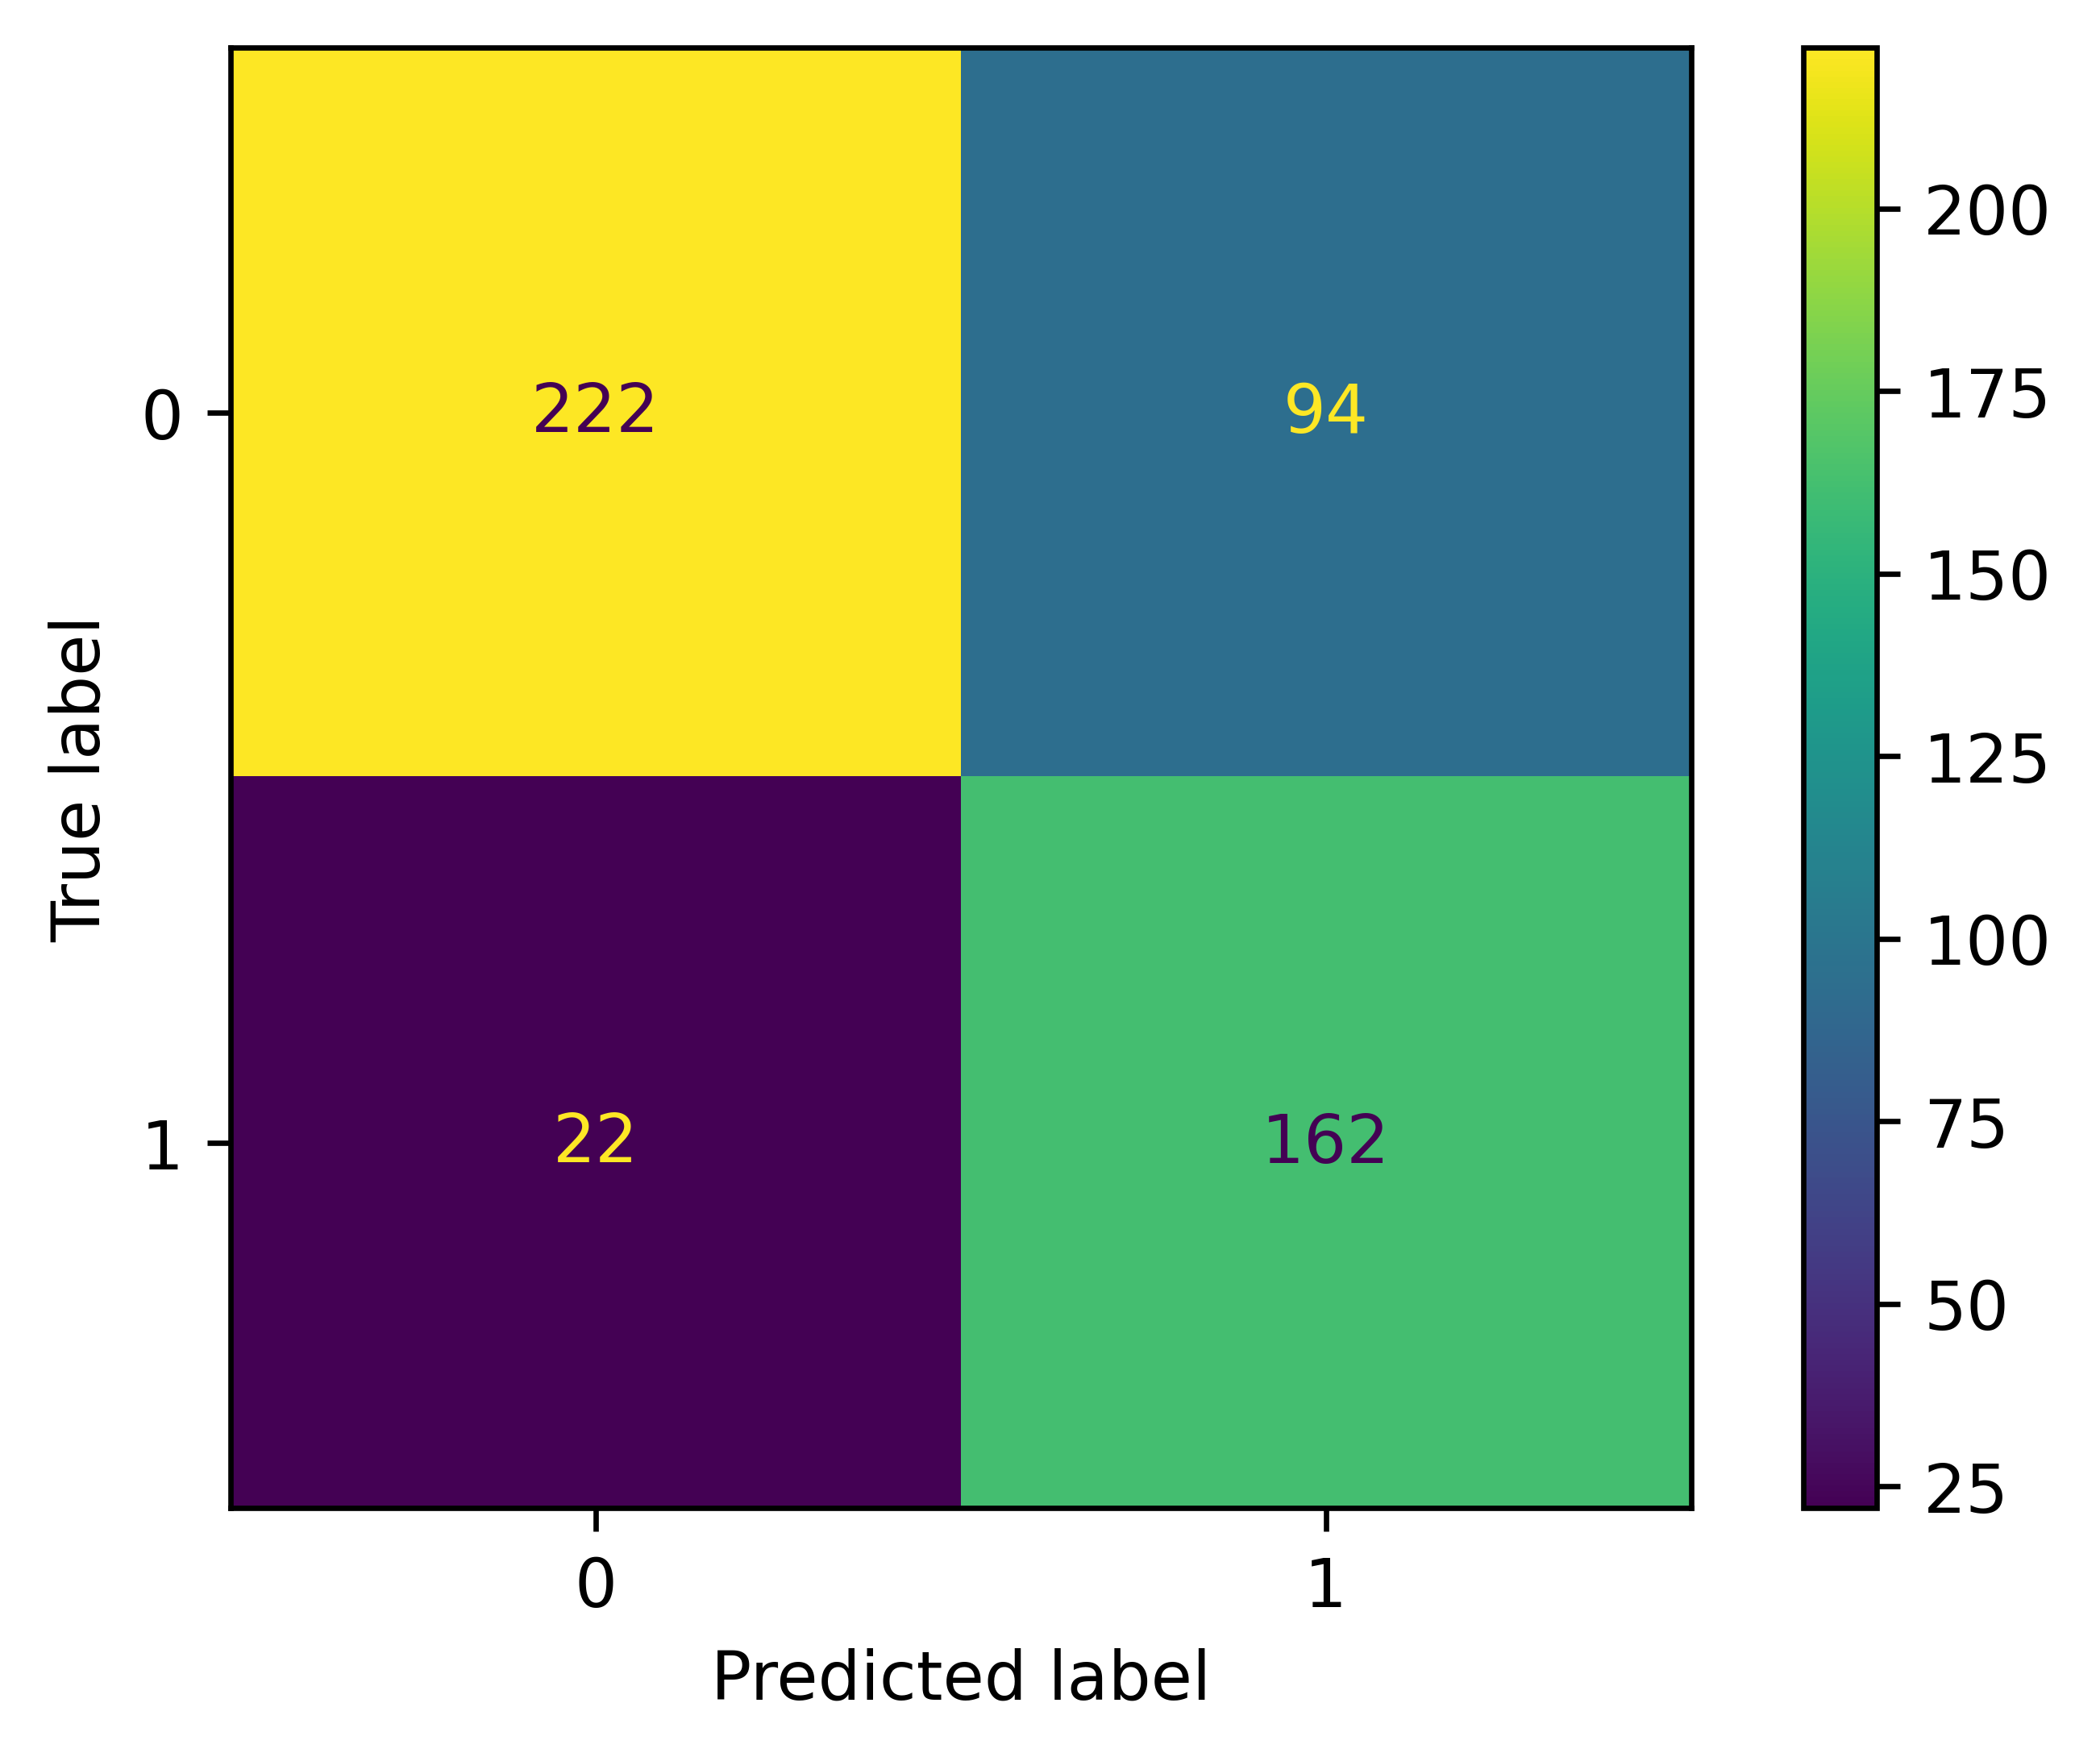
\includegraphics[scale=0.5]{Graphics/cm-th-08-all-patterns.png}}
	\subfigure[Patrón con 27 muestras]{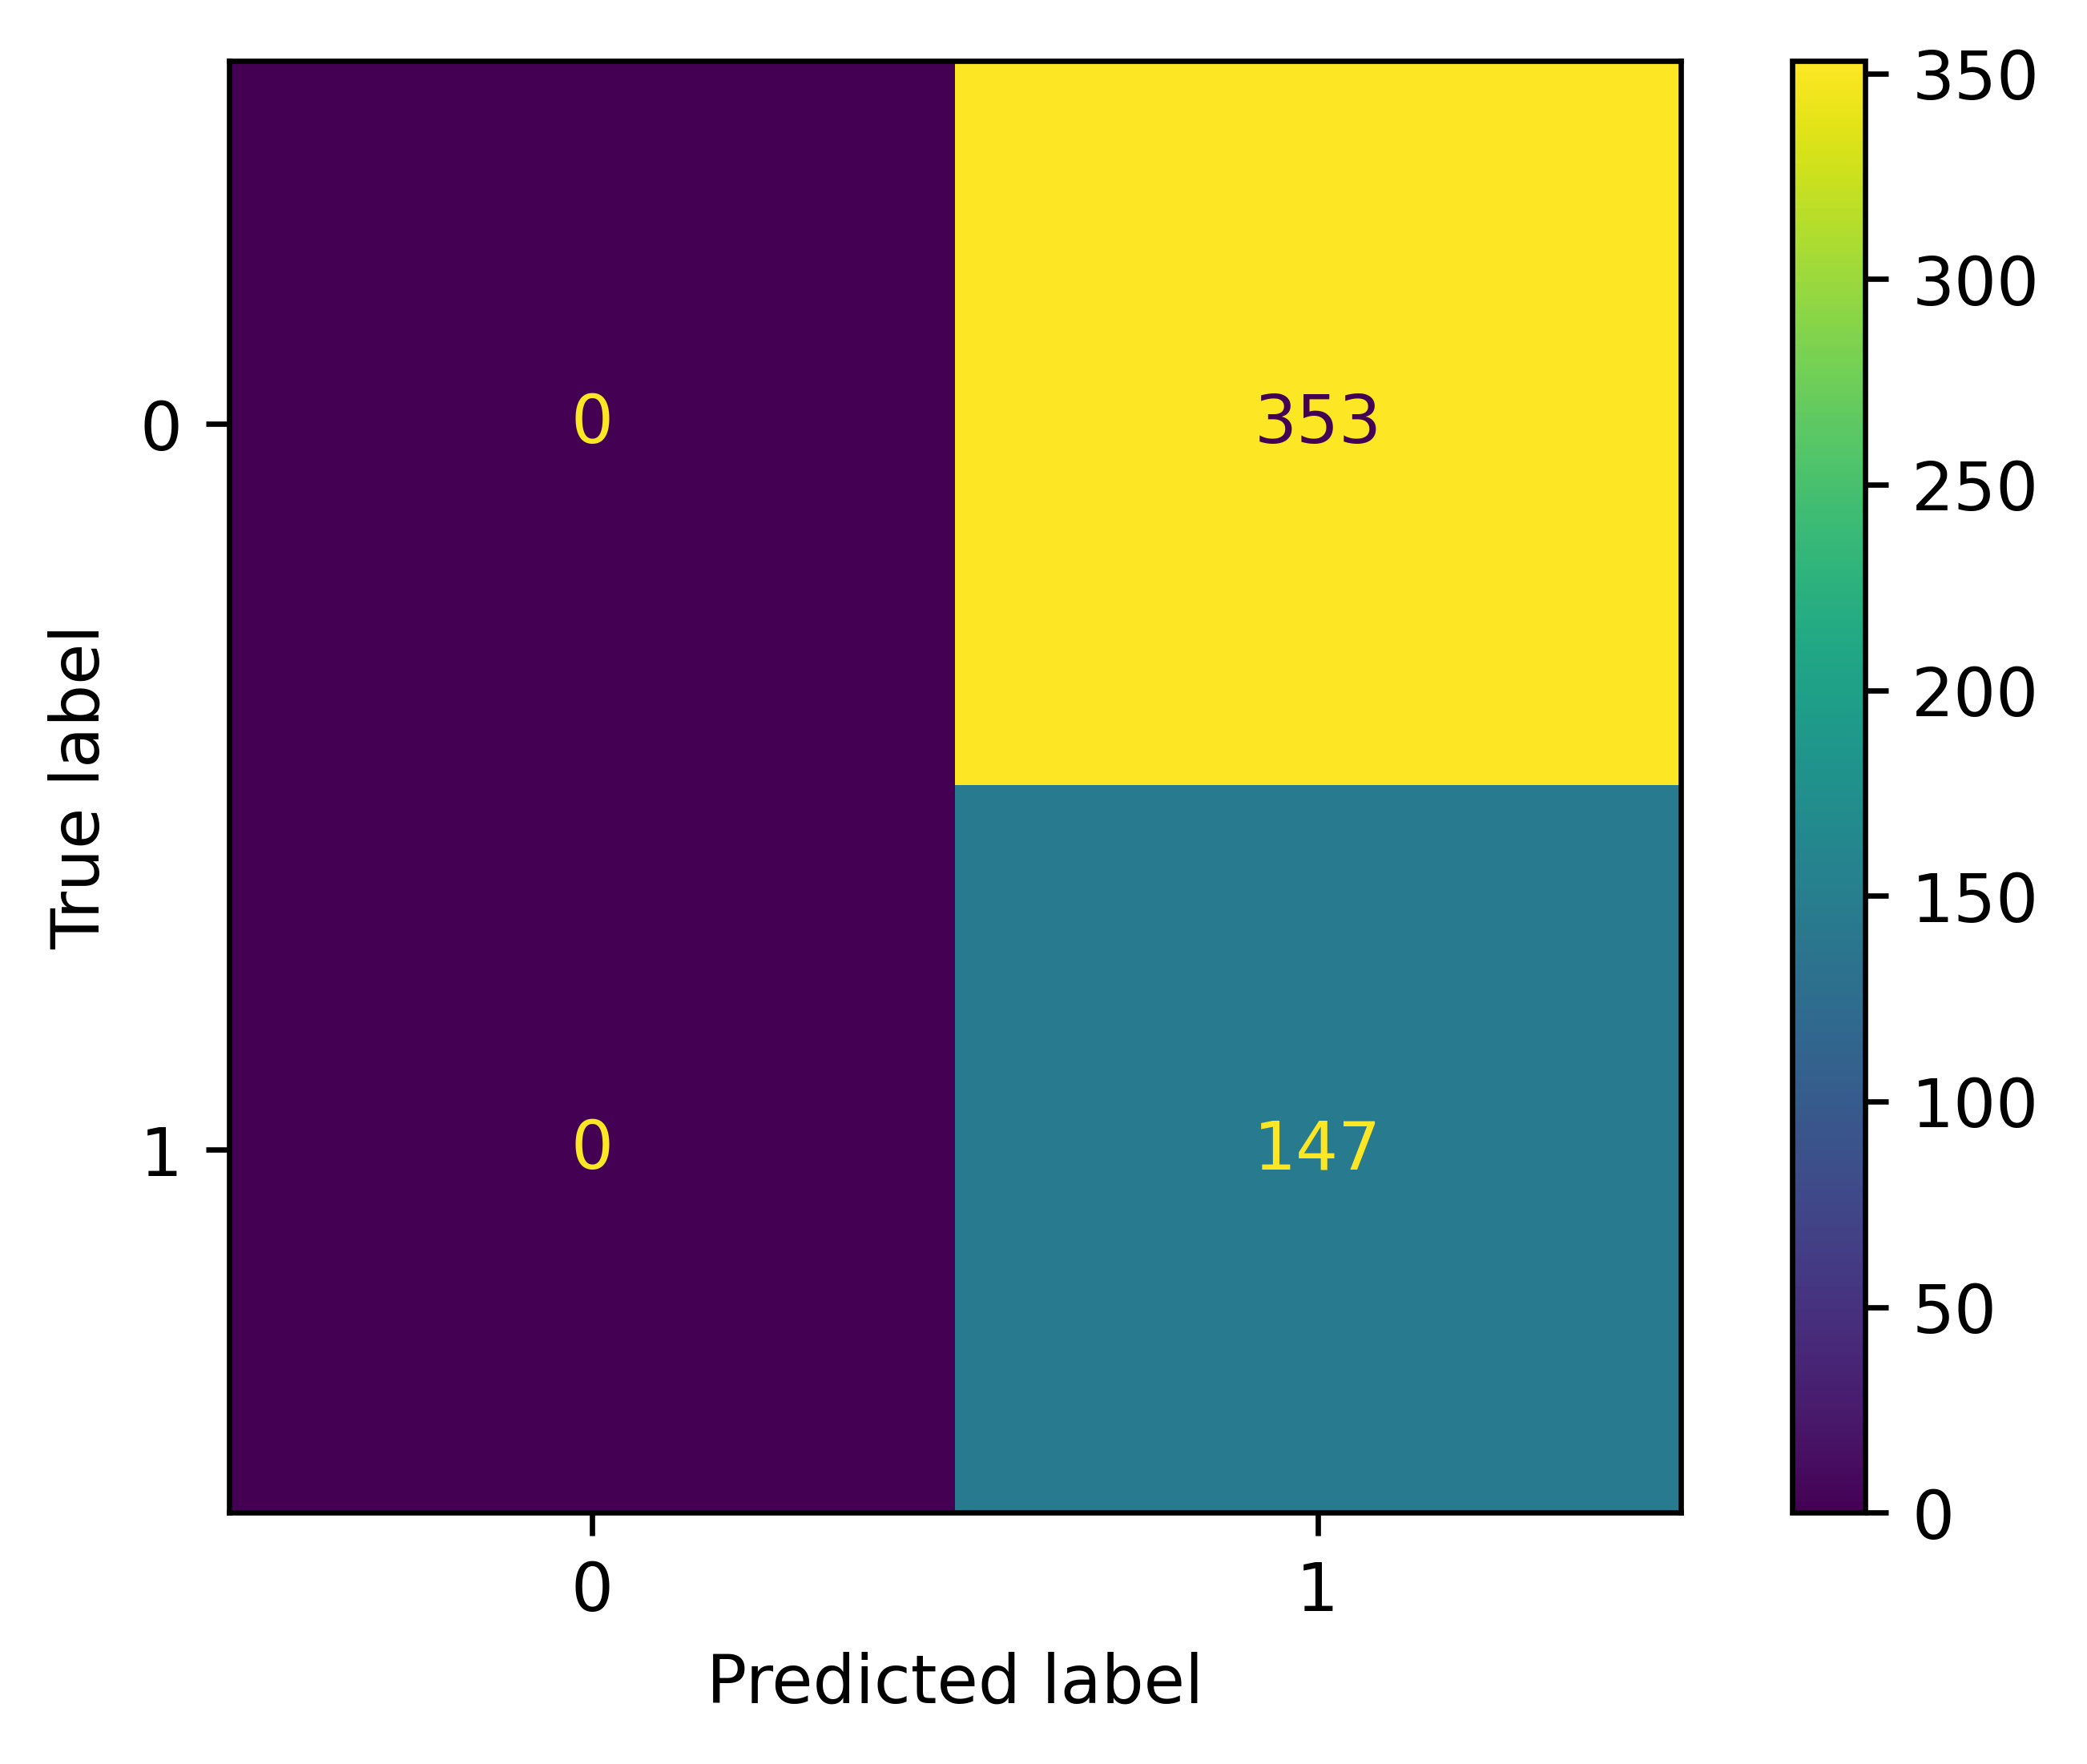
\includegraphics[scale=0.5]{Graphics/cm-th-08-long-pattern.png}}
	\subfigure[Patrón con 19 muestras]{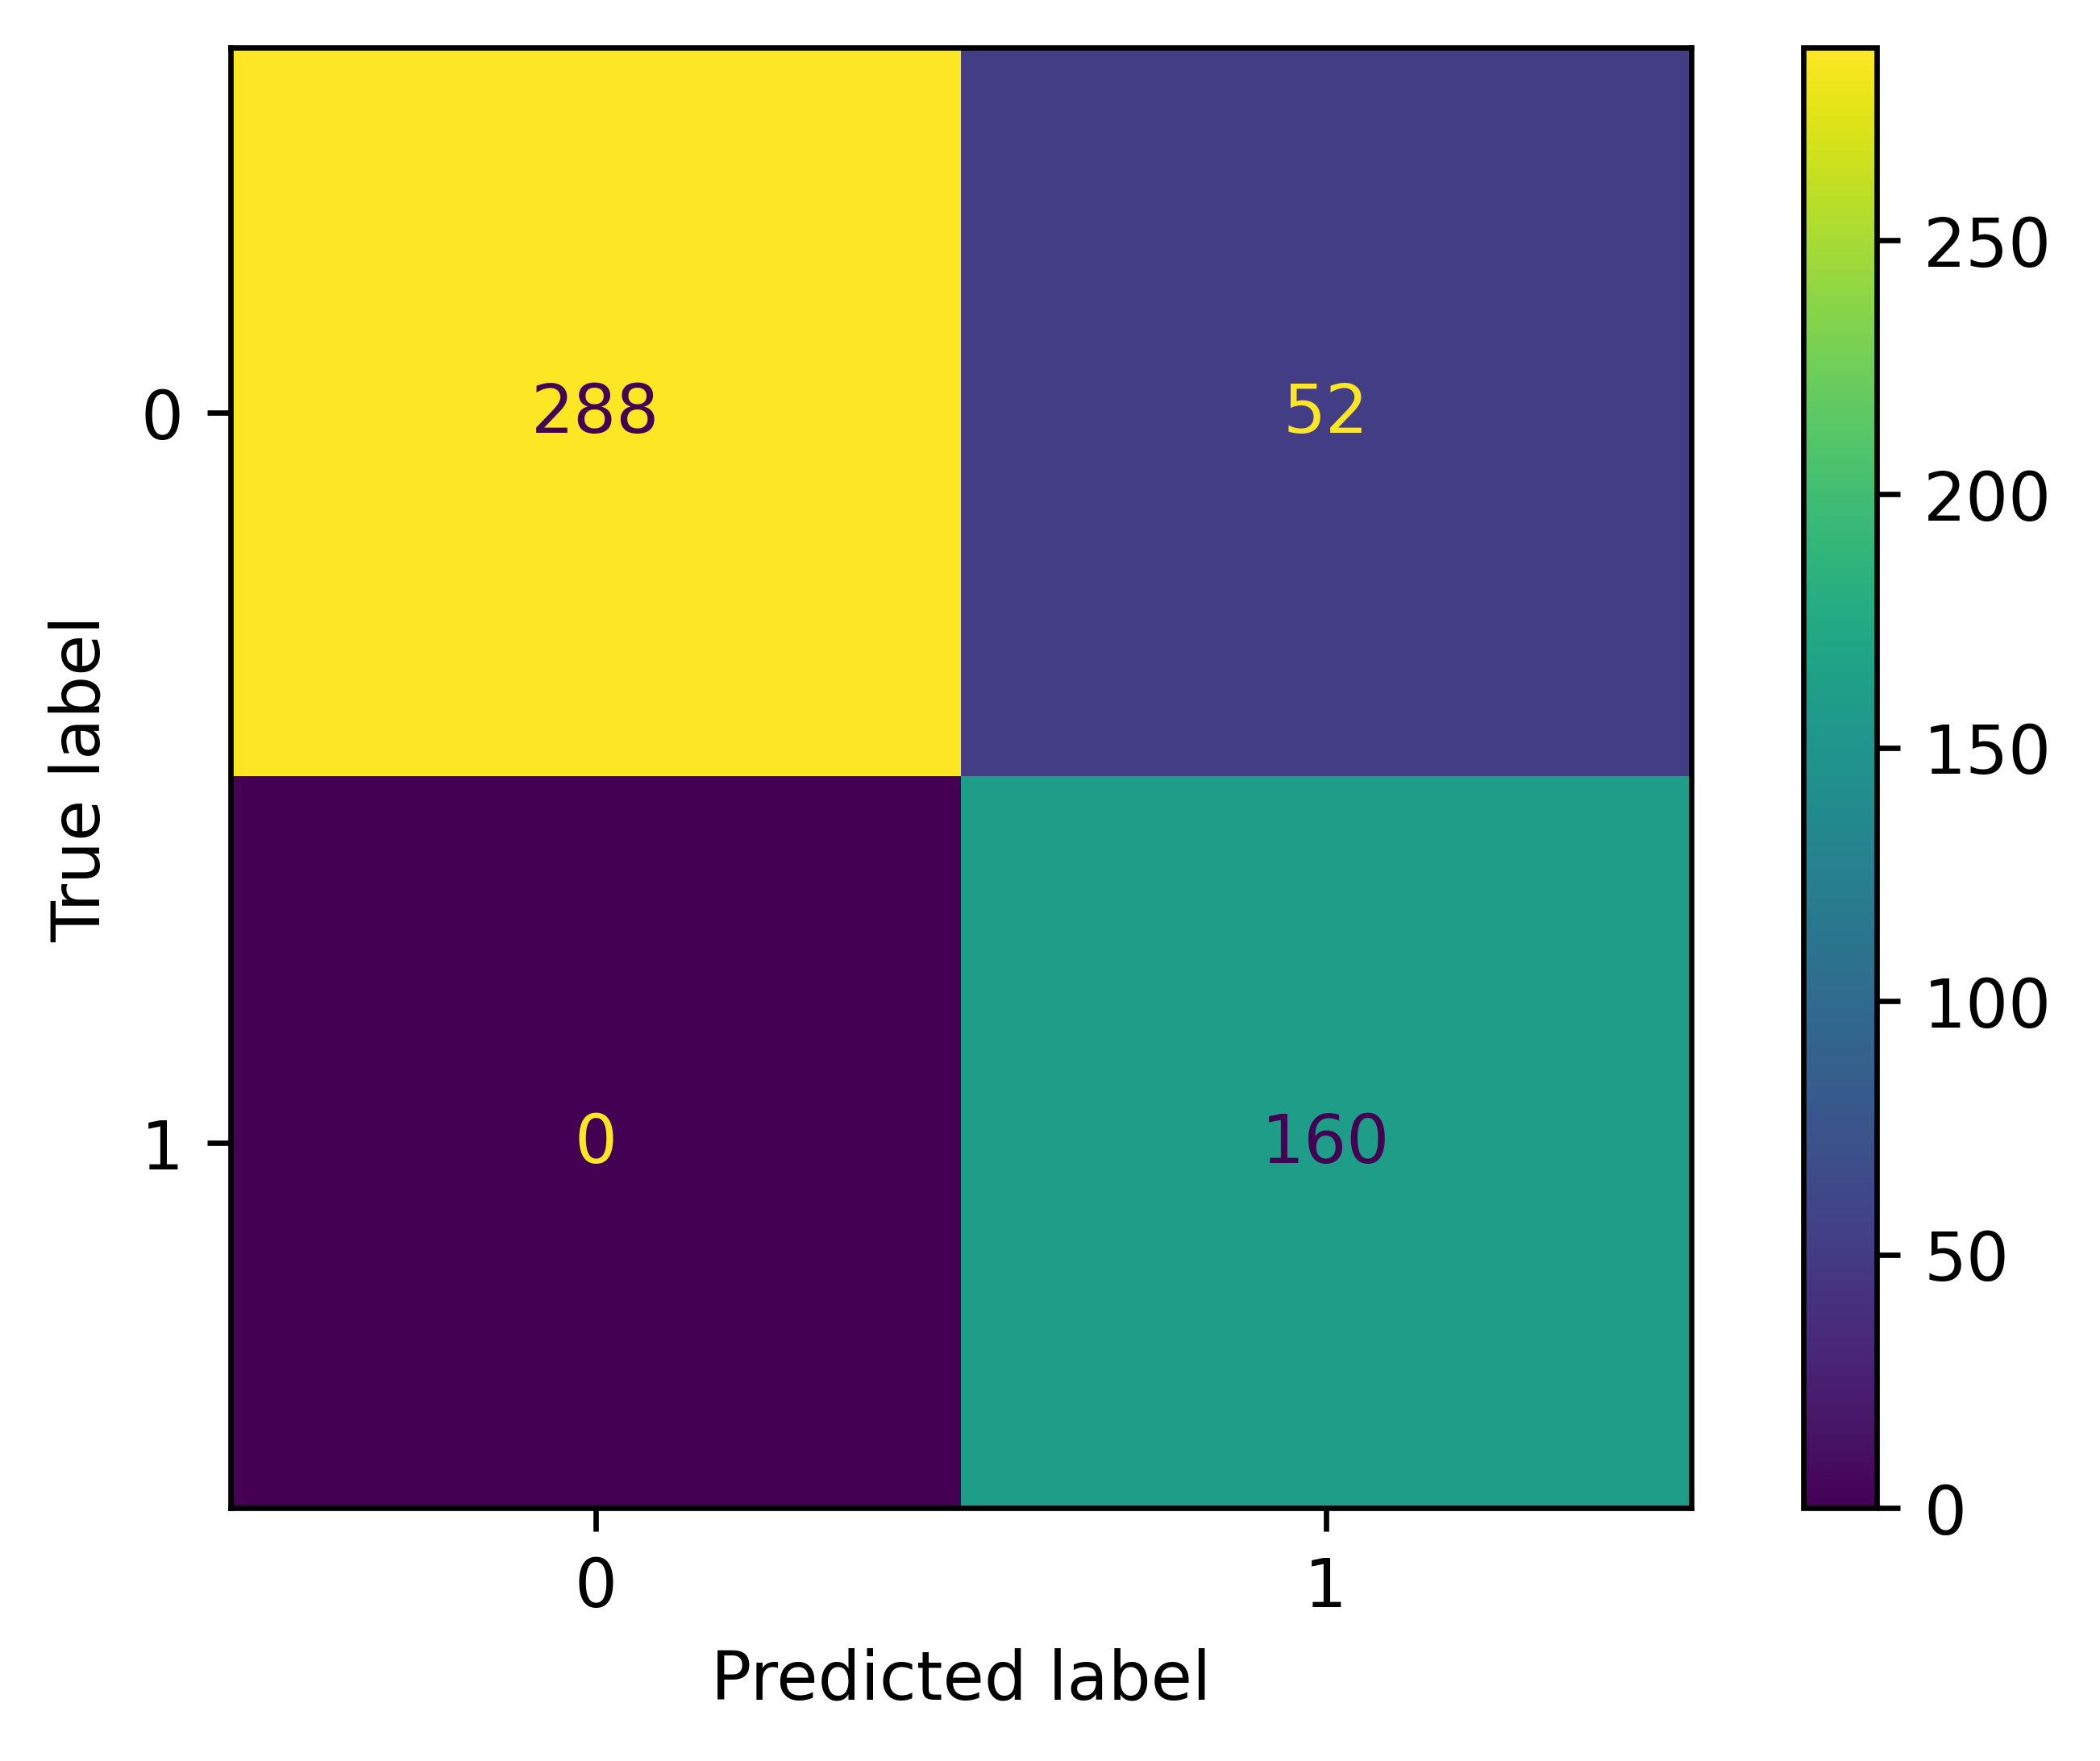
\includegraphics[scale=0.5]{Graphics/cm-th-08-medium-pattern.png}}
	\caption{ Matrices de confusión de cada uno de los experimentos. En todos los casos se usó $th=0.8$.} \label{fig:cm-comparison}
\end{figure} 

\begin{figure}
	\centering
	\subfigure[Varios patrones de entre 15 y 27 muestras]{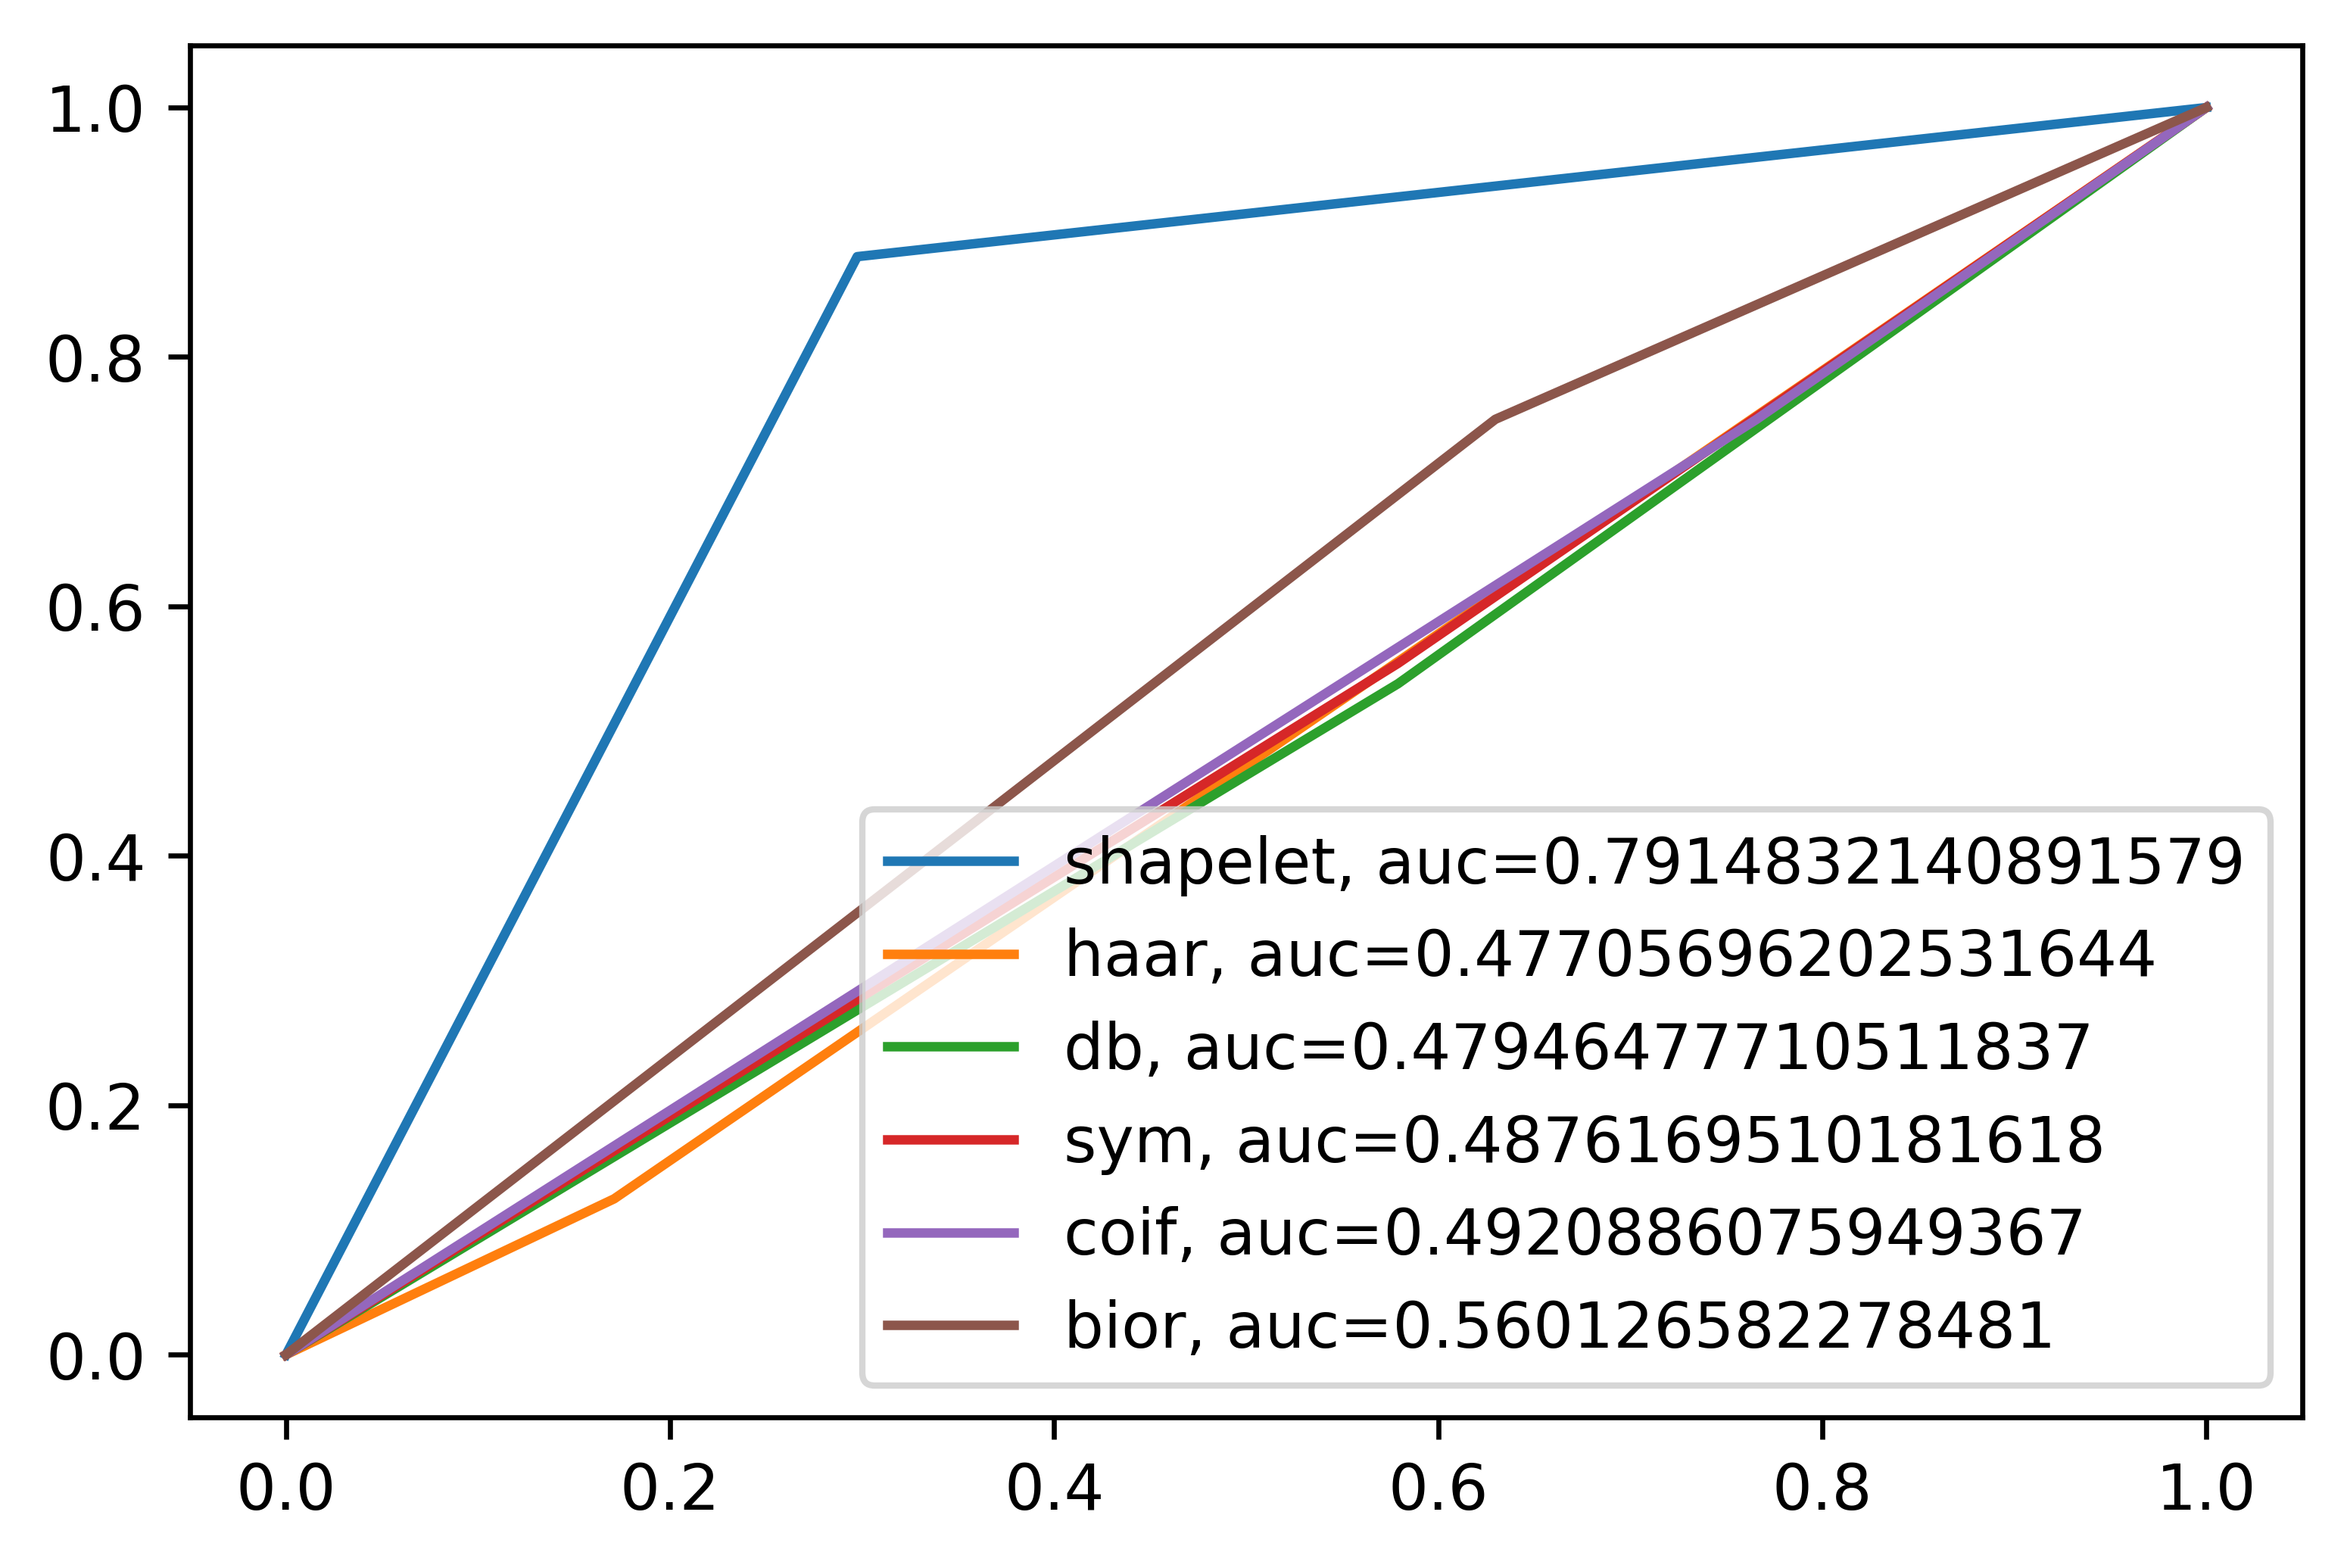
\includegraphics[scale=0.5]{Graphics/roc-th-08-all-patterns.png}}
	\subfigure[Patrón con 27 muestras]{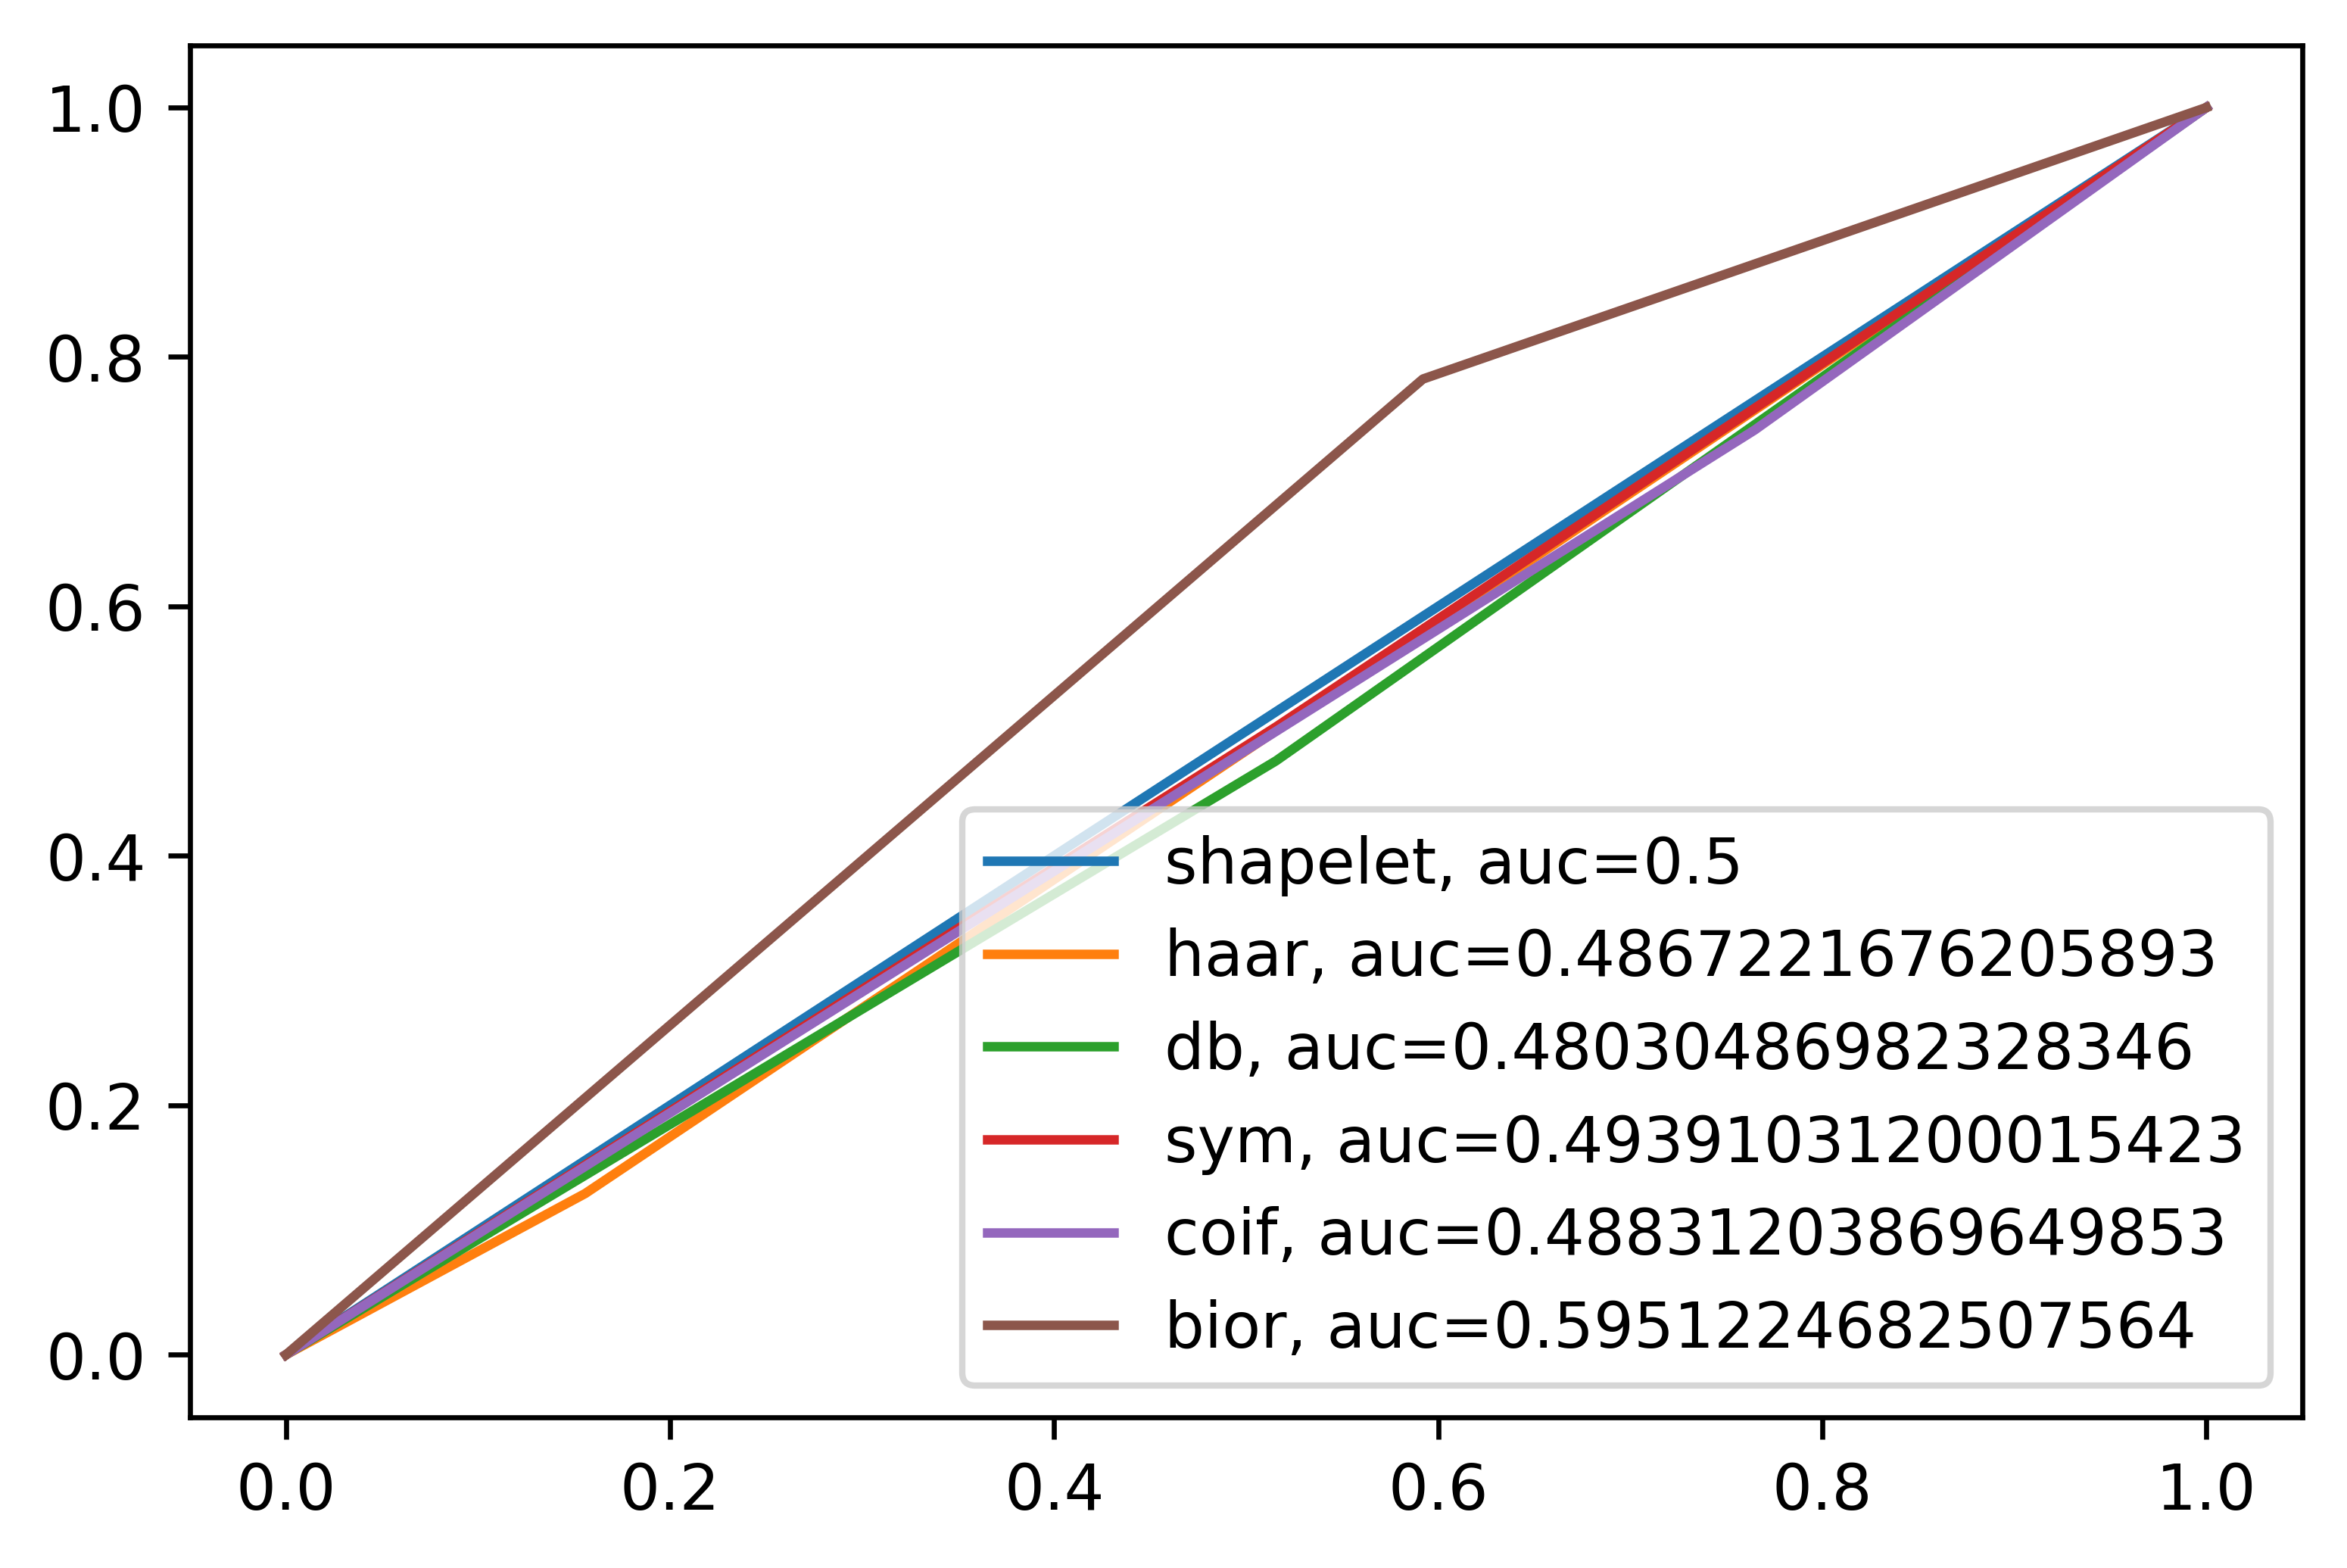
\includegraphics[scale=0.5]{Graphics/roc-th-08-long-pattern.png}}
	\subfigure[Patrón con 19 muestras]{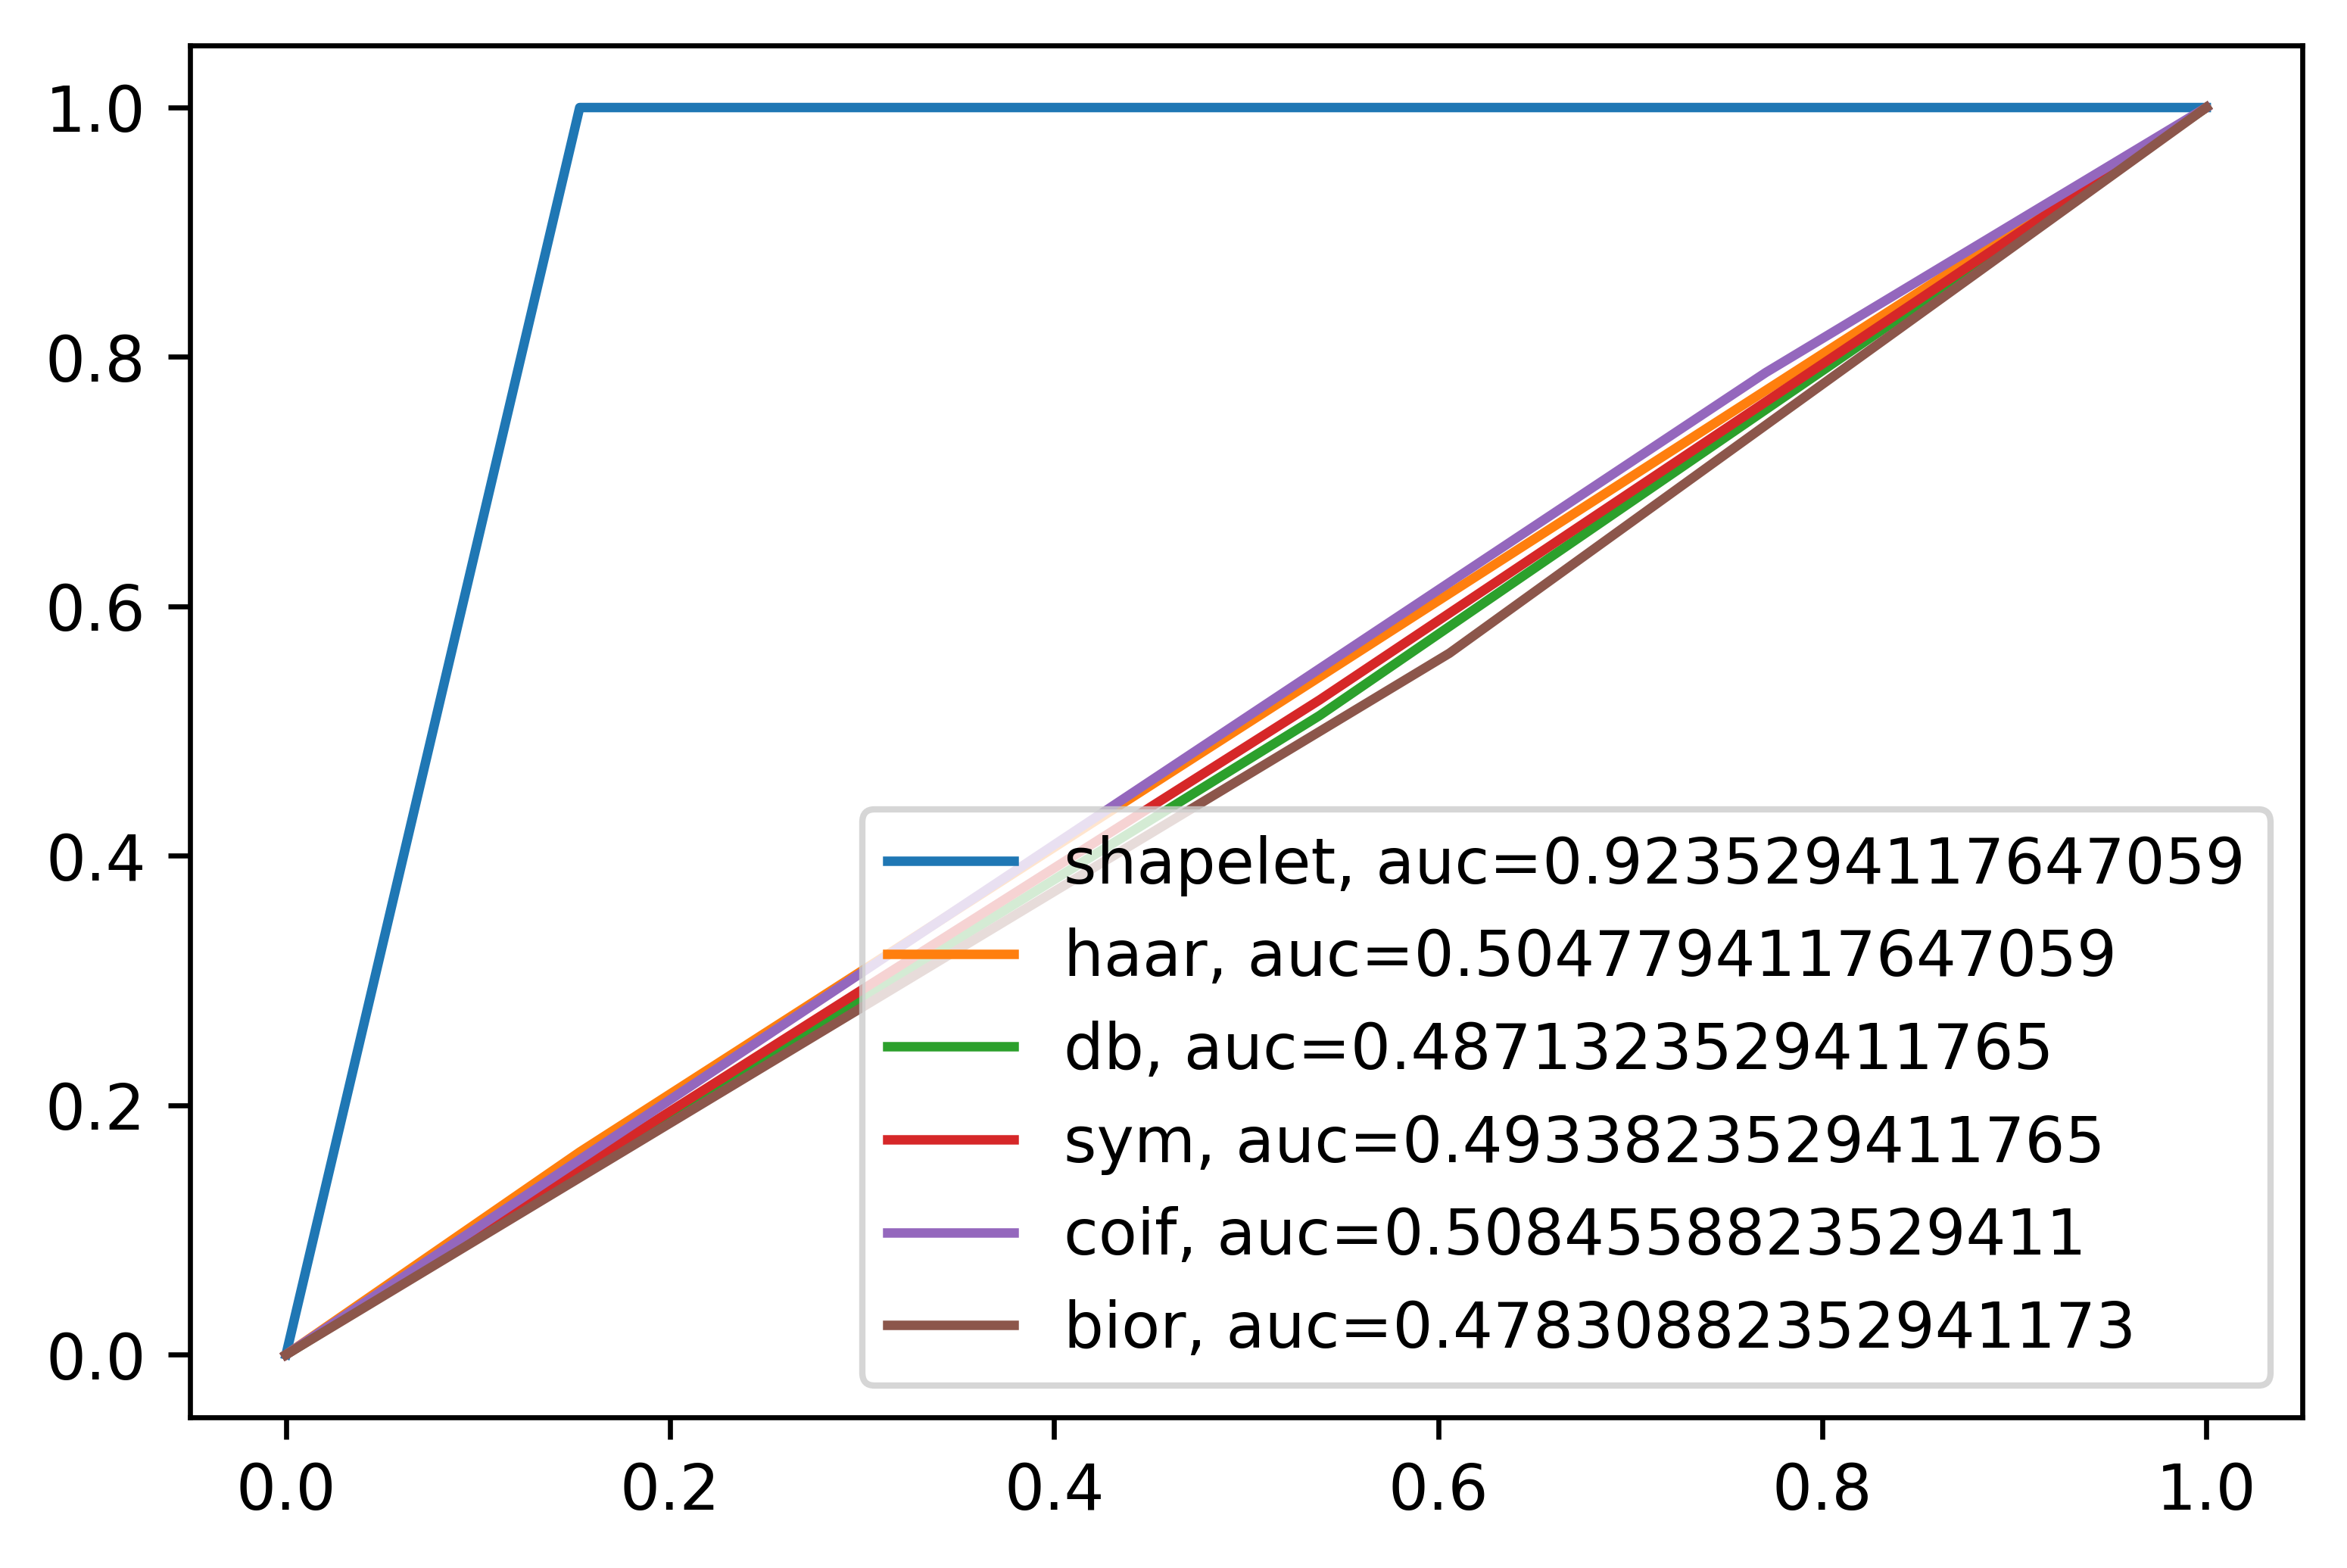
\includegraphics[scale=0.5]{Graphics/roc-th-08-medium-pattern.png}}
	\caption{ Curvas ROC para cada uno de los experimentos. En todos los casos se usó $th=0.8$.} \label{fig:roc-comparison}
\end{figure} 

\begin{figure}
	\centering
	\subfigure[Varios patrones de entre 15 y 27 muestras]{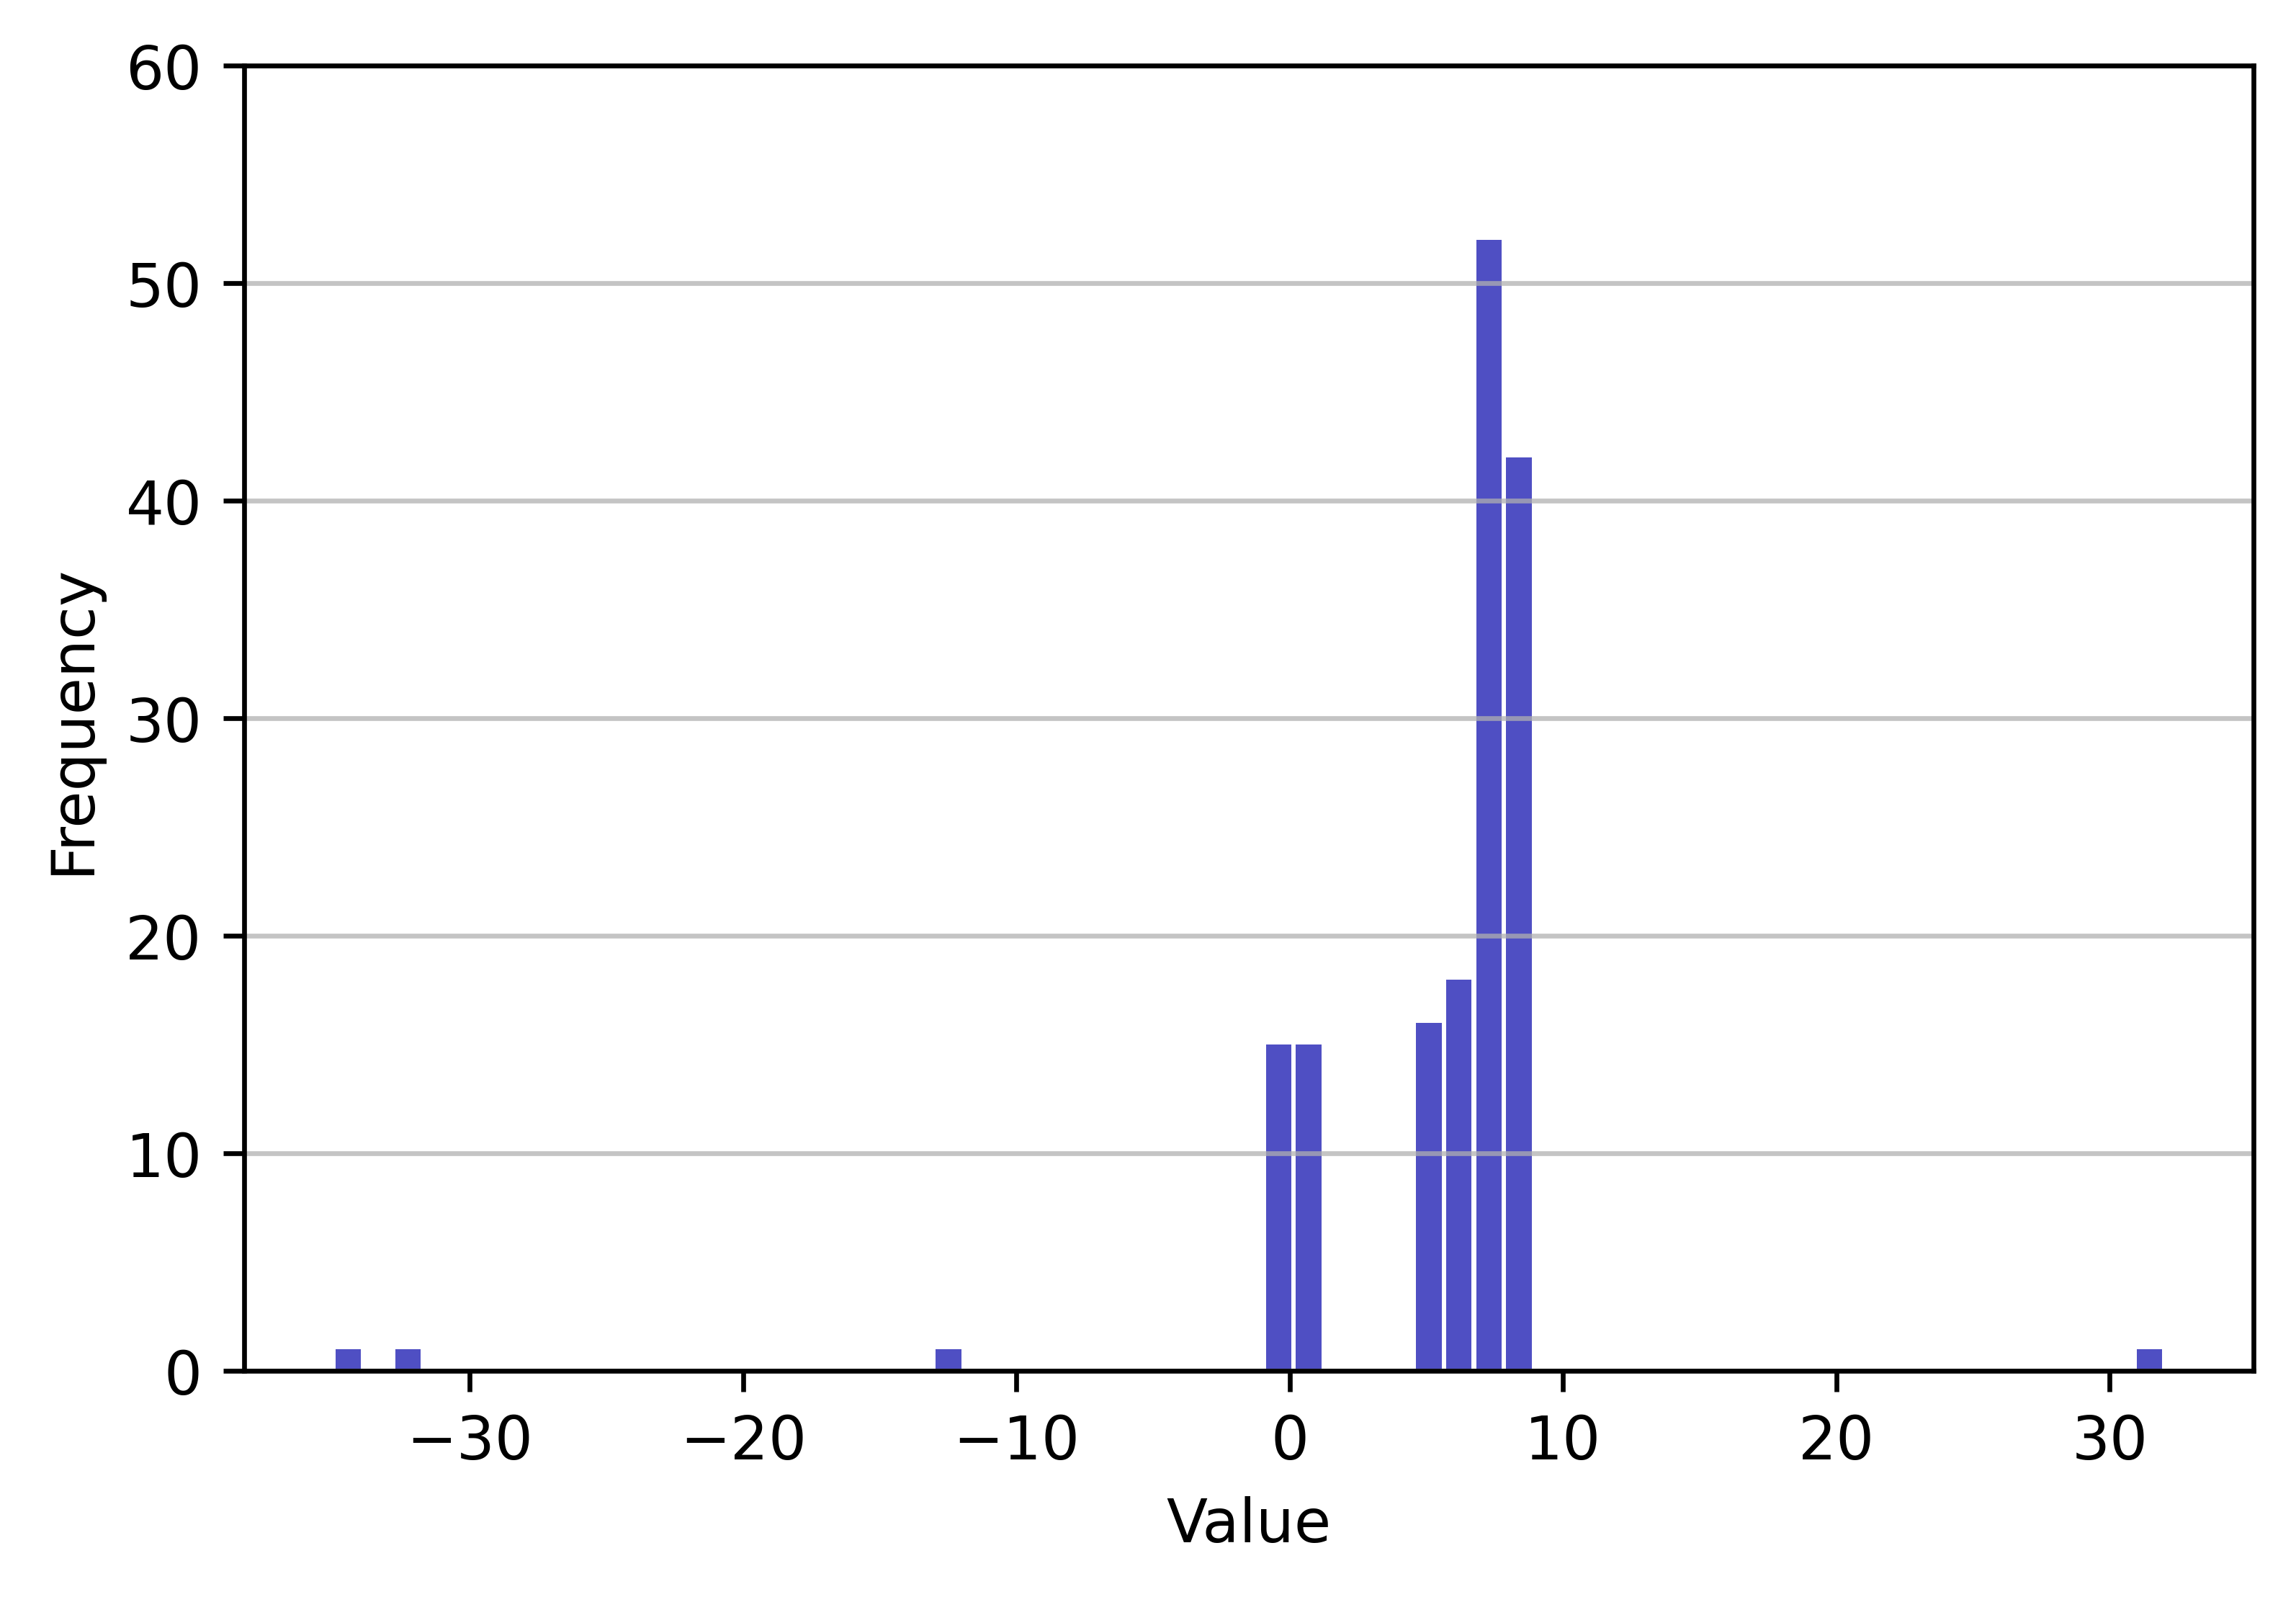
\includegraphics[scale=0.5]{Graphics/histogram-pos-all-patterns.png}}
	\subfigure[Patrón con 19 muestras]{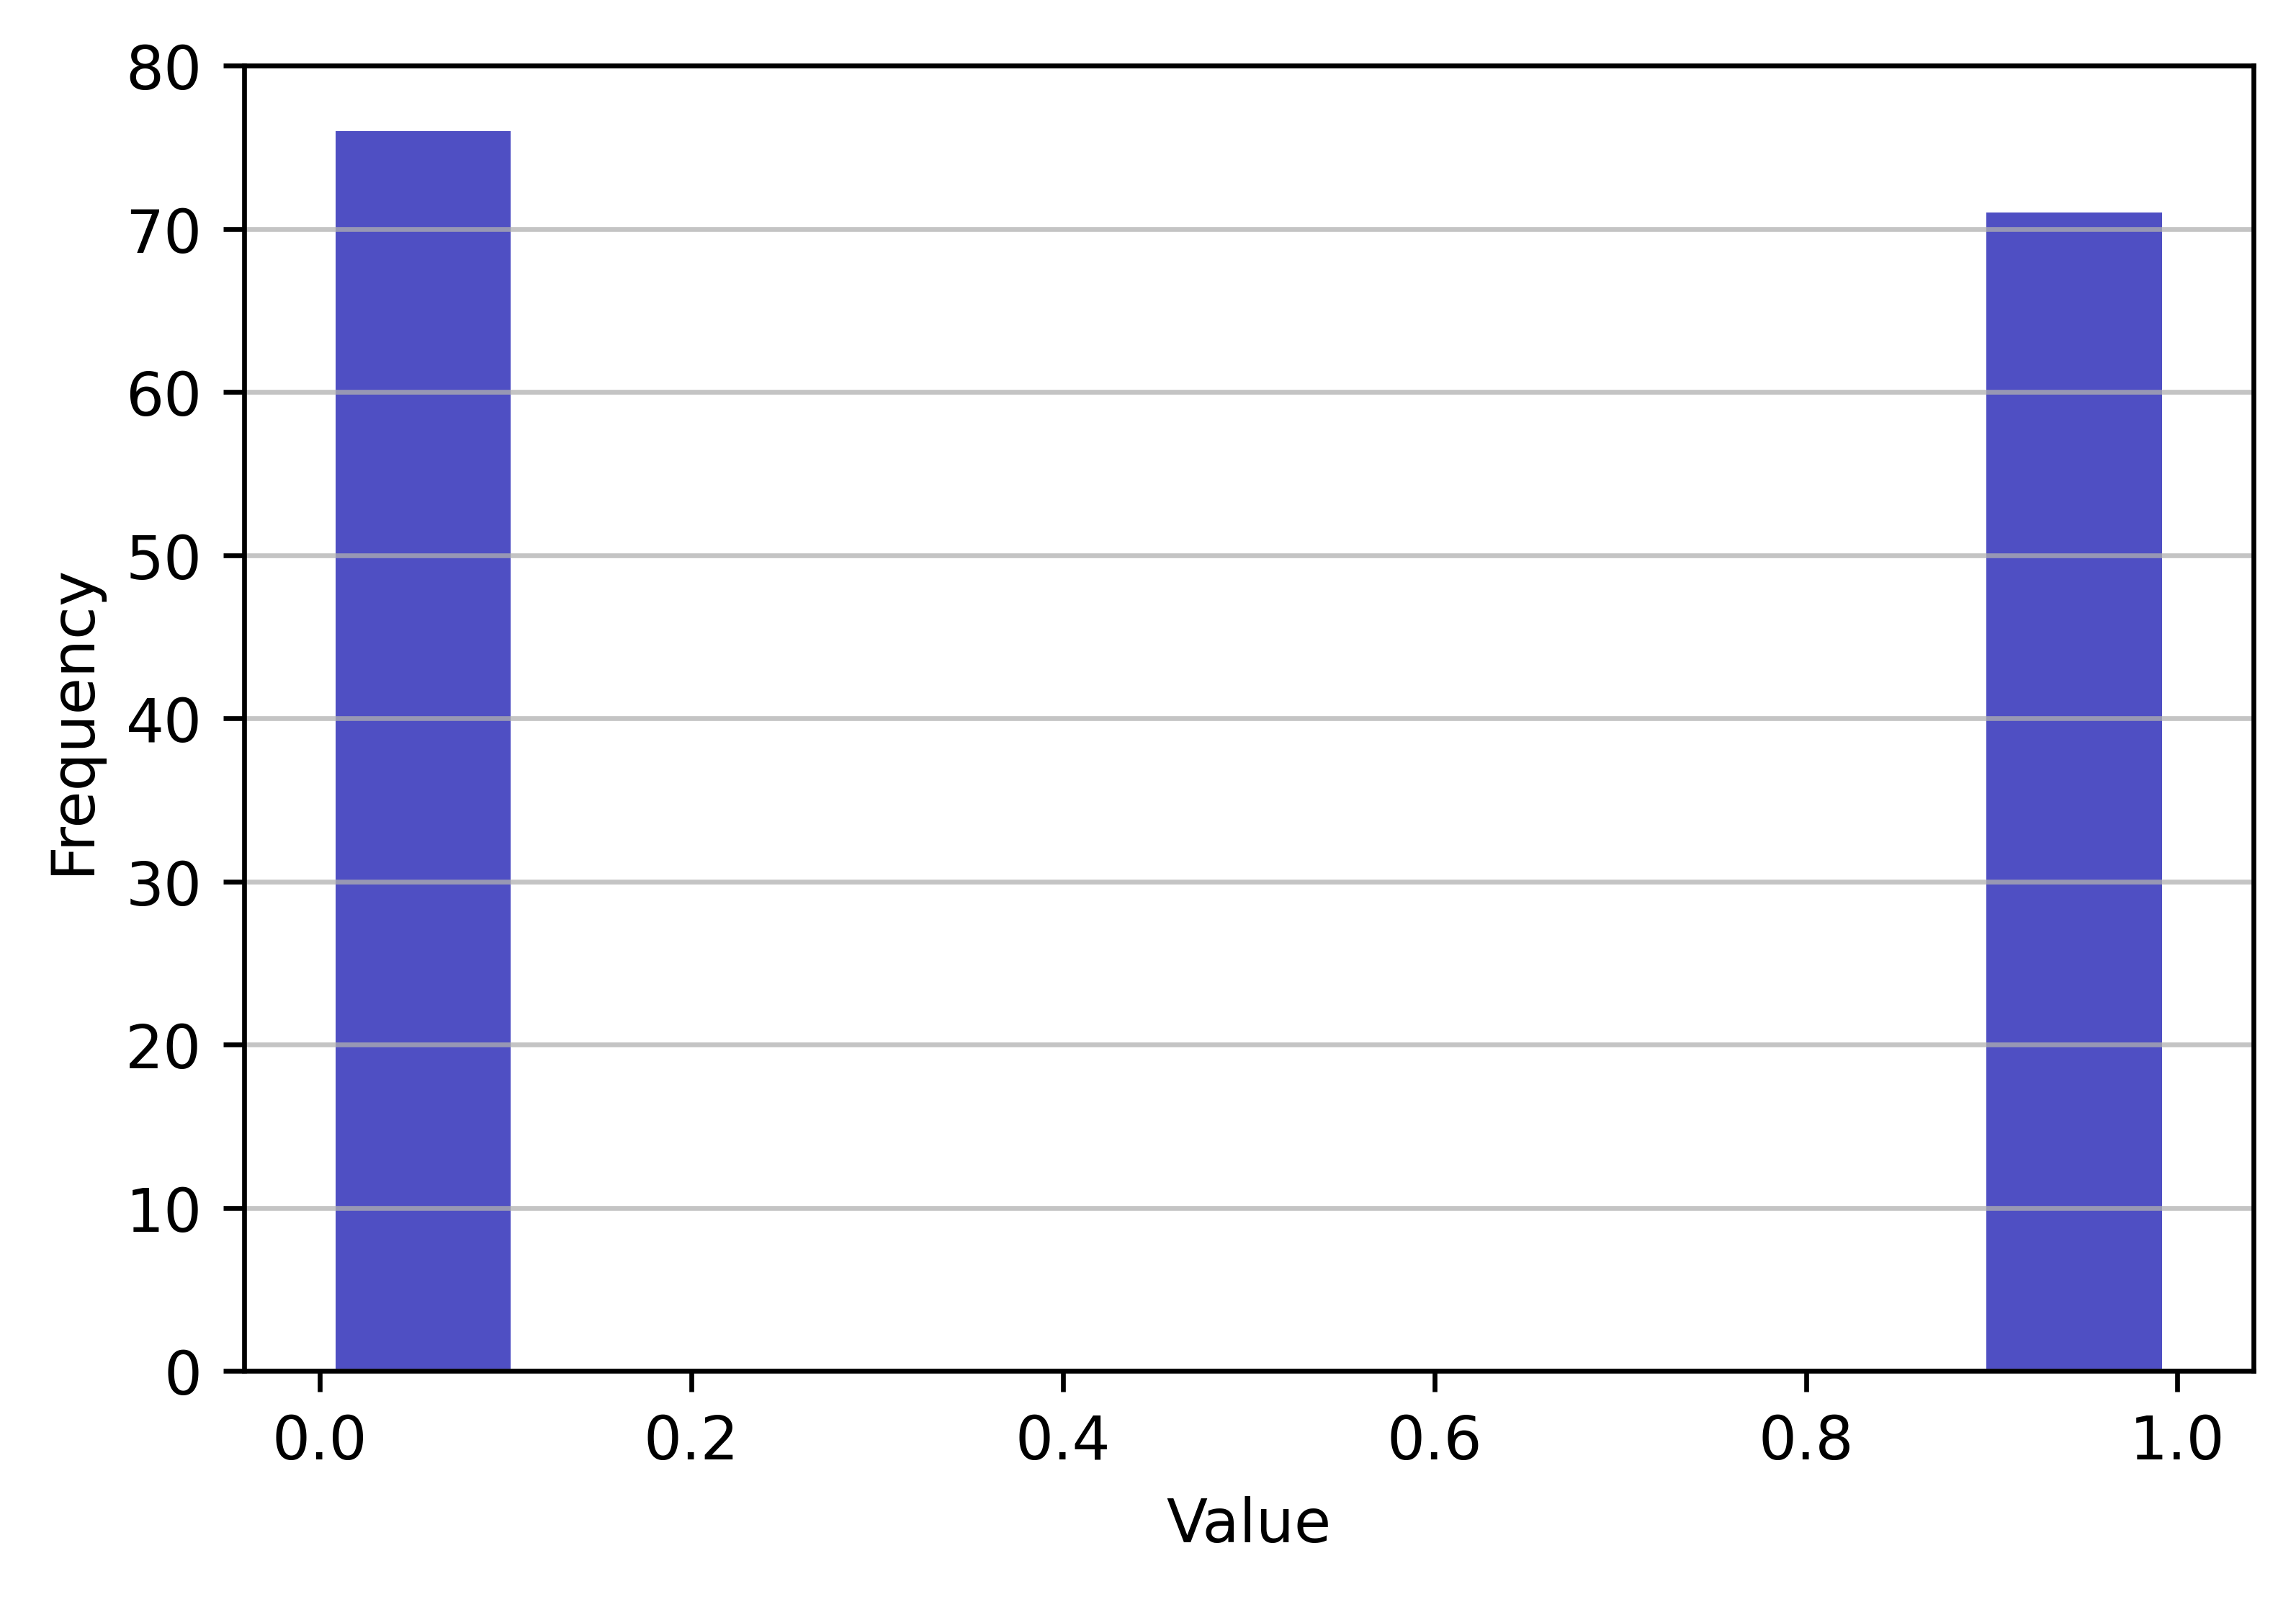
\includegraphics[scale=0.5]{Graphics/histogram-pos-long-pattern.png}}
	\subfigure[Patrón con 27 muestras]{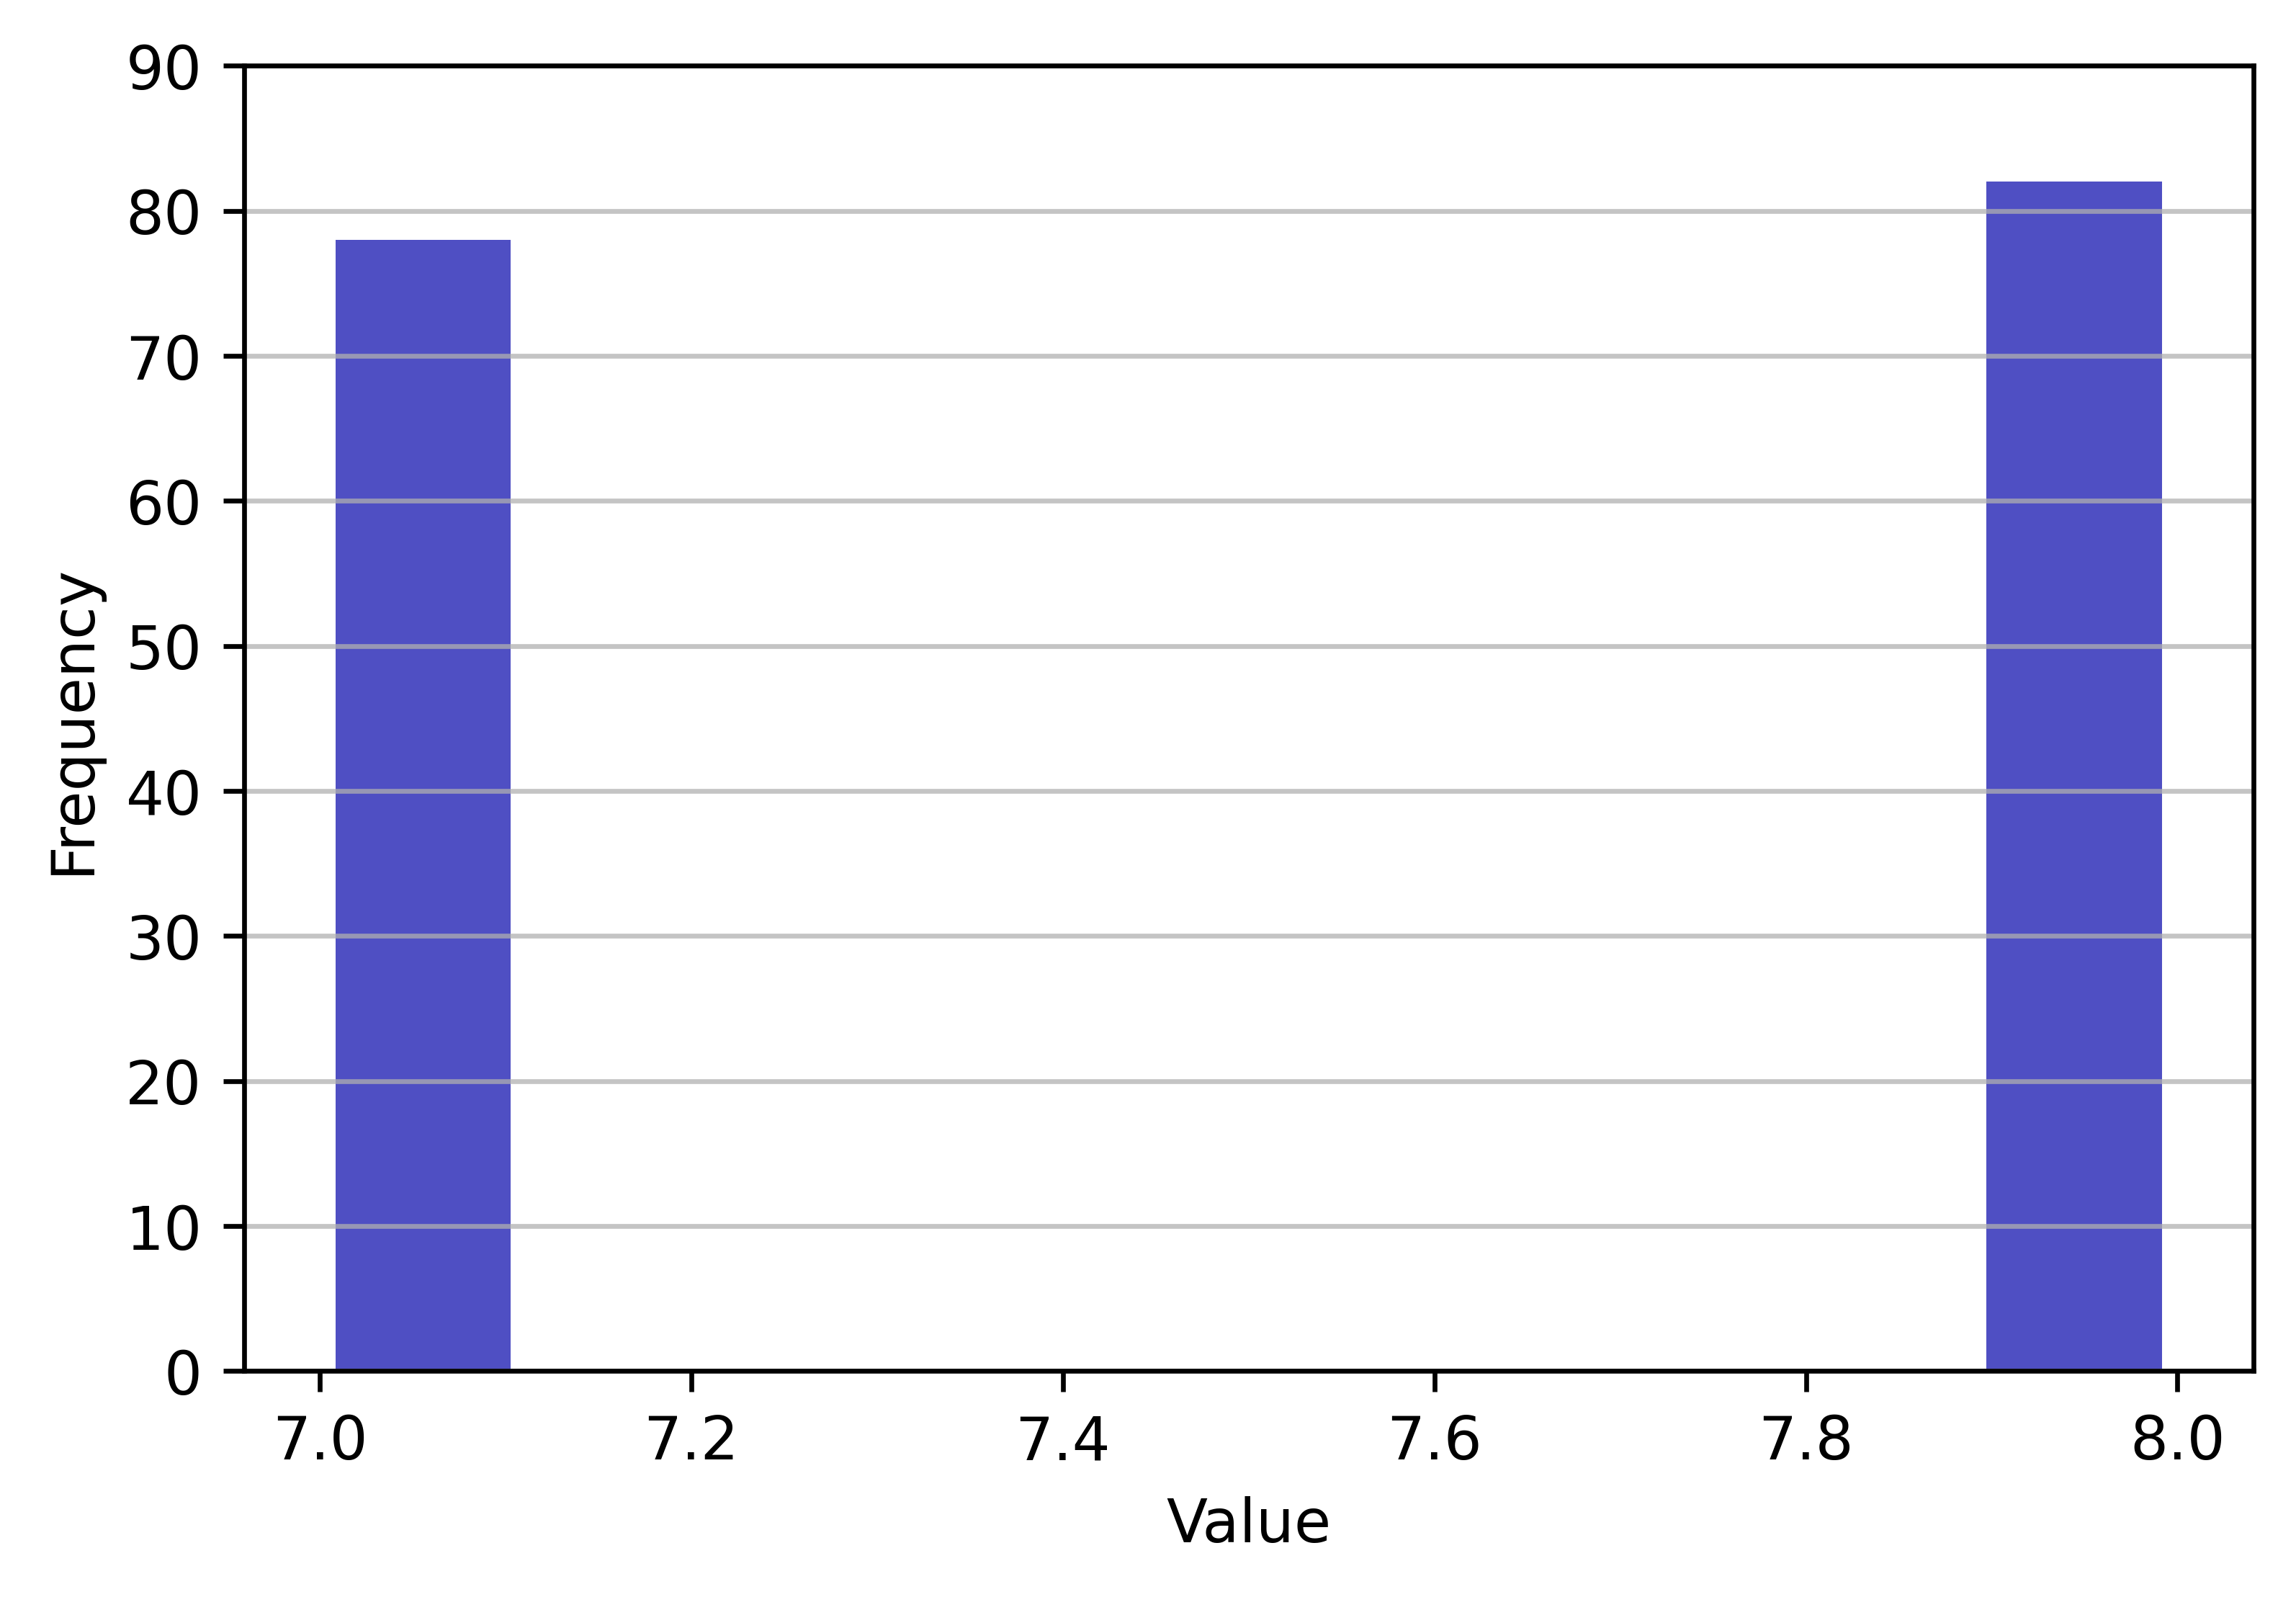
\includegraphics[scale=0.5]{Graphics/histogram-pos-medium-pattern.png}}
	\caption{ Histogramas con las frecuencias de los valores de las diferencias entre la posición real del patrón y la que predice el algoritmo.} \label{fig:hist-comparison}
\end{figure} 

\begin{figure}
	\centering
	\subfigure[Matriz de confusión]{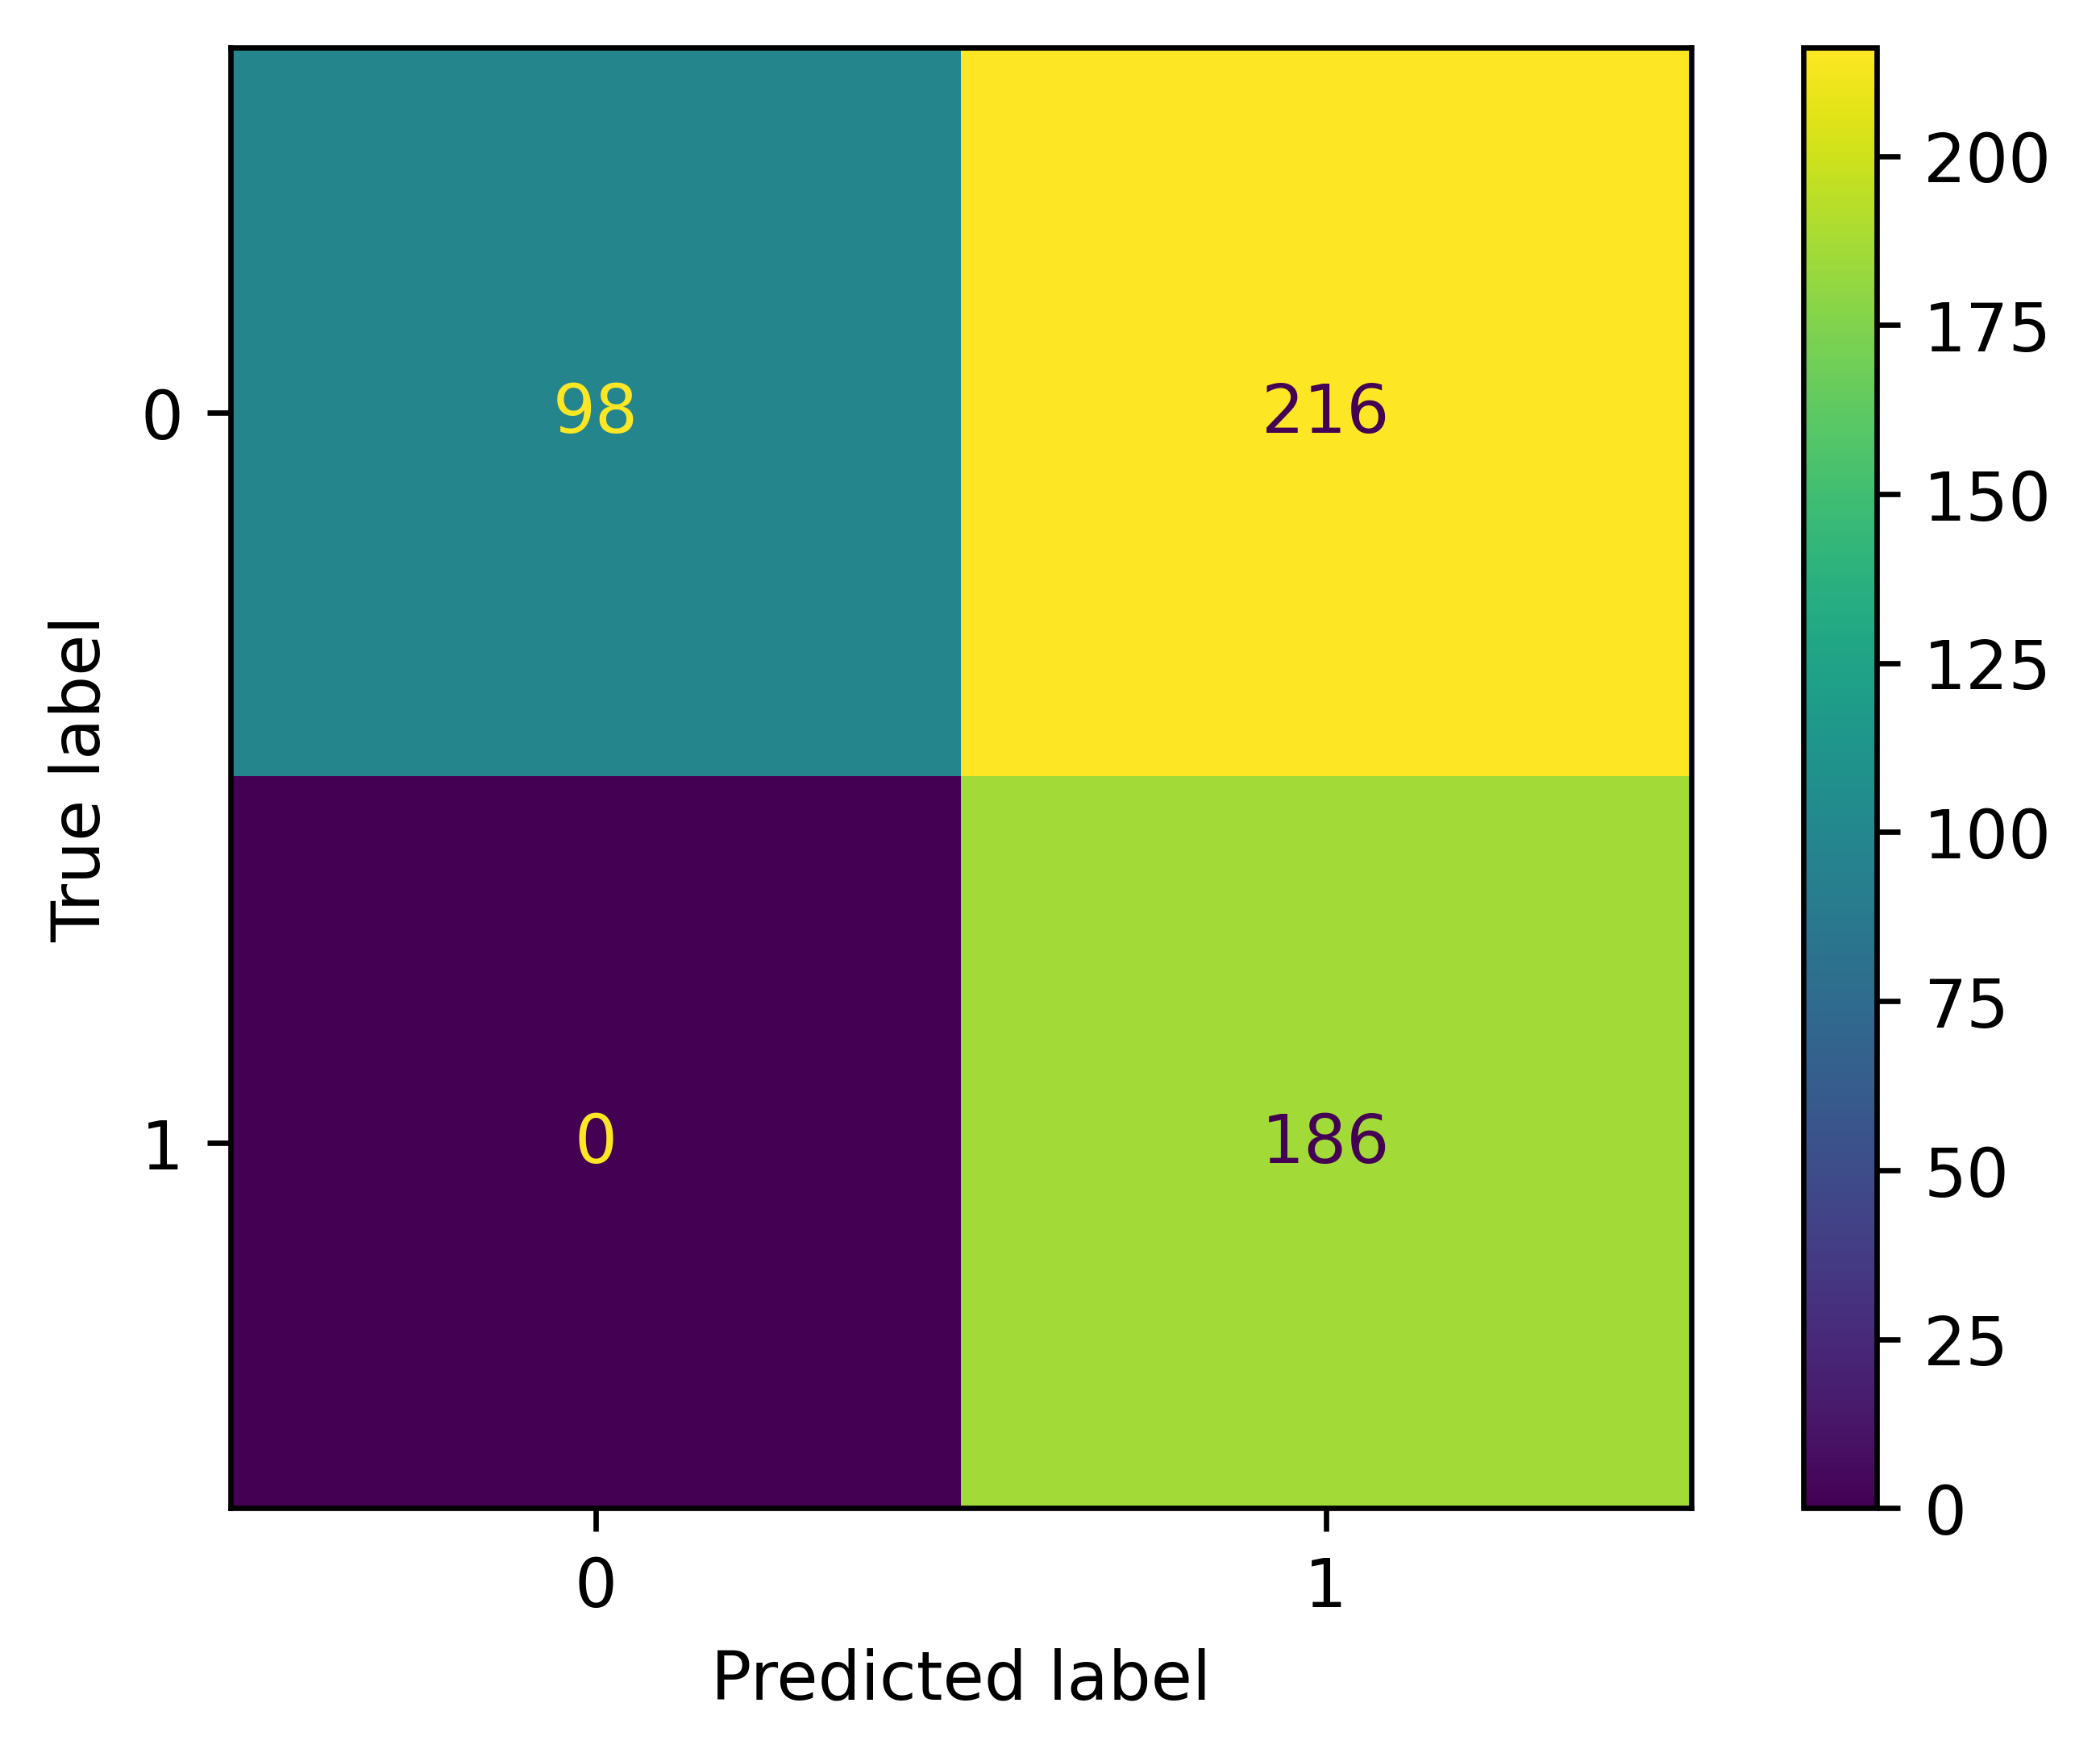
\includegraphics[scale=0.5]{Graphics/cm-th-06.png}}
	\subfigure[Curva ROC]{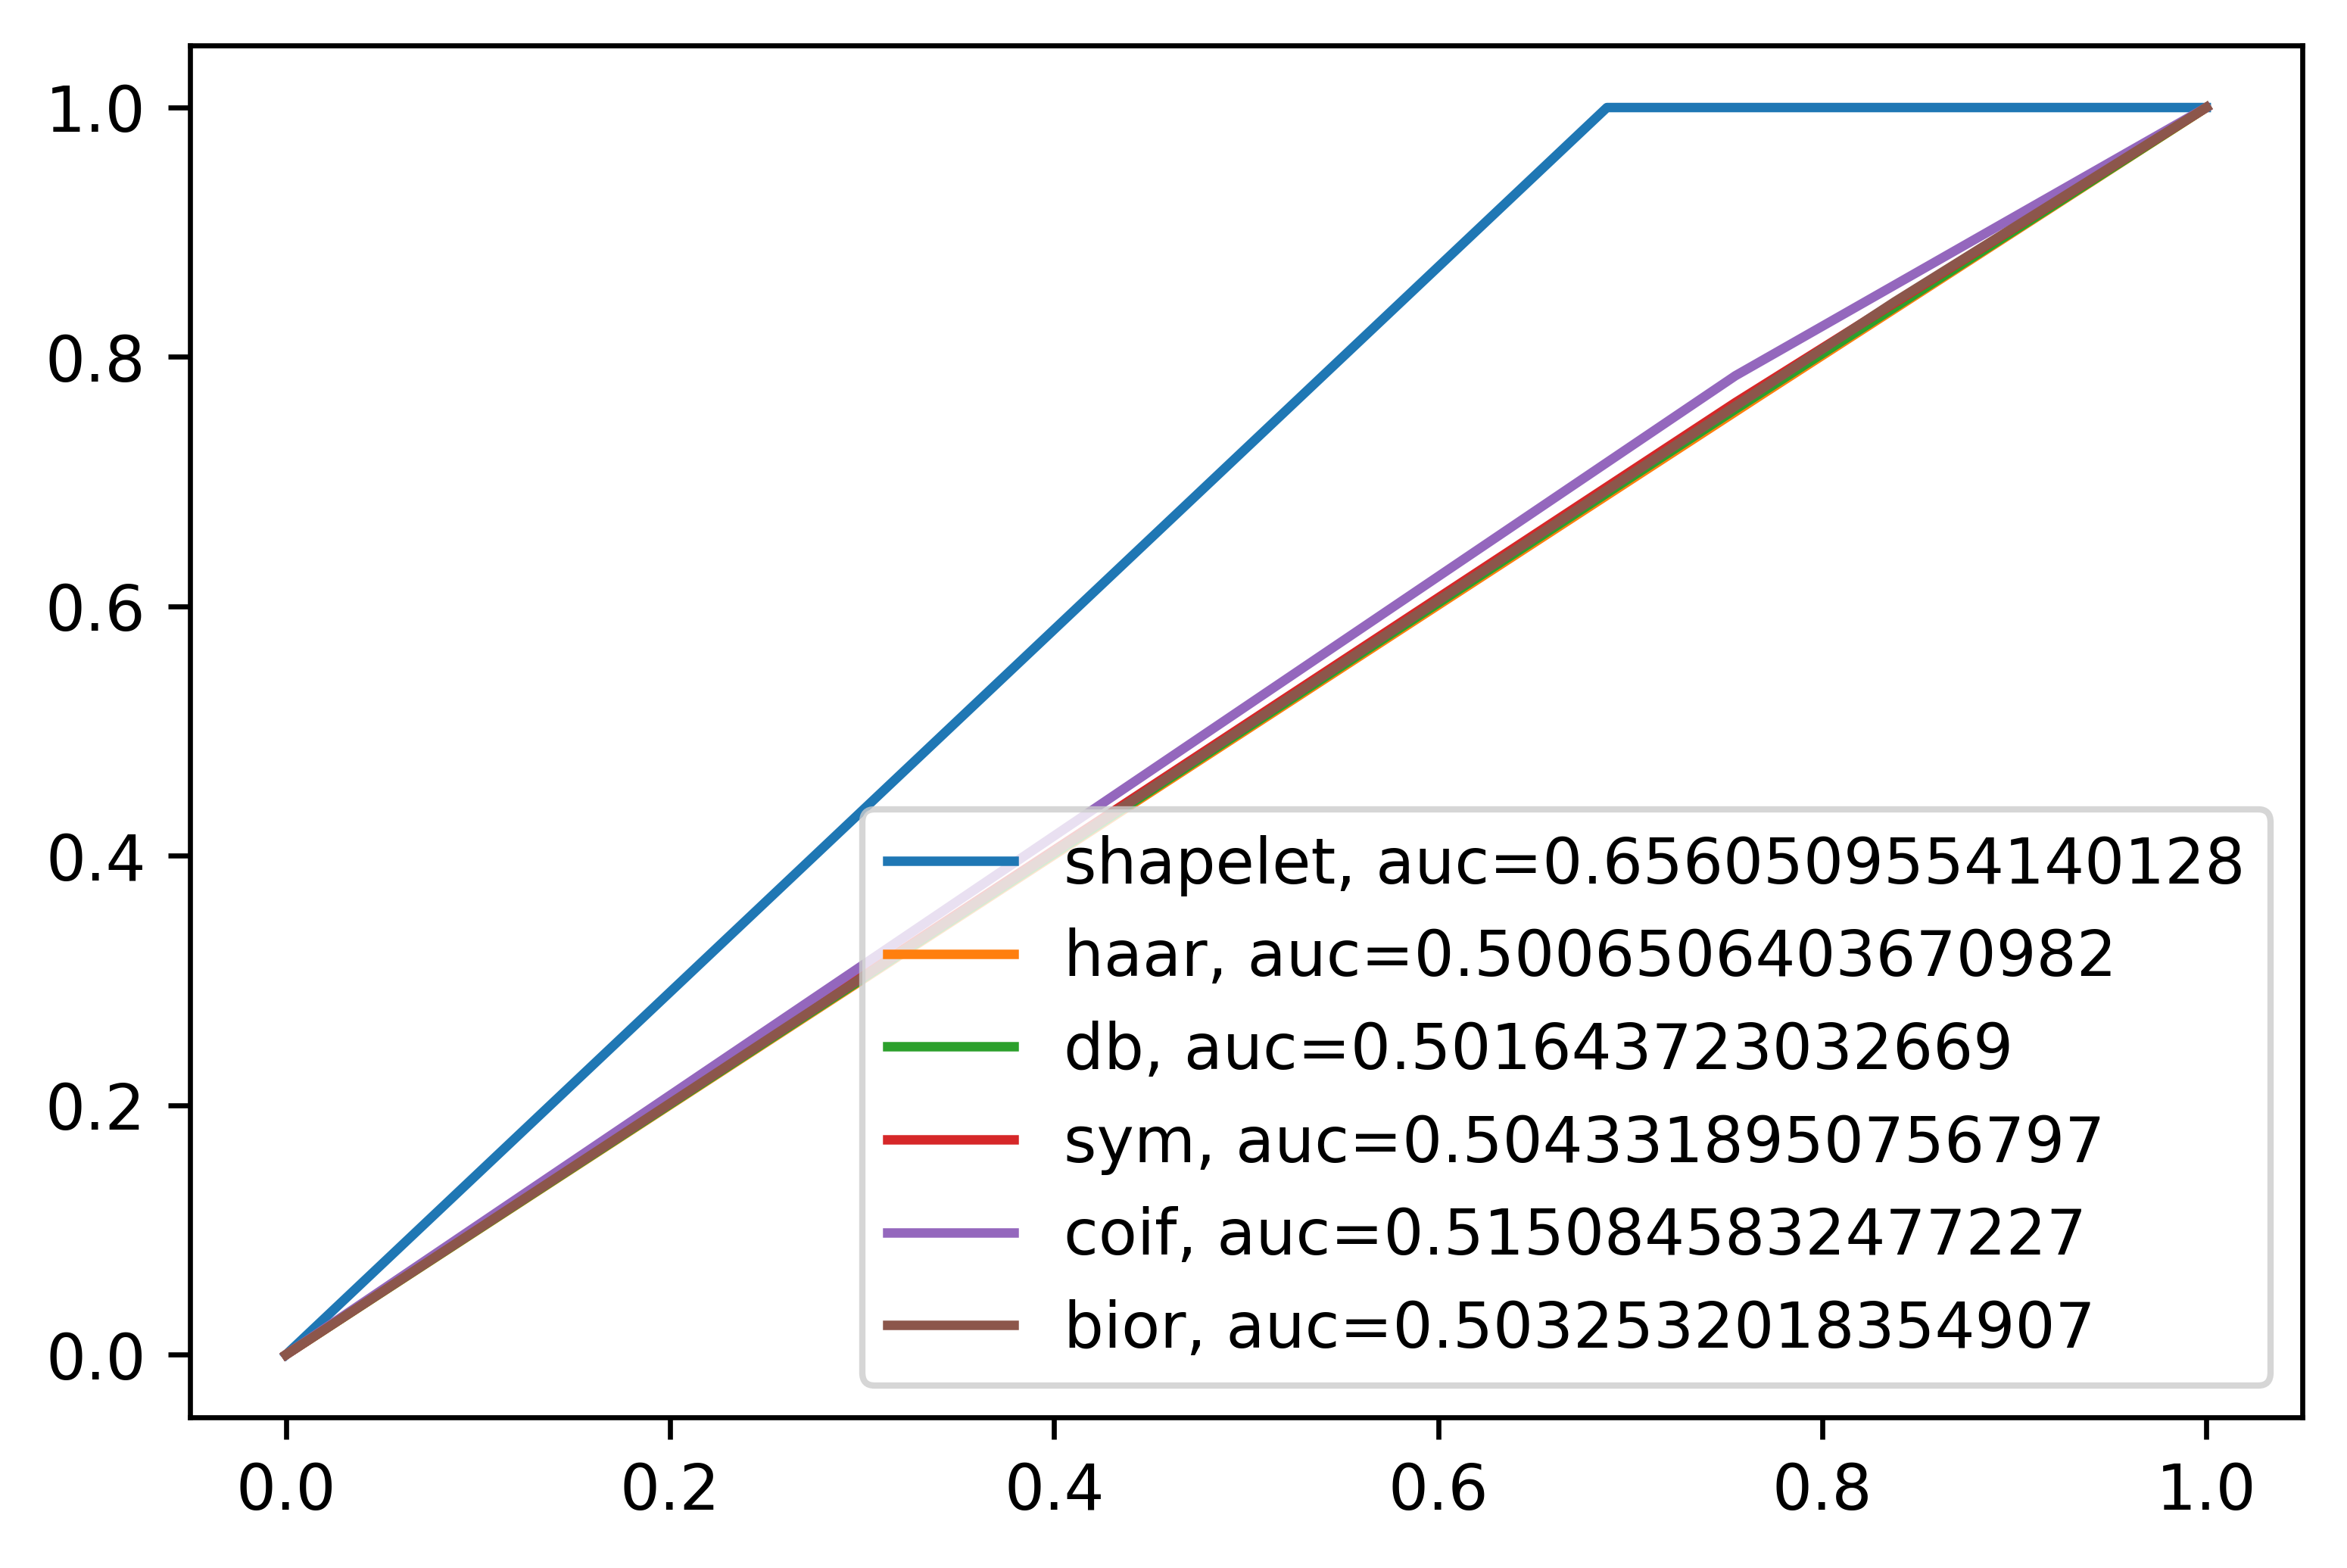
\includegraphics[scale=0.5]{Graphics/roc-th-06.png}}
	\caption{Matriz de confusión y curva ROC. En este ejemplo se tomó como umbral $th=0.60$ y un patrón de longitud 17.} \label{fig:1d-experiment-060}
\end{figure}

\begin{figure}
	\centering
	\subfigure[Matriz de confusión]{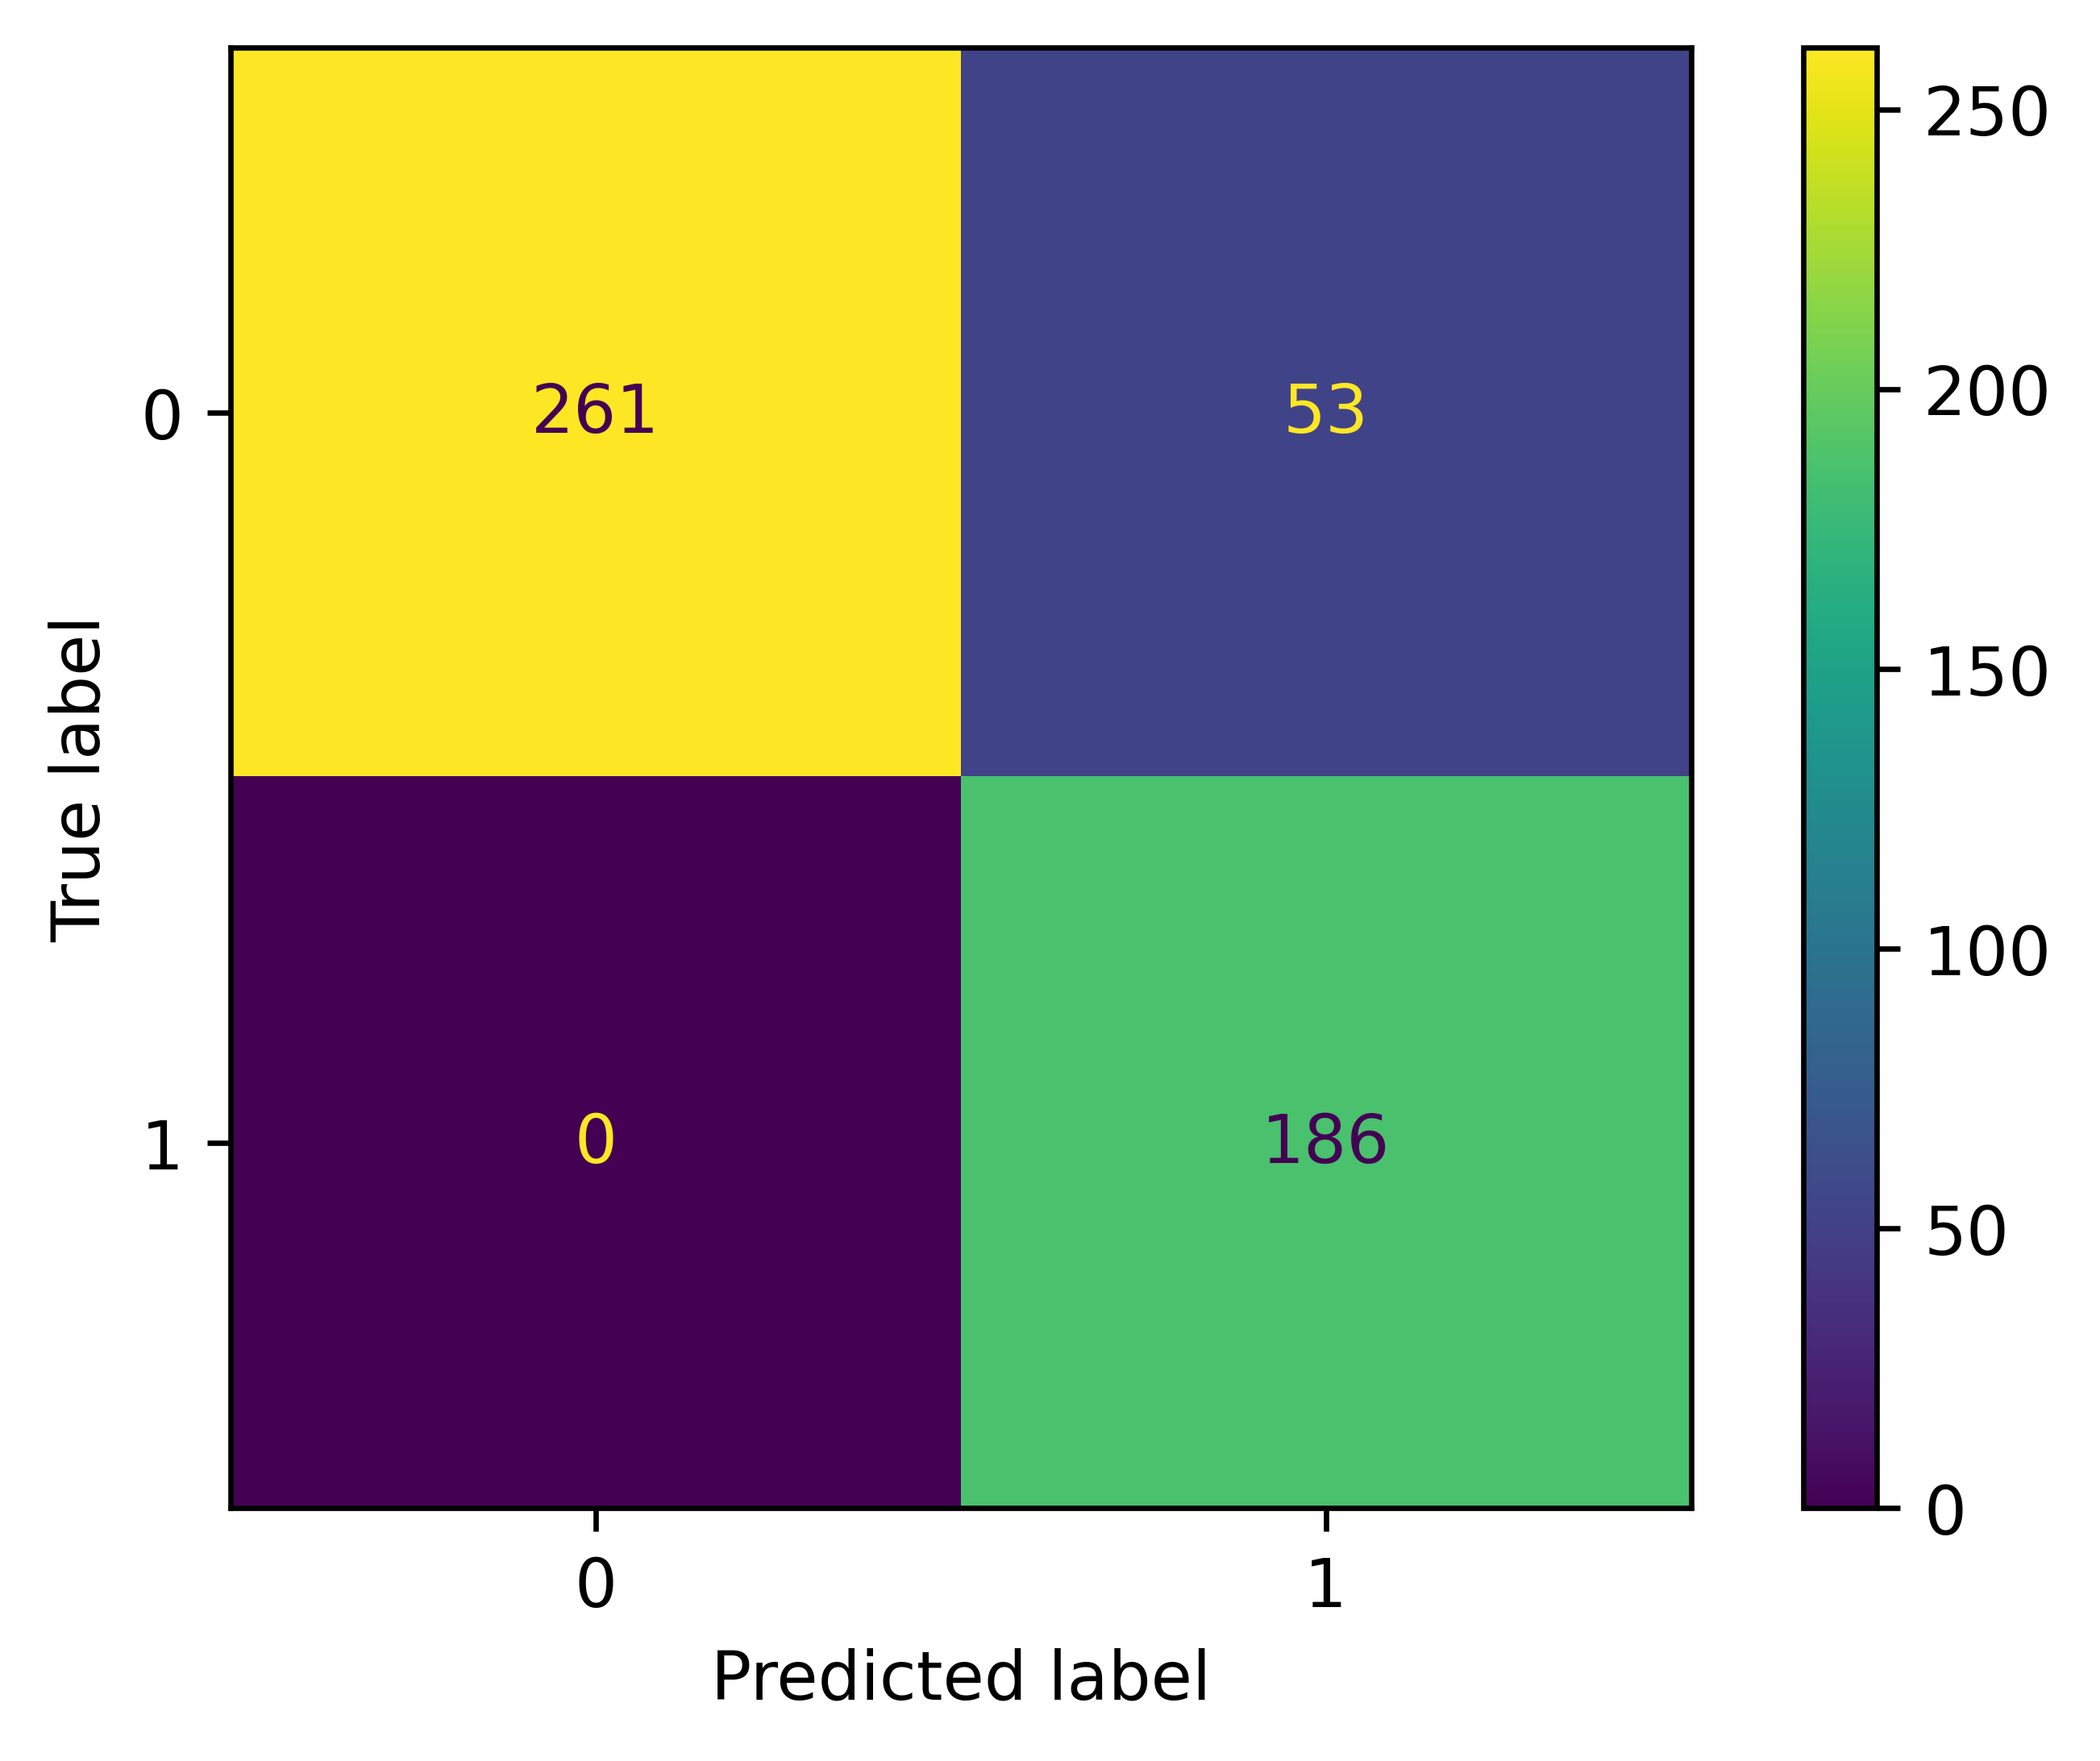
\includegraphics[scale=0.5]{Graphics/cm-th-085.png}}
	\subfigure[Curva ROC]{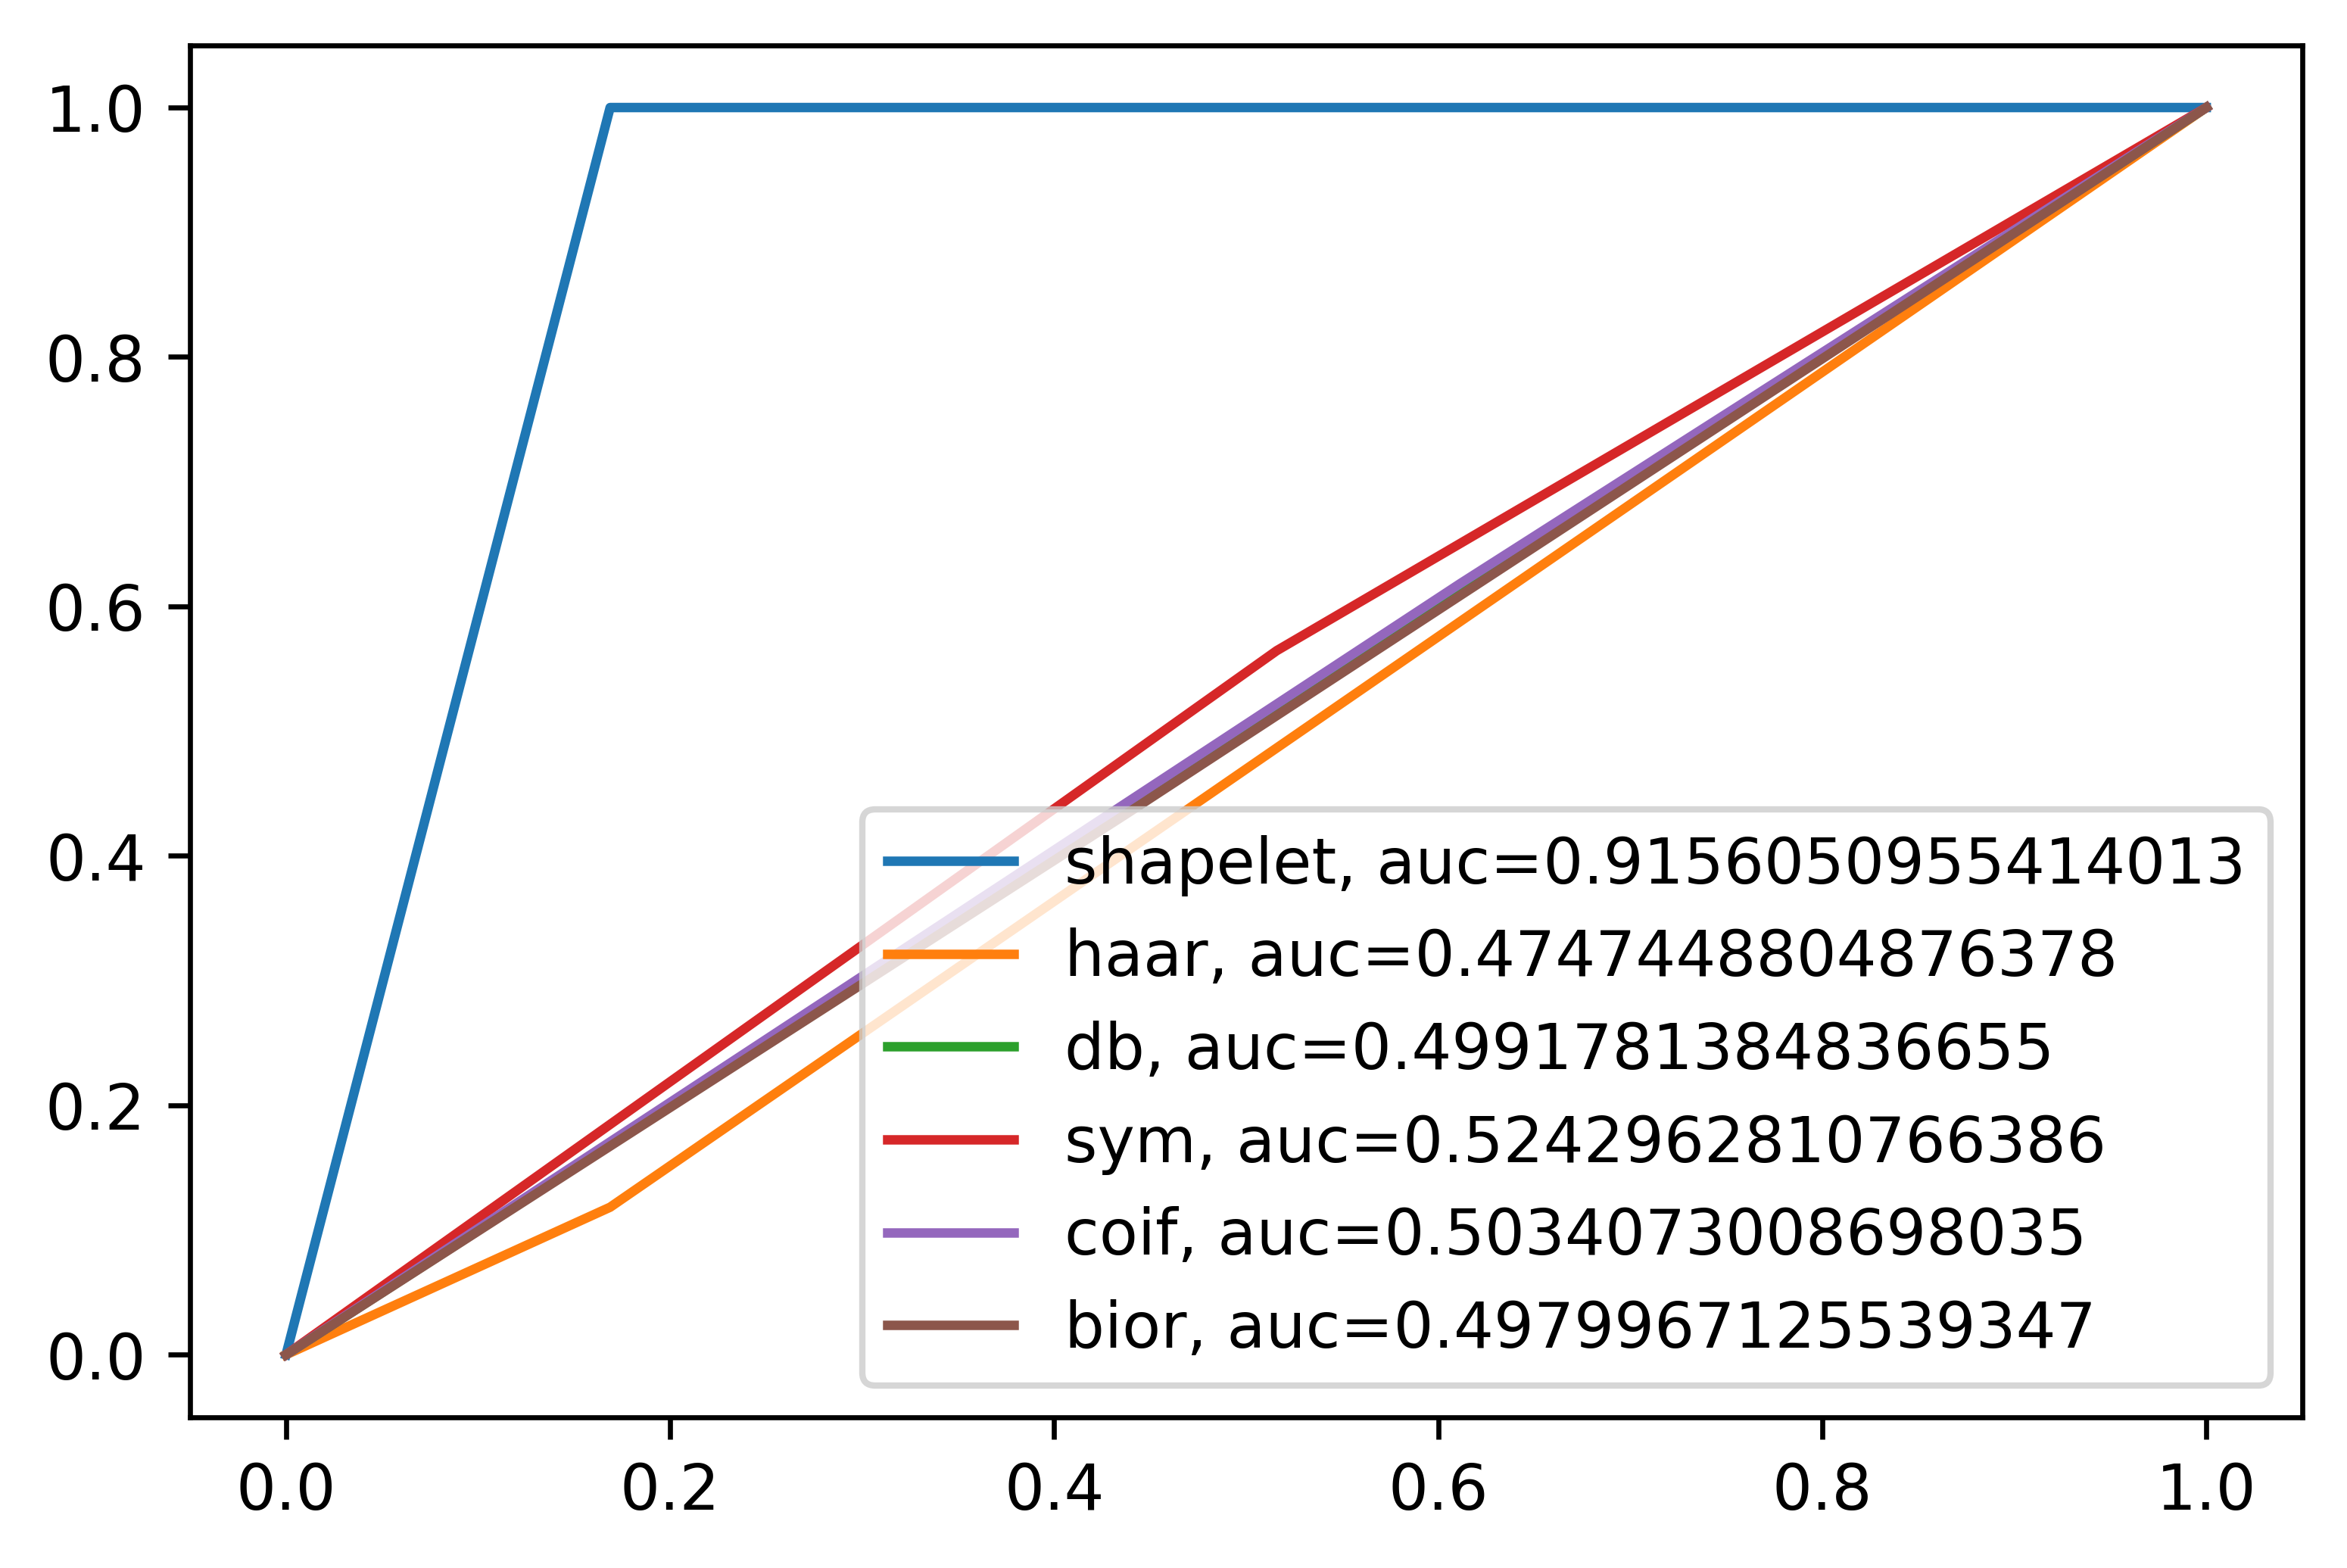
\includegraphics[scale=0.5]{Graphics/roc-th-085.png}}
	\caption{Matriz de confusión y curva ROC. En este ejemplo se tomó como umbral $th=0.85$ y un patrón de longitud 17.} \label{fig:1d-experiment-085}
\end{figure}

\begin{figure}
	\centering
	\subfigure[Matriz de confusión]{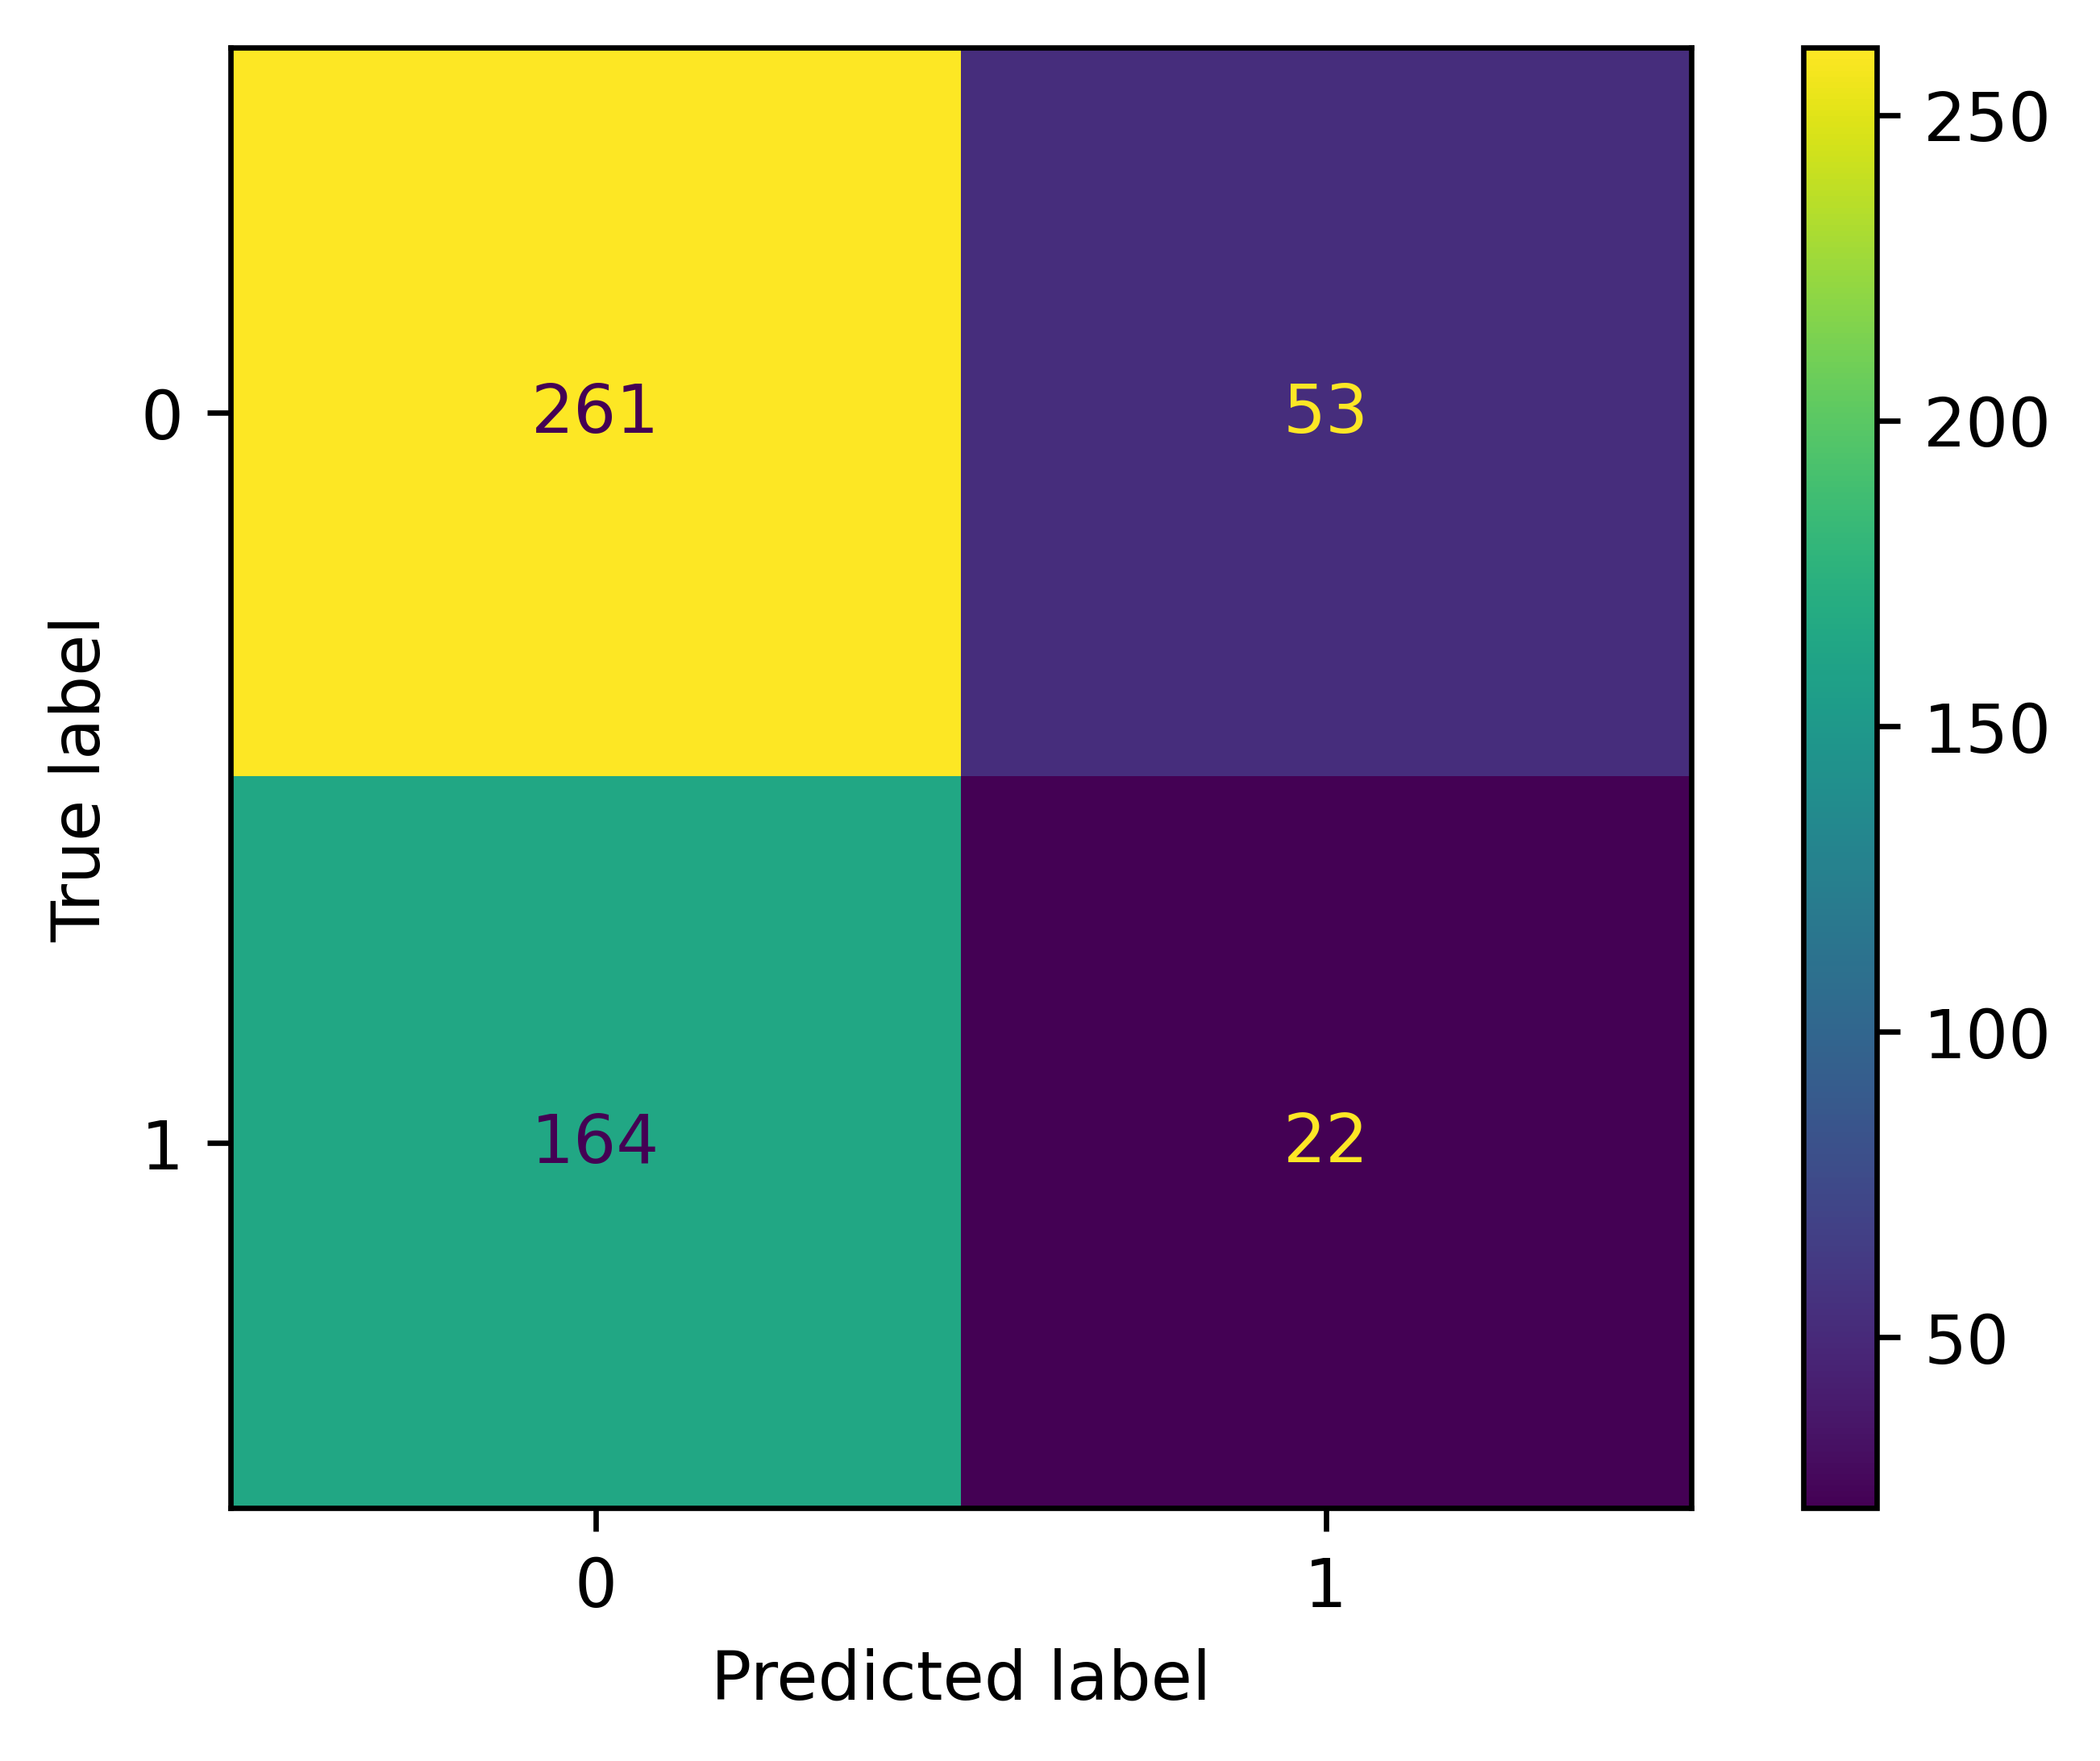
\includegraphics[scale=0.5]{Graphics/cm-th-098.png}}
	\subfigure[Curva ROC]{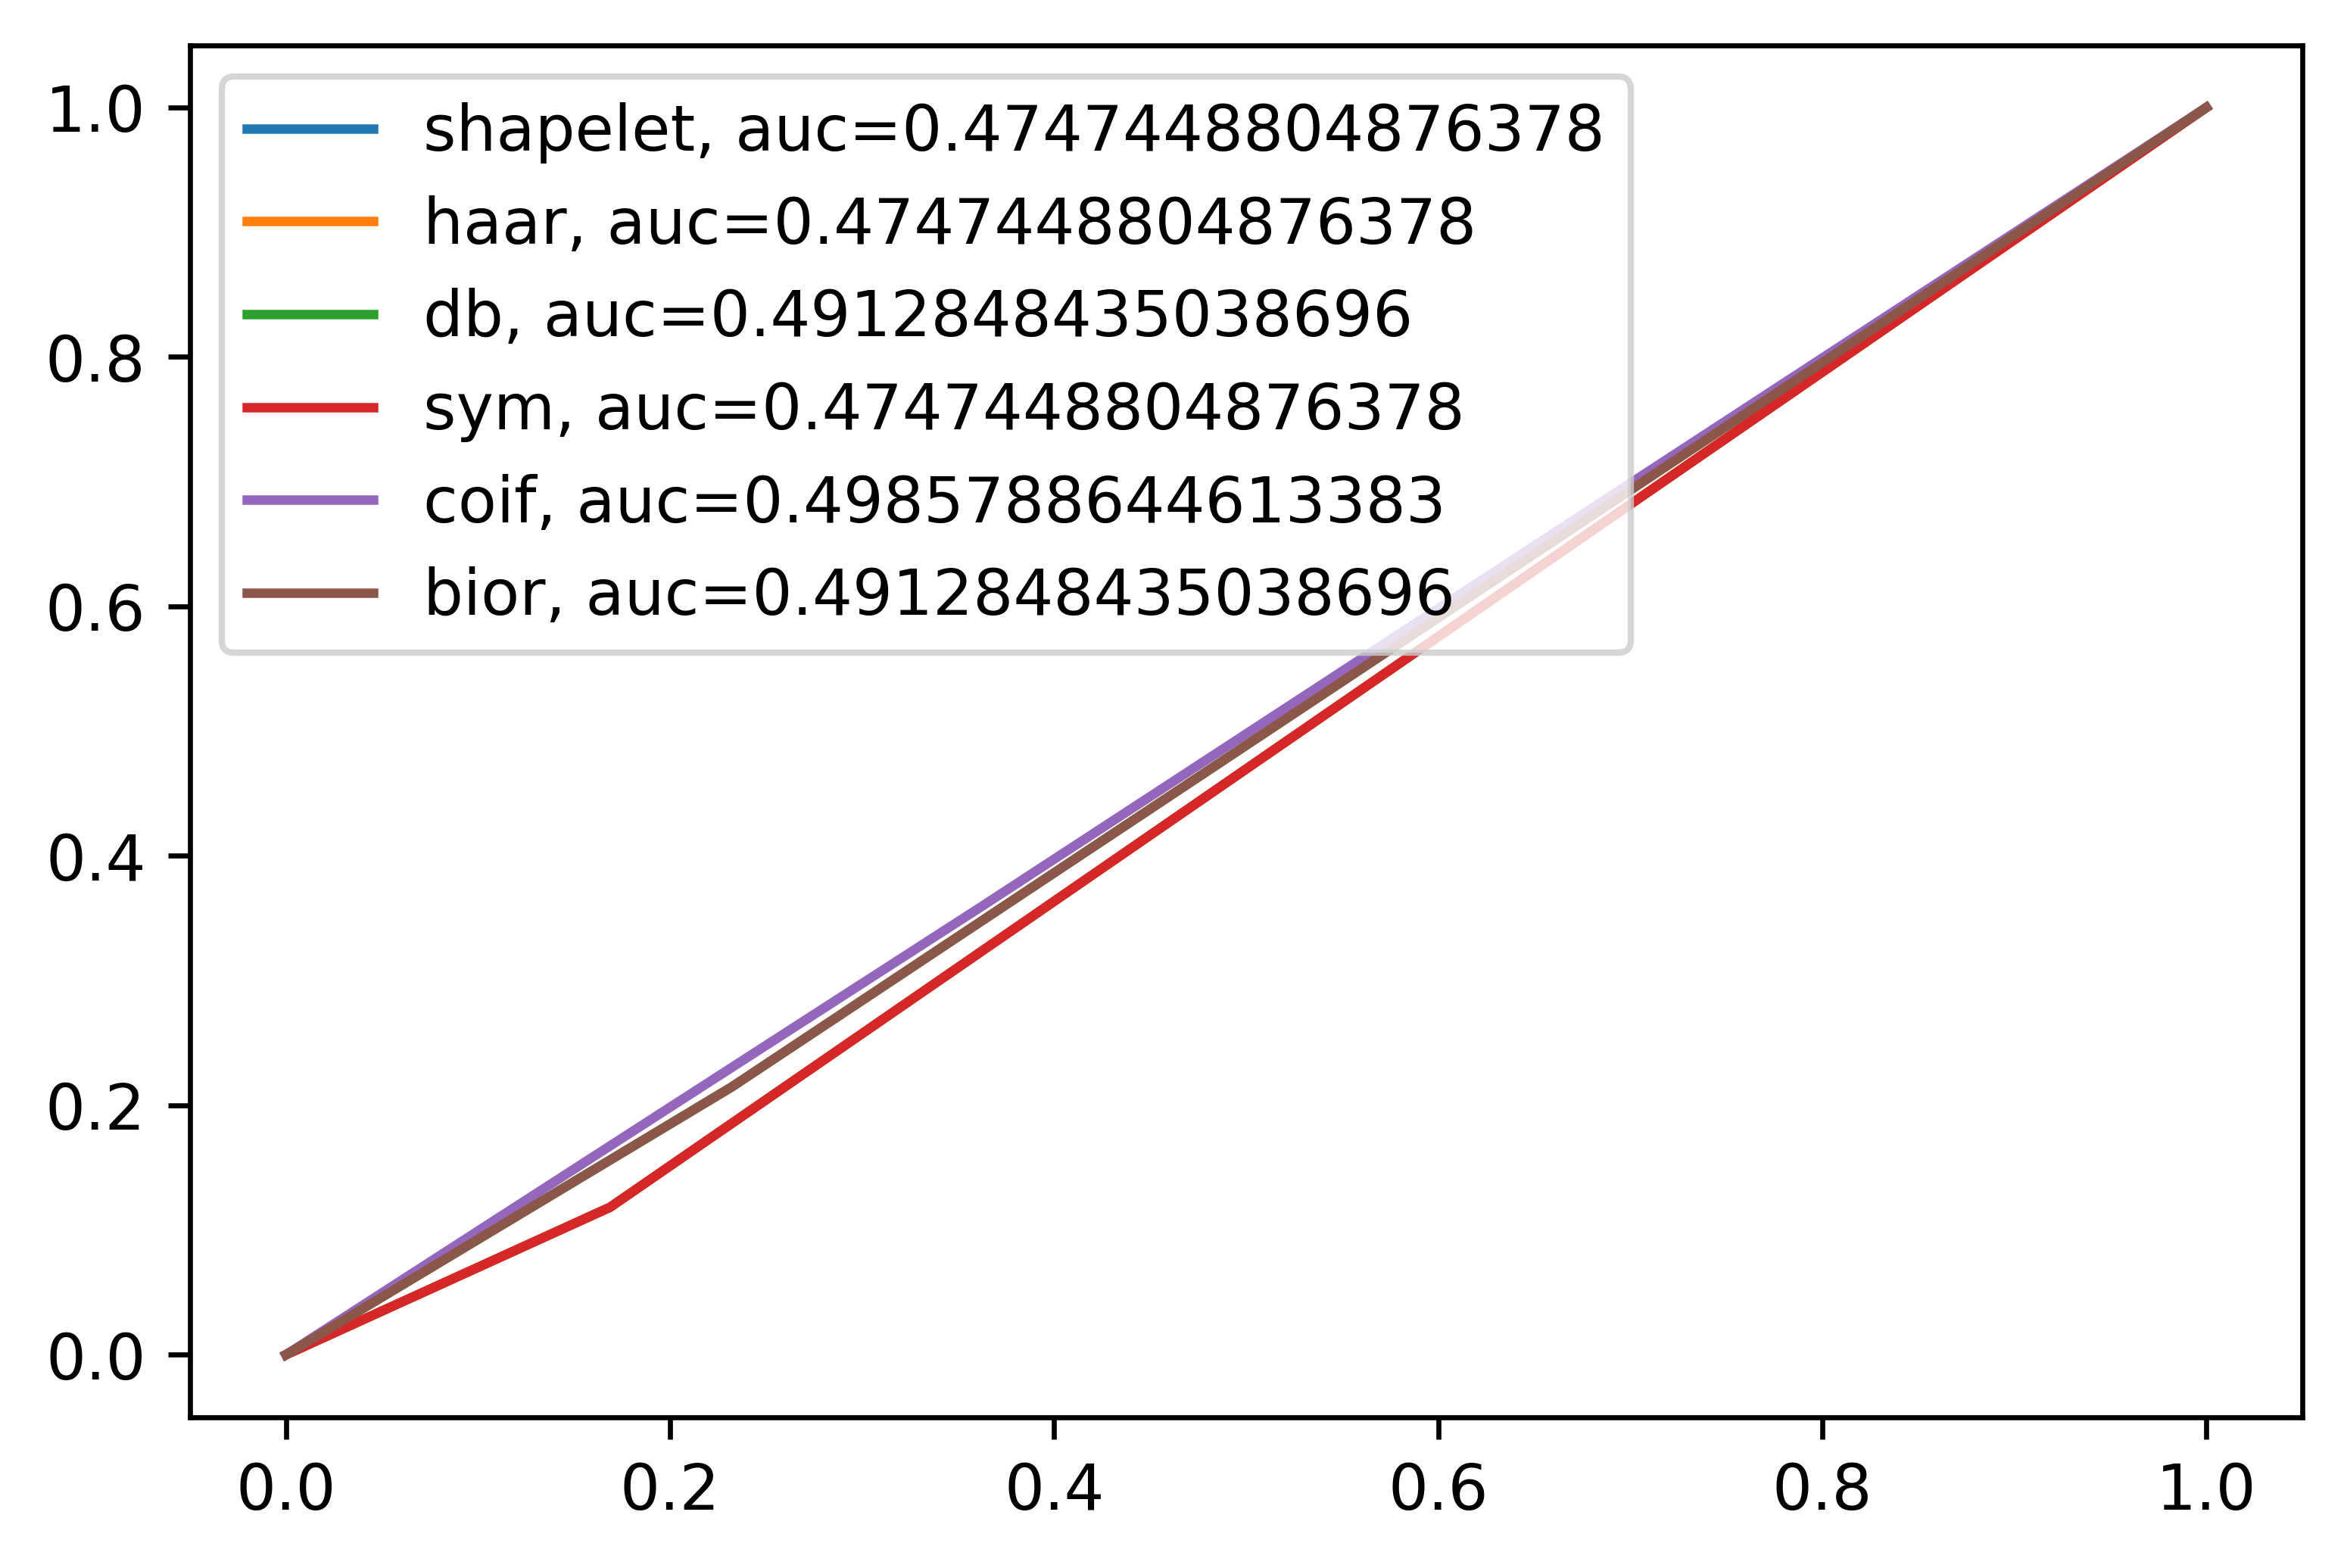
\includegraphics[scale=0.5]{Graphics/roc-th-098.png}}
	\caption{Matriz de confusión y curva ROC. En este ejemplo se tomó como umbral $th=0.98$ y un patrón de longitud 17.} \label{fig:1d-experiment-098}
\end{figure}

La selección del umbral $th$ para la medida $\mathbb{S}$ también es importante.
Las figuras \ref{fig:1d-experiment-060}, \ref{fig:1d-experiment-060} y \ref{fig:1d-experiment-098} muestran los resultados 
sobre un mismo patron constituido por 17 muestras, pero variando el umbral $th$. El método numérico para la solución es el
mismo: Levenberg-Marquardt.

Seleccionando un umbral $th=0.6$, permite al algoritmo sacarle provecho a su capacidad de detectar el patrón. Sin embargo,
sigue habiendo una gran cantidad de falsos positivos. Si se aumenta este umbral a $th=0.85$ este número
disminuye considerablemente, pues de 216 pasa a ser tan solo 53. Como consecuencia de esto, el área debajo de la curva
(\textit{auc}) llega a alcanzar $0.90$, lo cual es un resultado sumamente bueno para un clasificador binario.

Si se sigue aumentando el umbral, esta vez a $0.98$, los resultados cambian drásticamente. La \textit{shapelet} no
se comporta para nada distinto al resto de las wavelets. Aunque teóricamente un valor igual a cero en $\mathbb{S}$ indica
la detección exacta del patrón, siempre existe un error durante el cálculo del filtro $q$ que impide que esto sea
cierto en la práctica. Por este motivo, poner el umbral de detección demasiado alto empeora los resultados.
Por lo tanto, un valor entre $0.6$ (valor que recomiendan en \cite{Guido2018}) y $0.90$ se considera idóneo.


\begin{figure}
	\centering
	\subfigure[Patrón]{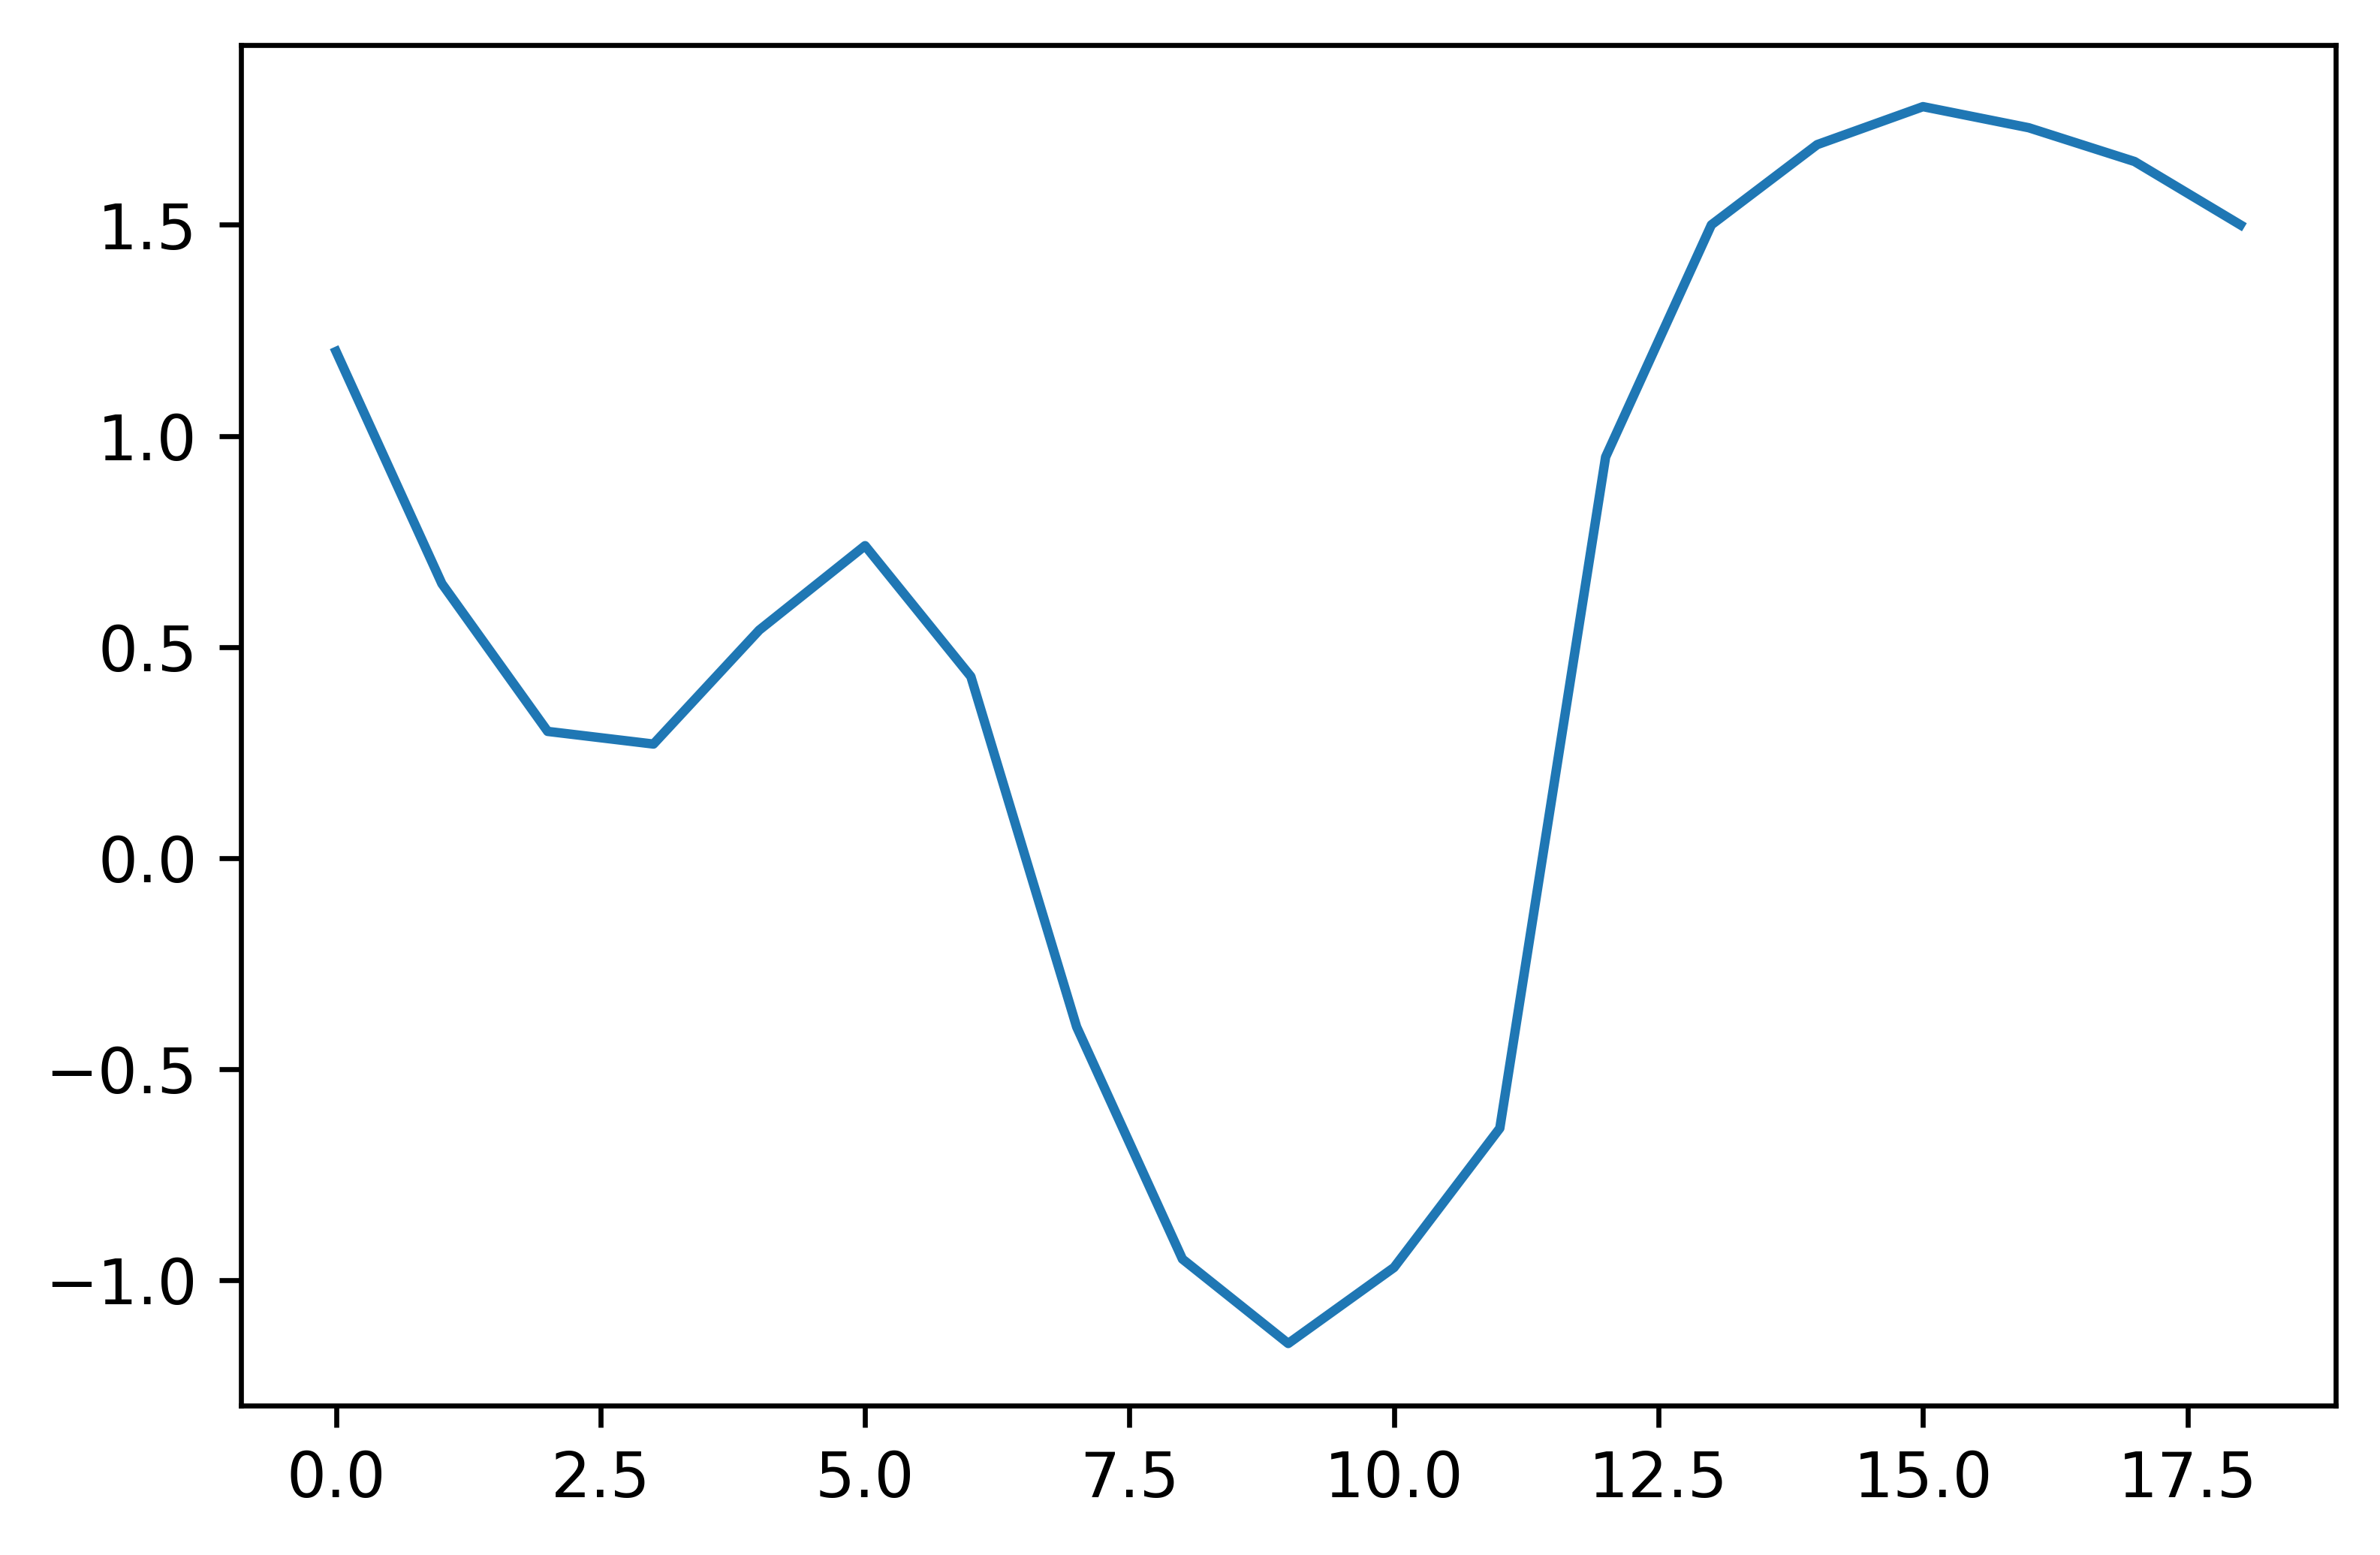
\includegraphics[scale=0.5]{Graphics/success-example-pattern.png}}
	\subfigure[Señal con patrón insertado]{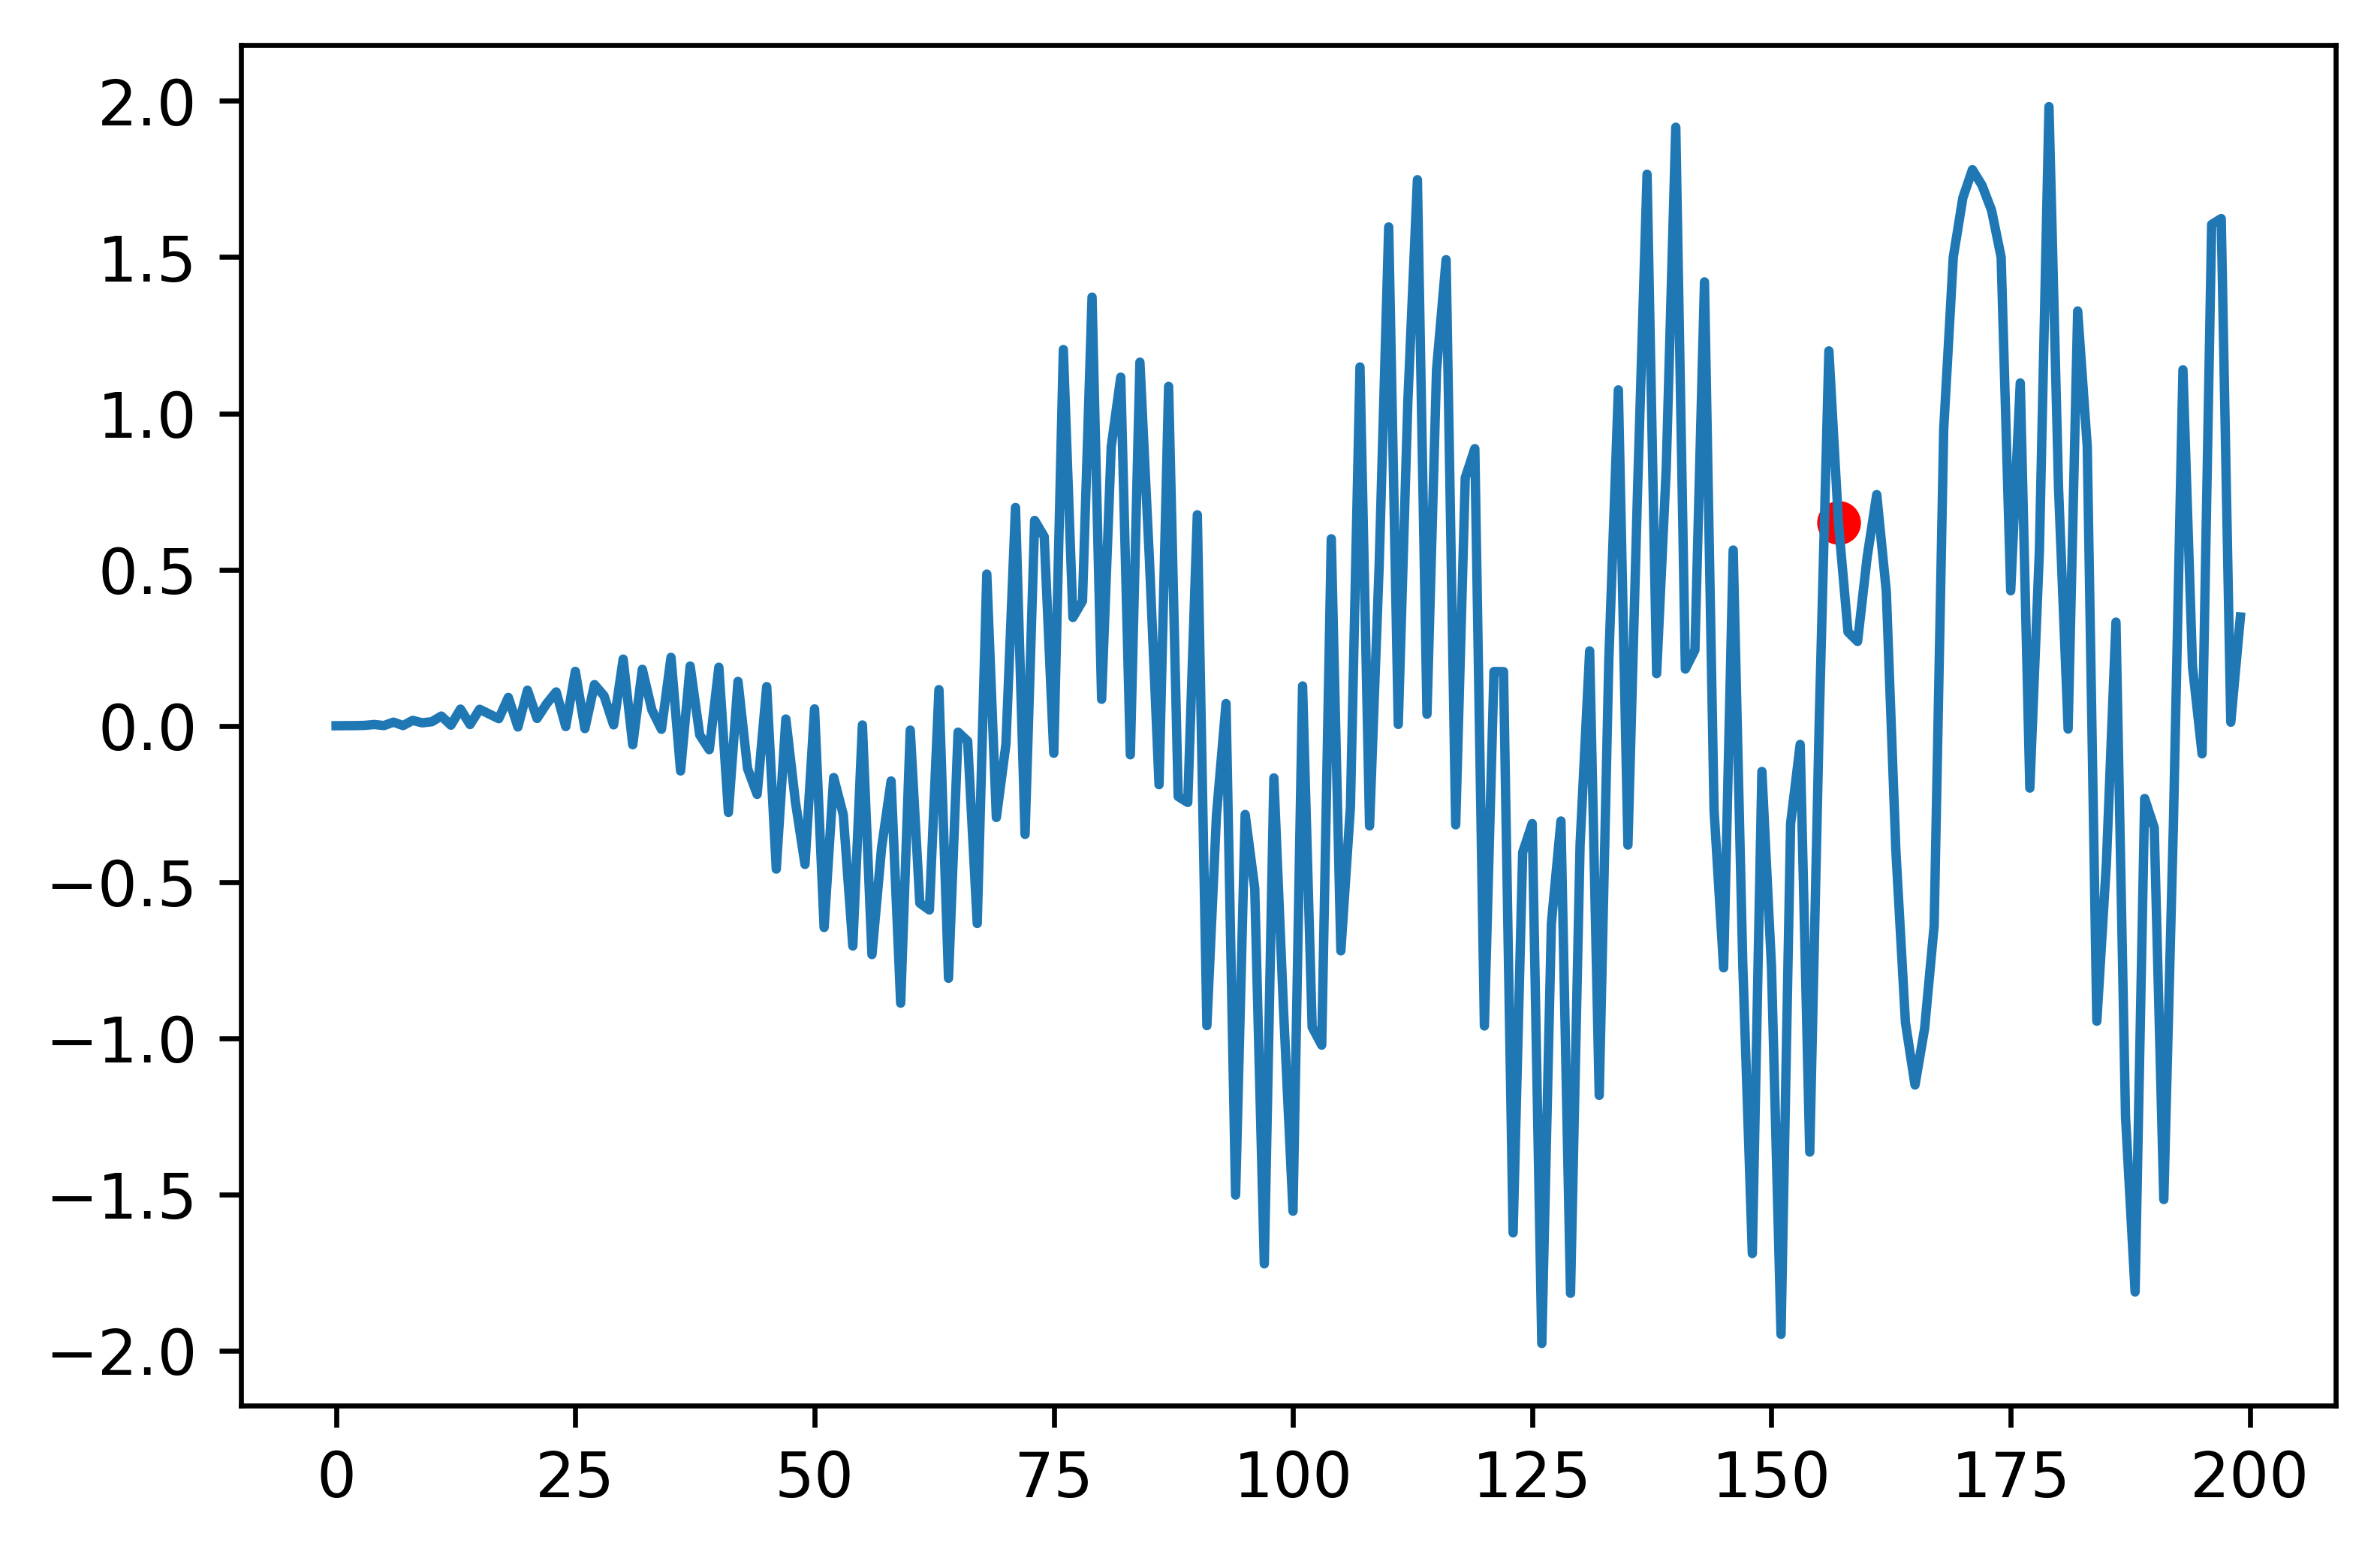
\includegraphics[scale=0.5]{Graphics/success-example-signal.png}}
	\subfigure[Major shapelet]{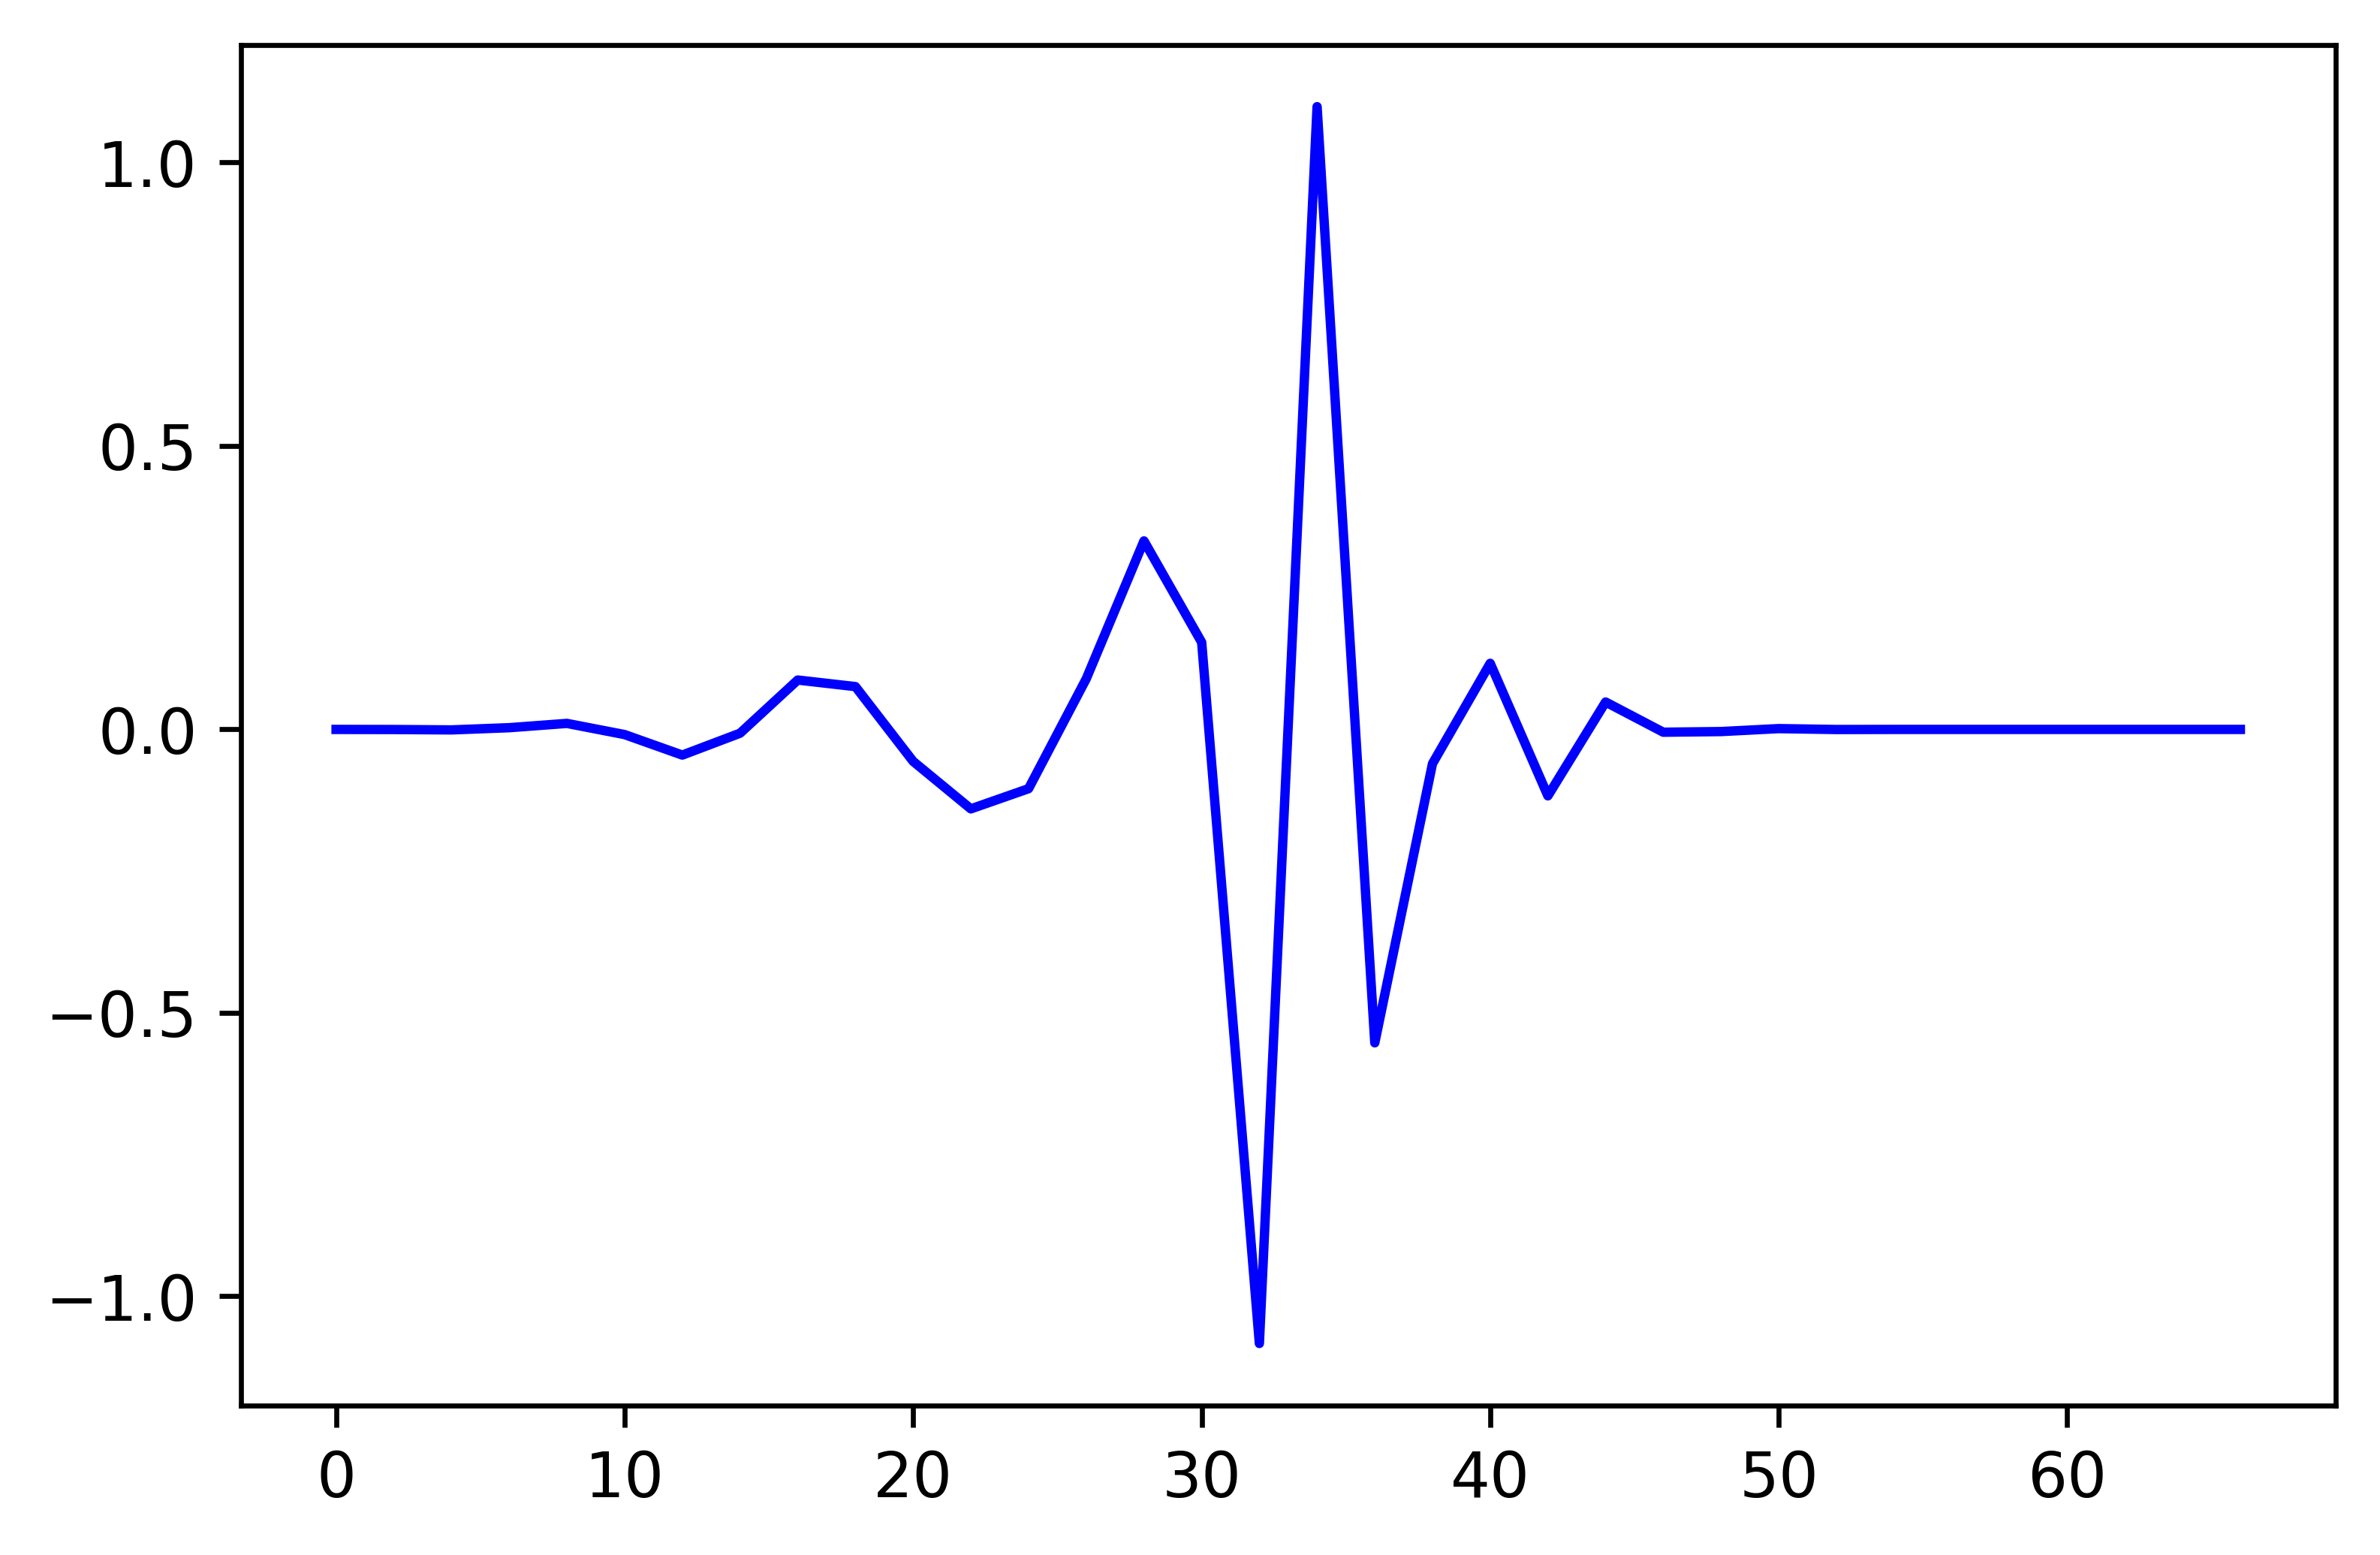
\includegraphics[scale=0.5]{Graphics/success-example-blue-shapelet.png}}
	\subfigure[Minor shapelet]{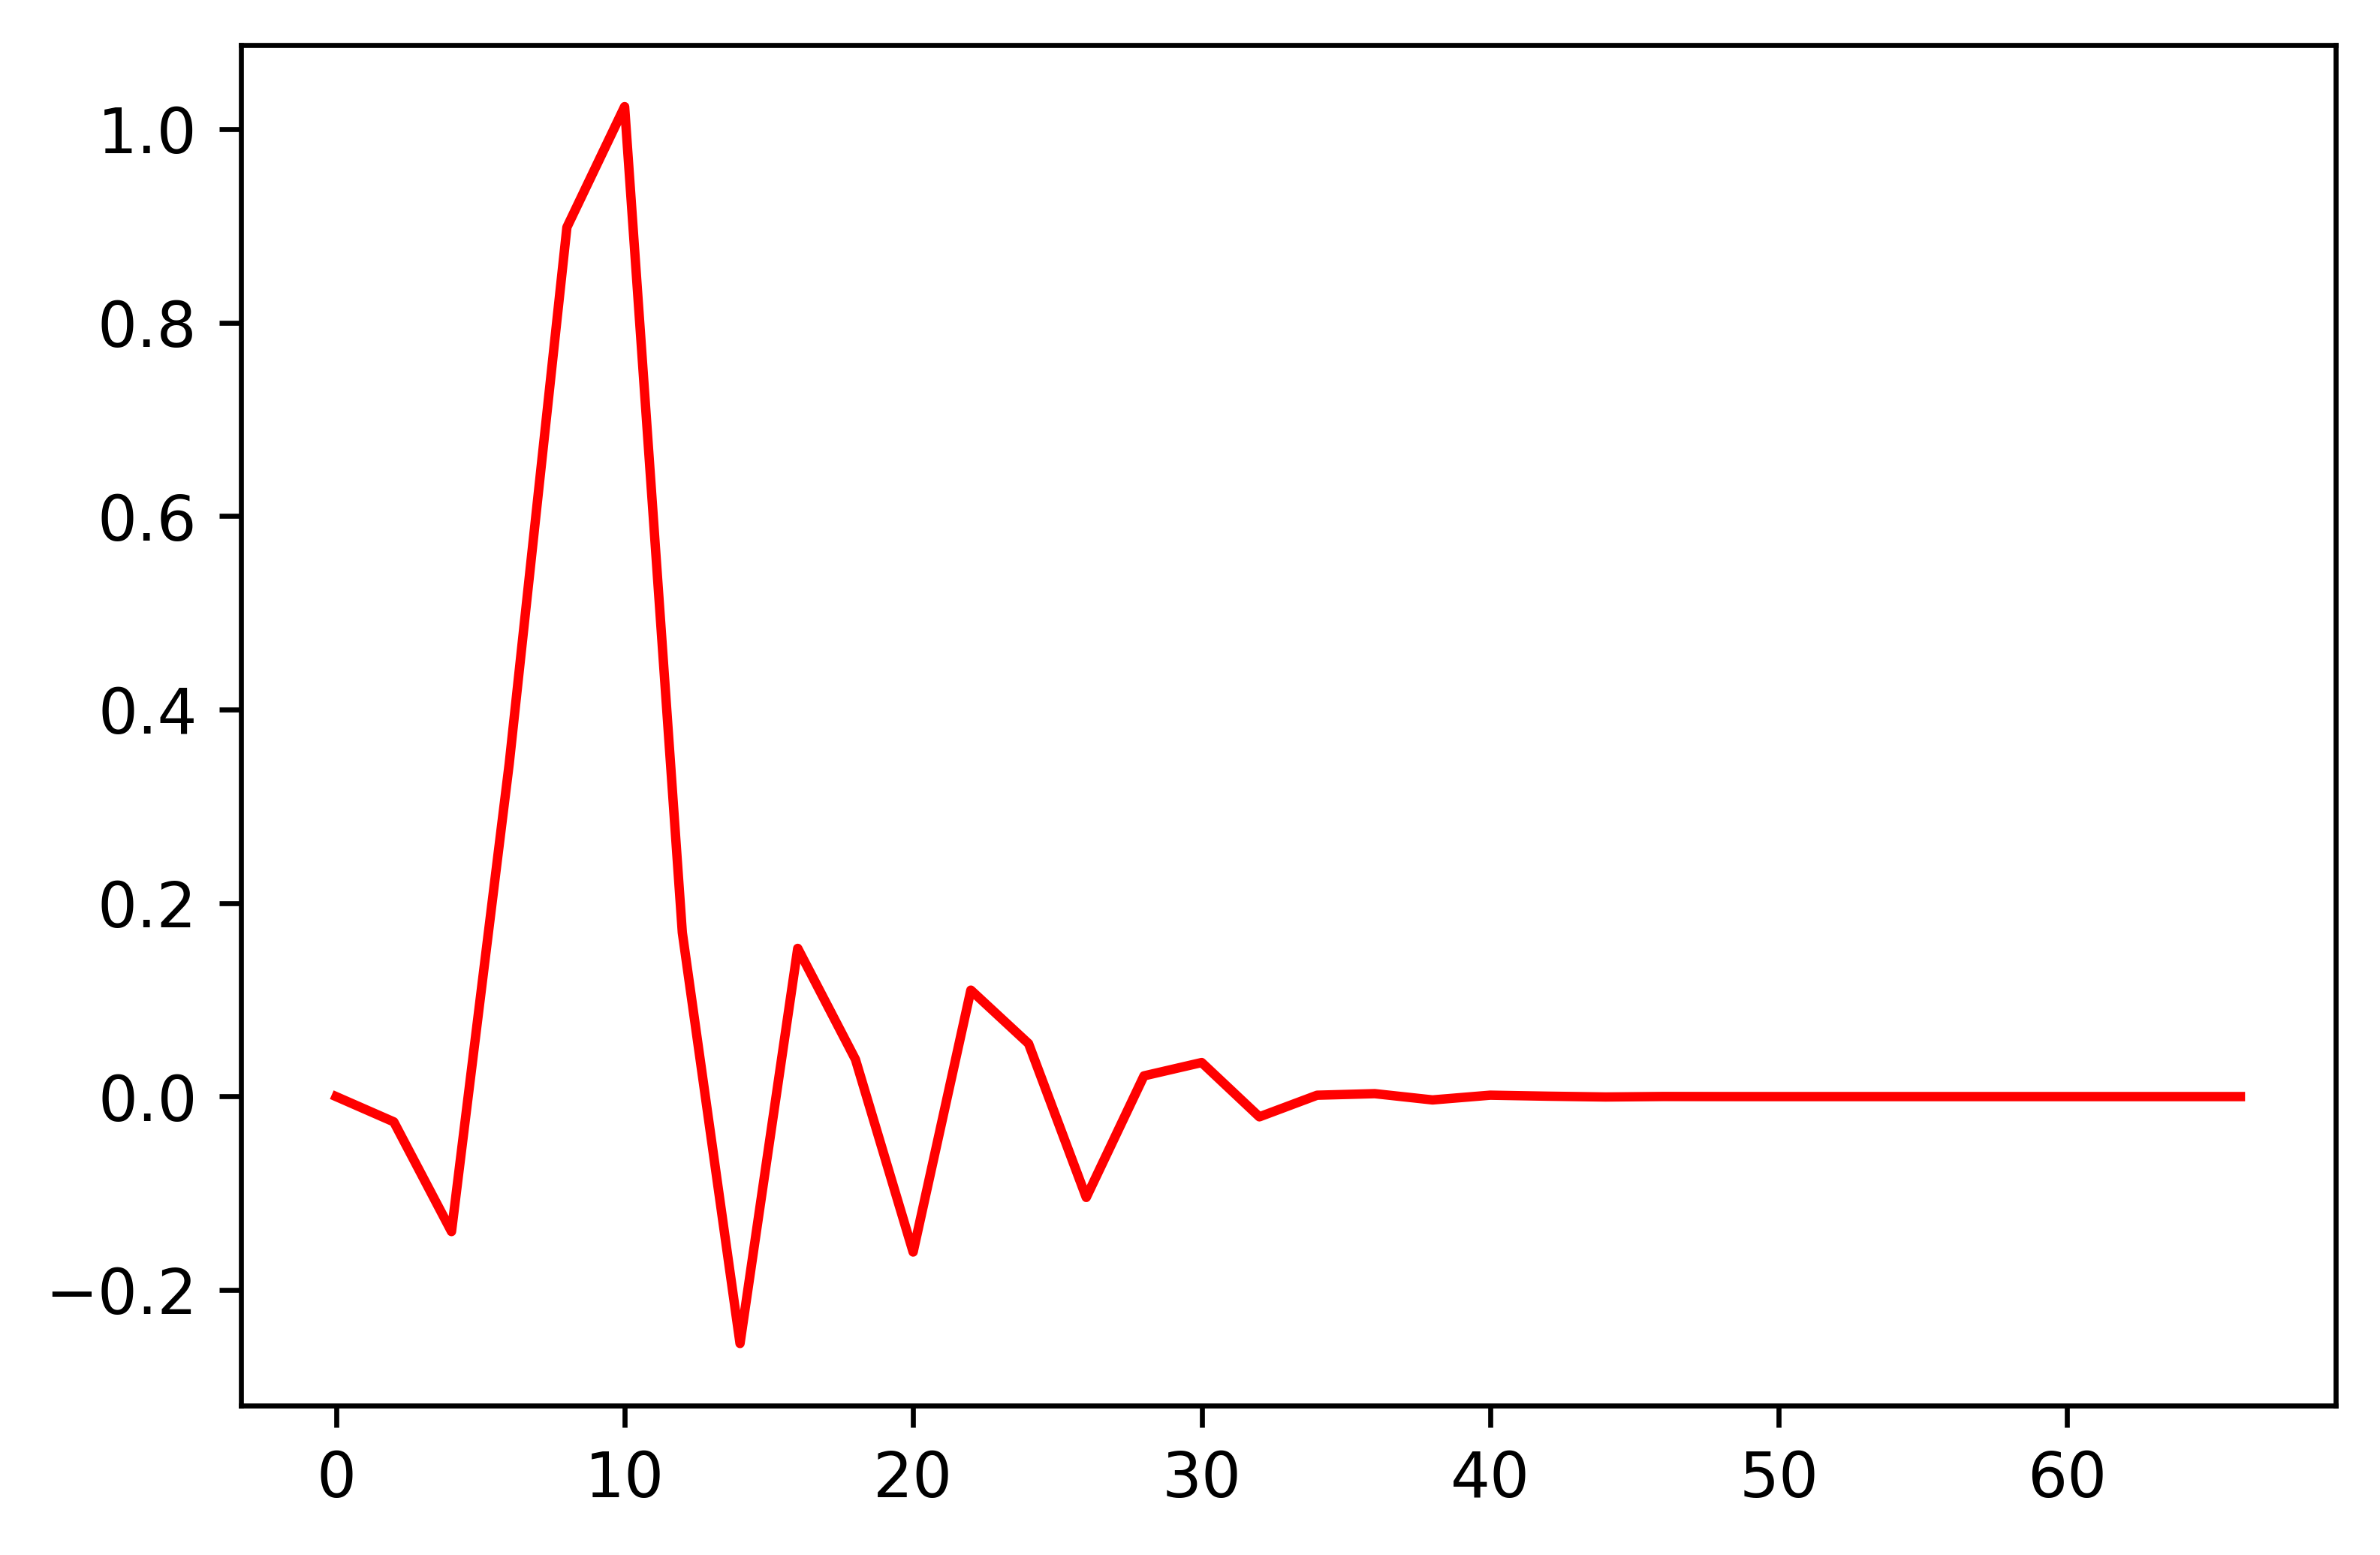
\includegraphics[scale=0.5]{Graphics/success-example-red-shapelet.png}}
	\subfigure[DST-II y medida $\mathbb{S}$]{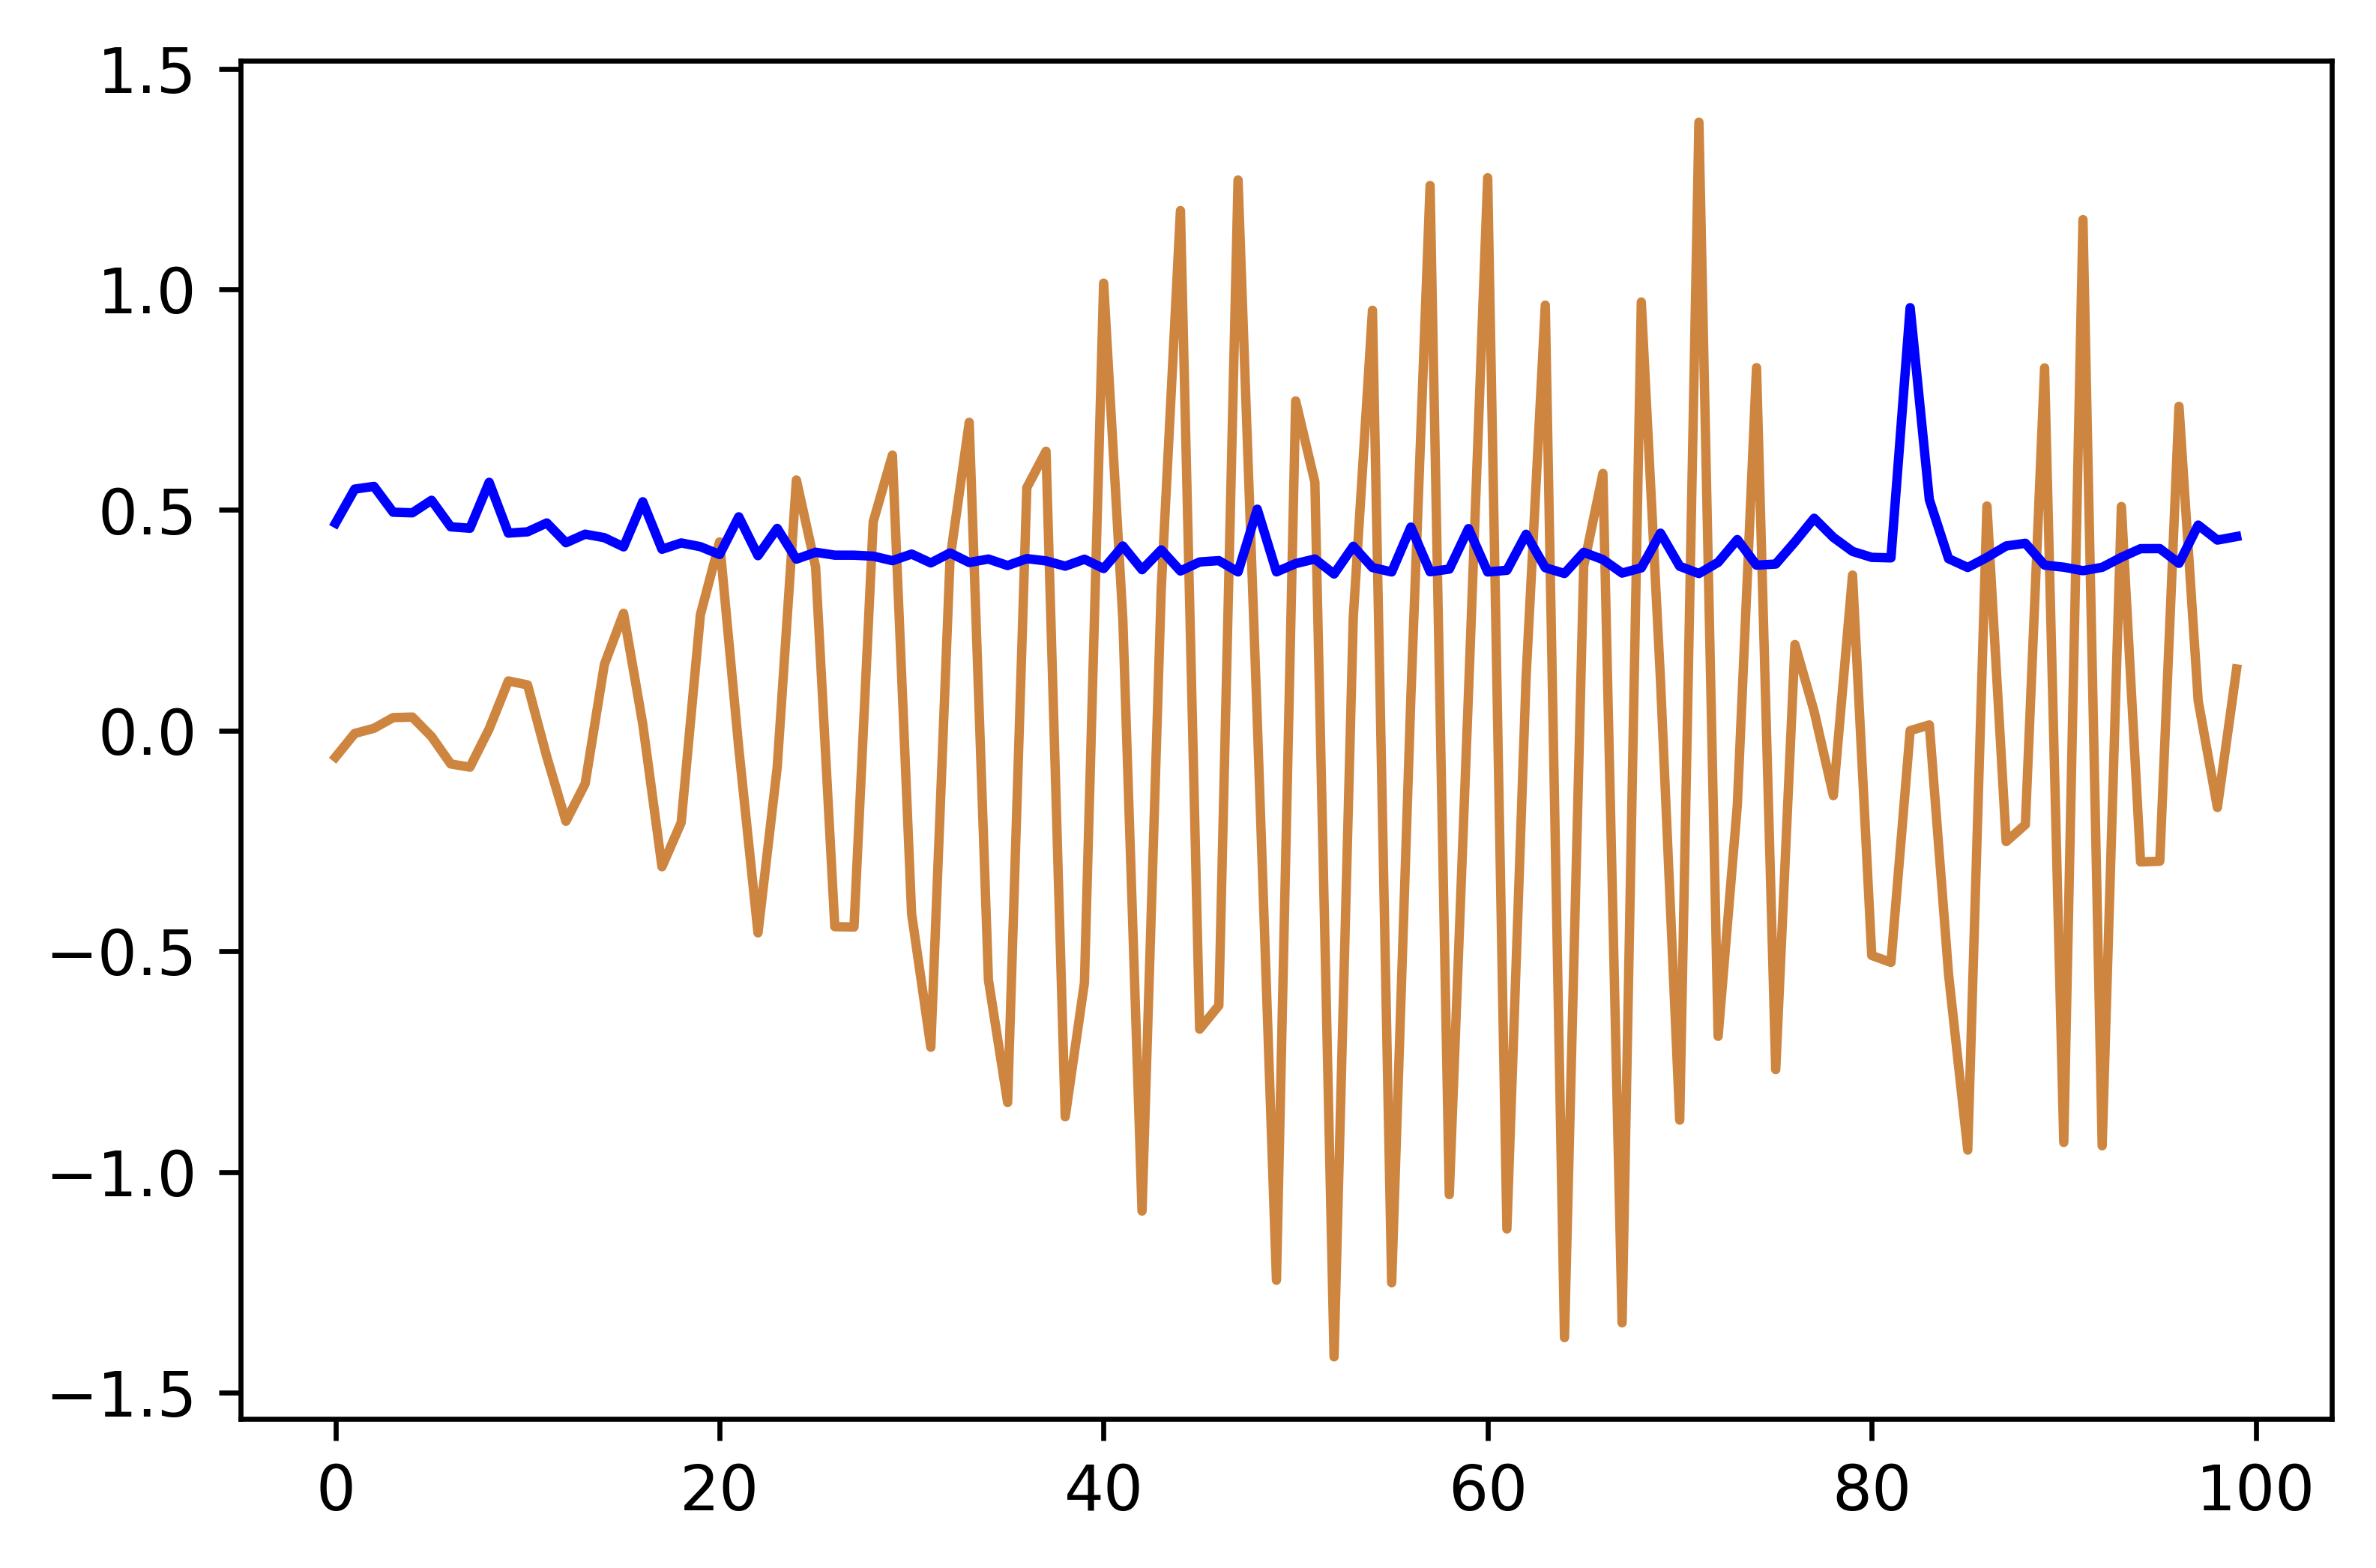
\includegraphics[scale=0.5]{Graphics/success-example-detection.png}}
	\caption{Ejemplo donde el algoritmo logra detectar la posición donde se encuentra el patrón.} \label{fig:success-example-experiment}
\end{figure}

\begin{figure}
	\centering
	\subfigure[Patrón]{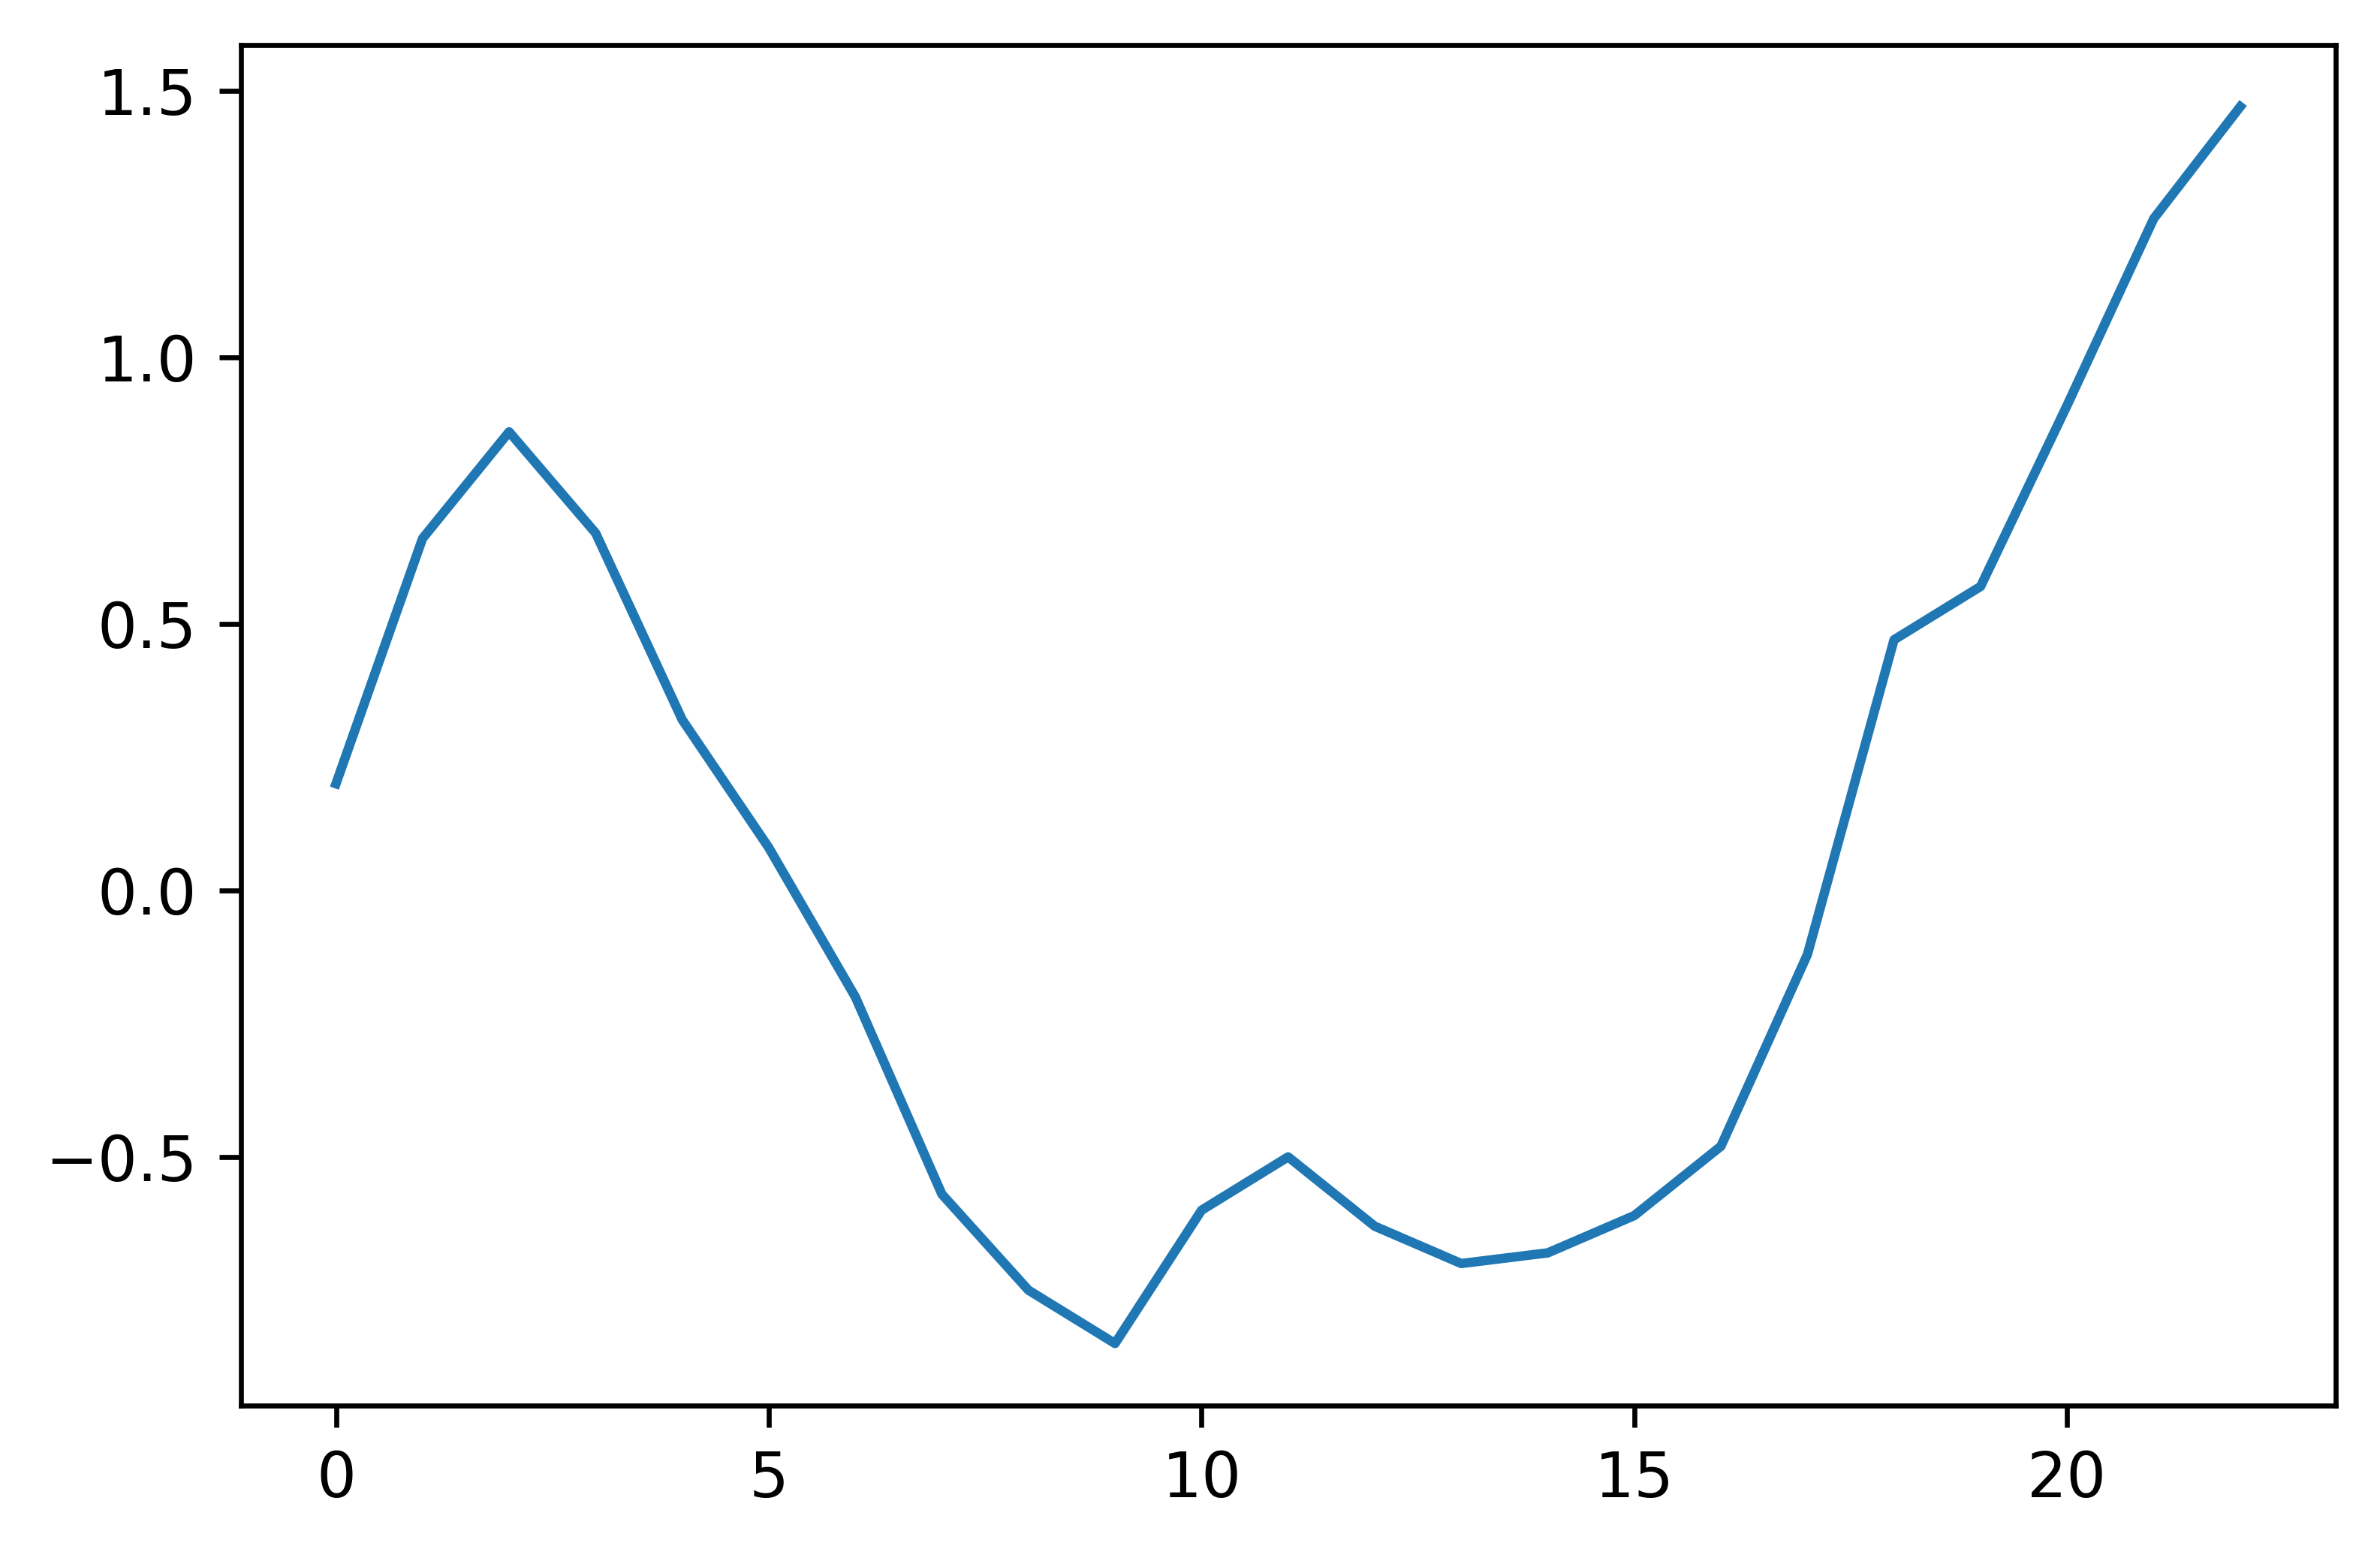
\includegraphics[scale=0.5]{Graphics/failed-example-pattern.png}}
	\subfigure[Señal con patrón insertado]{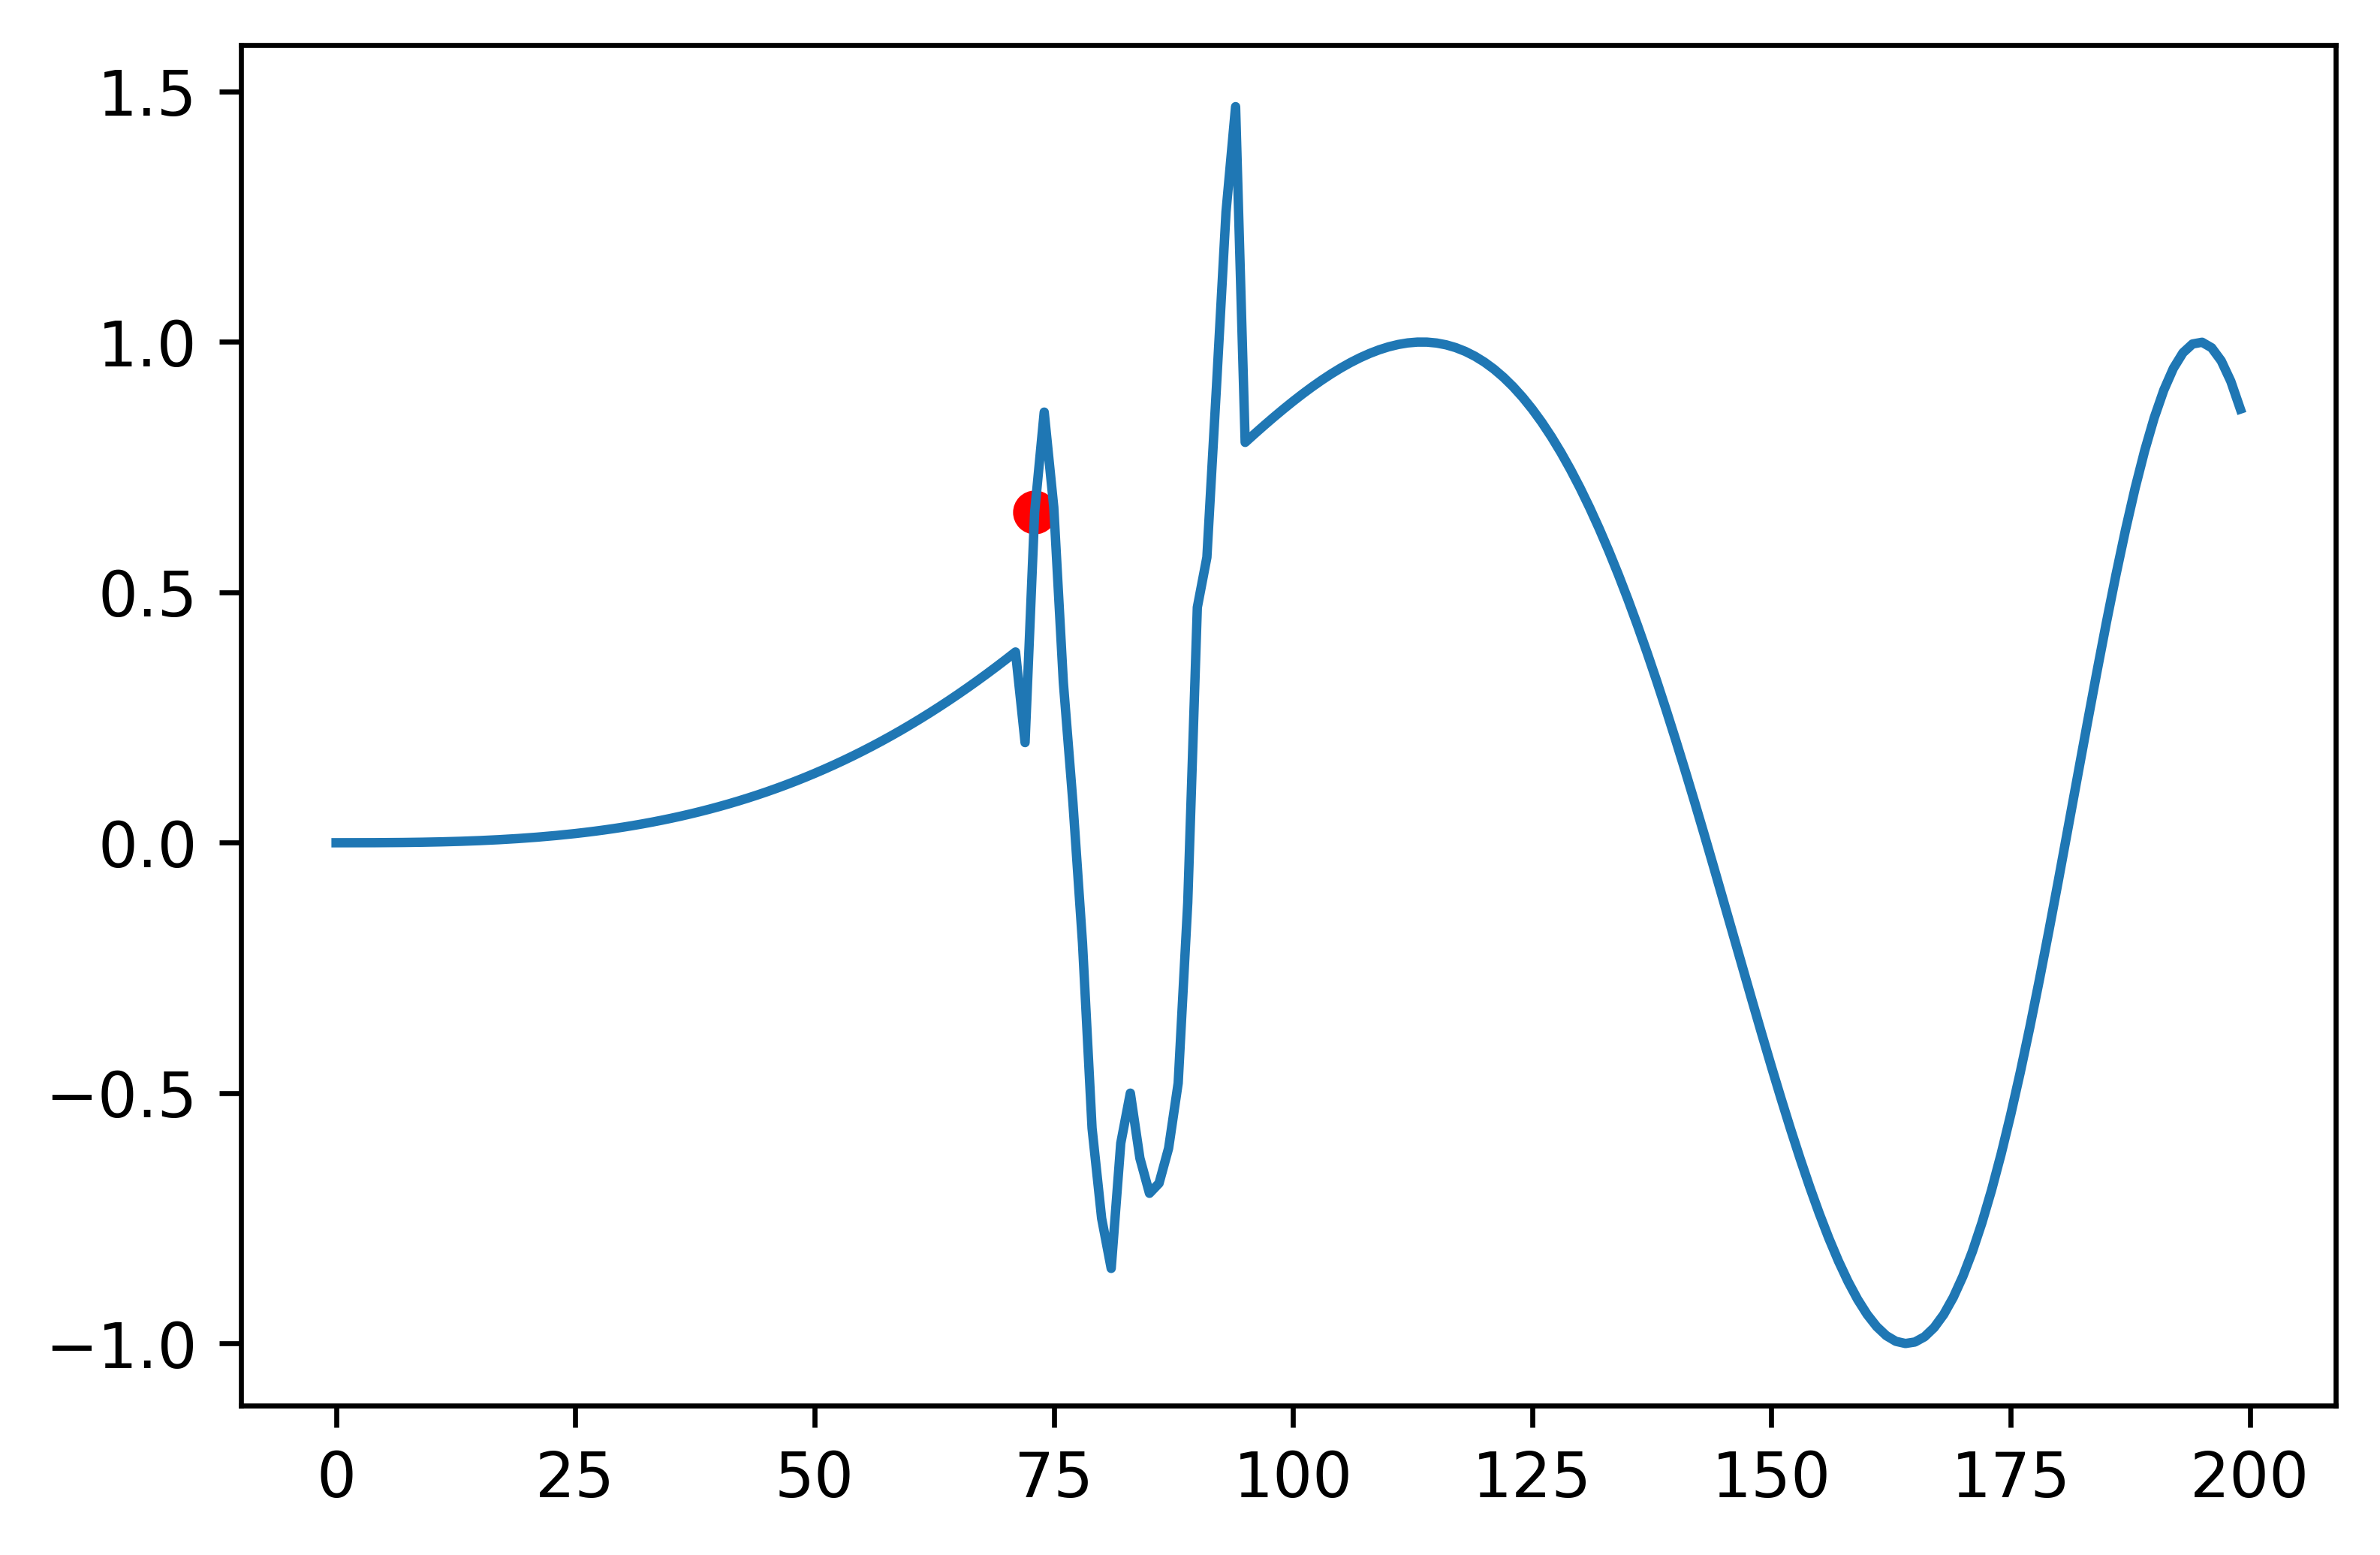
\includegraphics[scale=0.5]{Graphics/failed-example-signal.png}}
	\subfigure[Major shapelet]{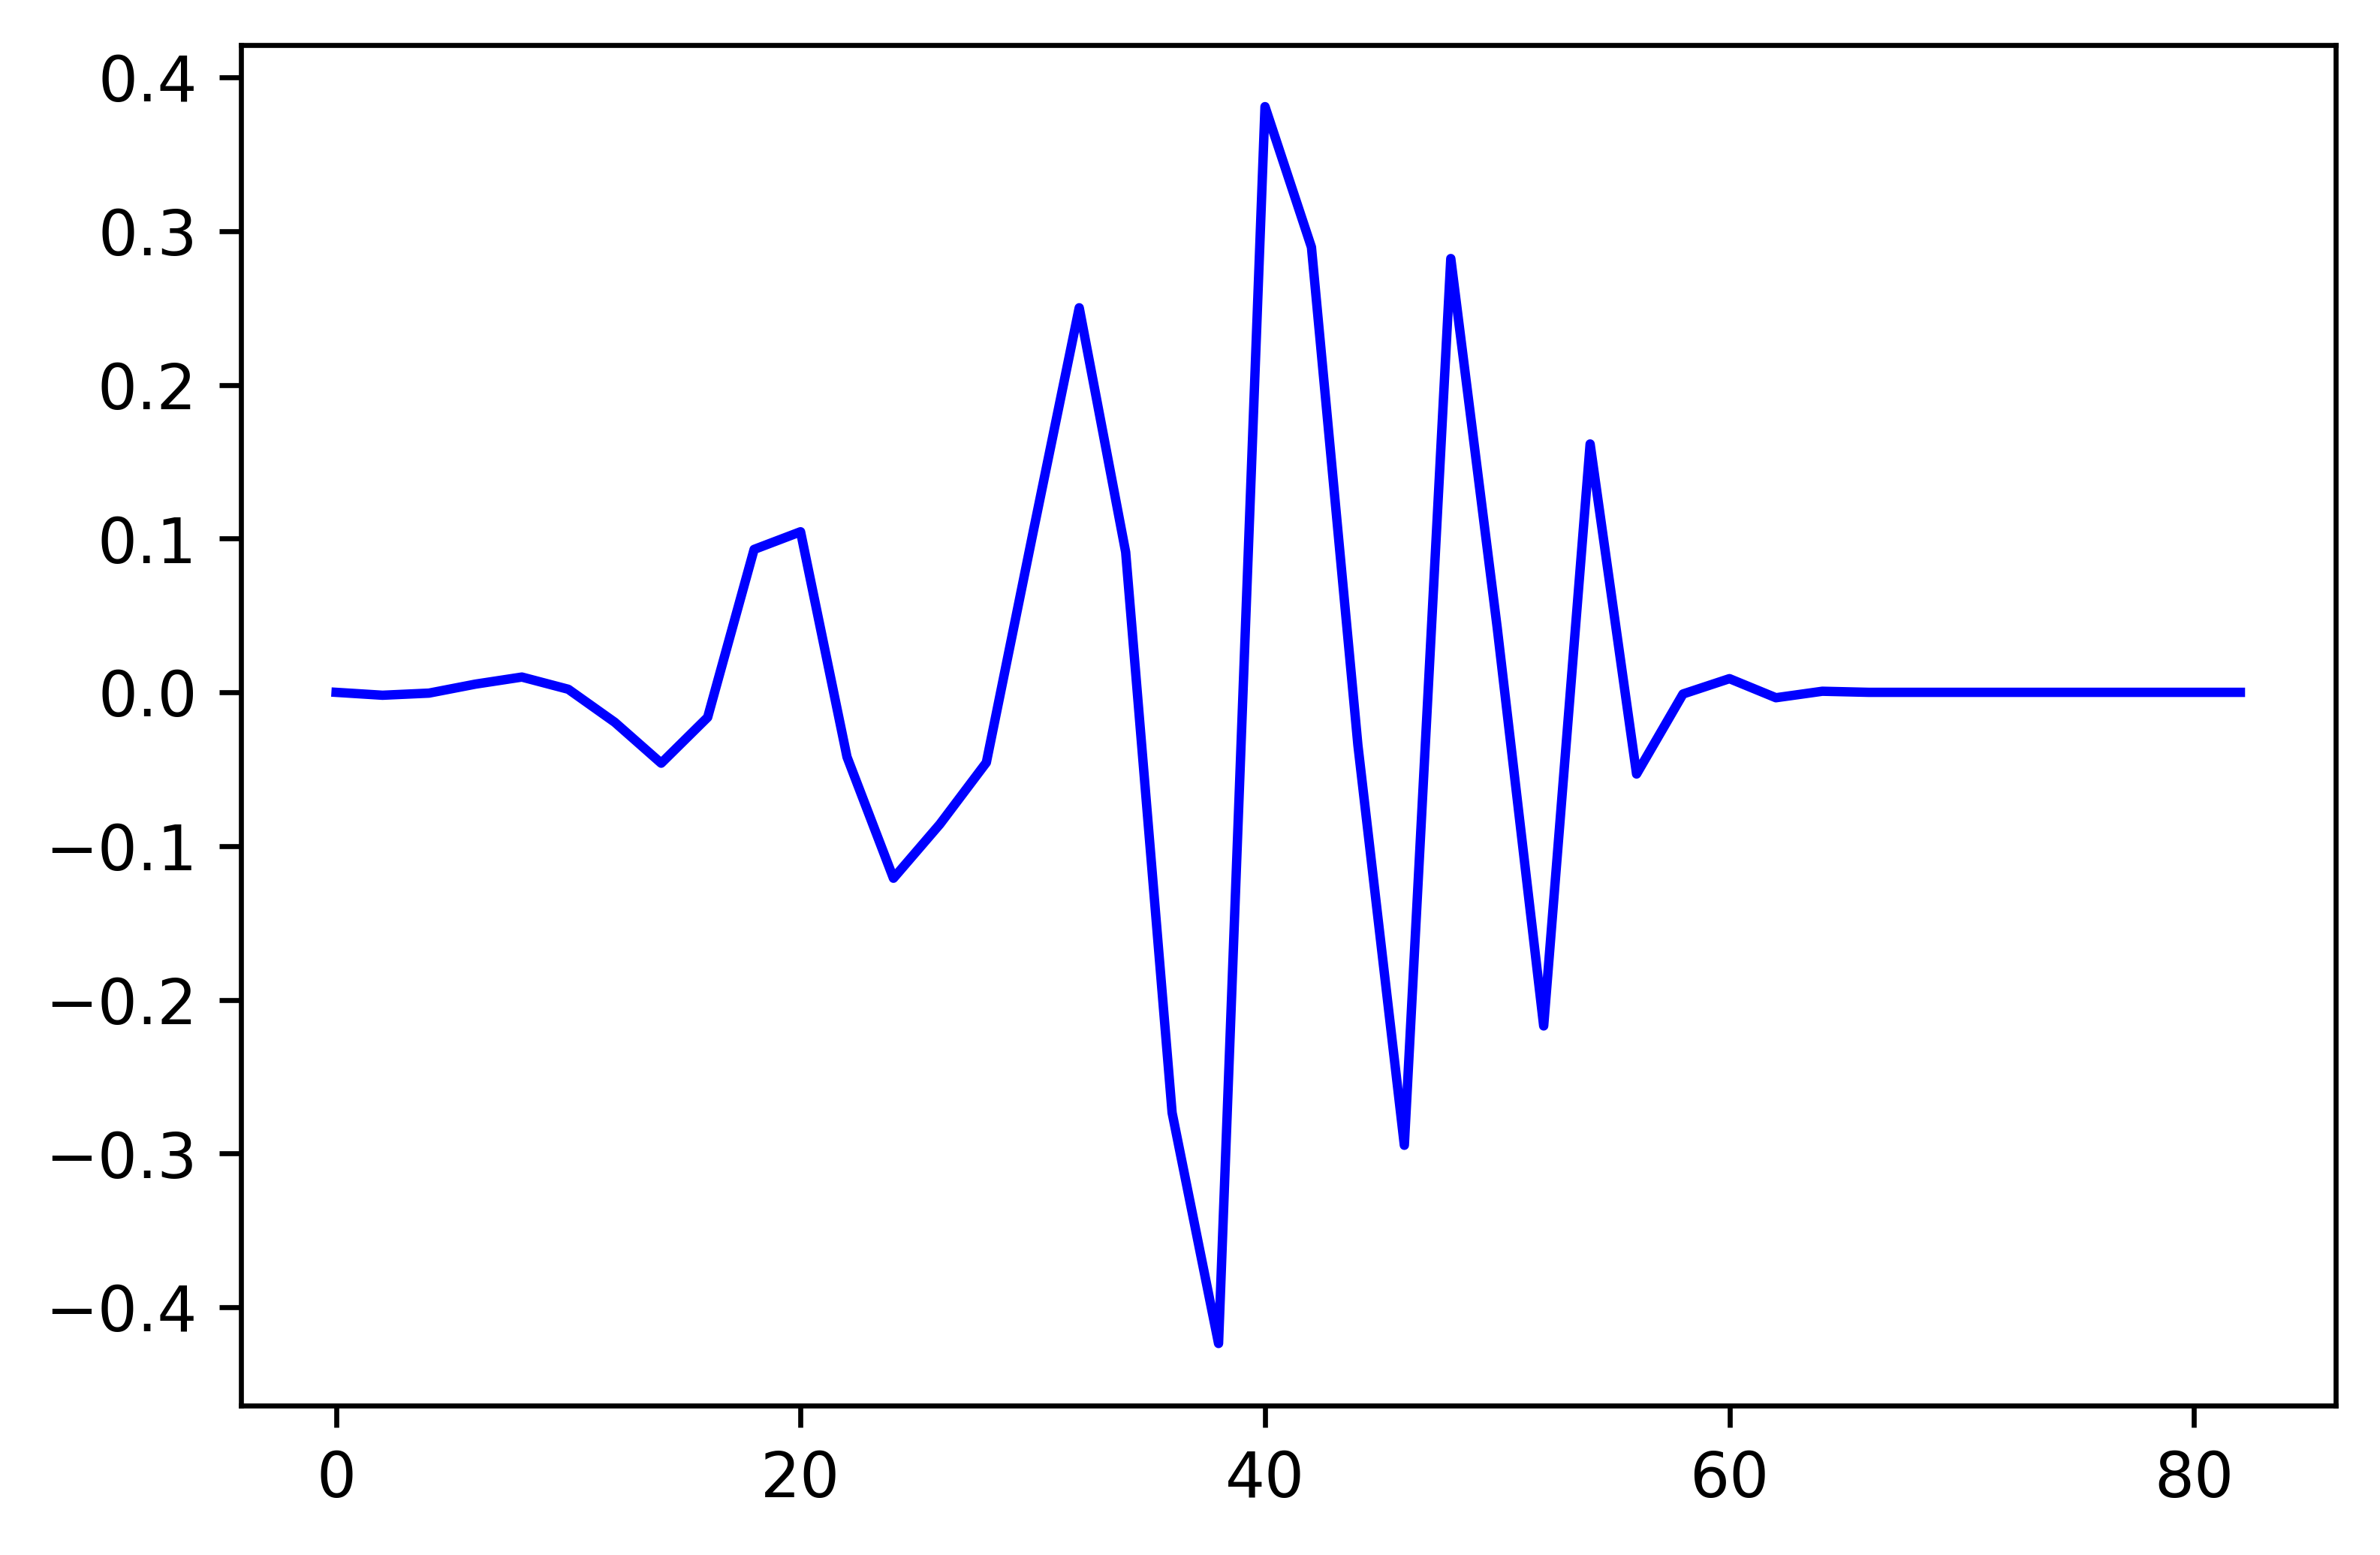
\includegraphics[scale=0.5]{Graphics/failed-example-blue-shapelet.png}}
	\subfigure[Minor shapelet]{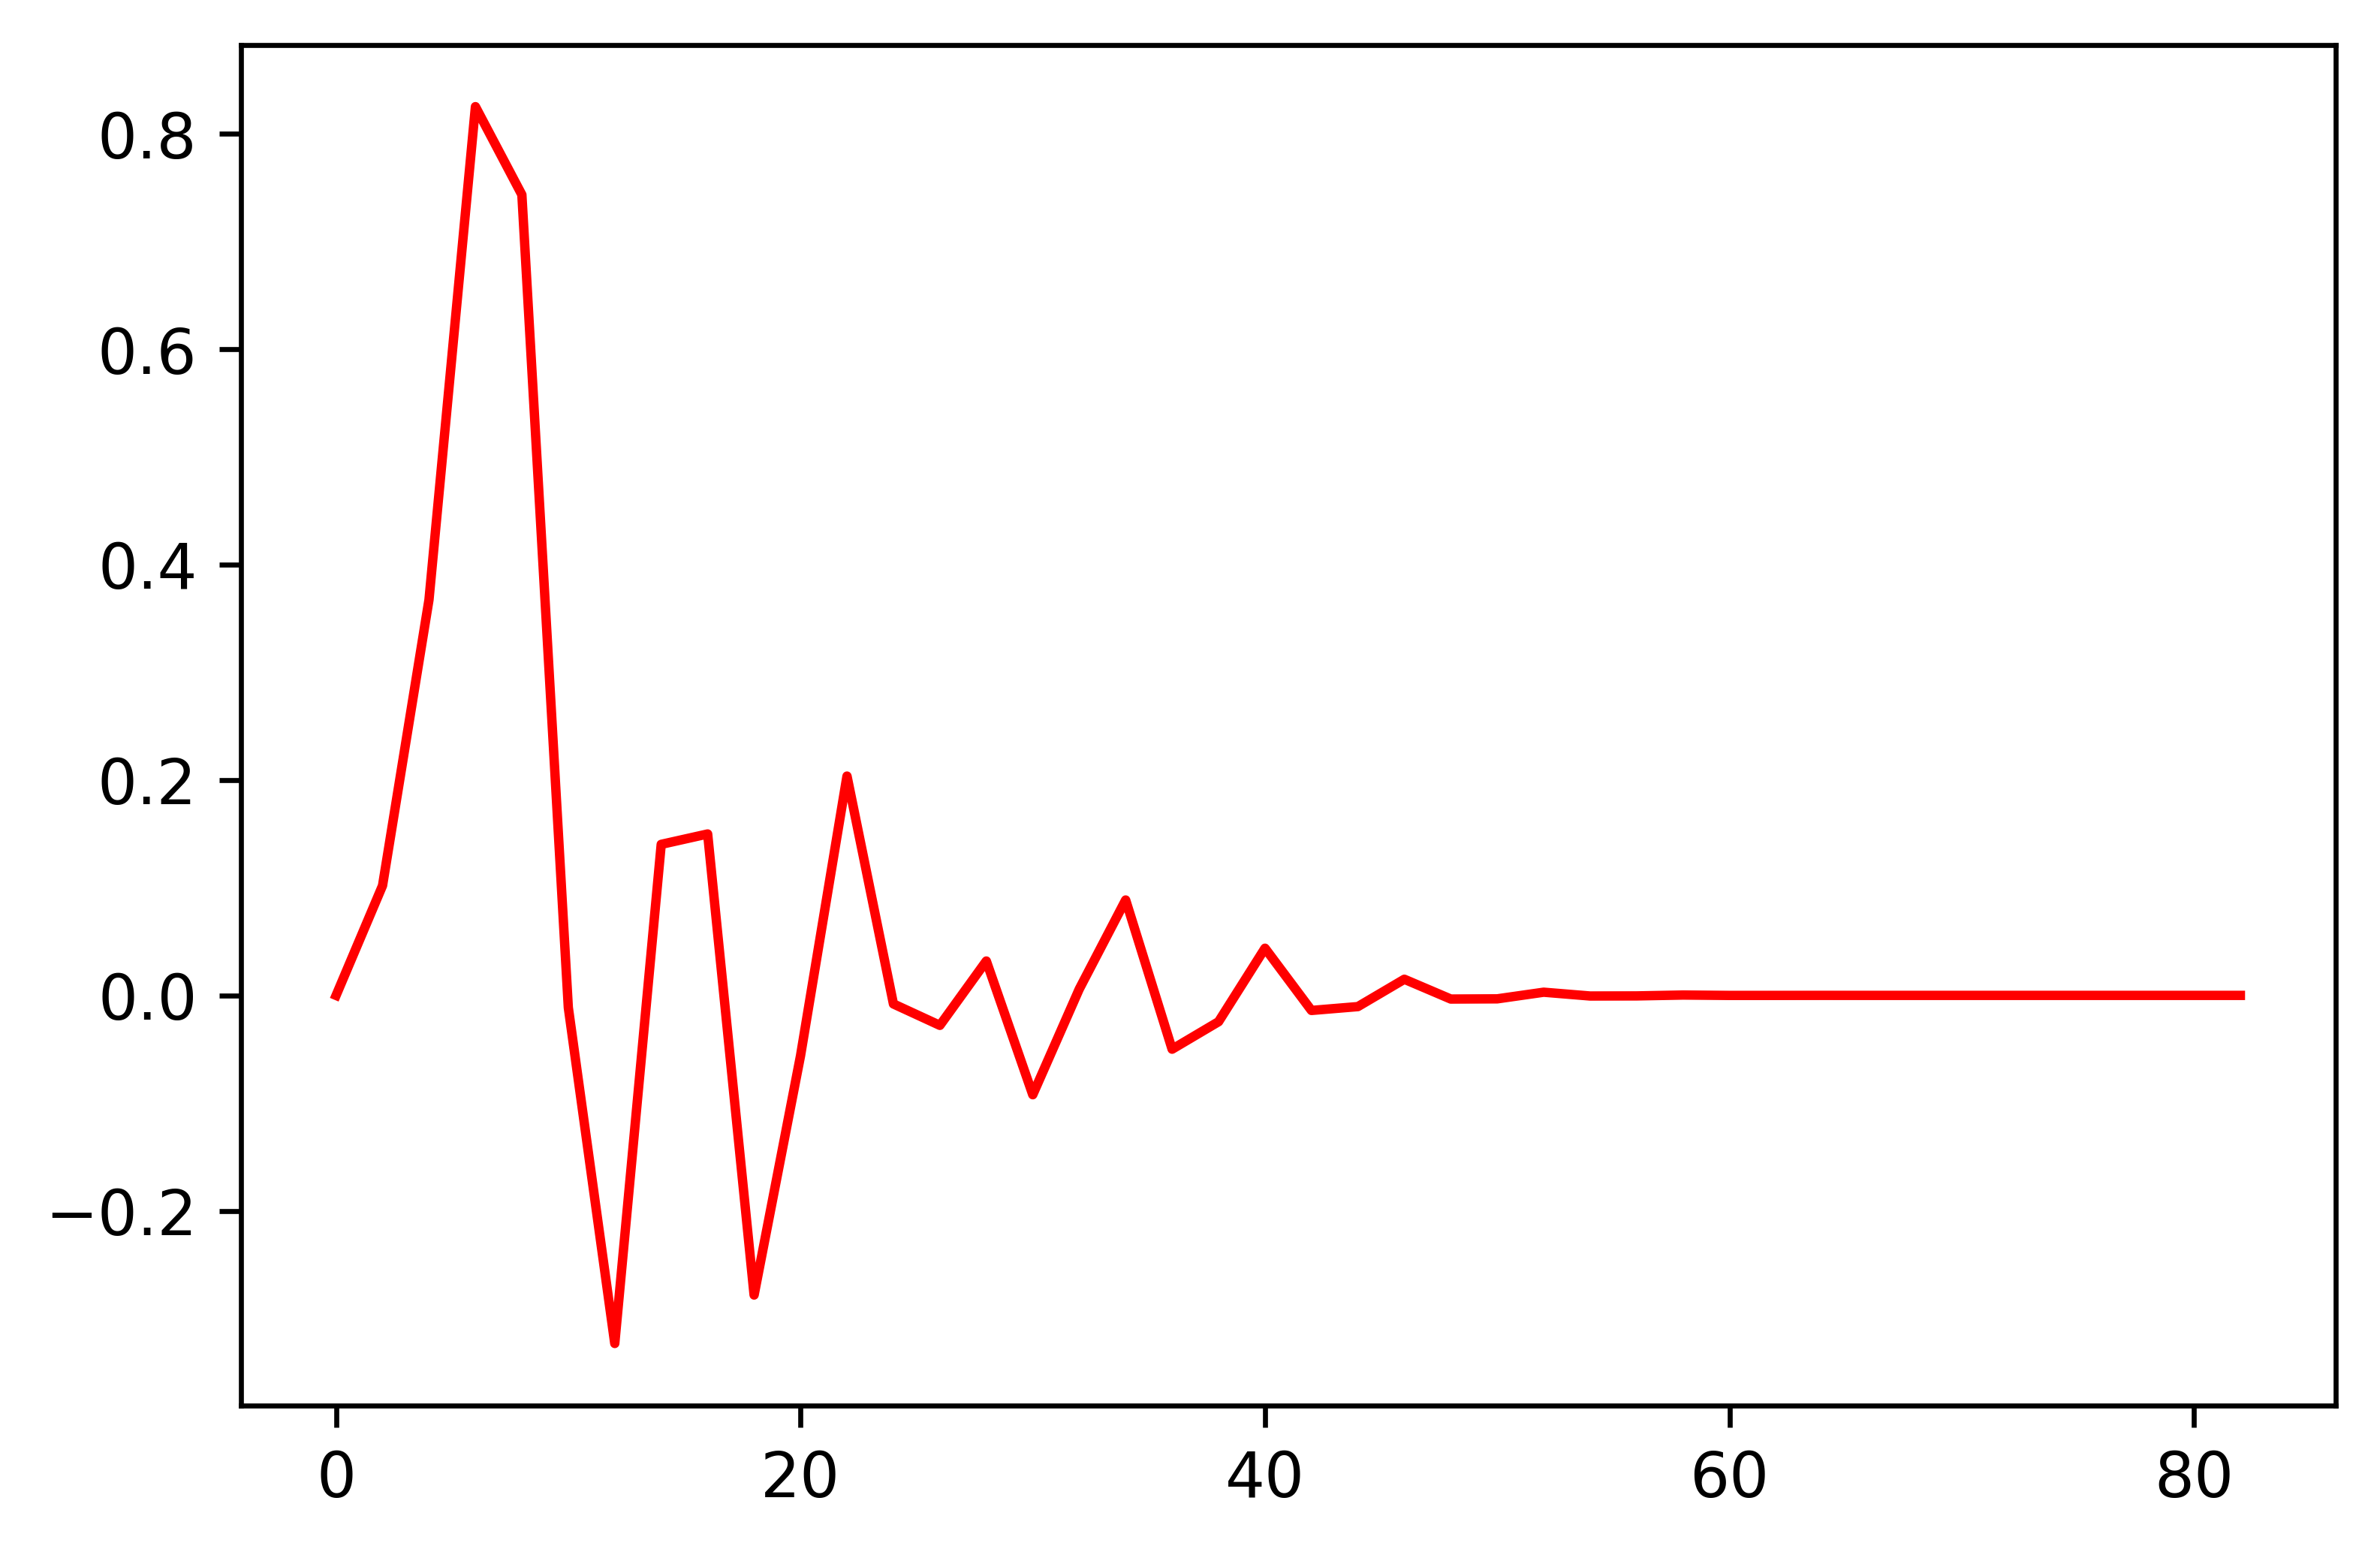
\includegraphics[scale=0.5]{Graphics/failed-example-red-shapelet.png}}
	\subfigure[DST-II y medida $\mathbb{S}$]{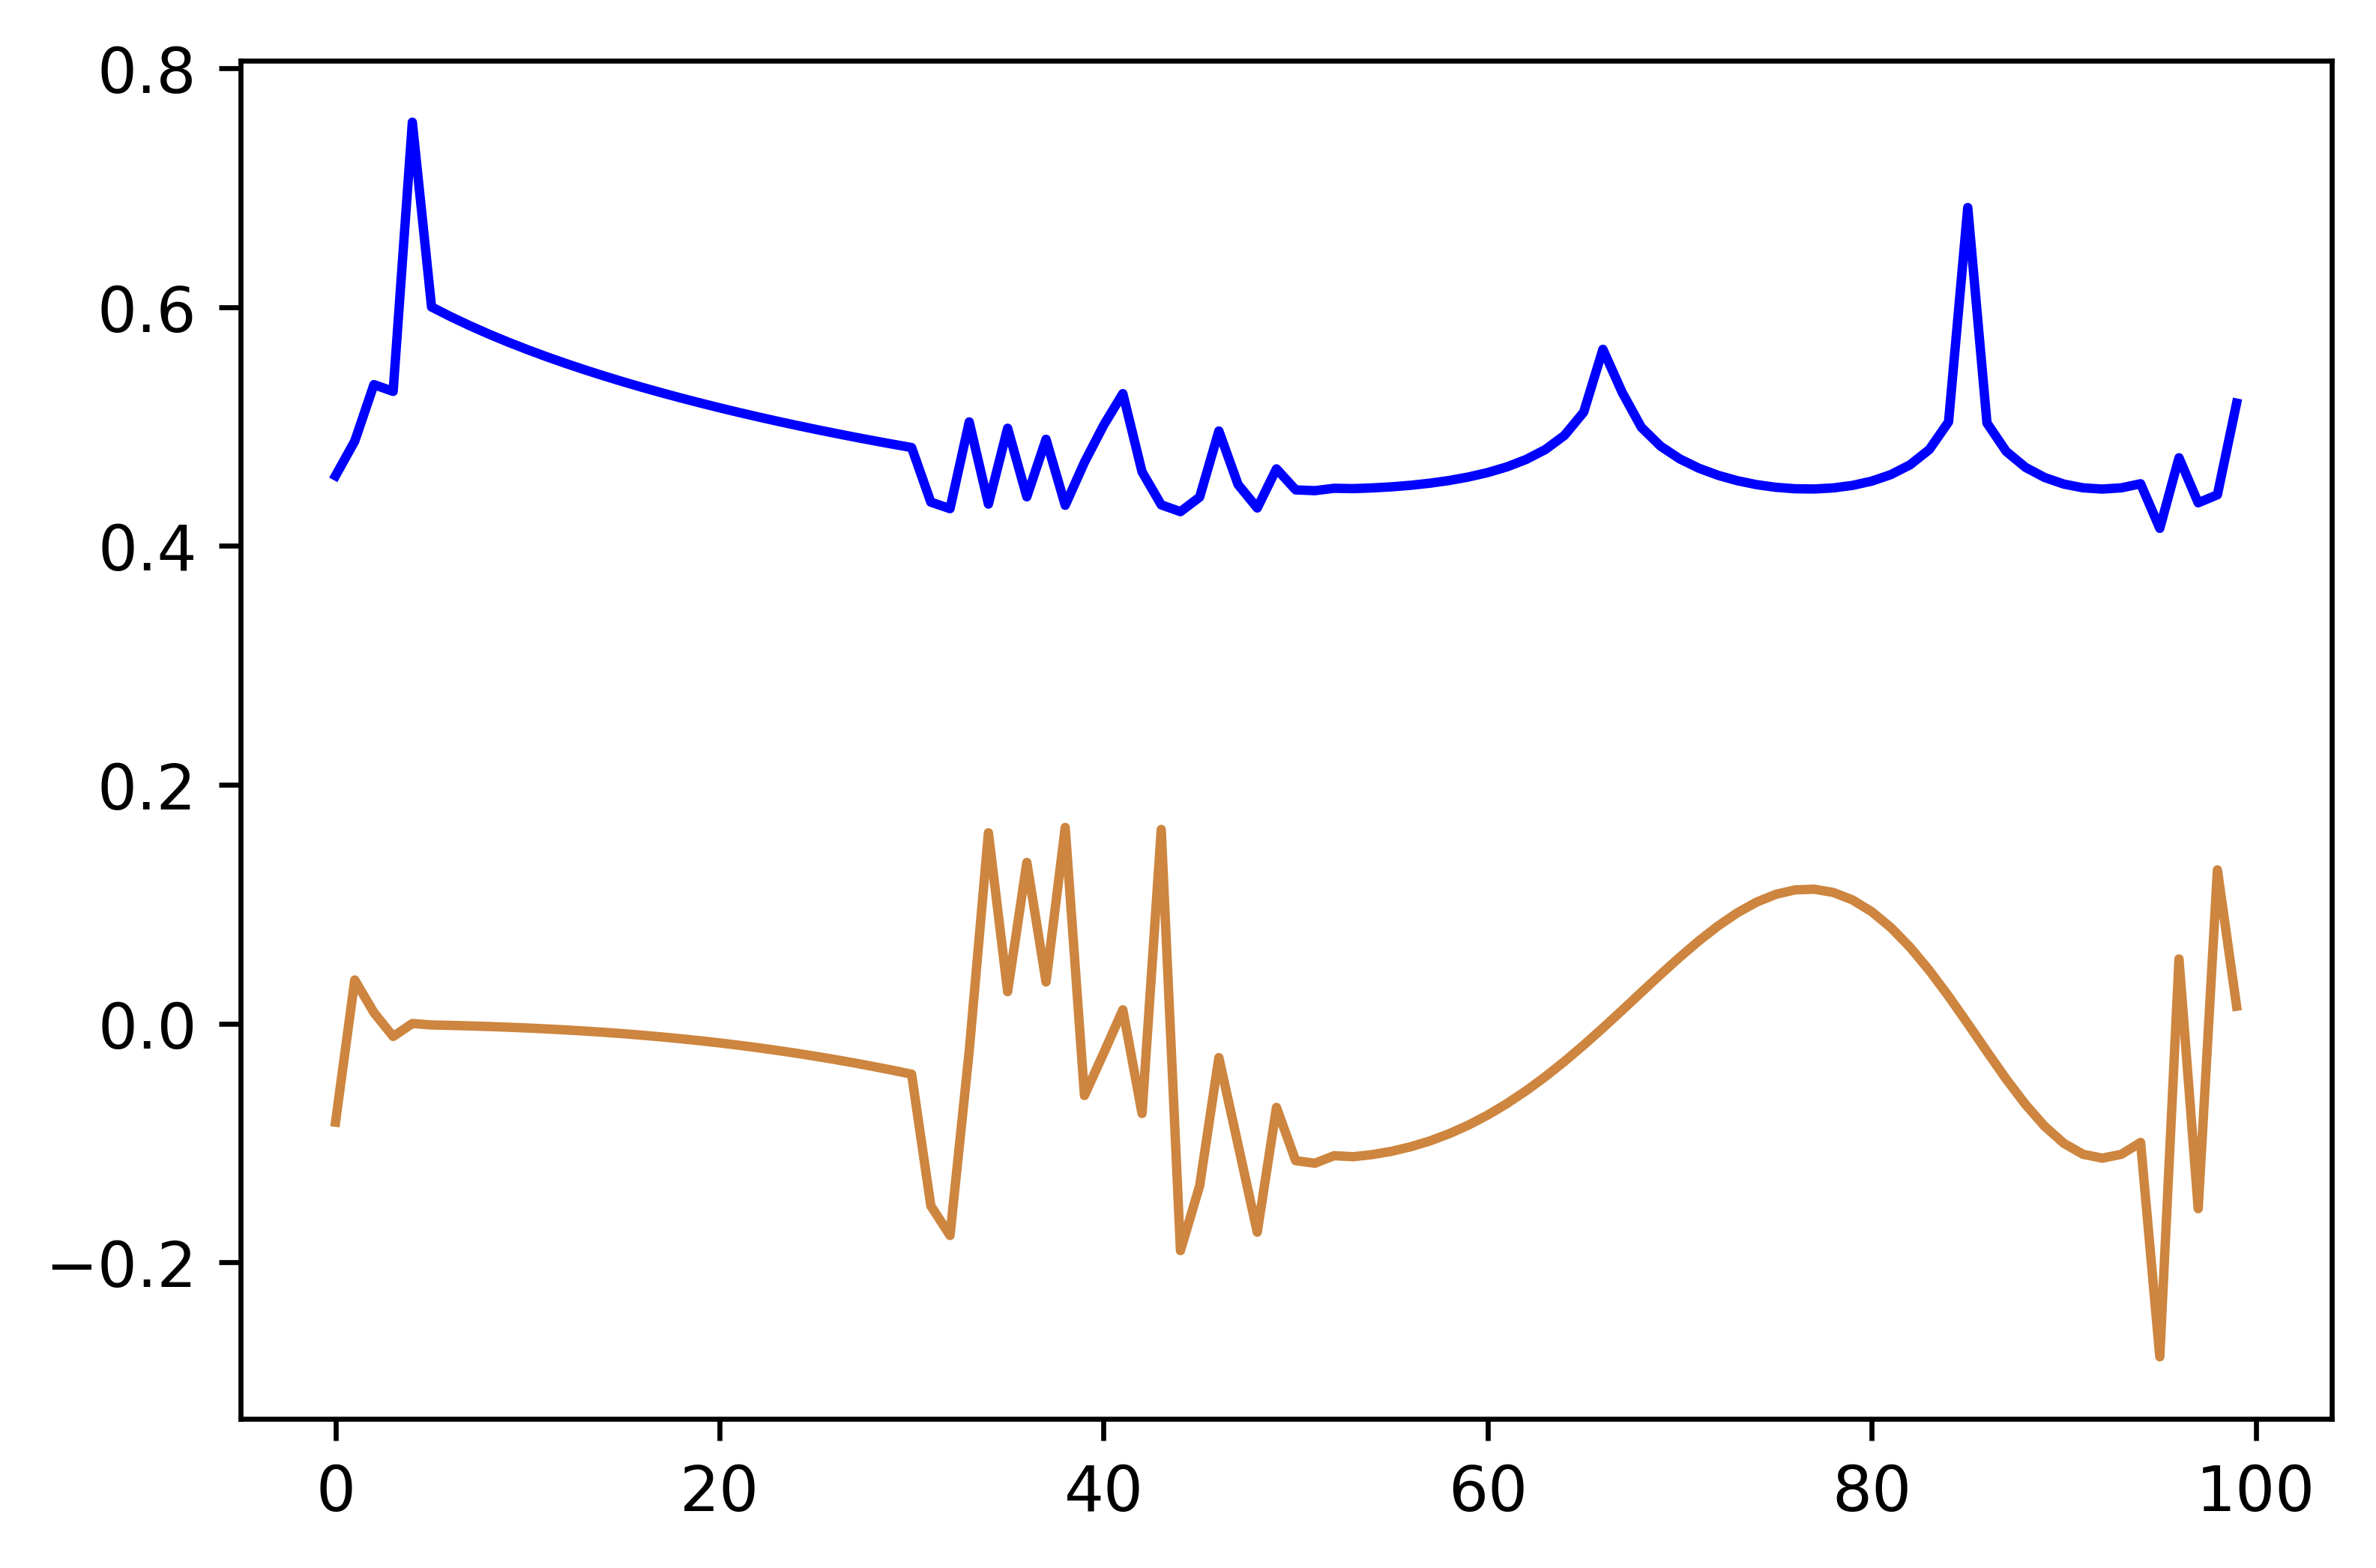
\includegraphics[scale=0.5]{Graphics/failed-example-detection.png}}
	\caption{Ejemplo donde el algoritmo no logra detectar la posición donde se encuentra el patrón.} \label{fig:failed-example-experiment}
\end{figure}

\section{Detección de patrones en señales 2D}

Una vez evaluada la capacidad de detección de la DST-II, se procede a la exploración de sus capacidades 
para el caso de señales 2D. A continuación se describen en detalles de los experimentos y resultados.

Para llevar a cabo la experimentación se crearon imágenes artificiales con figuras simples. Entre ellas se incluyen gaussianas,
círculos y zonas rectangulares. El objetivo es evaluar la capacidad del algoritmo para detectar en el caso de 2D
y su sensibilidad ante el ruido. Sobre cada una de estas figuras se utilizó cada una de las propuestas realizadas 
en la Sección \ref{section:2d}.
El resultado se evaluaba visualmente, sobre el  mapa de colores (Figura \ref{fig:colormap}) donde las tonalidades azules representas
valores cercanos a 0 y las amarillas cercanas a 1.

\begin{figure}
	\centering
	
\includegraphics[scale=0.8]{Graphics/colormap.png} 
	\caption{Mapa de colores usado para evaluar la detección de la DST-II. Valores pequeños son representados en tonalidades azules y valores altos en amarillo.} \label{fig:colormap}
\end{figure}

\subsection{Ejemplos de los experimentos y análisis de los resultados}

\begin{figure}
	\centering
	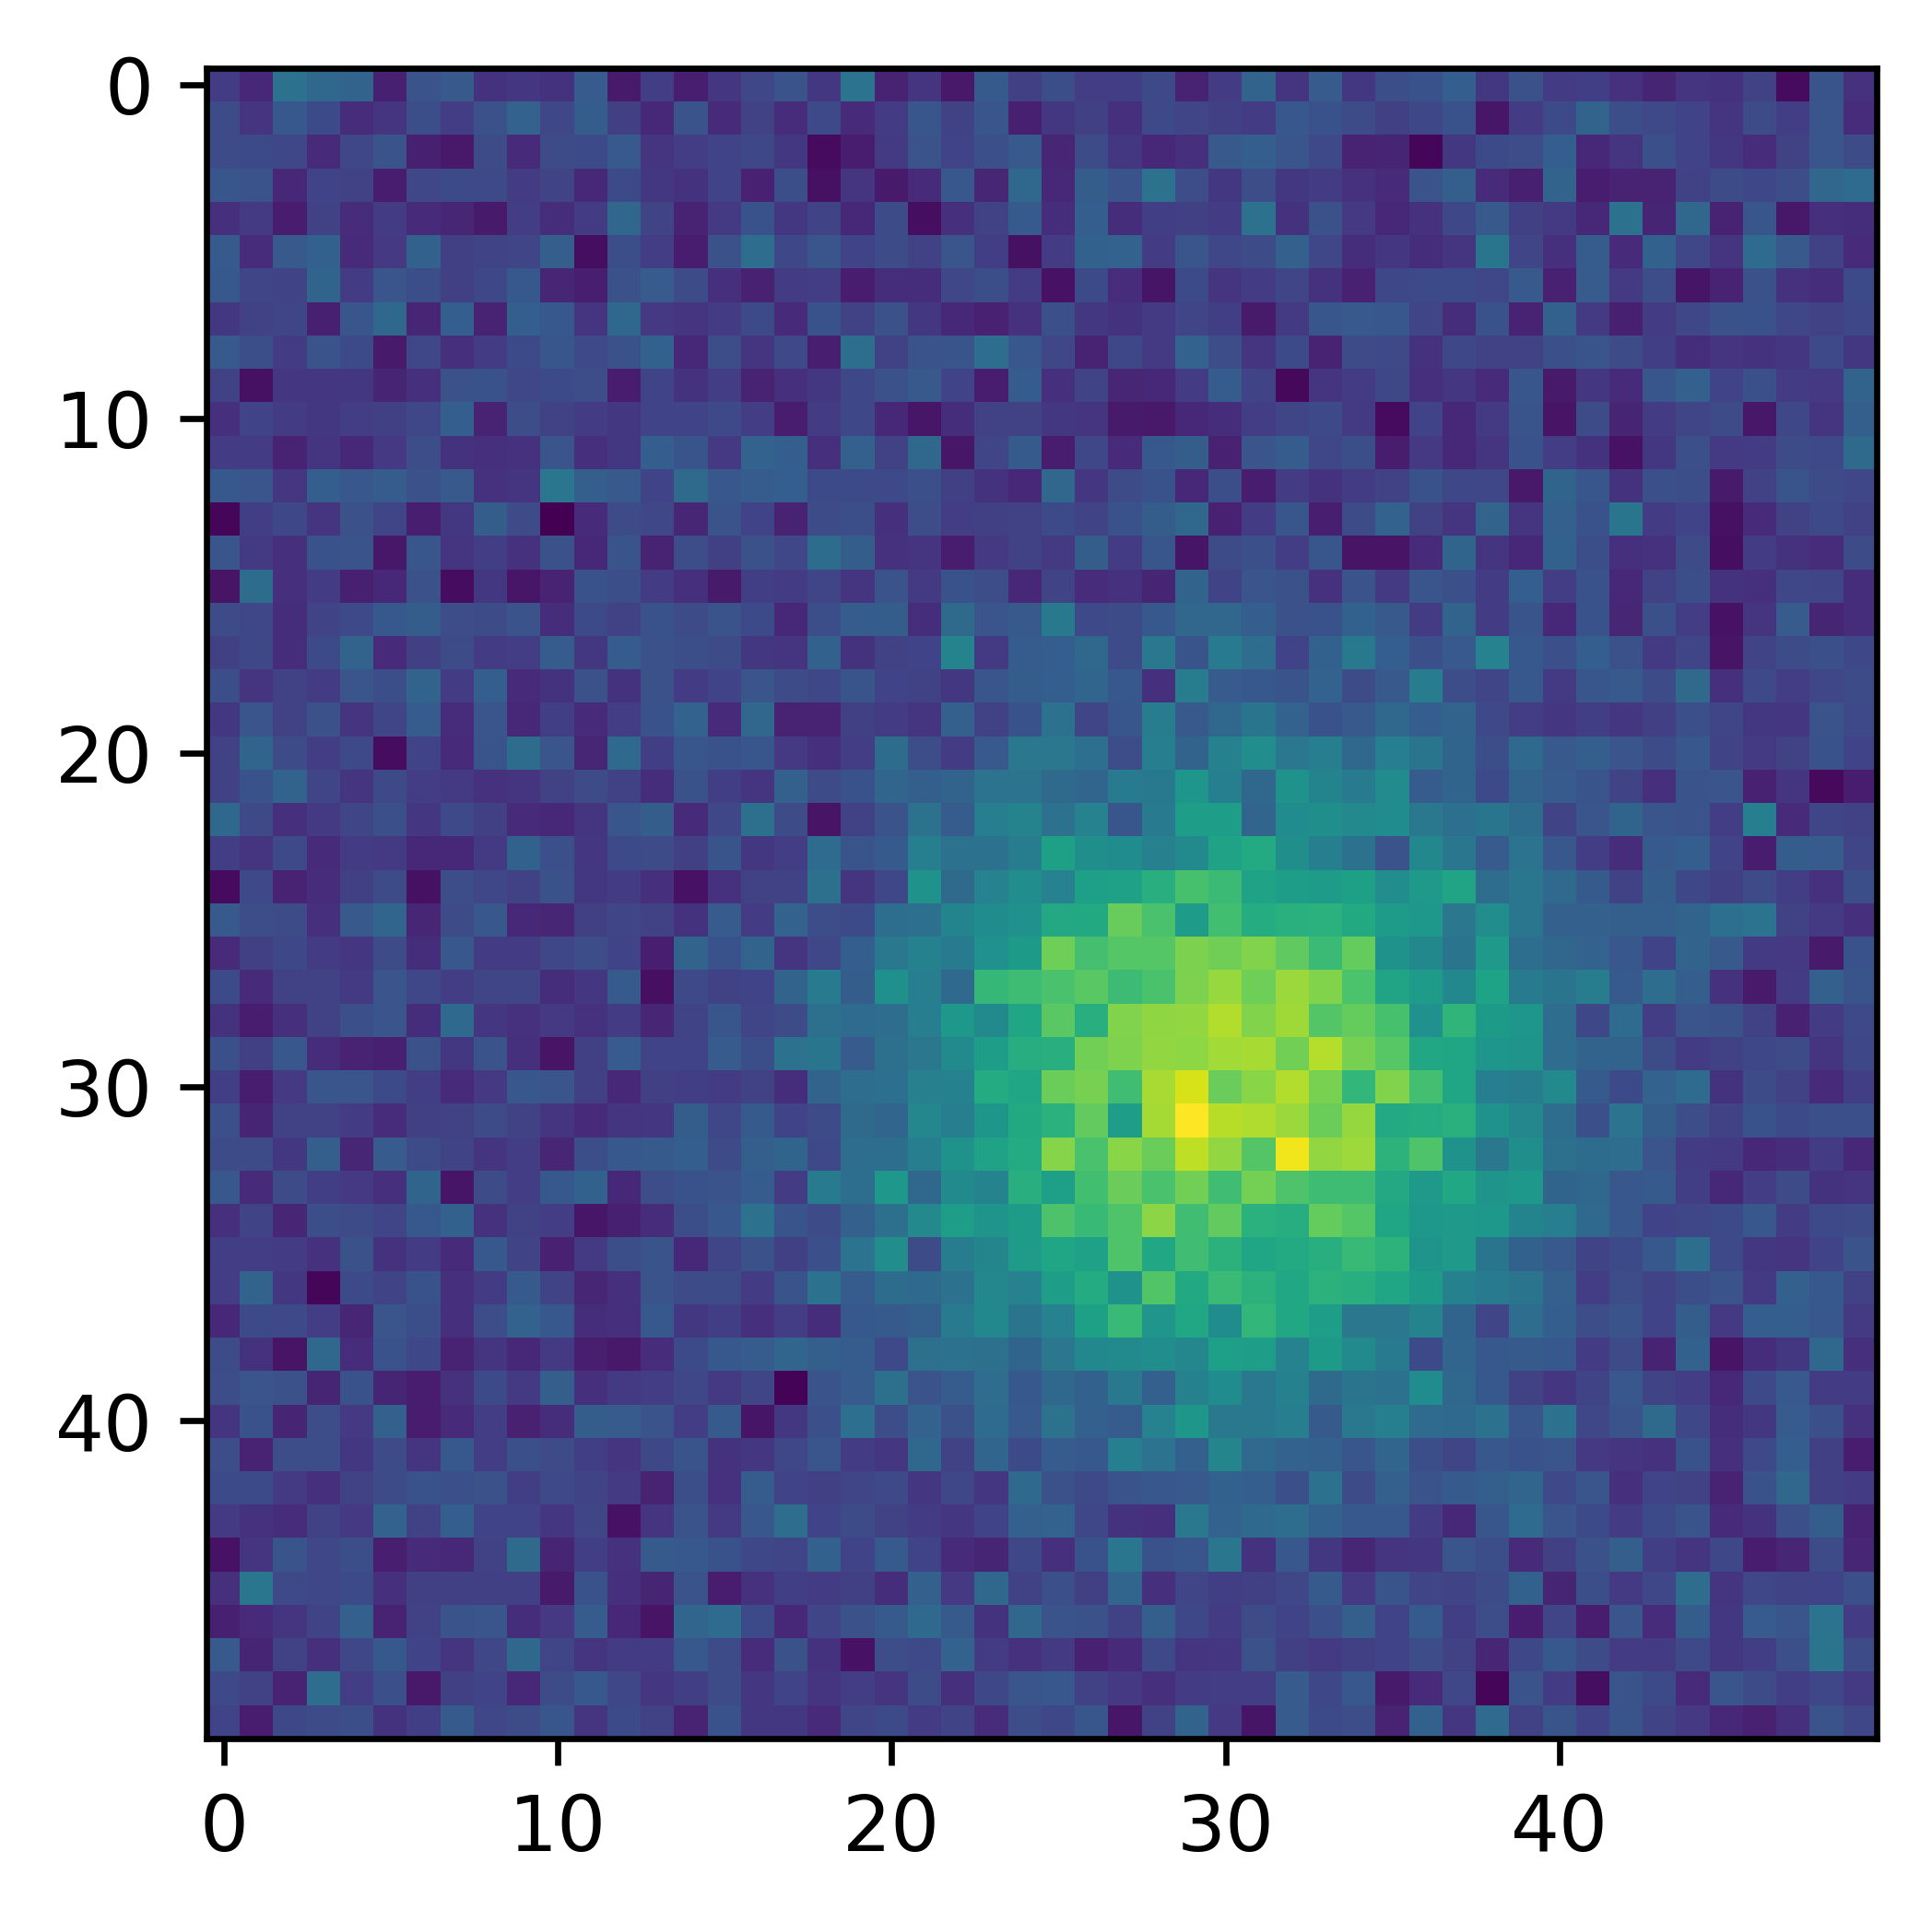
\includegraphics{Graphics/gaussian-2d-experiment.png}
	\caption{Gaussiana centrada en la posición (30,30).} \label{fig:gaussian-example-experiment}
\end{figure}

\begin{figure}
	\centering
	\subfigure[Sección horizontal]{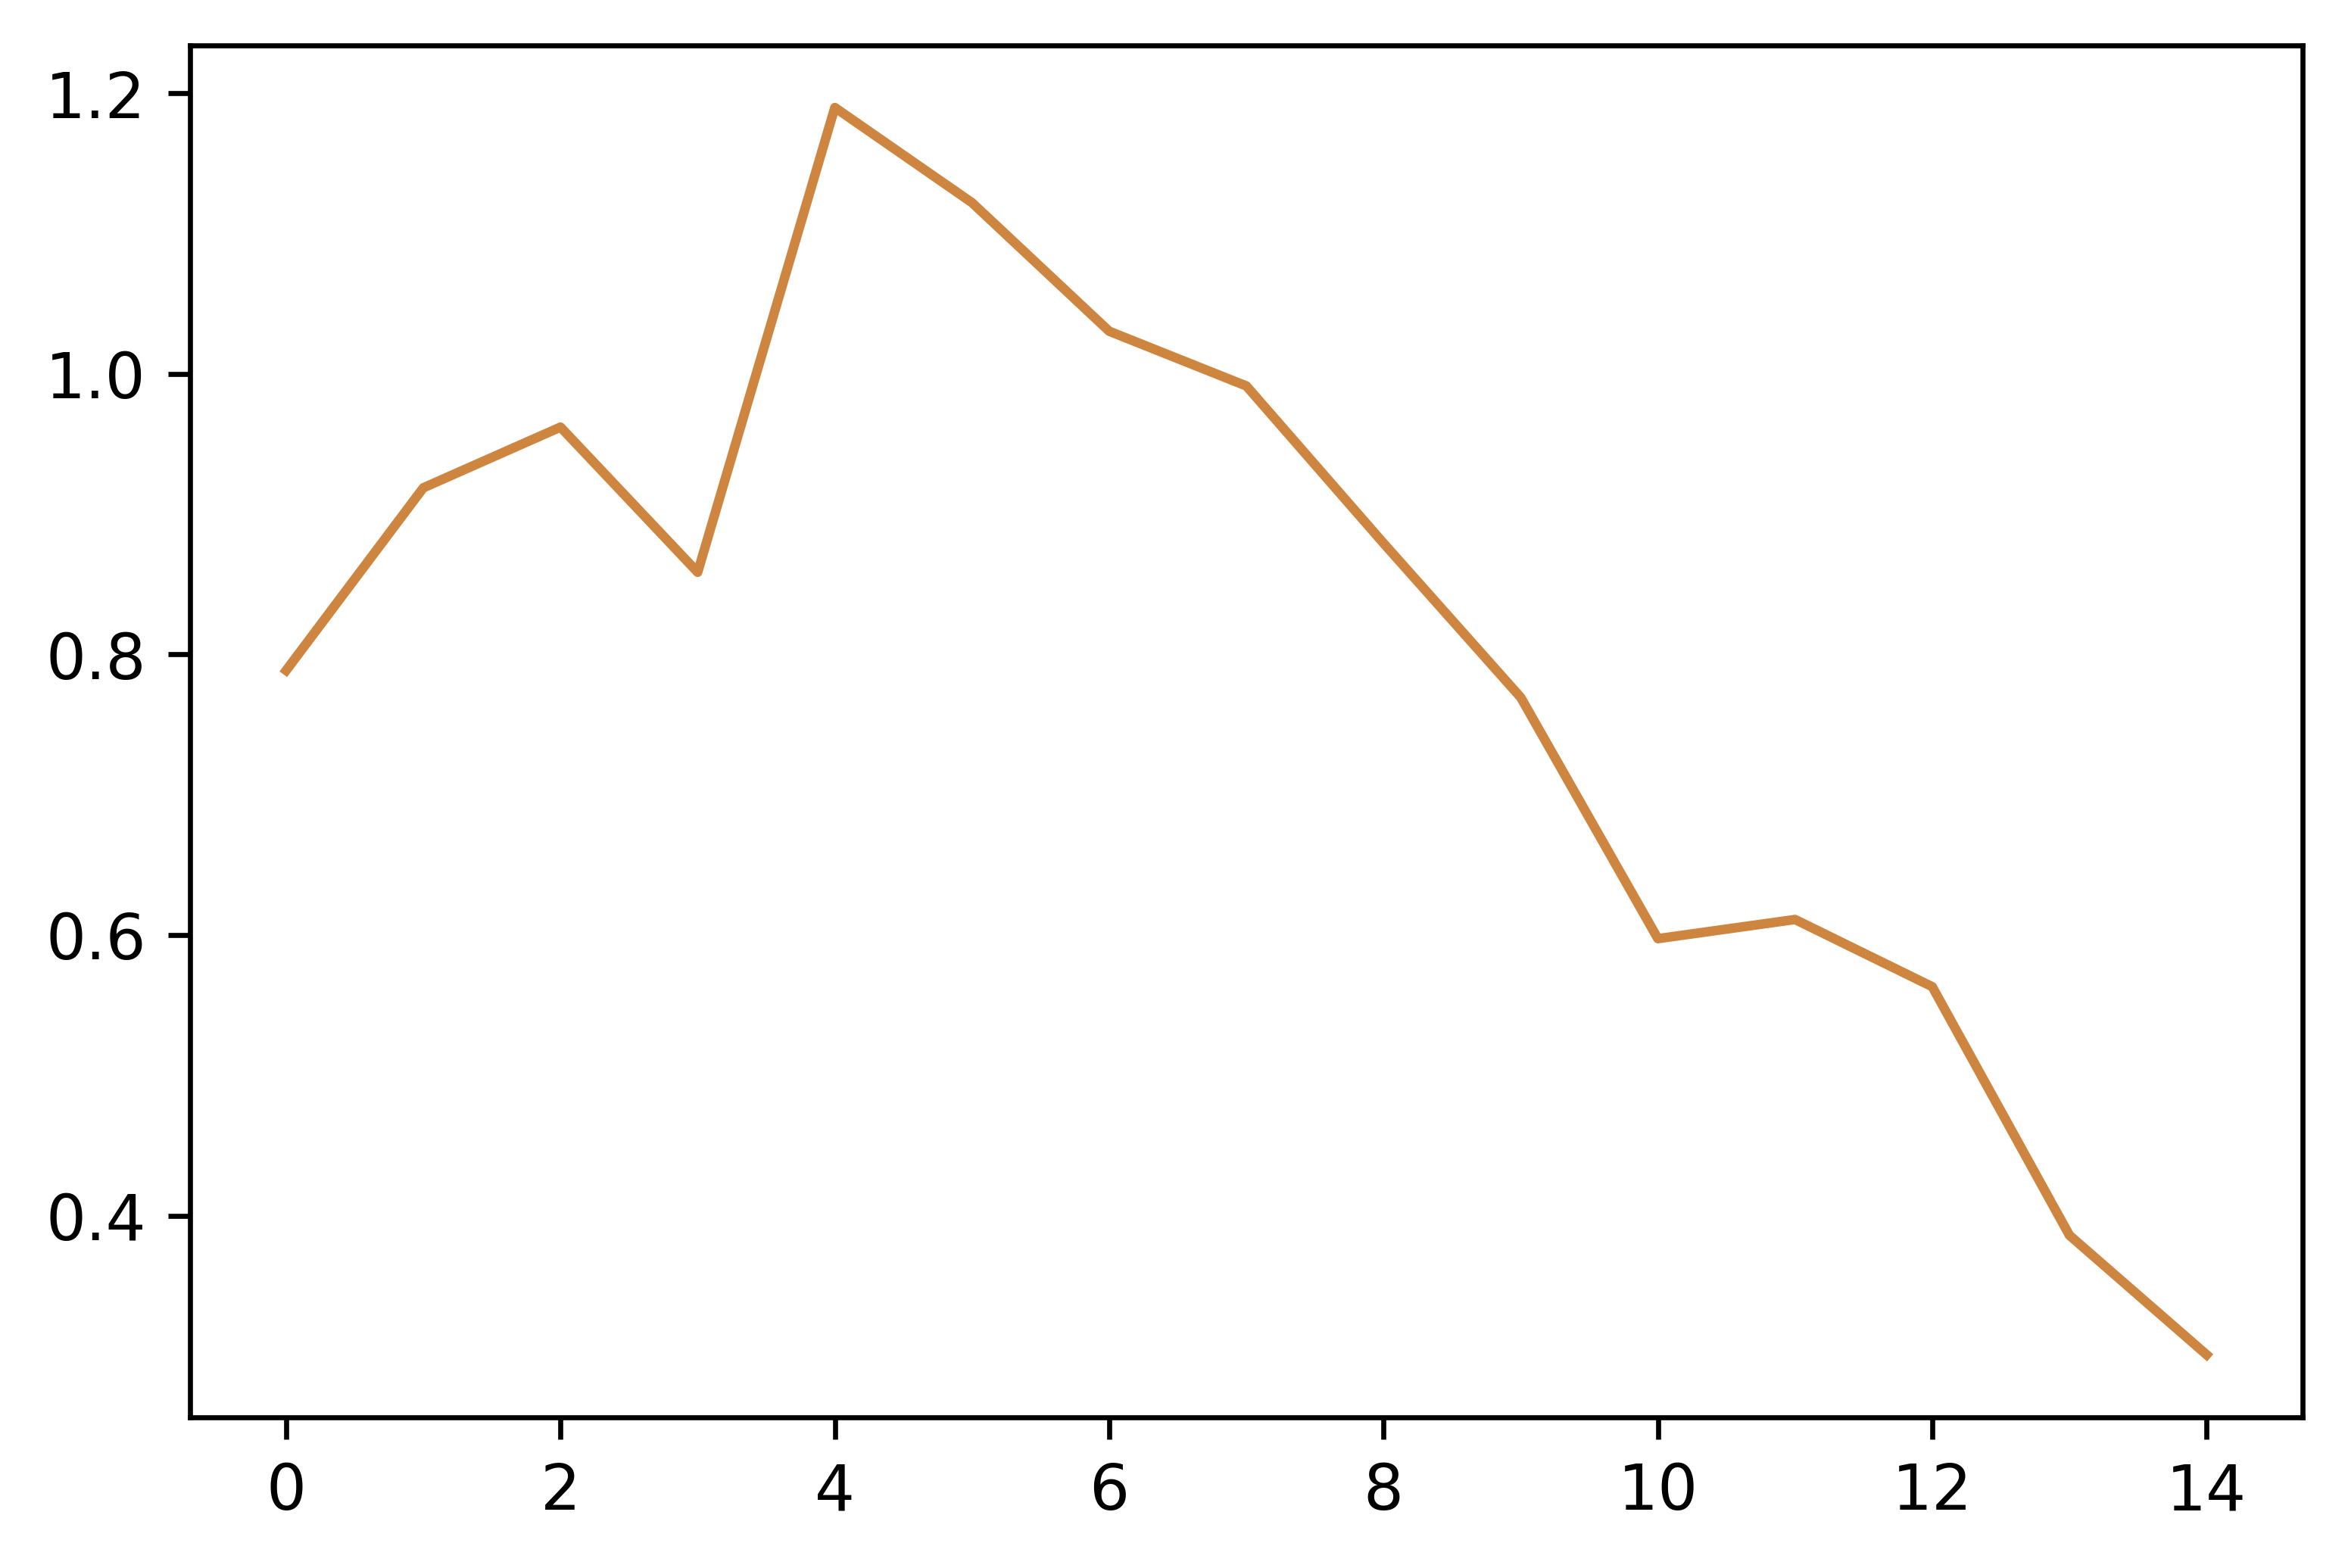
\includegraphics[scale=0.5]{Graphics/line-gaussian-experiment.png}}
	\subfigure[Sección vertical]{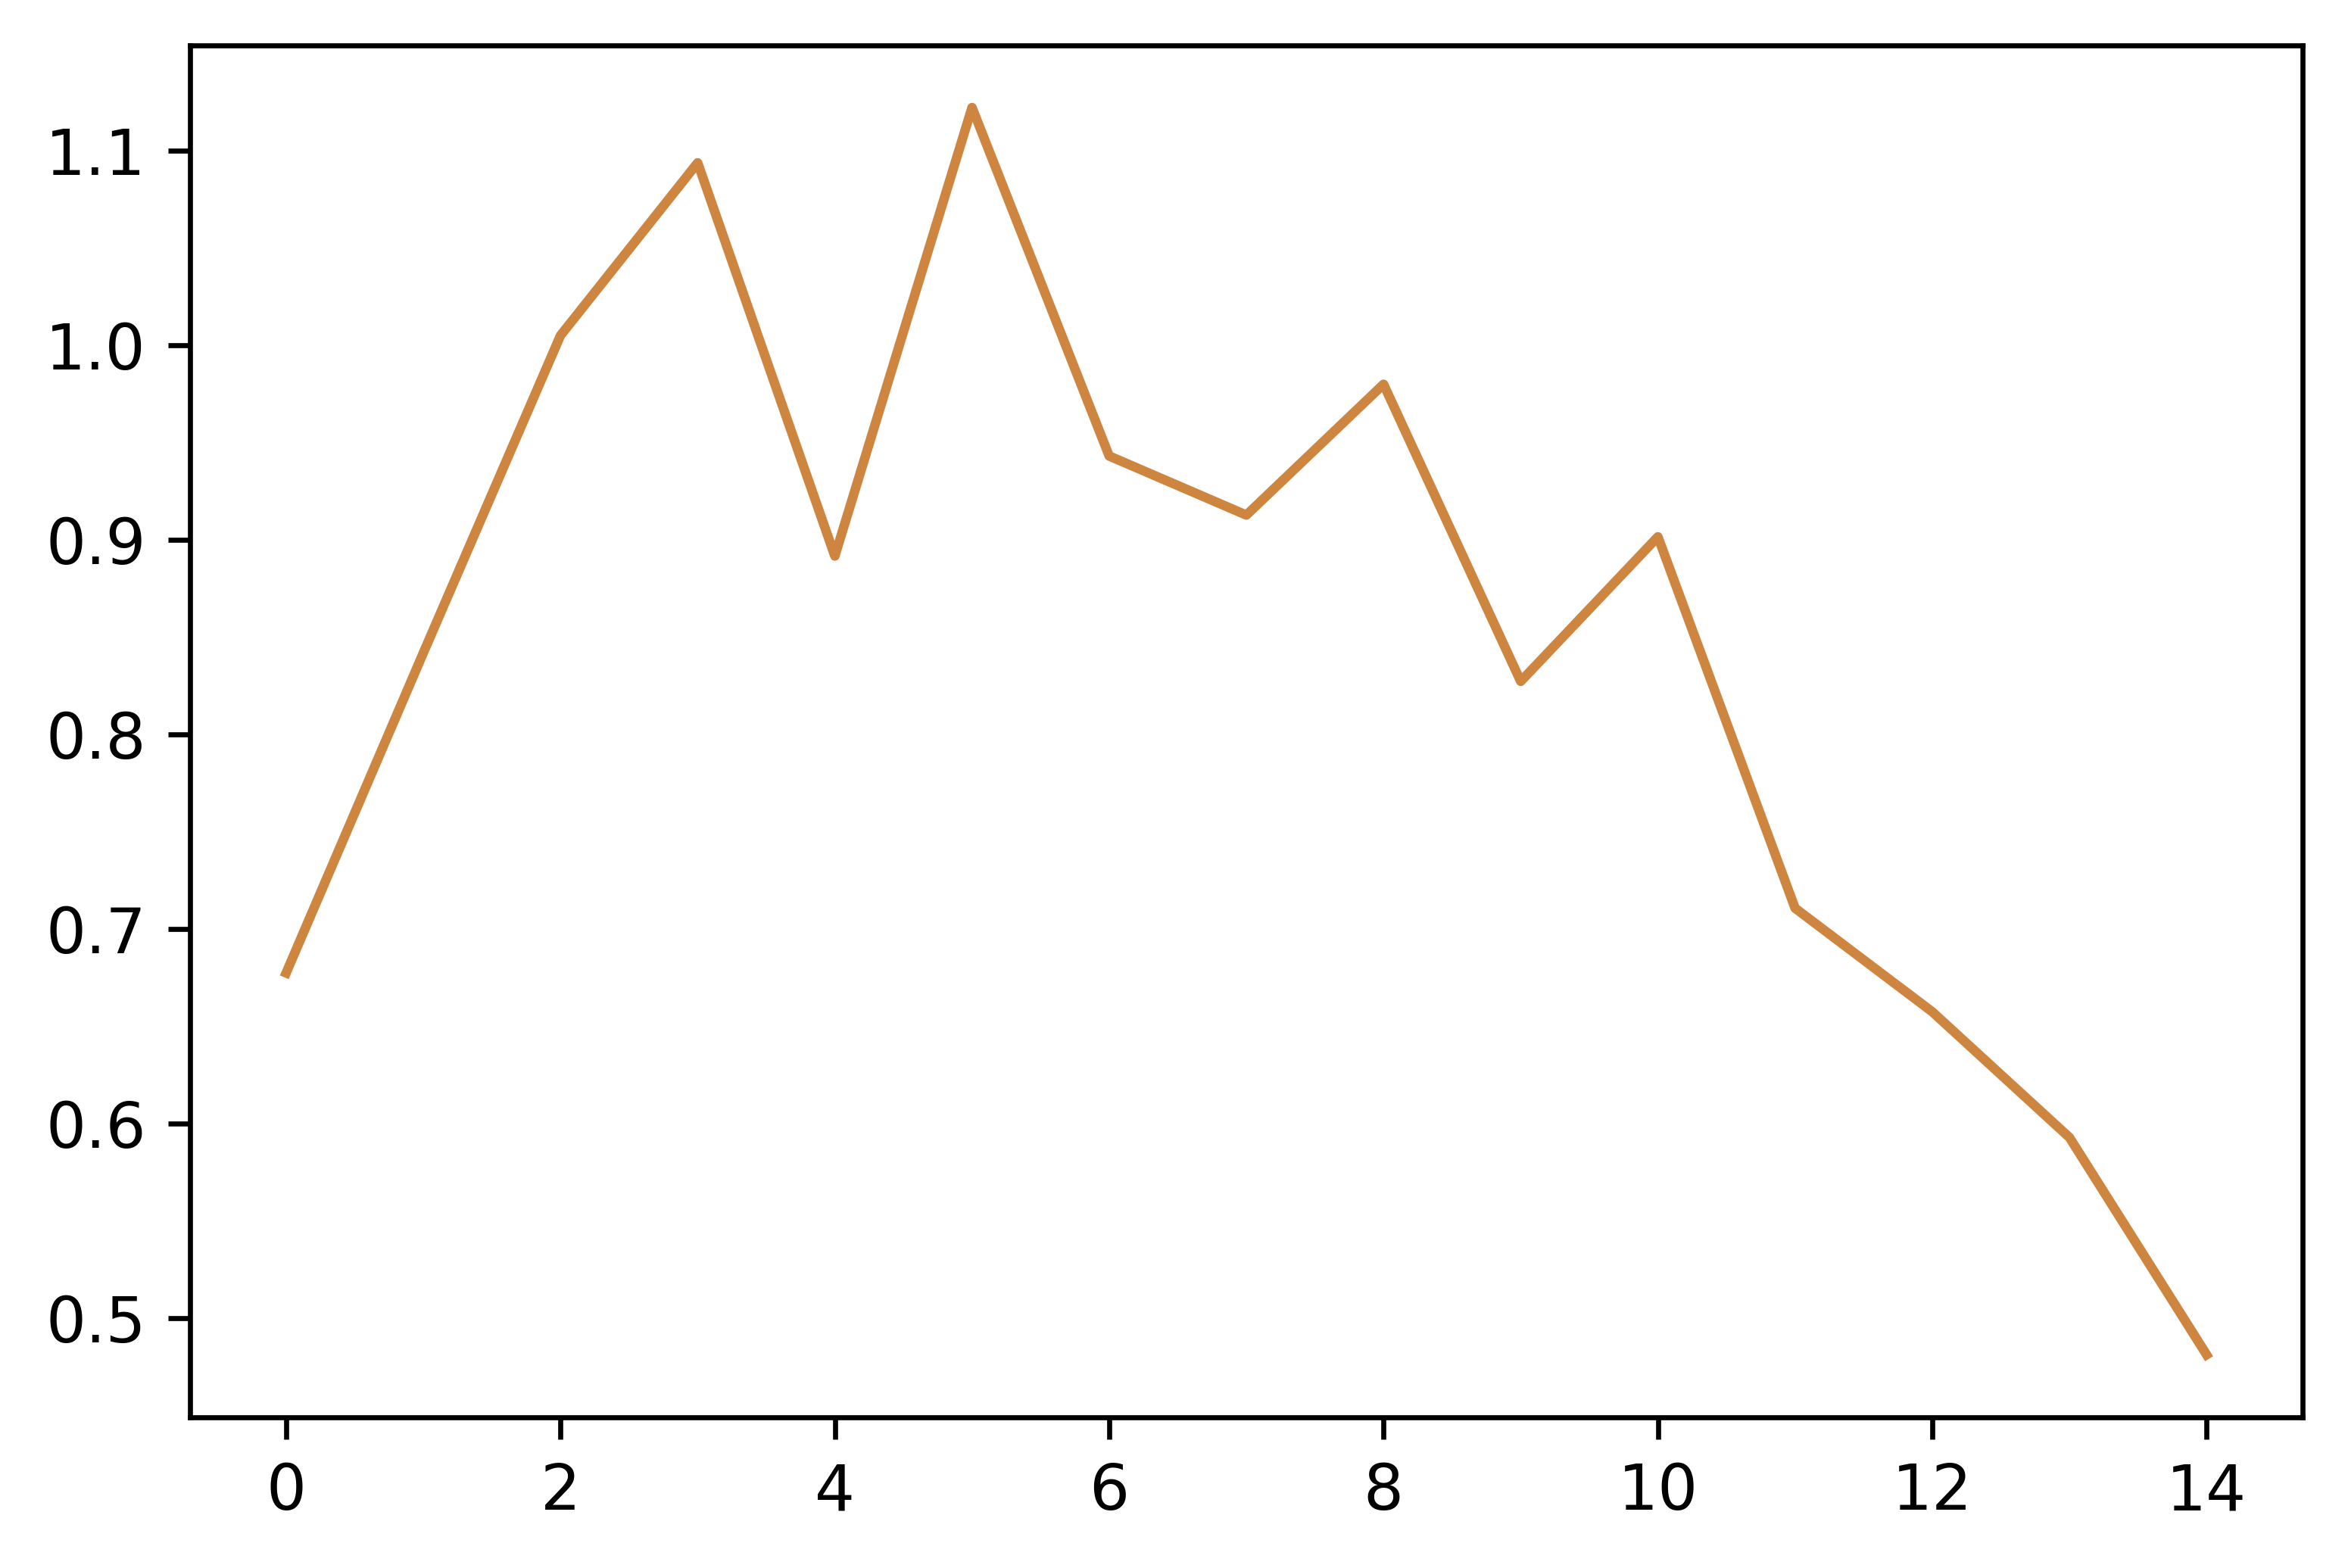
\includegraphics[scale=0.5]{Graphics/line-gaussian-experiment-vertical.png}}
	\caption{ Secciones correspondientes a [30,25:40] y [25:40,30] de la Figura \ref{fig:gaussian-example-experiment}.} \label{fig:lines-experiment}
\end{figure}

Como ejemplo se toma la imagen de la Figura \ref{fig:gaussian-example-experiment}. Siguiendo el primer enfoque,
se toman las secciones mostradas en la Figura
\ref{fig:lines-experiment} y se construyen dos \textit{shapelets} (una para las columnas y otra para las filas), obteniendose cuatro componentes
al realizar la transformada. La Figura \ref{fig:gaussian-example-approach1} muestra el resultado. Como se puede apreciar, en ninguno de 
los coeficientes se obtiene un contraste alto con el resto, y de hecho ninguno supera el valor de $\mathbb{S}(c)=0.8$.

Esto se debe a que las ecuaciones de detección están 
construidas para que la convolución entre la sección de la señal que se parece al patrón y 
el filtro, sea lo más cercano a cero en el coeficiente que corresponde a la posición donde está el patrón.
Sin embargo, como se explica en el epígrage \ref{section:dwt-2d}, primero se realiza la transformada sobre las filas y 
luego al resultado
se le realiza nuevamente la transformada, pero en las columnas. 

En el caso de la primera transformada la detección es posible, y funciona de igual forma que si fuera una señal
unidimensional, solo que ahora se realiza por las filas. 
Pero, una vez que se pasa a la segunda transformada sobre las columnas, las condiciones para la detección del patrón no se cumplen.
Las ecuaciones (\ref{eq:matching-1}) (\ref{eq:matching-2}) están diseñadas para que la convolución sea lo más cercana 
a cero solamente si se está pasando el filtro sobre los valores del patrón, no sobre su transformada.

Esto limita la extensión de las capacidades de detección de la DST-II para señales de más de una dimension, 
tal y como se puede
apreciar en el ejemplo anterior. Resultados similares se obtuvieron en otros ejemplos. Por lo tanto, esta no es una 
vía factible para extender la DST-II para señales bidimensionales.


\begin{figure*}
\begin{multicols}{2}
	\subfigure[Coeficientes de aproximación]{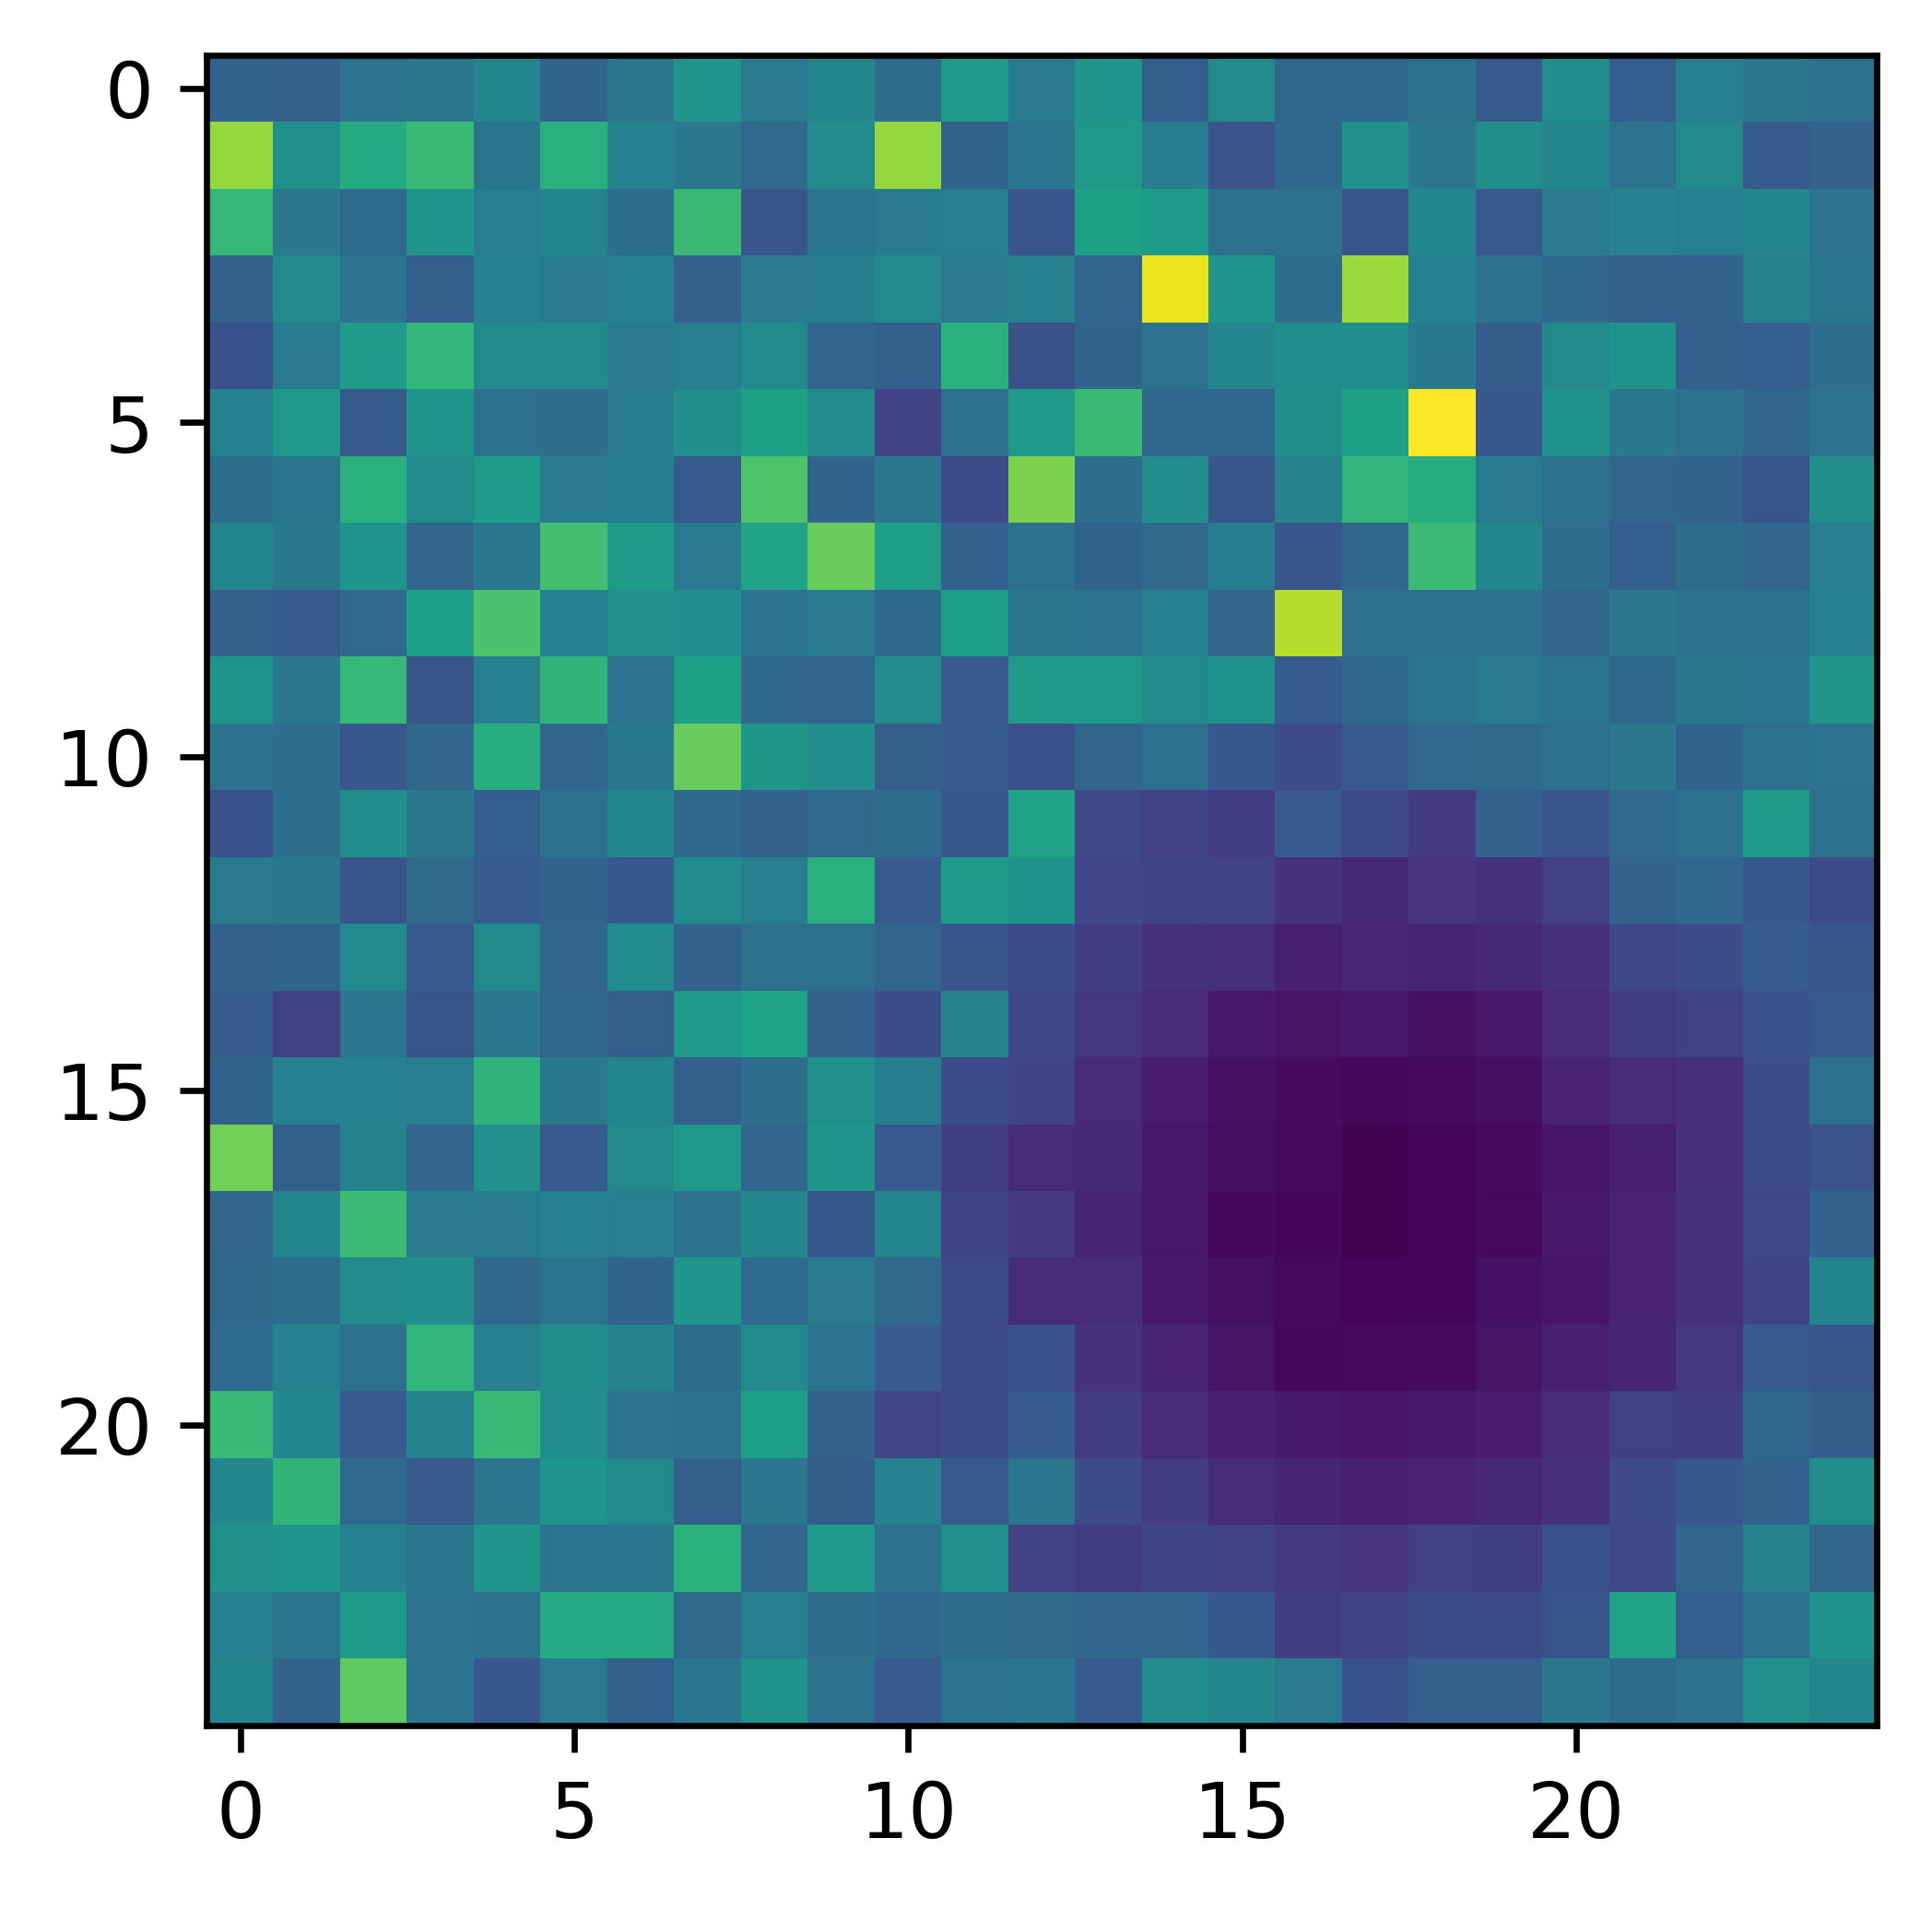
\includegraphics[width=\linewidth]{Graphics/guassian-2d-experiment-aprox.png}}\par 
	\subfigure[Coeficientes de detalle horizontal]{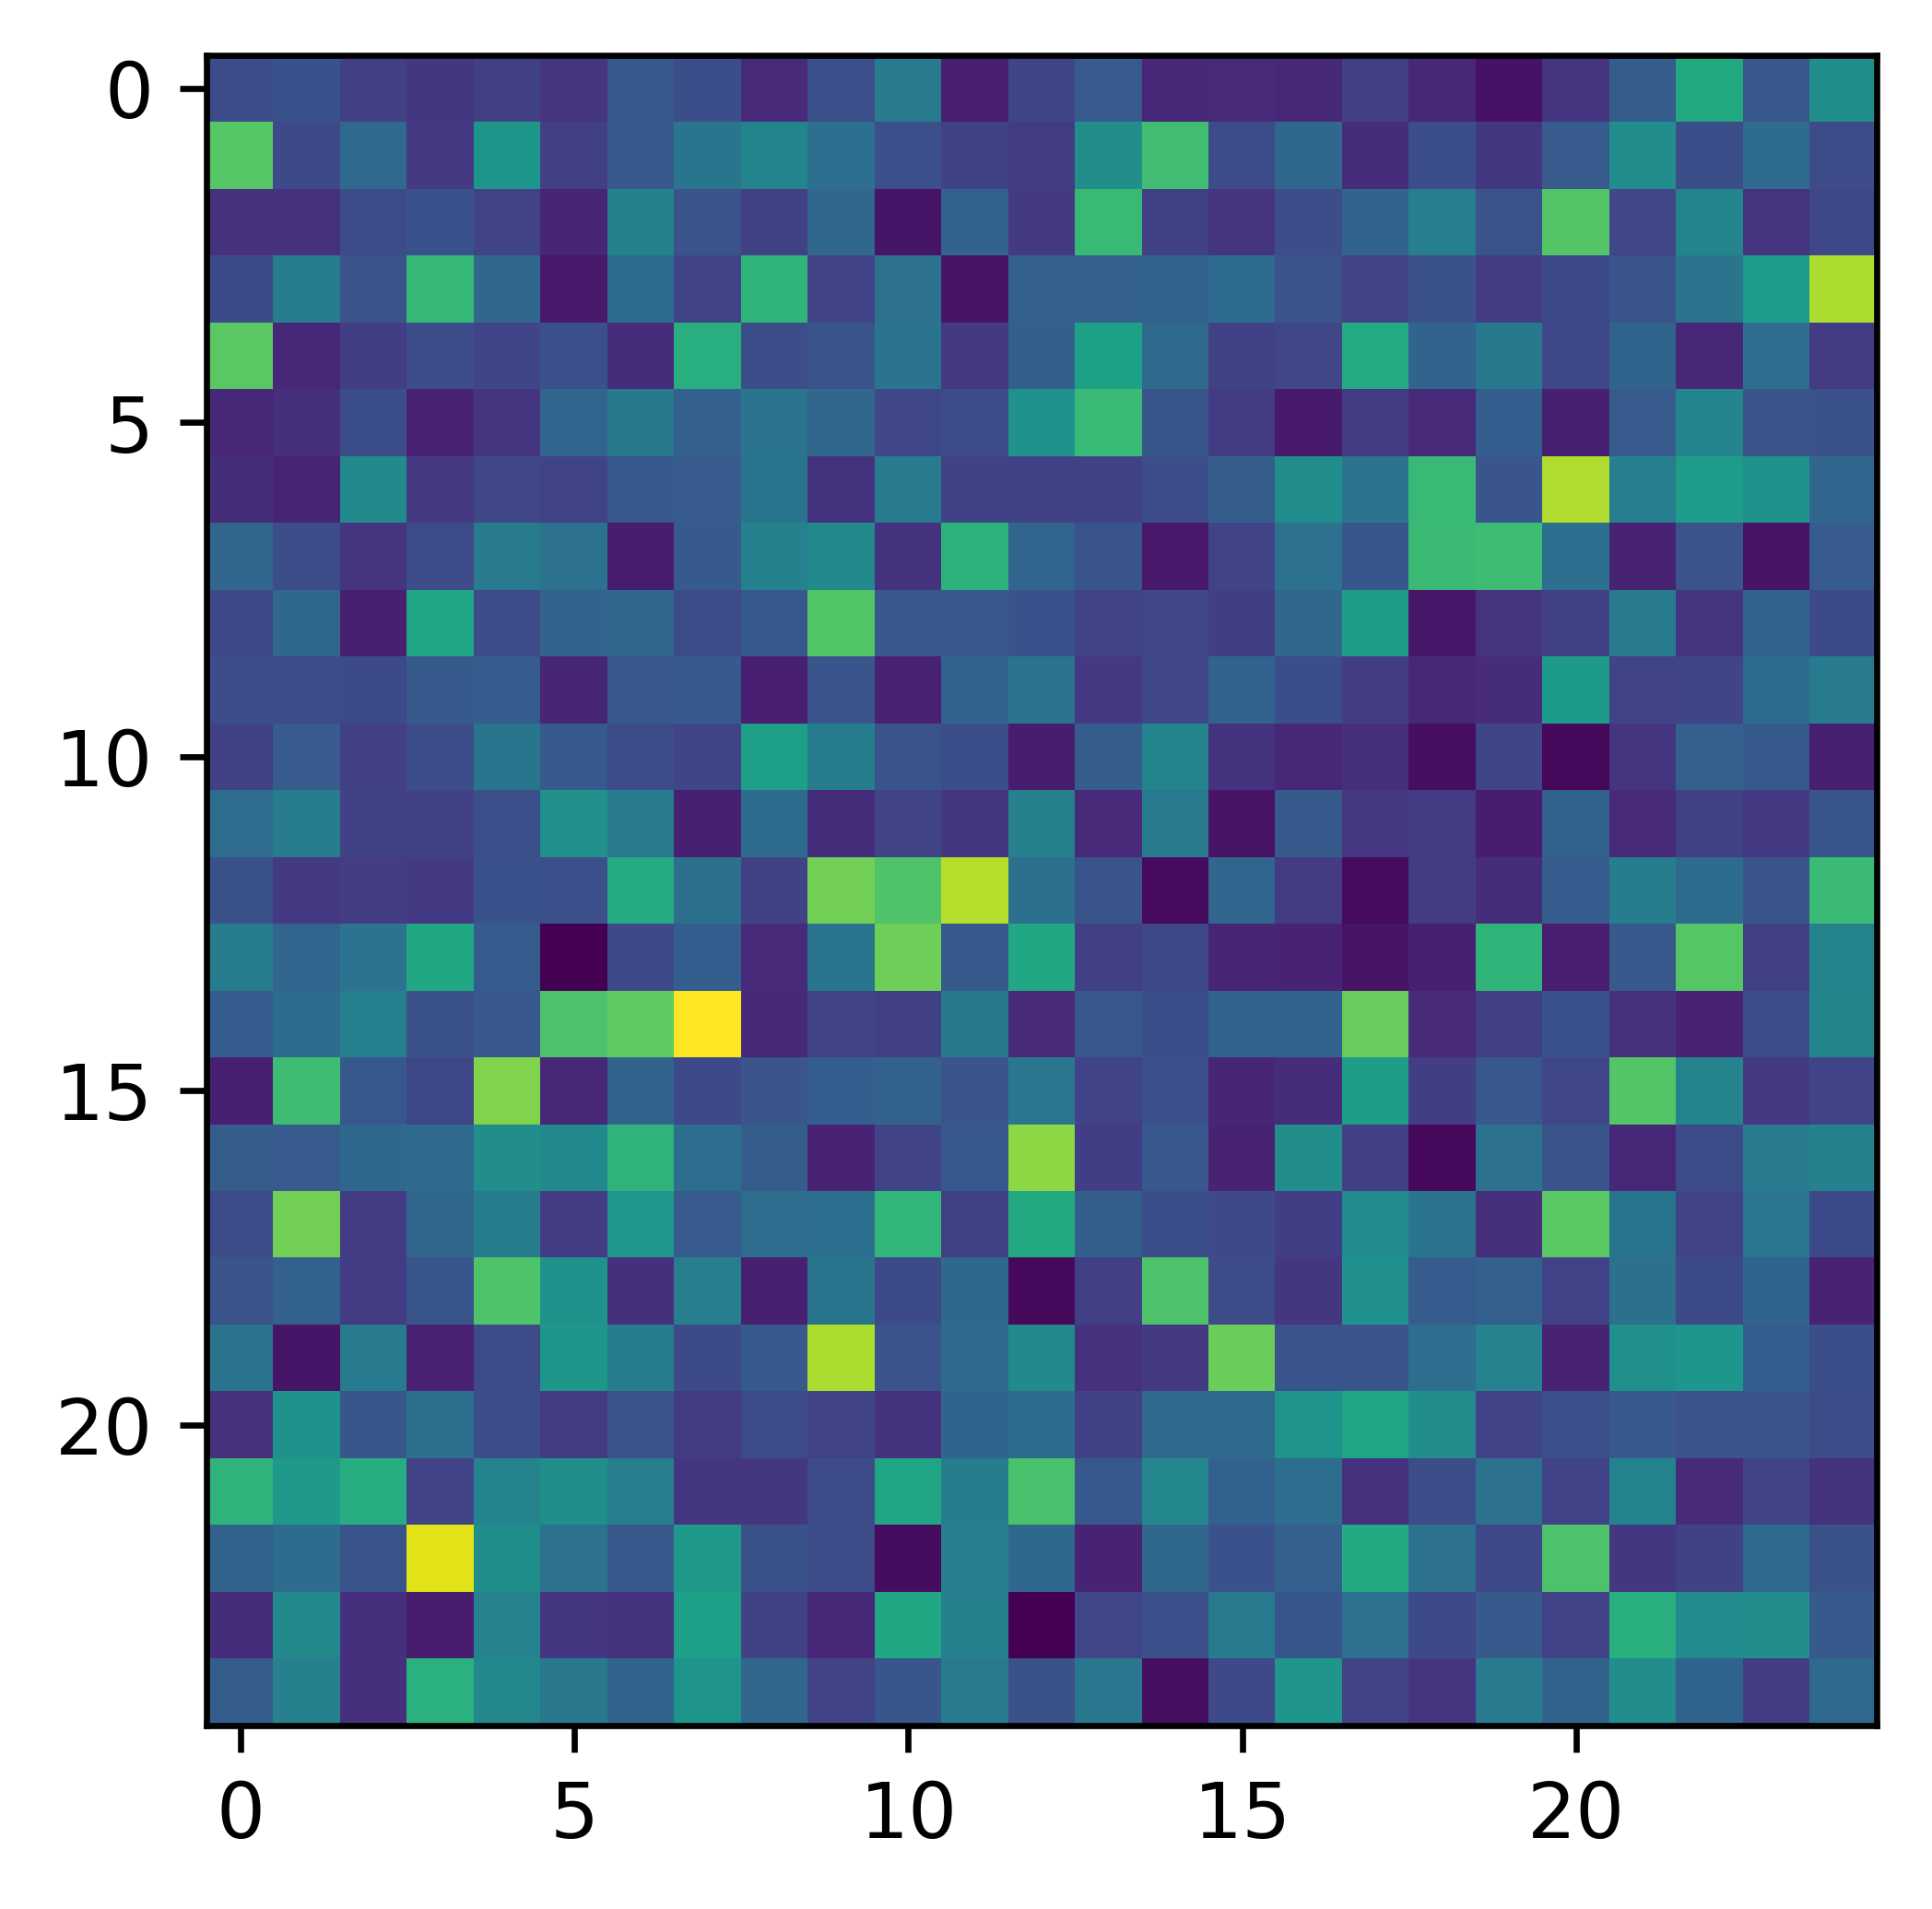
\includegraphics[width=\linewidth]{Graphics/gaussian-2d-experiment-horizontal.png}}\par 
    \end{multicols}
\begin{multicols}{2}
	\subfigure[Coeficientes de detalle vertical]{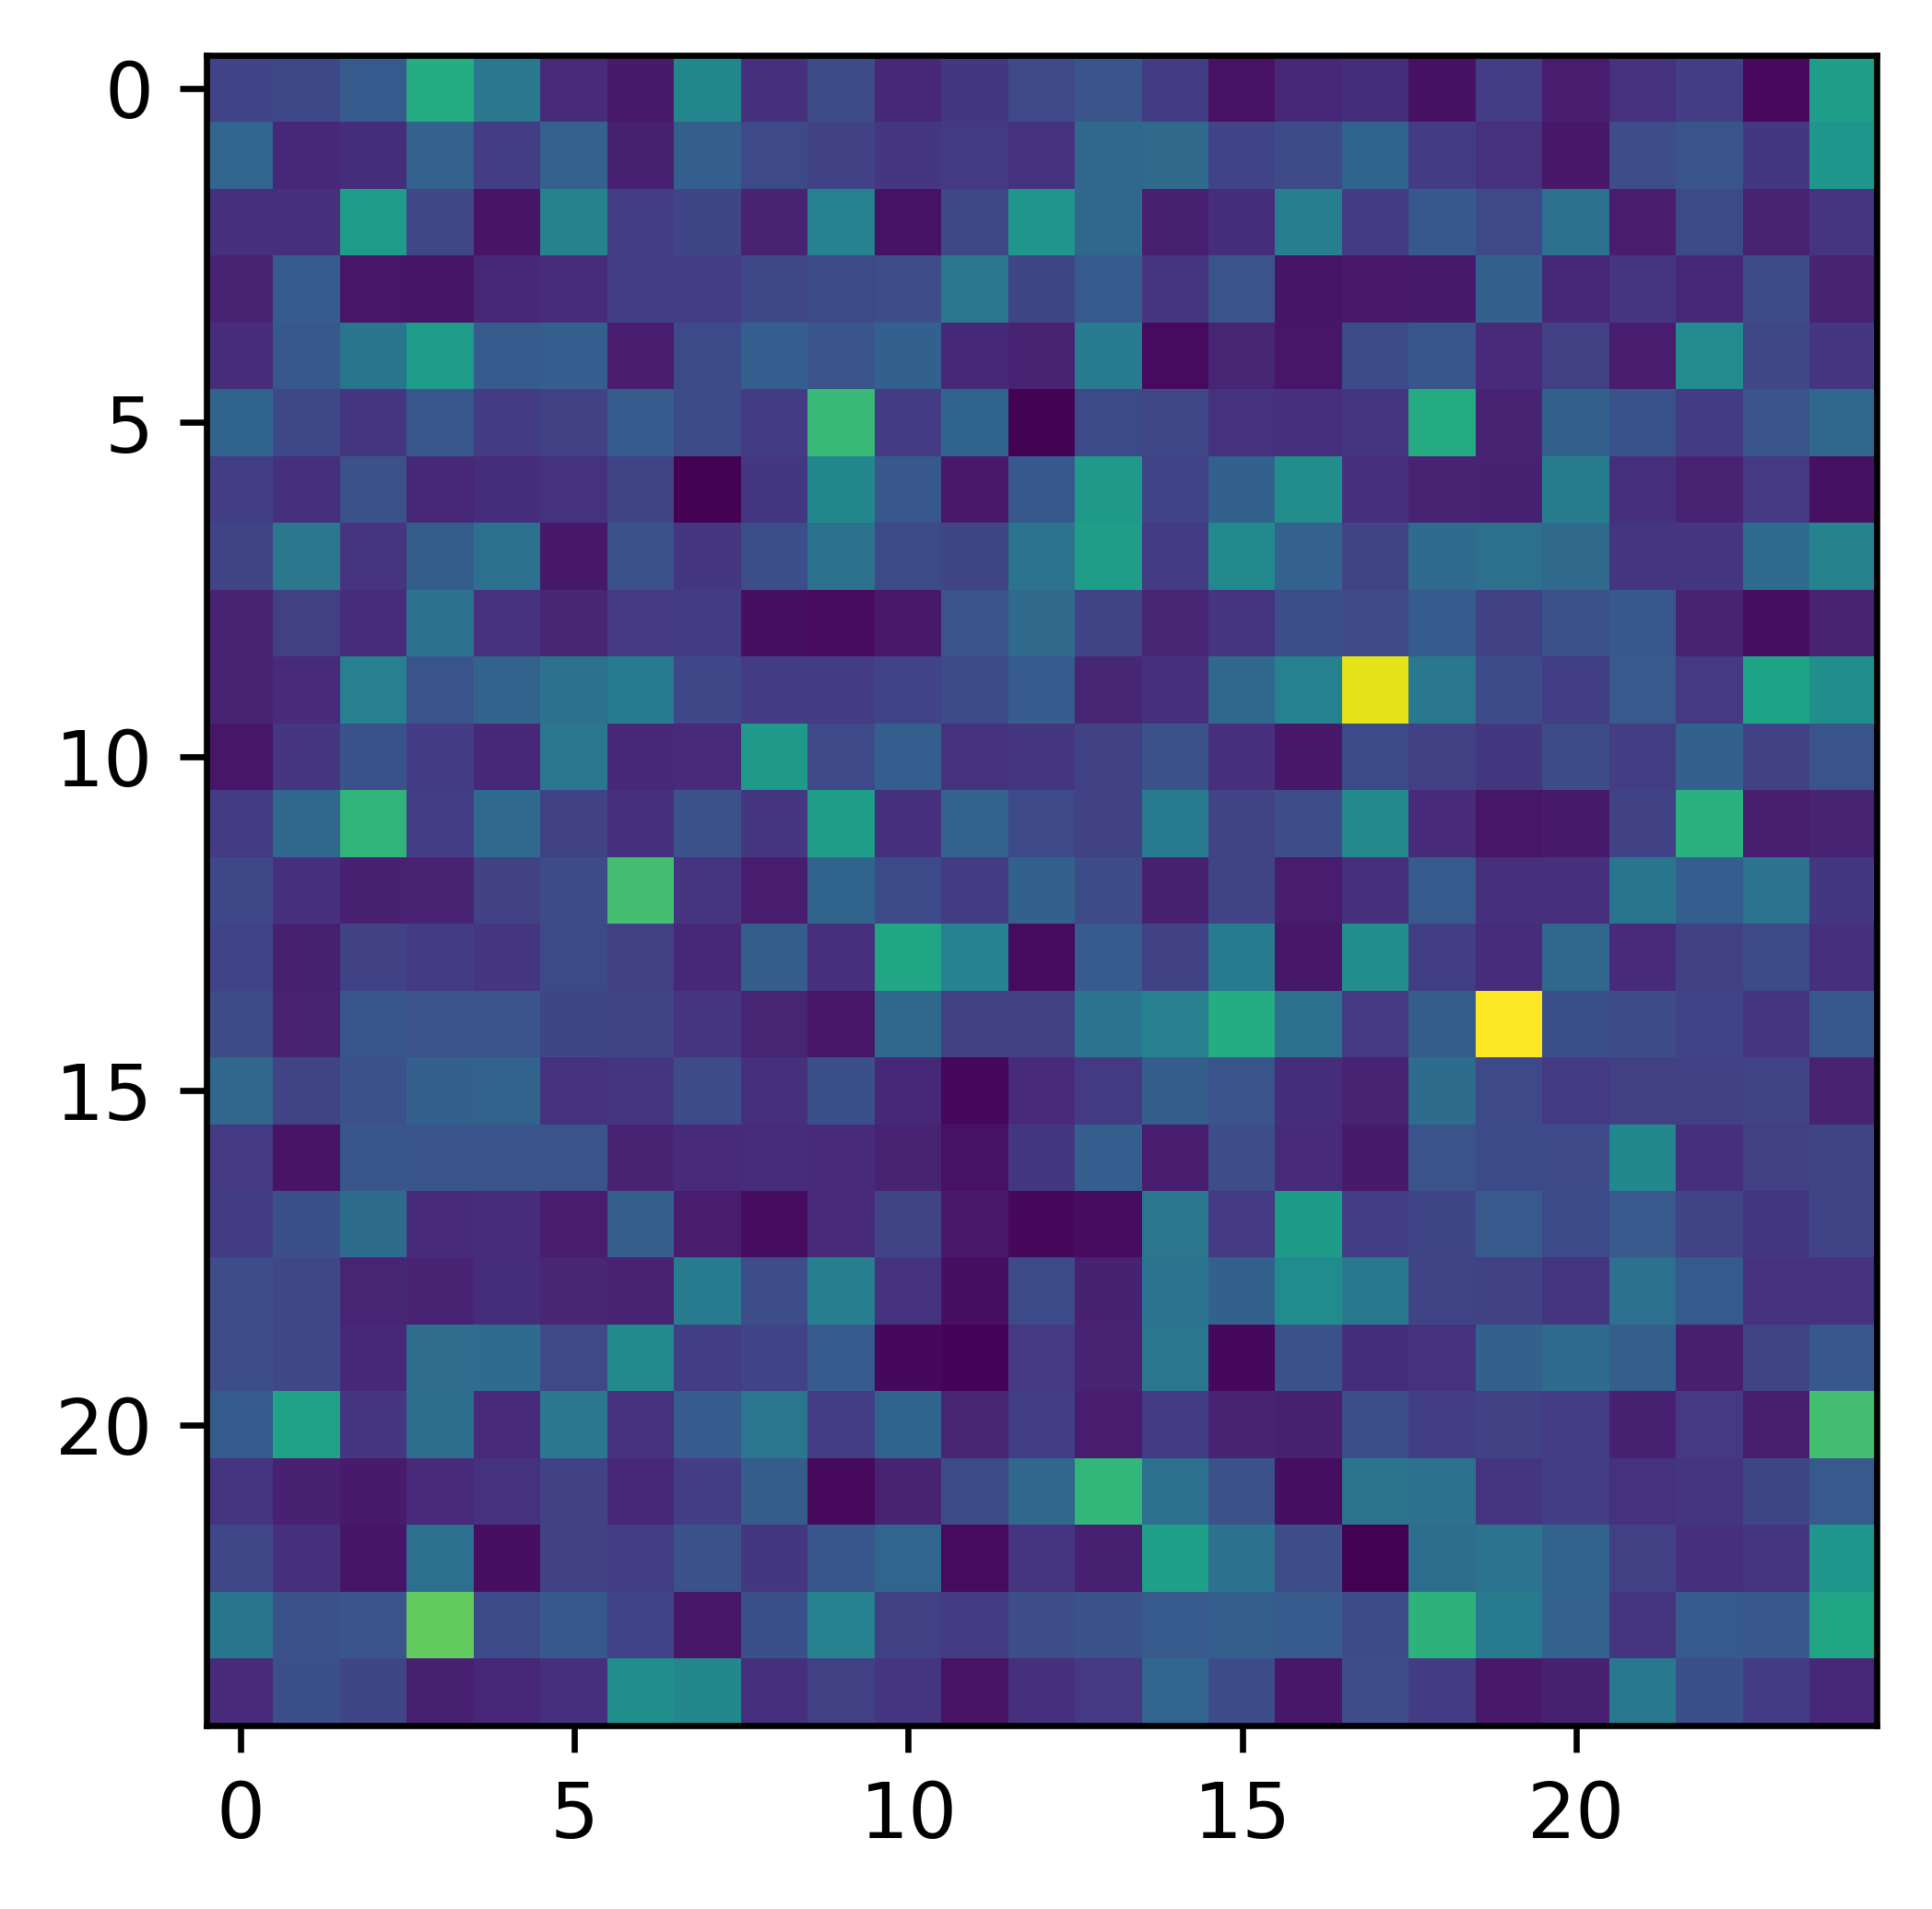
\includegraphics[width=\linewidth]{Graphics/gaussian-2d-experiment-vertical.png}}\par
	\subfigure[Coeficientes de detalle diagonal]{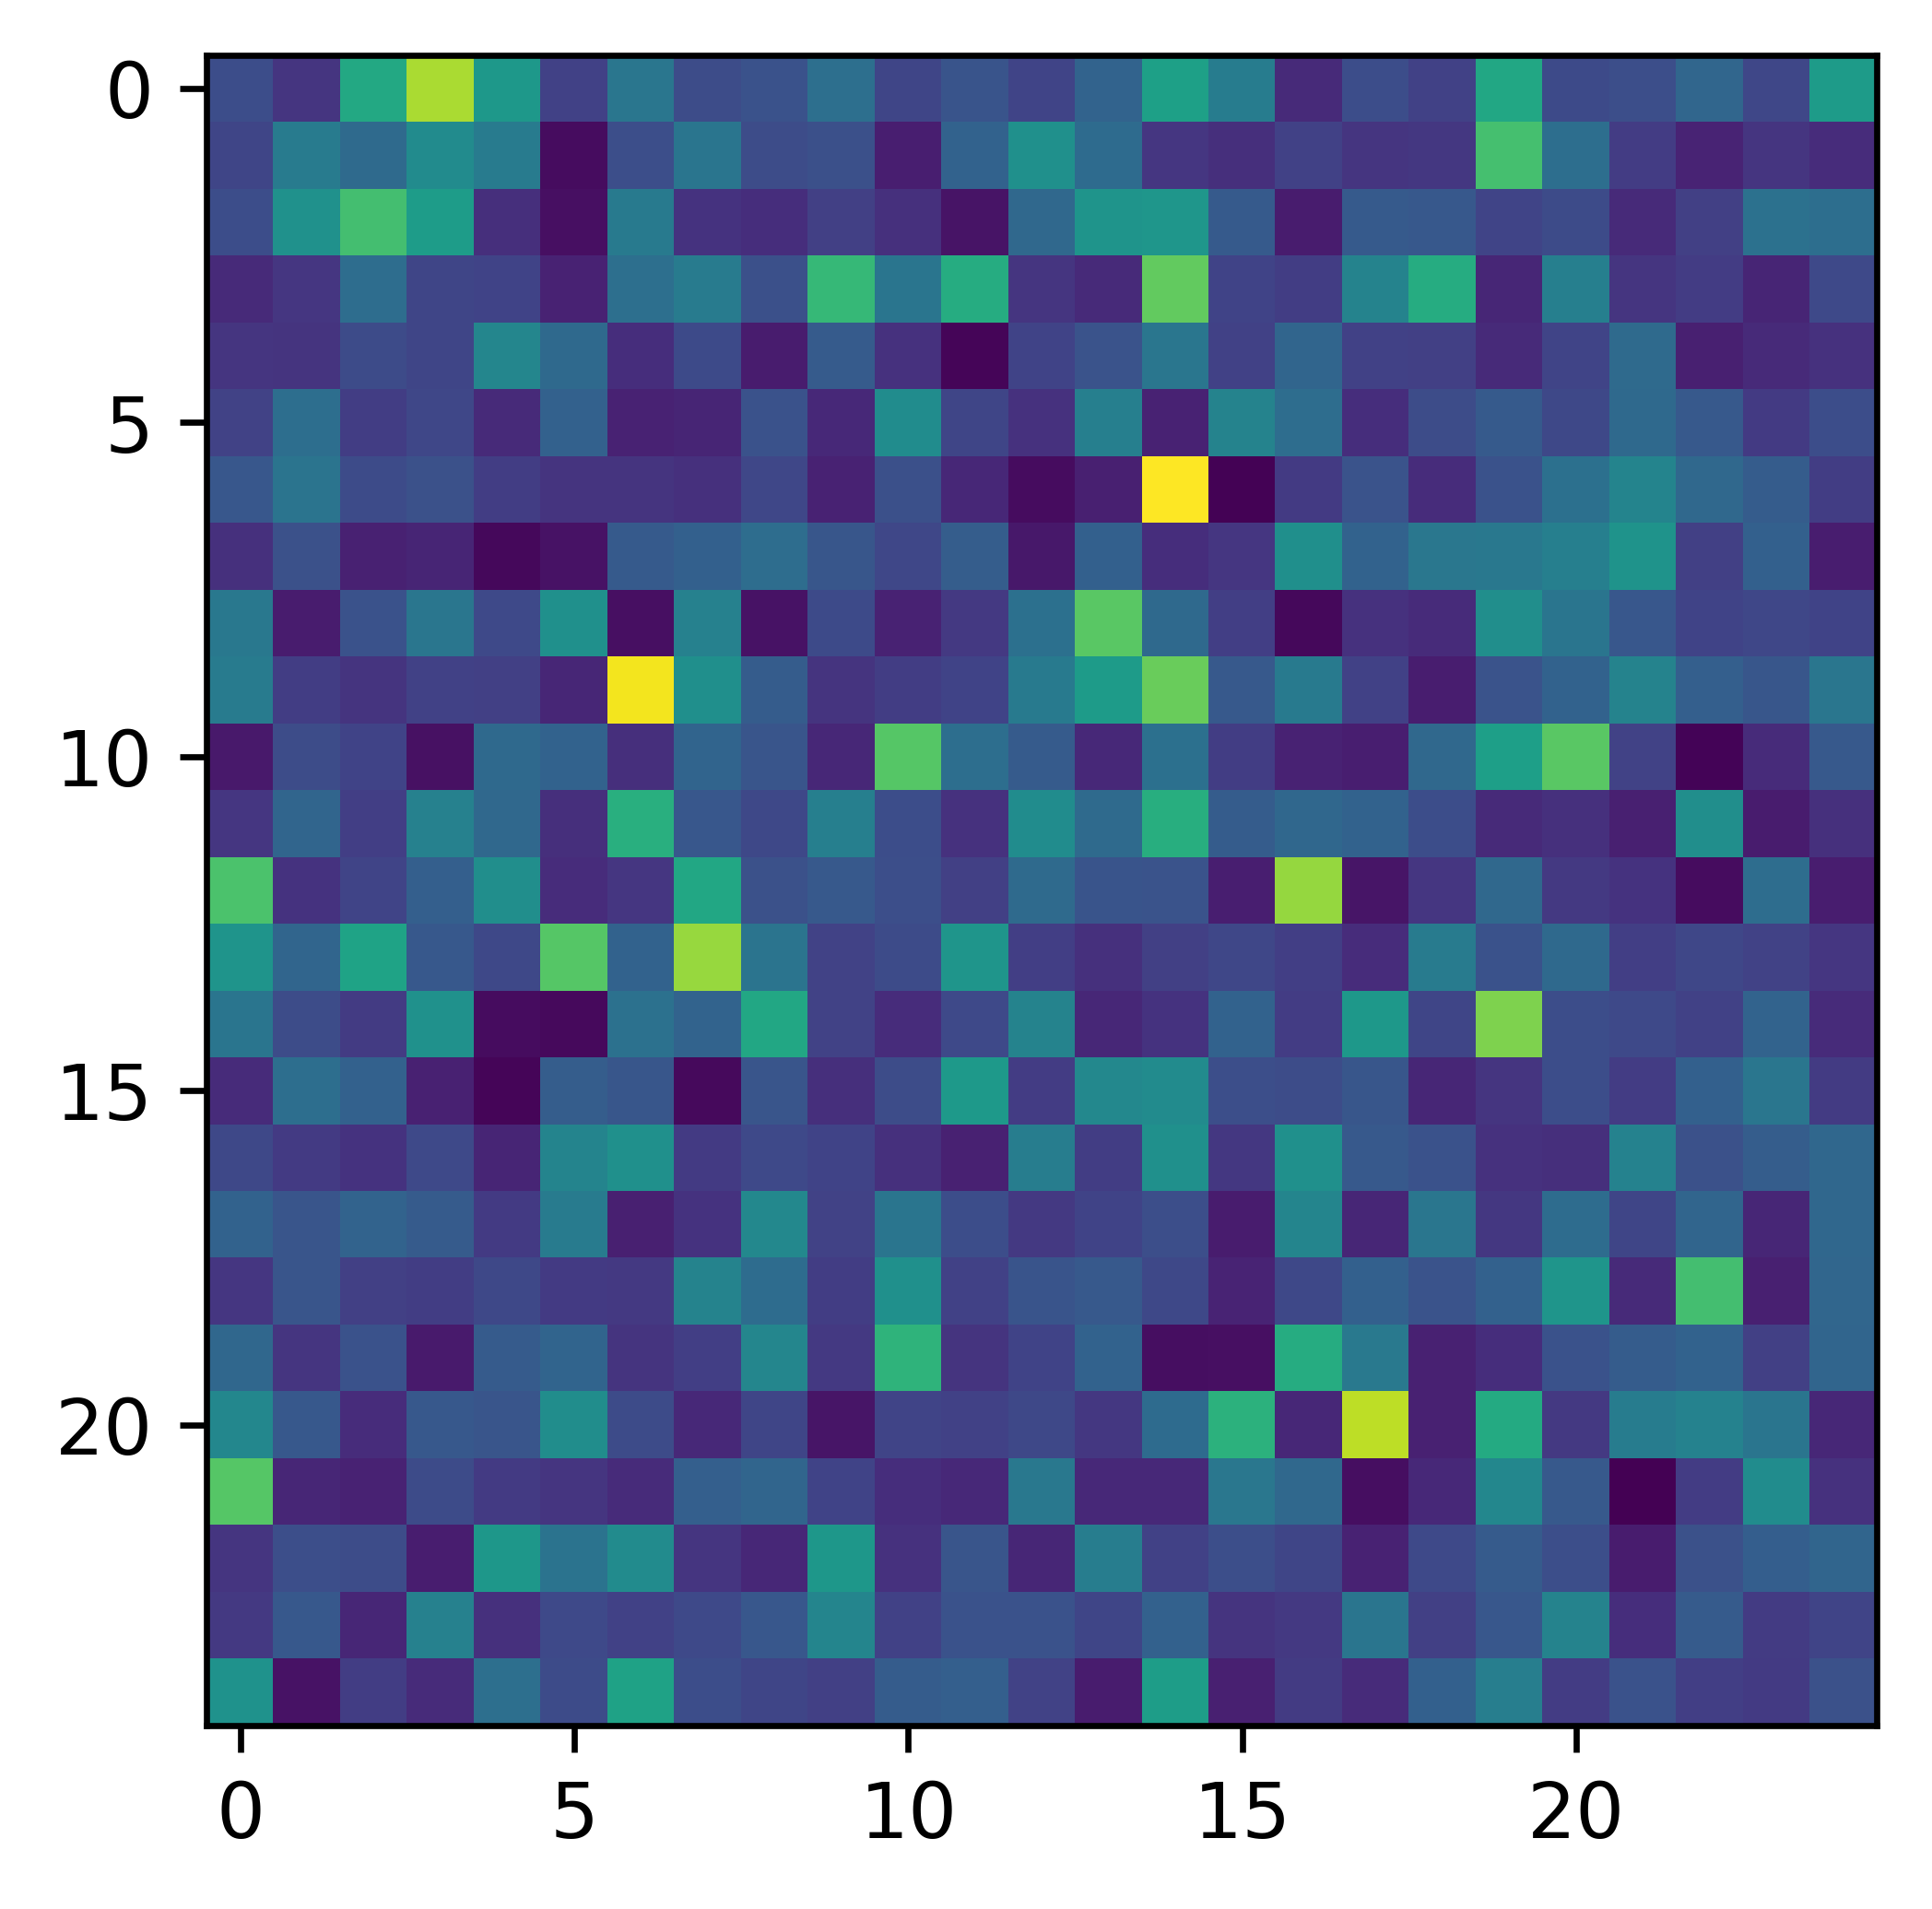
\includegraphics[width=\linewidth]{Graphics/gaussian-2d-experiment-diagonal.png}}\par
\end{multicols}
\caption{Resultado de evaluar $\mathbb{S}$ sobre cada uno de las componentes de la DST-II usando el primer enfoque} \label{fig:gaussian-example-approach1}
\end{figure*}


El resultado del segundo enfoque se aprecia en la Figura \ref{fig:gaussian-example-approach2}.
En este caso sí se puede apreciar claramente que existe un coeficiente que sobresale
entre los demás al realizar la DST-II por filas. El mismo se encuentra en la posición $(30,16)$ con un valor de $S=0.98$.
Esta posición corresponde aproximadamente al punto $(30,34)$ en la imagen original. Teniendo en cuenta que la
sección horizontal del patrón tomado está comprendida en el intervalo $[30,25:40]$, el resultado es bastante certero.

En el caso de la sección vertical, no se tuvo tanto éxito. No existe gran constraste entre ninguna posición con el resto. 
Esto se debe a que el error de las condiciones de detección es mucho mayor para la \textit{shapelet} de la sección
vertical que para la de la sección horizontal.

\begin{figure}
	\centering
	\subfigure[Por filas]{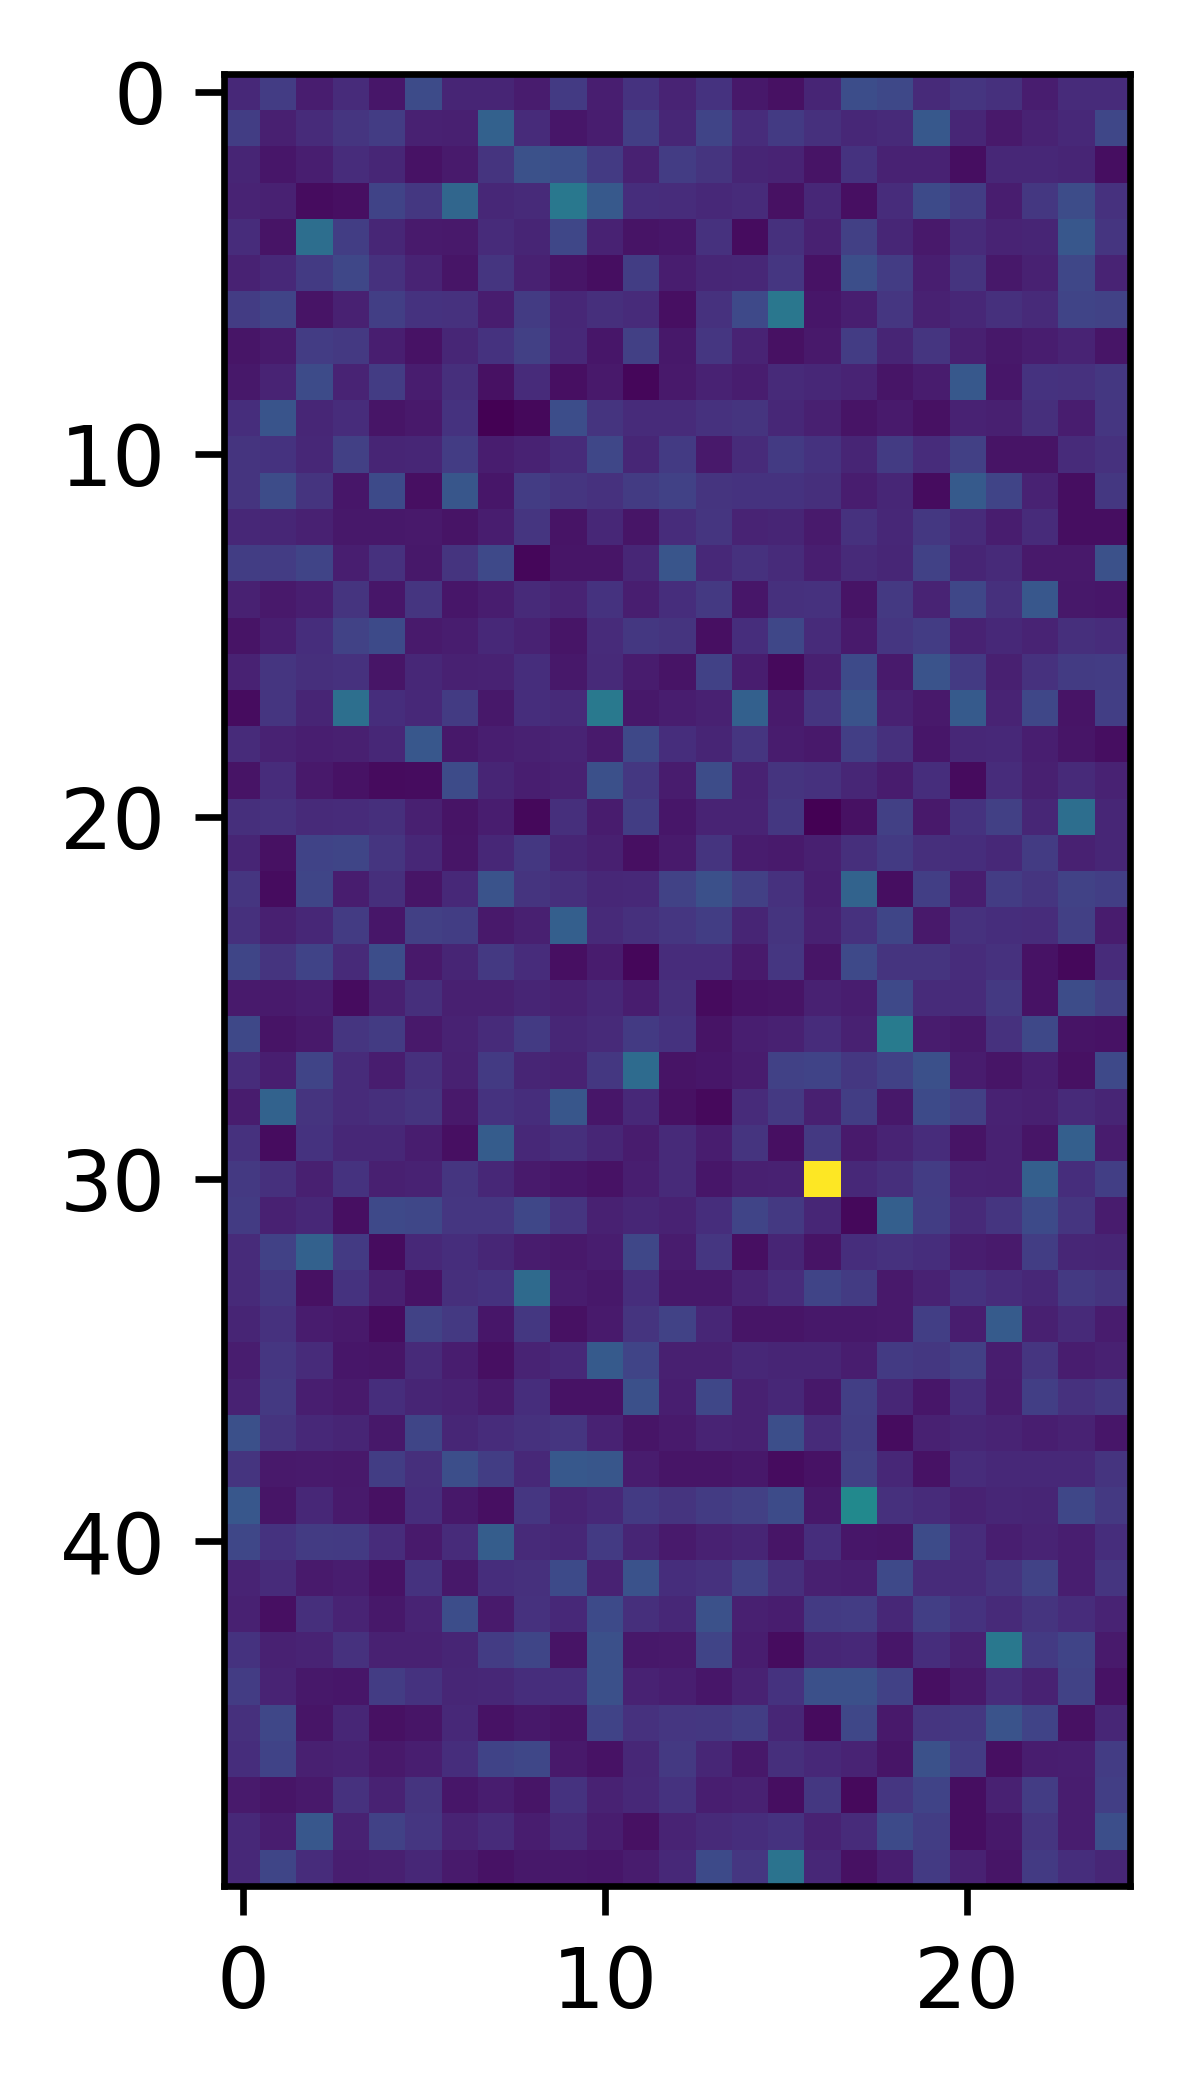
\includegraphics{Graphics/gaussian-2d-experiment2-row.png}}
	\subfigure[Por columnas]{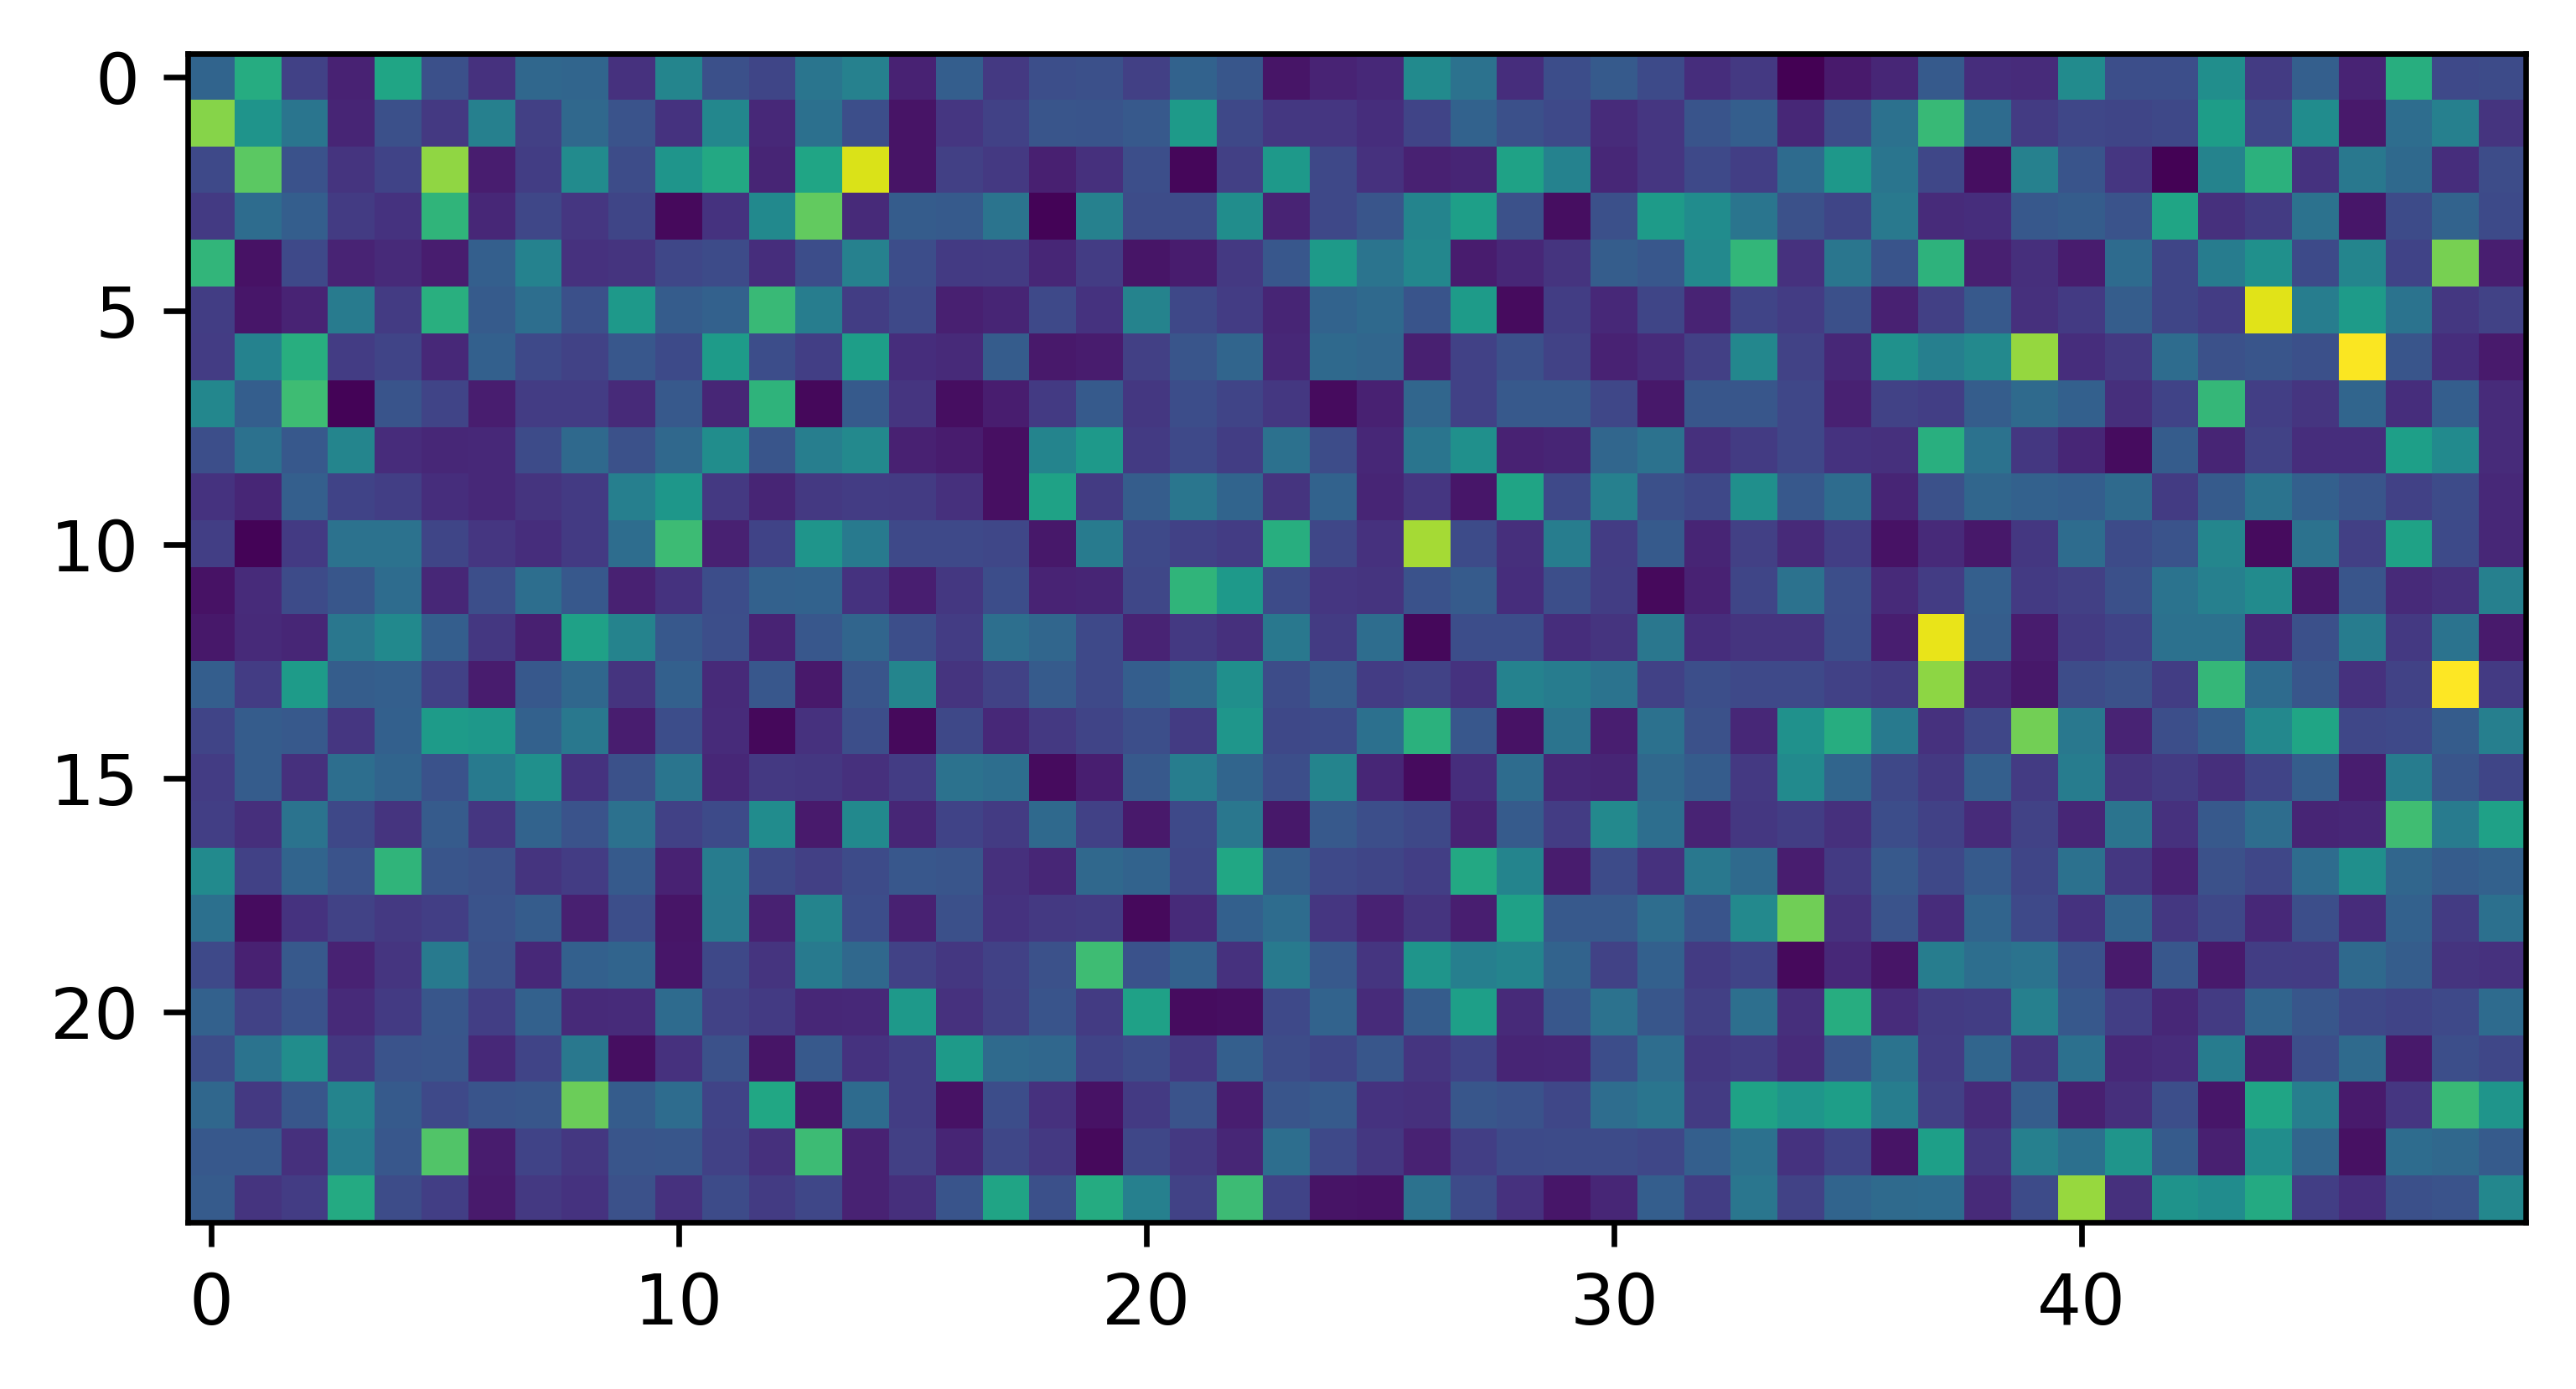
\includegraphics{Graphics/gaussian-2d-experiment2-col.png}}
	\caption{Resultado de evaluar $\mathbb{S}$ sobre cada una de las \textit{second-rated} de la DST-II usando el segundo enfoque.} \label{fig:gaussian-example-approach2}
\end{figure}
%-0.00781404414483181 col error matching
%0.0118491040034377
%-2.61711684291969e-18 row error matchine
%-8.05175395622083e-18

En el caso del tercer enfoque, se toma la región comprendida entre los píxeles $[25:40,25:40]$. Los resultados 
se muestran en la Figura \ref{fig:gaussian-example-approach3}. En este caso, se logra obtener toda una región con mayor 
contraste que corresponde aproximadamente a las posiciones donde se encuentra el patrón. 
Sin embargo, muchos de estos valores realmente no sobrepasan el umbral $0.7$,
por el hecho de que una parte de los filtros calculados tienen errores altos en las condiciones de detección, 
por lo que no detectan bien su sección del patrón correspondiente y al promediar los resultados introducen 
ruido en el resultado final.
Esto limita considerablemente la capacidad de detectar una región entera usando este enfoque. Otra desventaja es el costo
computacional. Resolver varios sistemas de ecuaciones no lineales puede tomar bastante tiempo, sobre todo si las 
muestras son grandes.

\begin{figure}
	\centering
	\subfigure[Por filas]{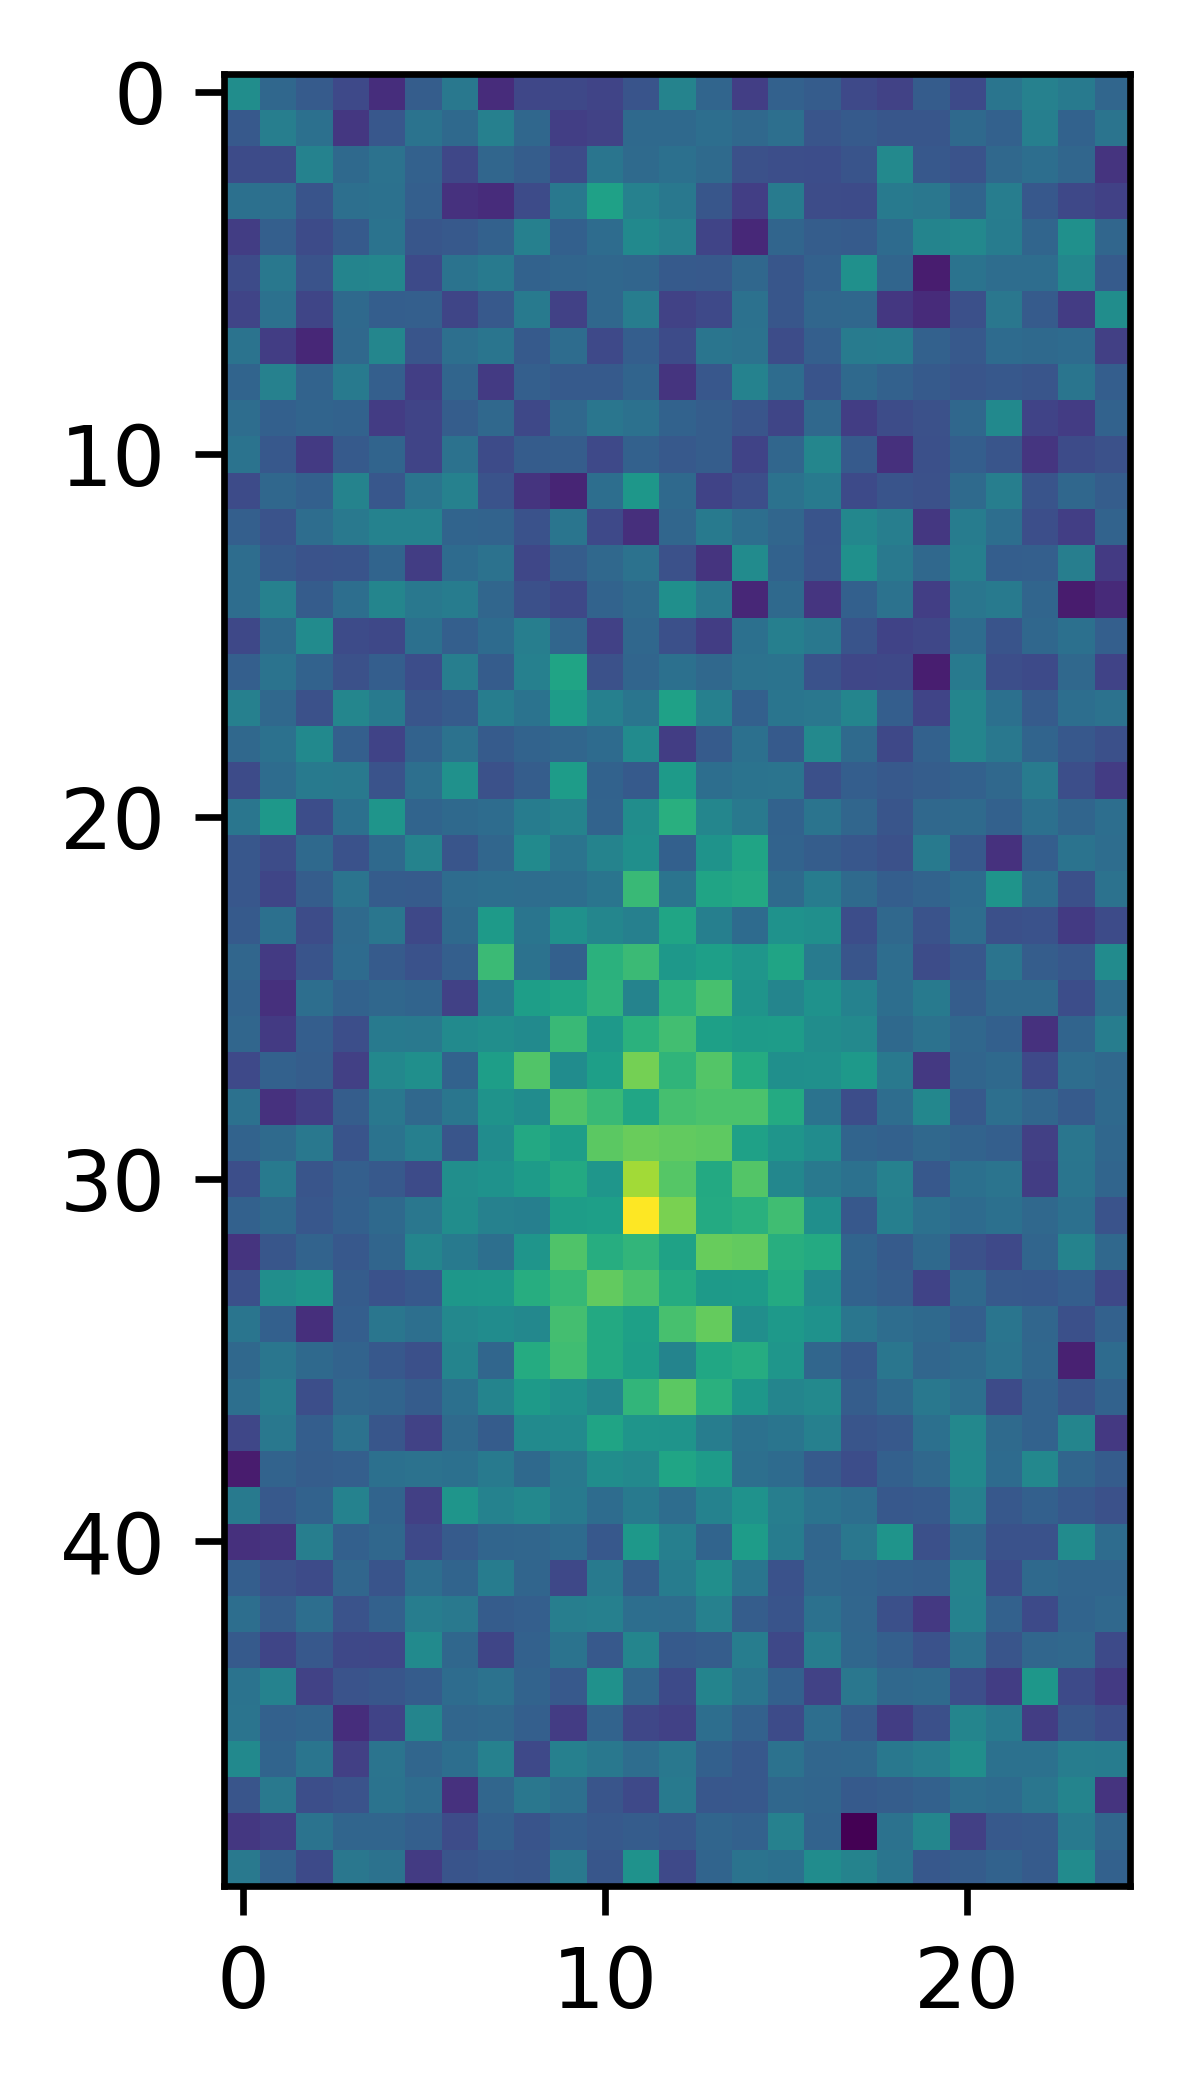
\includegraphics{Graphics/gaussian-2d-experiment3-row.png}}
	\subfigure[Por columnas]{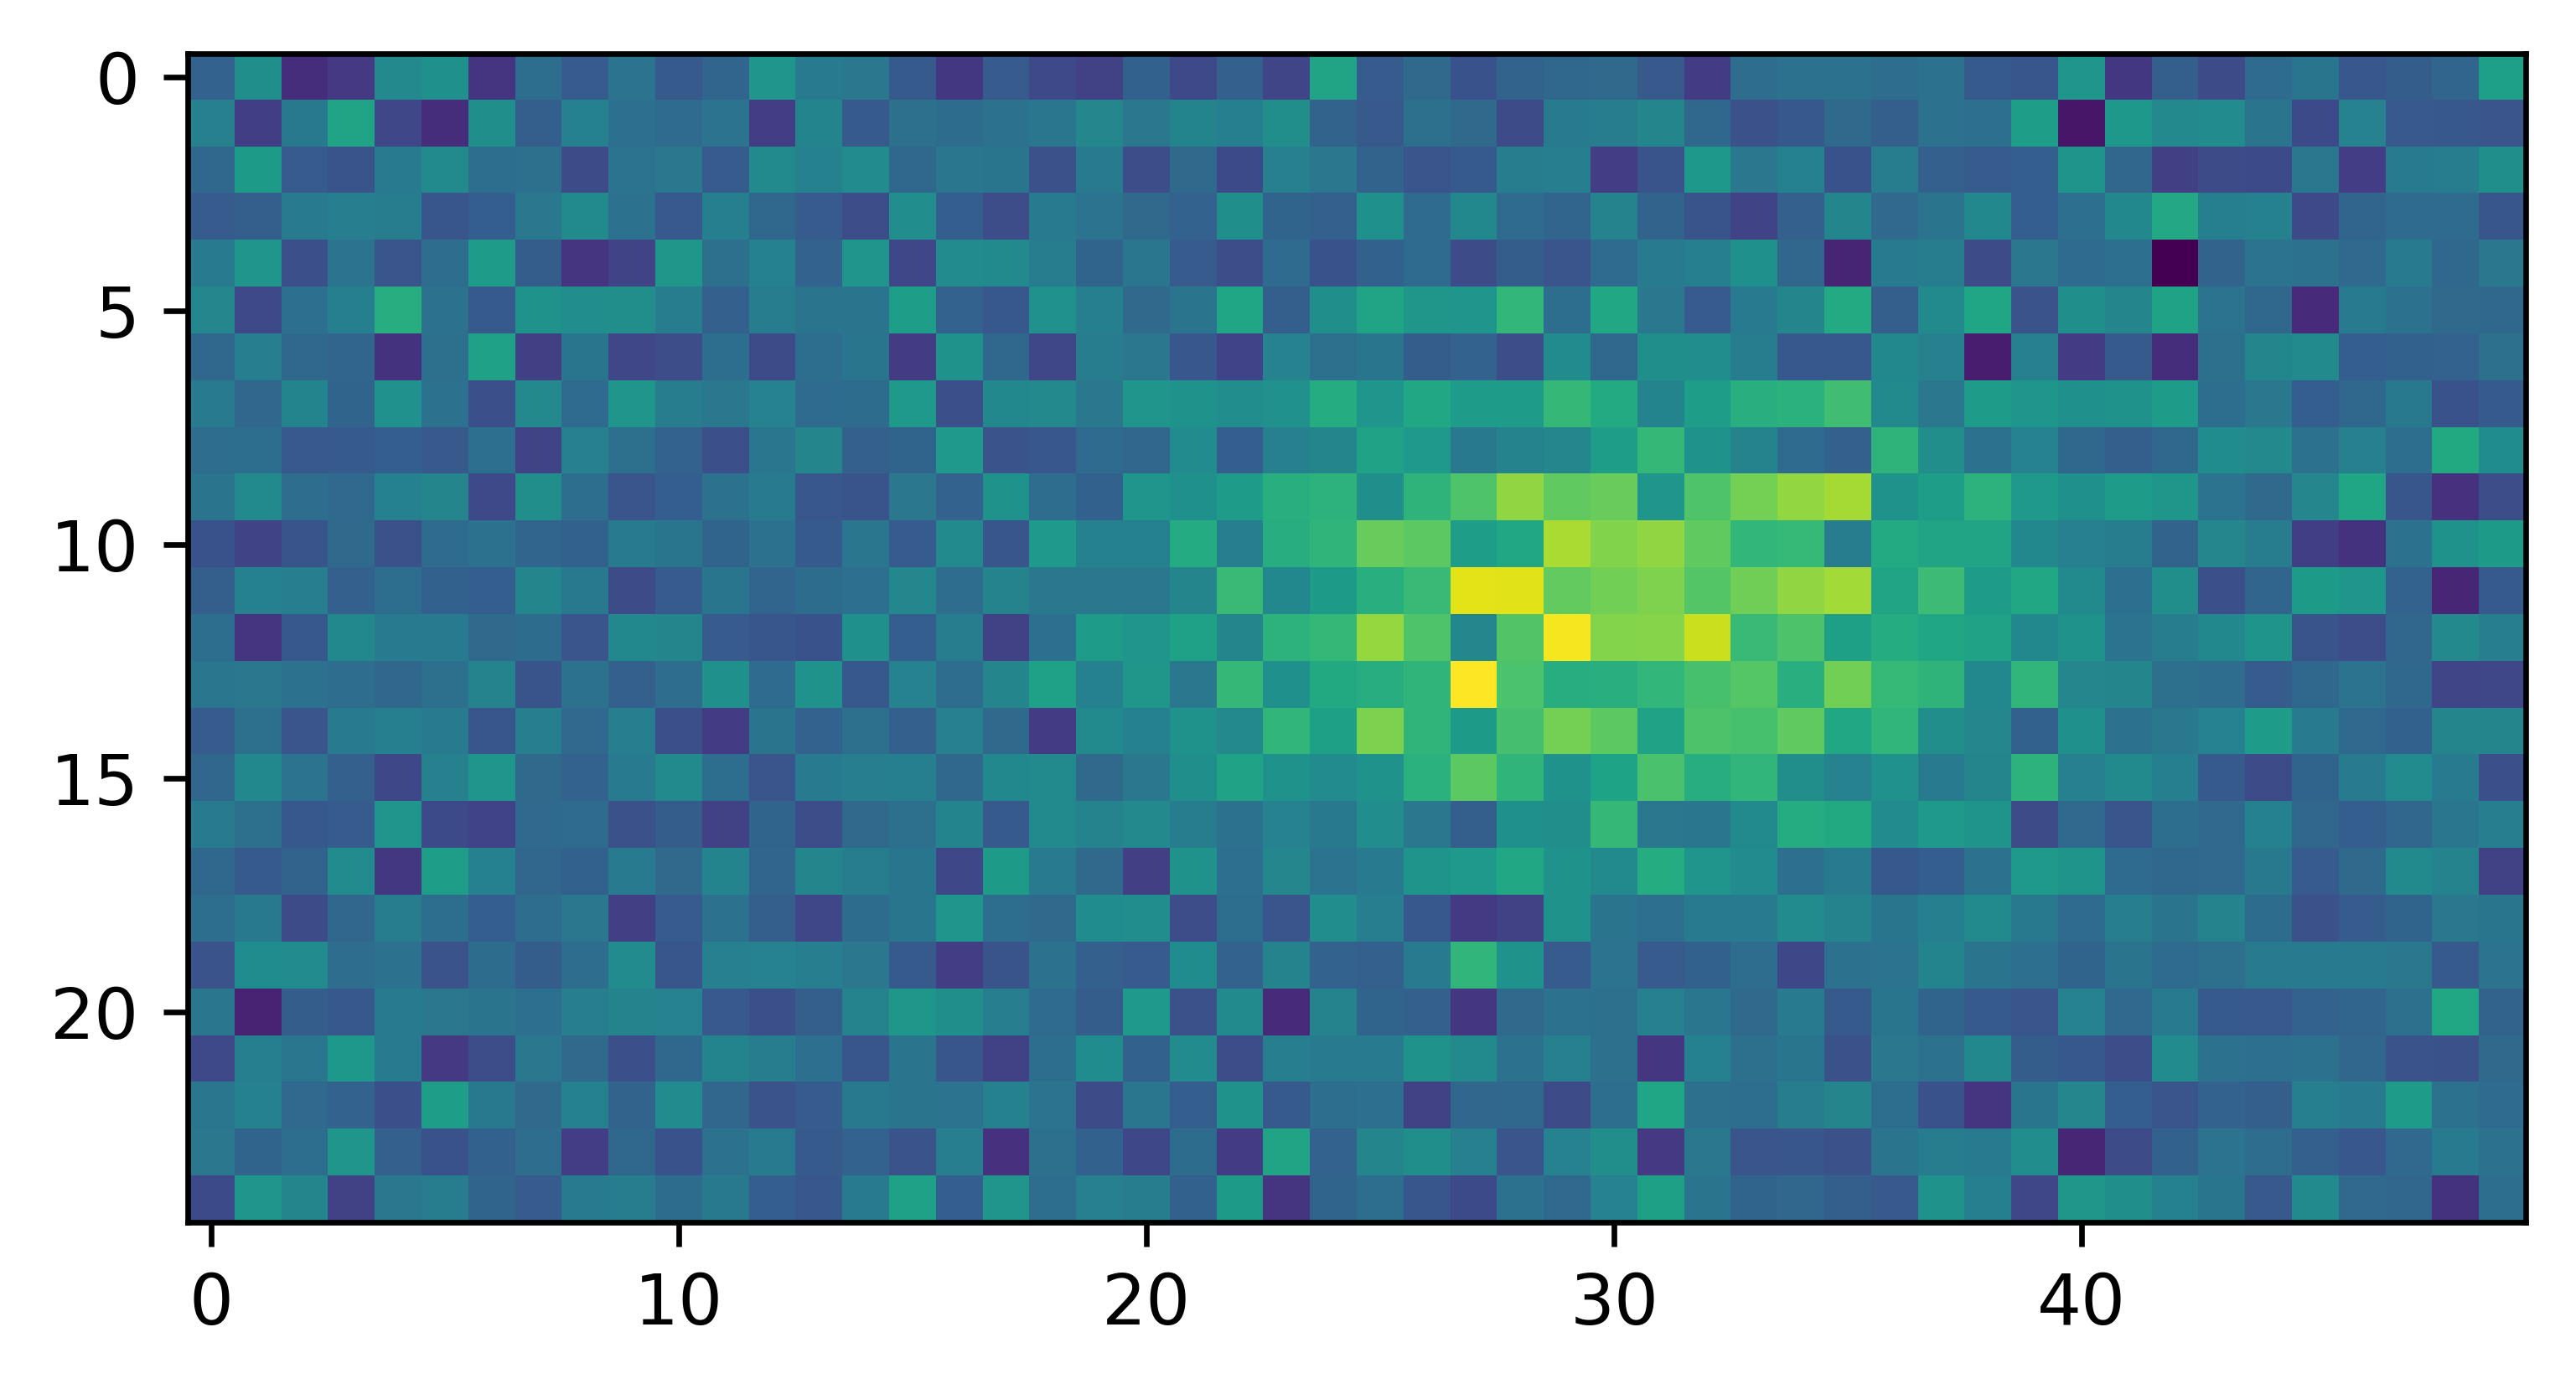
\includegraphics{Graphics/gaussian-2d-experiment3-col.png}}
	\caption{Resultado de evaluar $\mathbb{S}$ sobre cada una de las \textit{second-rated} de la DST-II usando el tercer enfoque.} \label{fig:gaussian-example-approach3}
\end{figure}

\section{Applicación en la detección de masas en mamografías}

Para evaluar la capacidad del algoritmo de la DST-II y las propuestas de extensión al caso bidimensional en
la detección de masas de mamografías se usó la base de datos INBreast \cite{Moreira2012}. La misma 
contiene un total de 115 casos (410 imágenes), todas con anotaciones sobre distintos tipos de lesiones. 
En este caso, son de interés las de tipo masas, específicamente las que presentan isotropía.

Las imágenes poseen una resolución de $3328\times 4084$ o $2560\times 3328$ y están guardadas en formato
DICOM. Para su lectura se usó el paquete Pydicom \cite{darcy_mason_2020_4313150}.

Dado que las imágenes tienen una resolución alta se realiza un pre-procesamiento antes de aplicar el
algoritmo. Como primer paso, se realiza un reescalado de las imágenes. Para esto se usa la función de scikit-image
\textit{skimage.transform.rescale} con un factor de $\frac{1}{8}$ \cite{skimage-transform}. Luego de este reescalado,
se realiza un suavizado a la imagen y un \textit{sharpening}. El primero se realiza con un filtro guassiano
para eliminar la existencia de ruido en la mamografía. Para el segundo se usa un filtro laplaciano con el objetivo
de detectar mejor los bordes. Ambos resultados se fusionan y sobre esa imagen se aplica el algoritmo.

A continuación se muestra un ejemplo de los experimentos realizados.

\subsection{Ejemplos de los experimentos y análisis de los resultados}

El ejemplo tomado se muestra en la Figura \ref{fig:example-mm}. La imagen muestra los resultados de cada etapa 
del preprocesamiento: reescalado, filtro gaussiano, filtro laplaciano y, por último, fusión de los
resultados de ambos filtros.

\begin{figure*}
	\begin{multicols}{2}
		\subfigure[Reescalado]{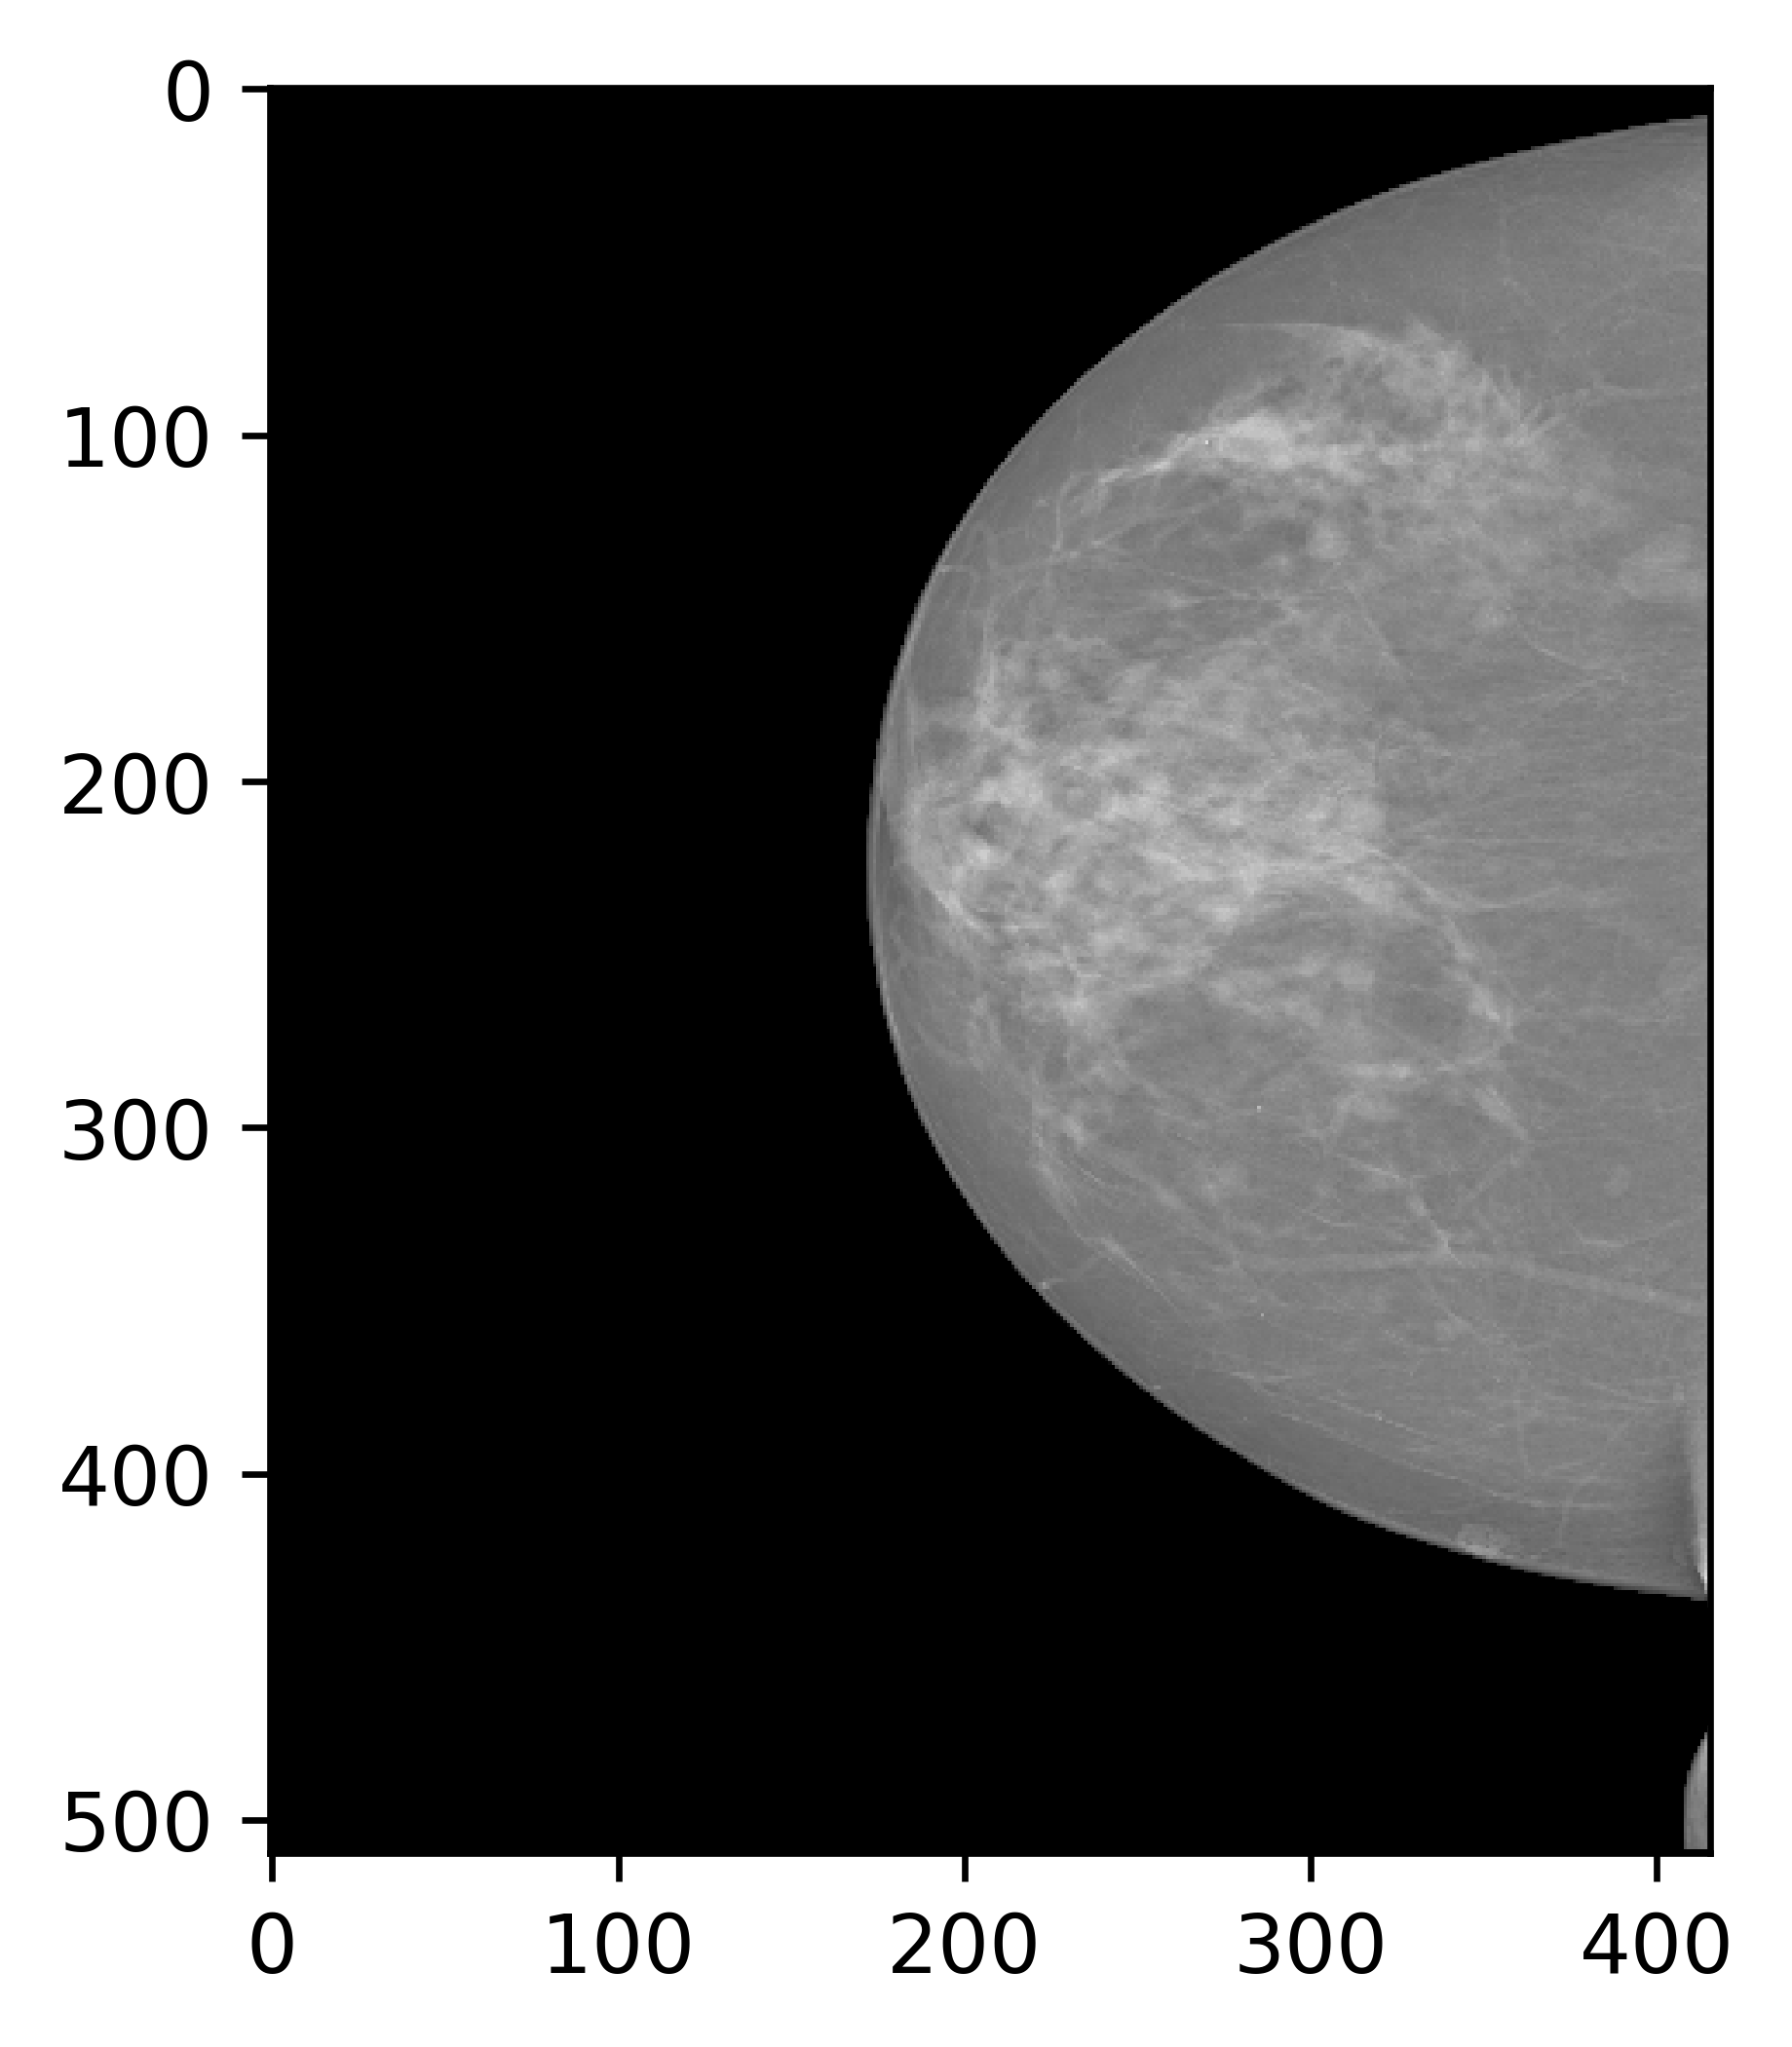
\includegraphics[scale=0.9]{Graphics/mm-rescaled.png}}\par
		\subfigure[Filtro gaussiano]{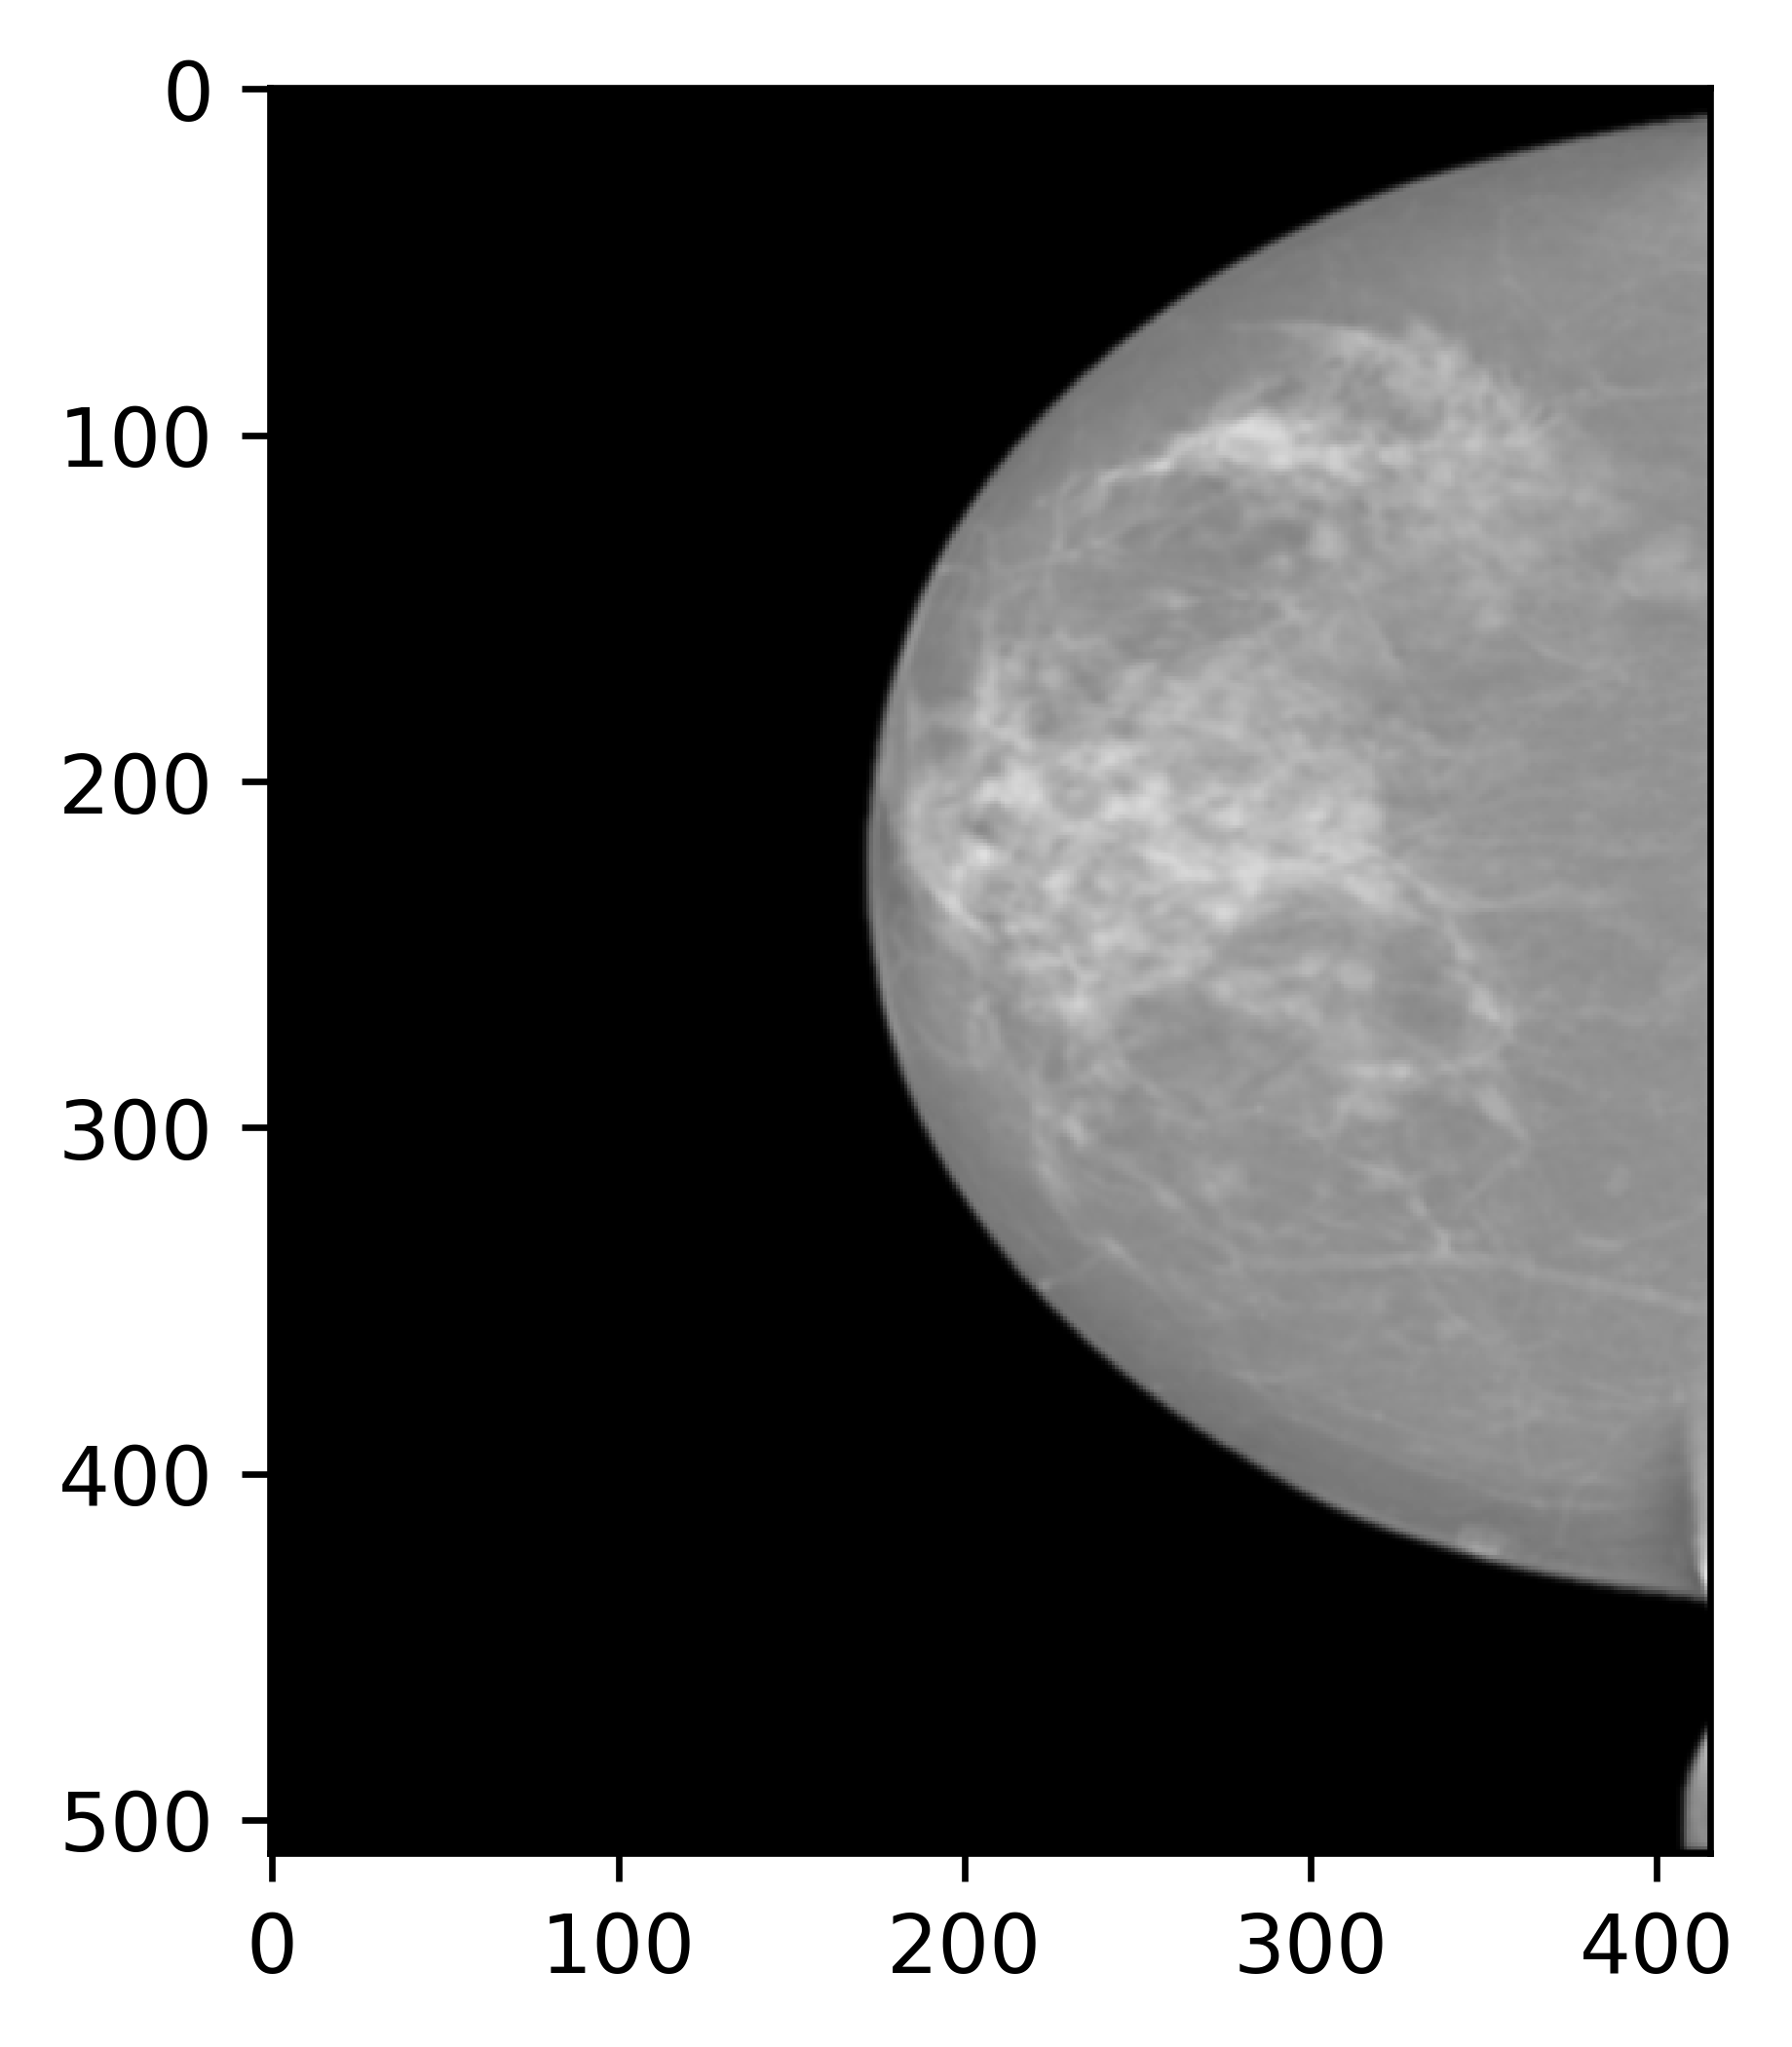
\includegraphics[scale=0.9]{Graphics/mm-smooth.png}}\par
		\end{multicols}
	\begin{multicols}{2}
		\subfigure[Filtro laplaciano]{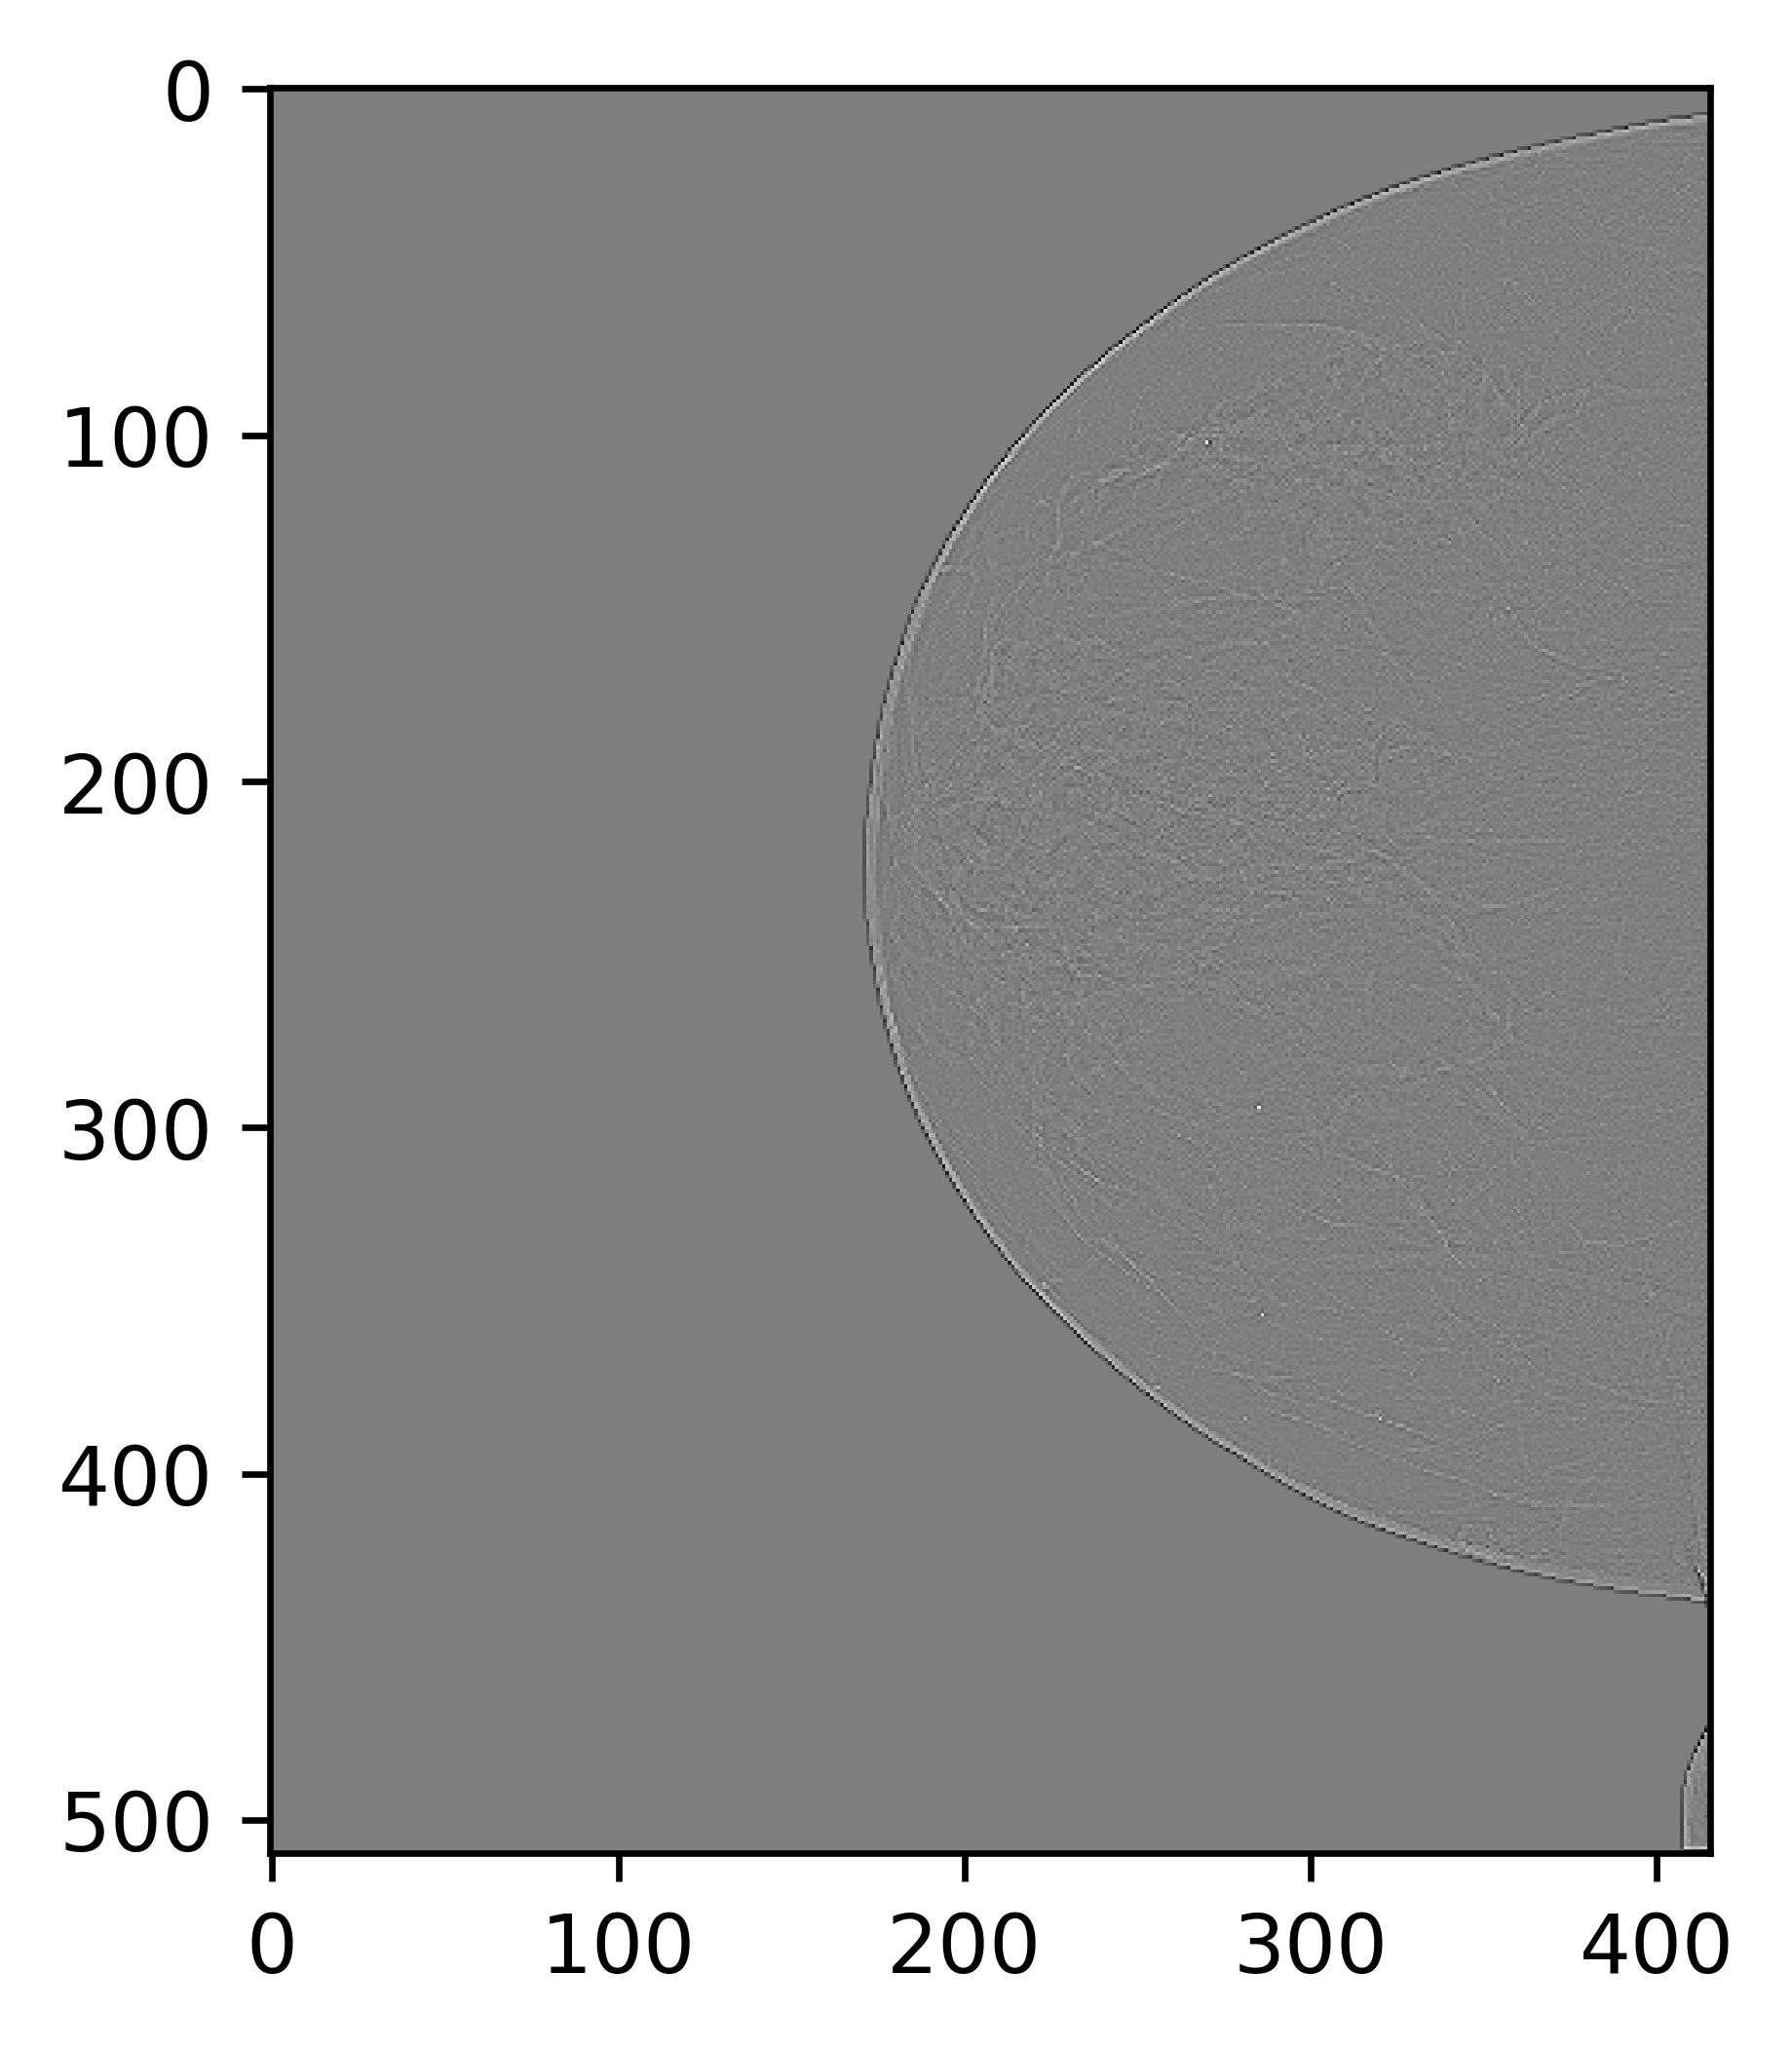
\includegraphics[scale=0.9]{Graphics/mm-sharp.png}}\par
		\subfigure[Fusión]{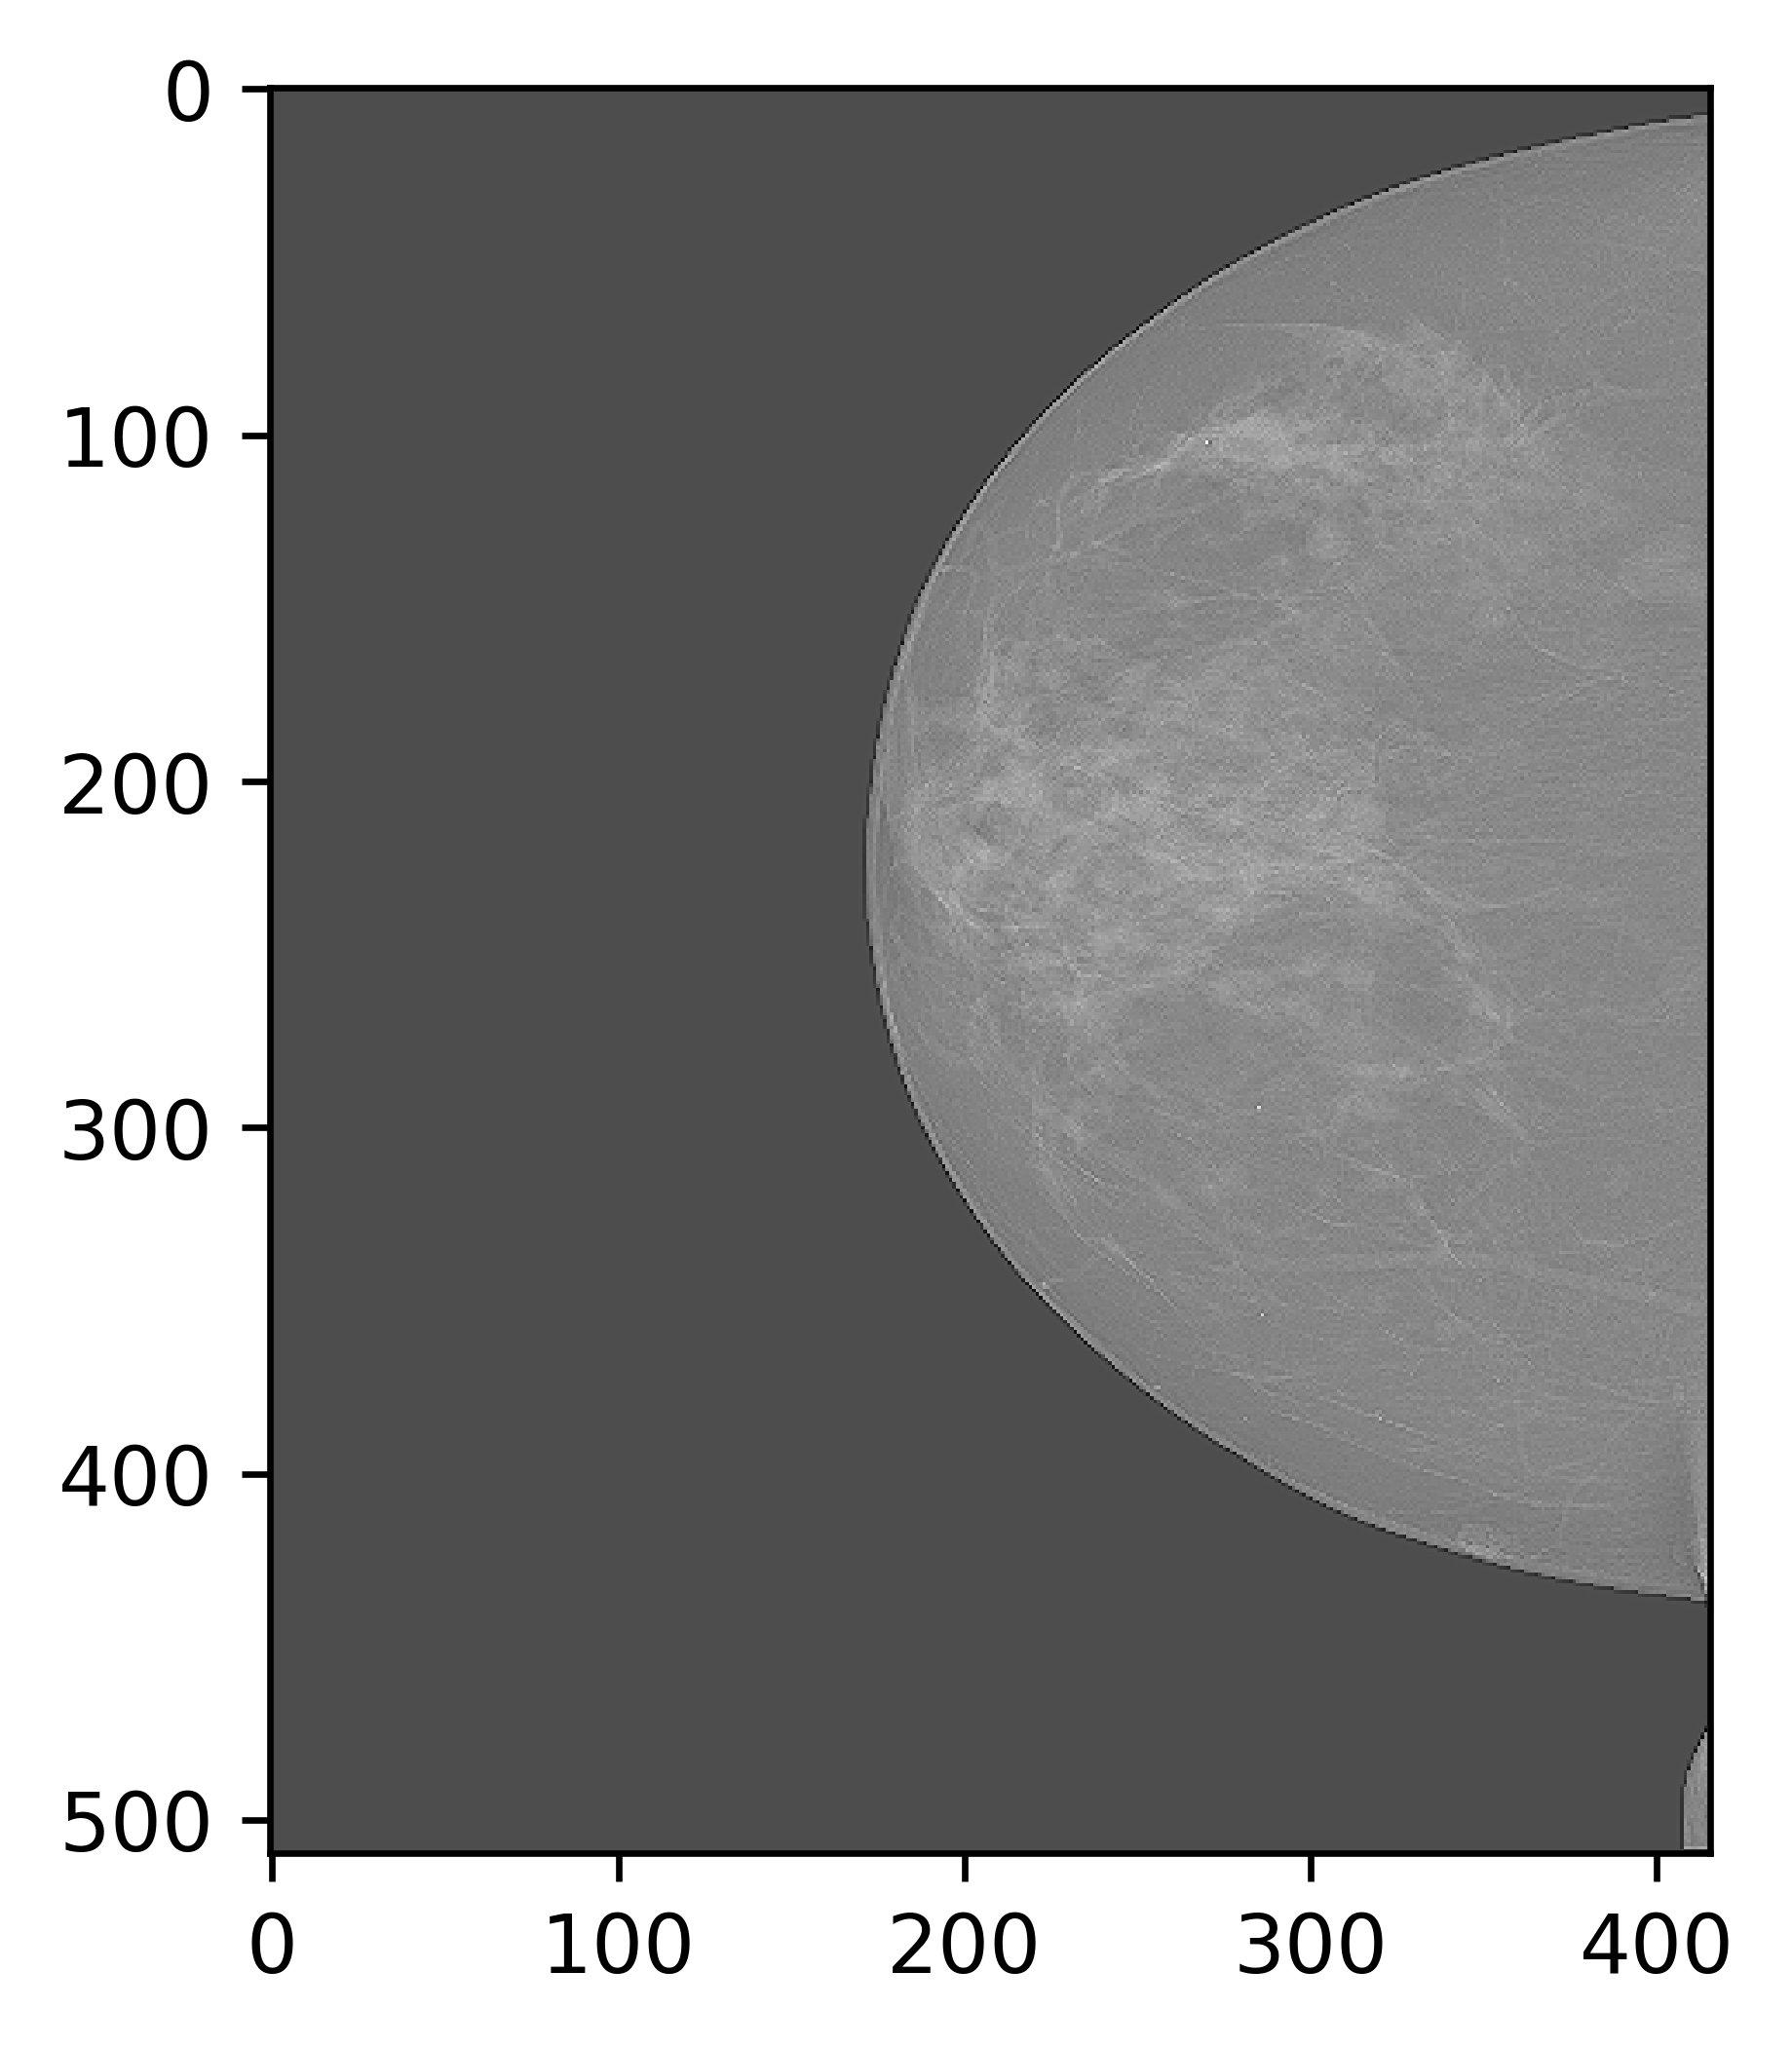
\includegraphics[scale=0.9]{Graphics/mm-fusion.png}}\par
	\end{multicols}
	\caption{Ejemplo de mamografía.} \label{fig:example-mm}
\end{figure*}


\begin{figure}
	\centering
	\subfigure[Masas]{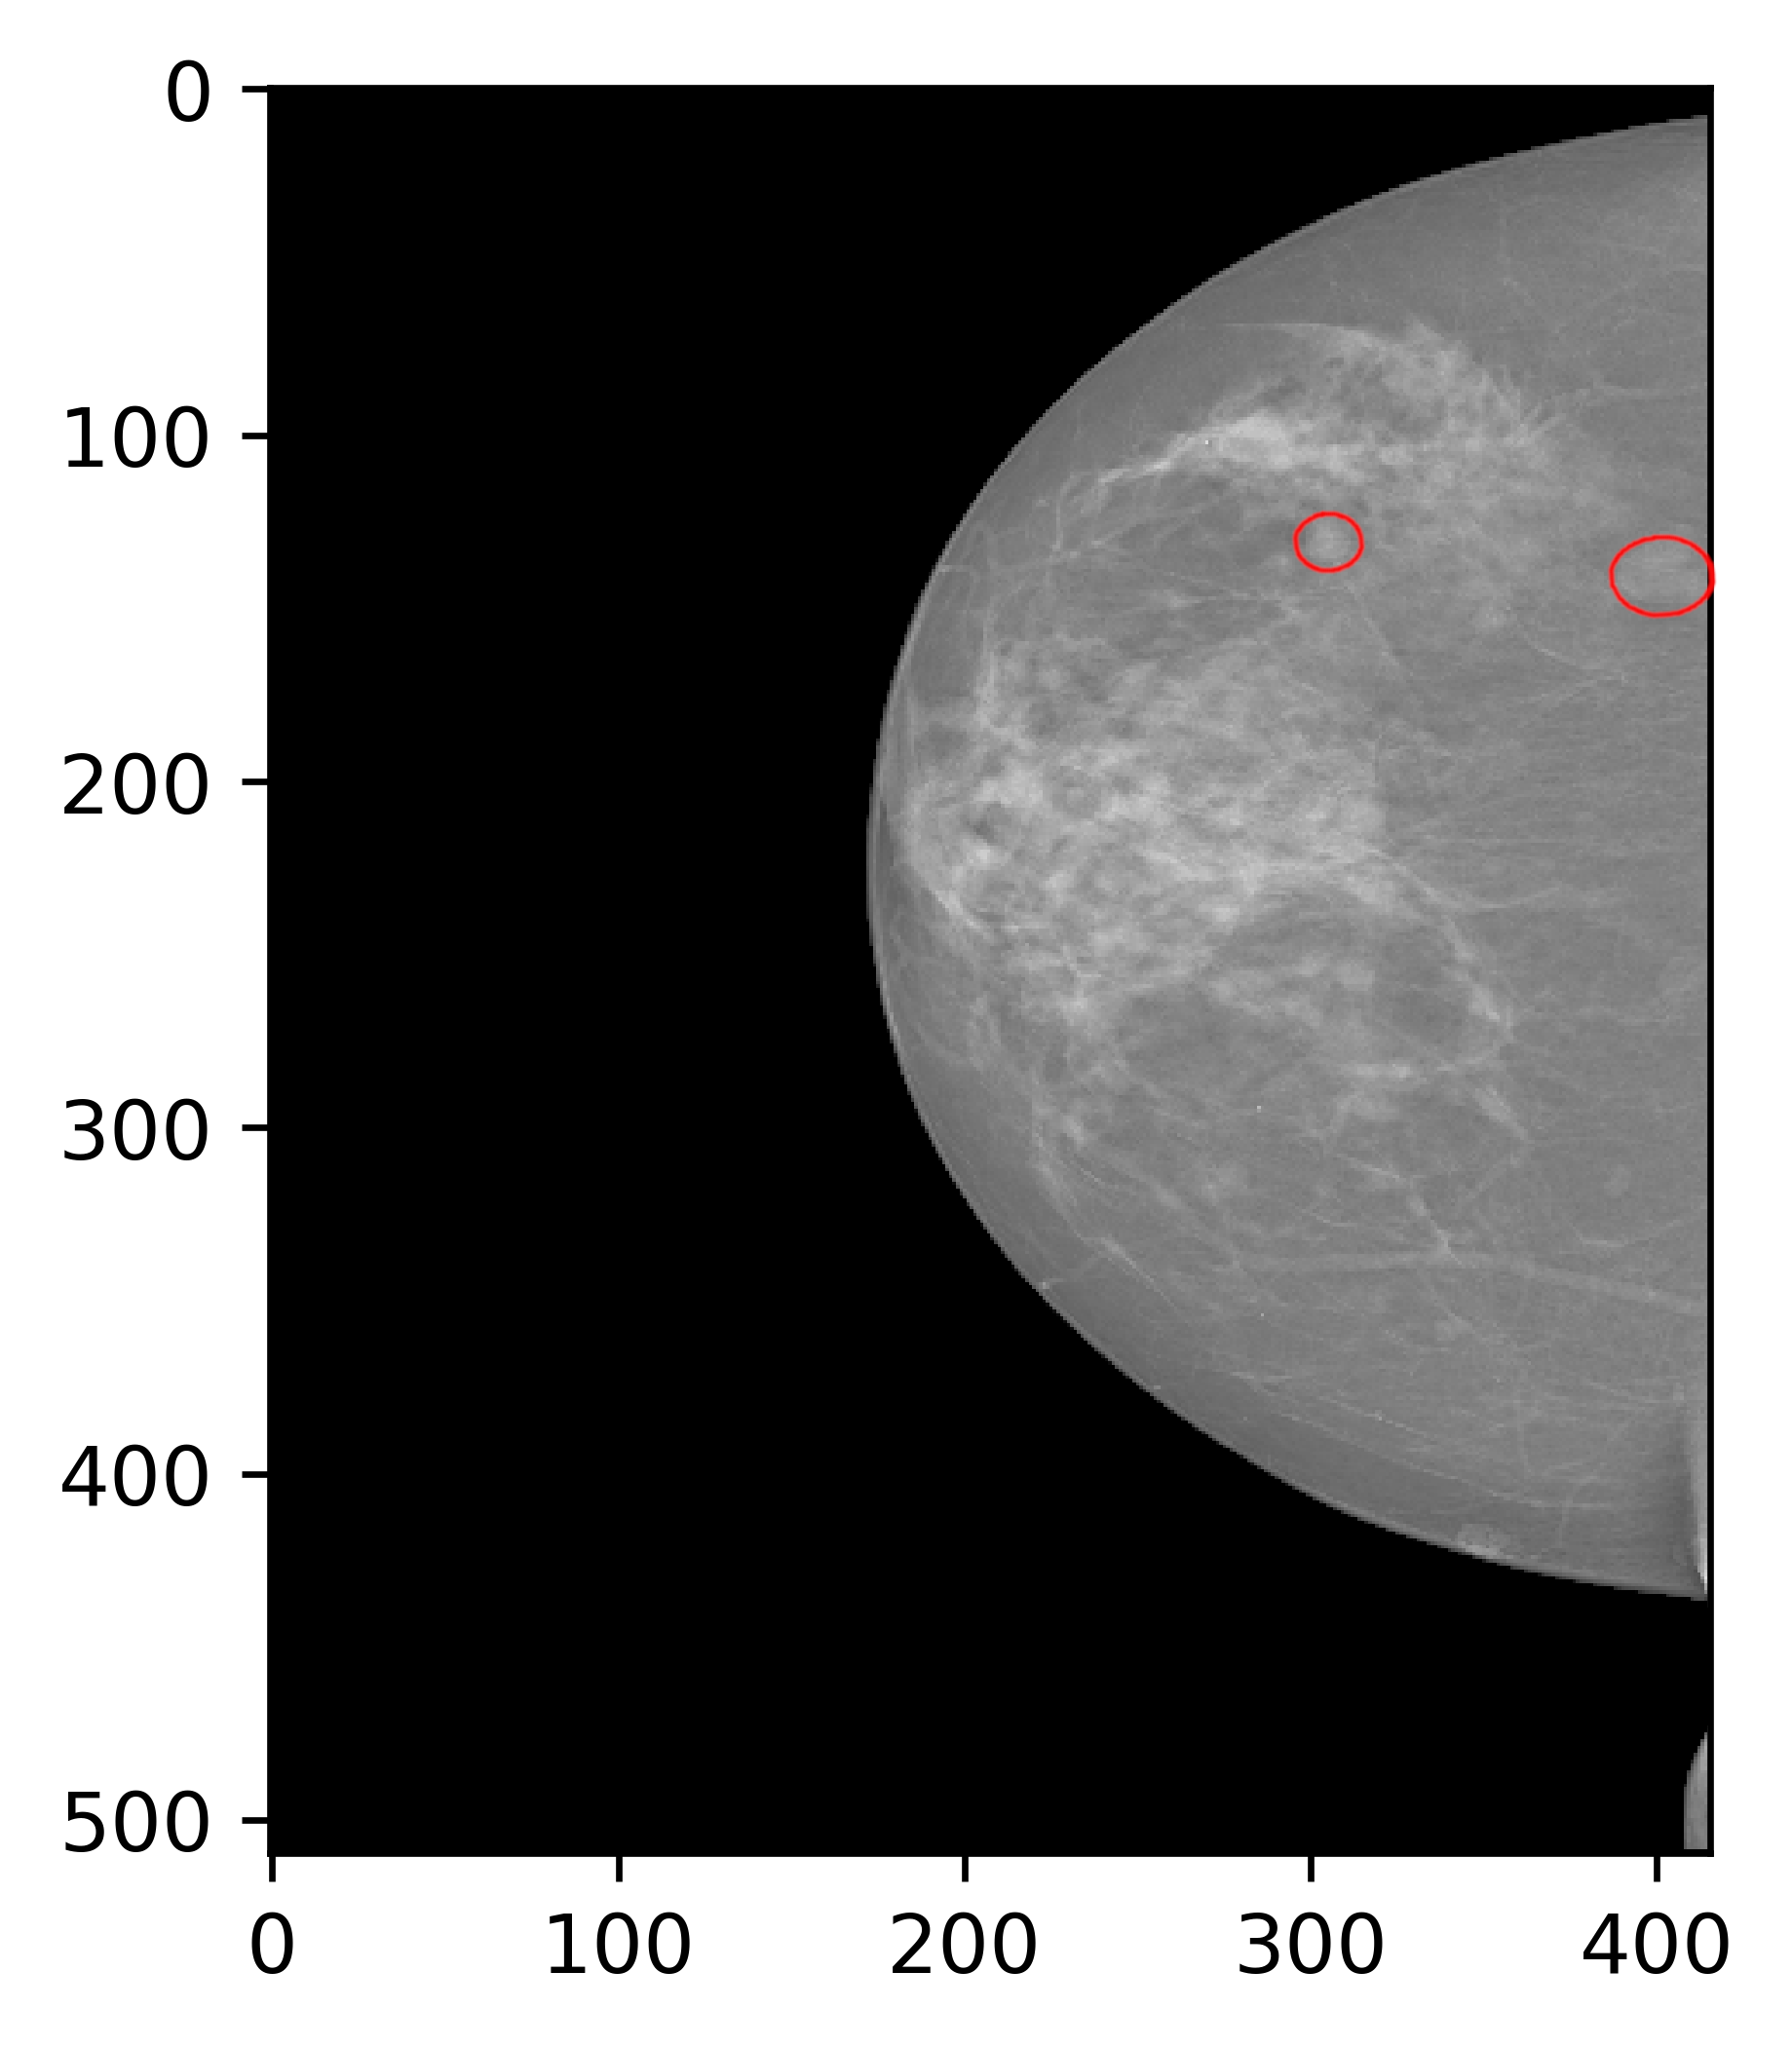
\includegraphics{Graphics/mm-rescaled-mass.png}}
	\subfigure[Porción de la mamografía donde se aplica el algoritmo]{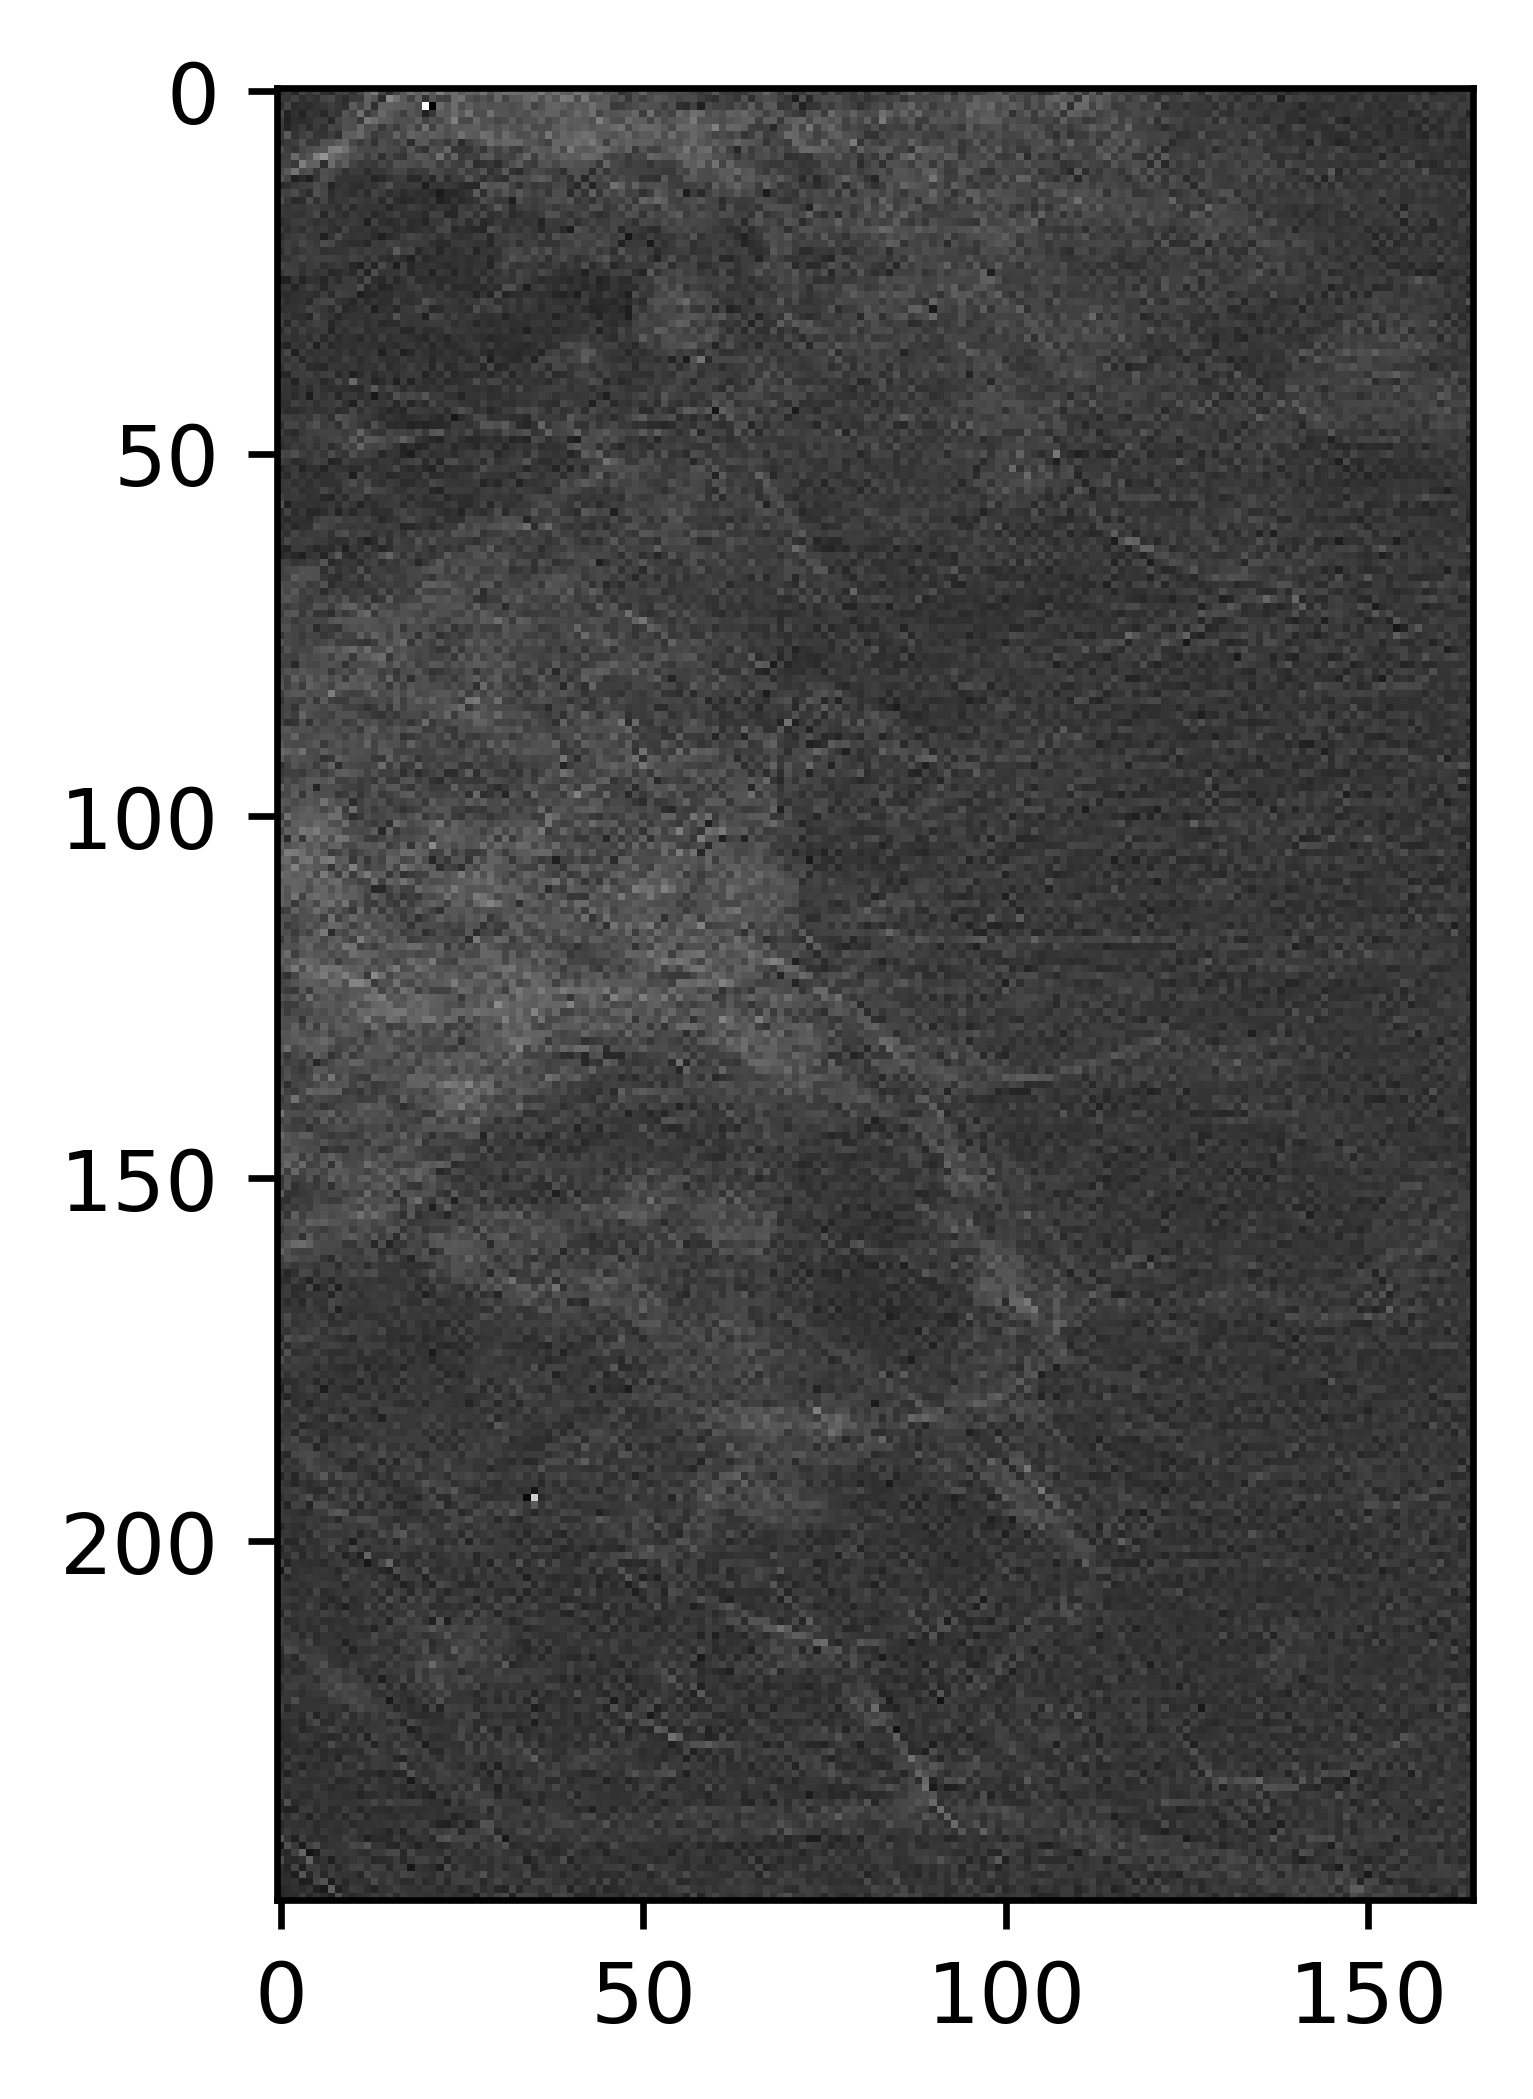
\includegraphics{Graphics/mm-portion.png}}
	\caption{Mamografía con la ubicacioón de las masas y la sección donde se aplica el algoritmo.} \label{fig:example-mm-portion}
\end{figure}

En la imagen de ejemplo existen dos masas. Pero solo se toma una para construir la(s) shapelet(s), de este modo 
se evalúa la capacidad del algoritmo para la detección de masas en general. En el caso ideal debería detectar ambas
regiones. Otro aspecto importante es que para el experimento se toma una sección de la mamografía donde no aparece 
el fondo negro, debido a que introduce muchos falsos positivos por el hecho de que los píxeles sean iguales a
cero. 

La Figura \ref{fig:example-mm-portion} muestra la ubicación de las masas y la porción de la mamografía sobre
la cual se realiza el algoritmo de detección. La primera de izquierda a derecha es la seleccionada para construir
la(s) shapelet(s).

\begin{figure*}
	\begin{center}
	\begin{multicols}{2}
		\subfigure[Coeficientes de aproximación]{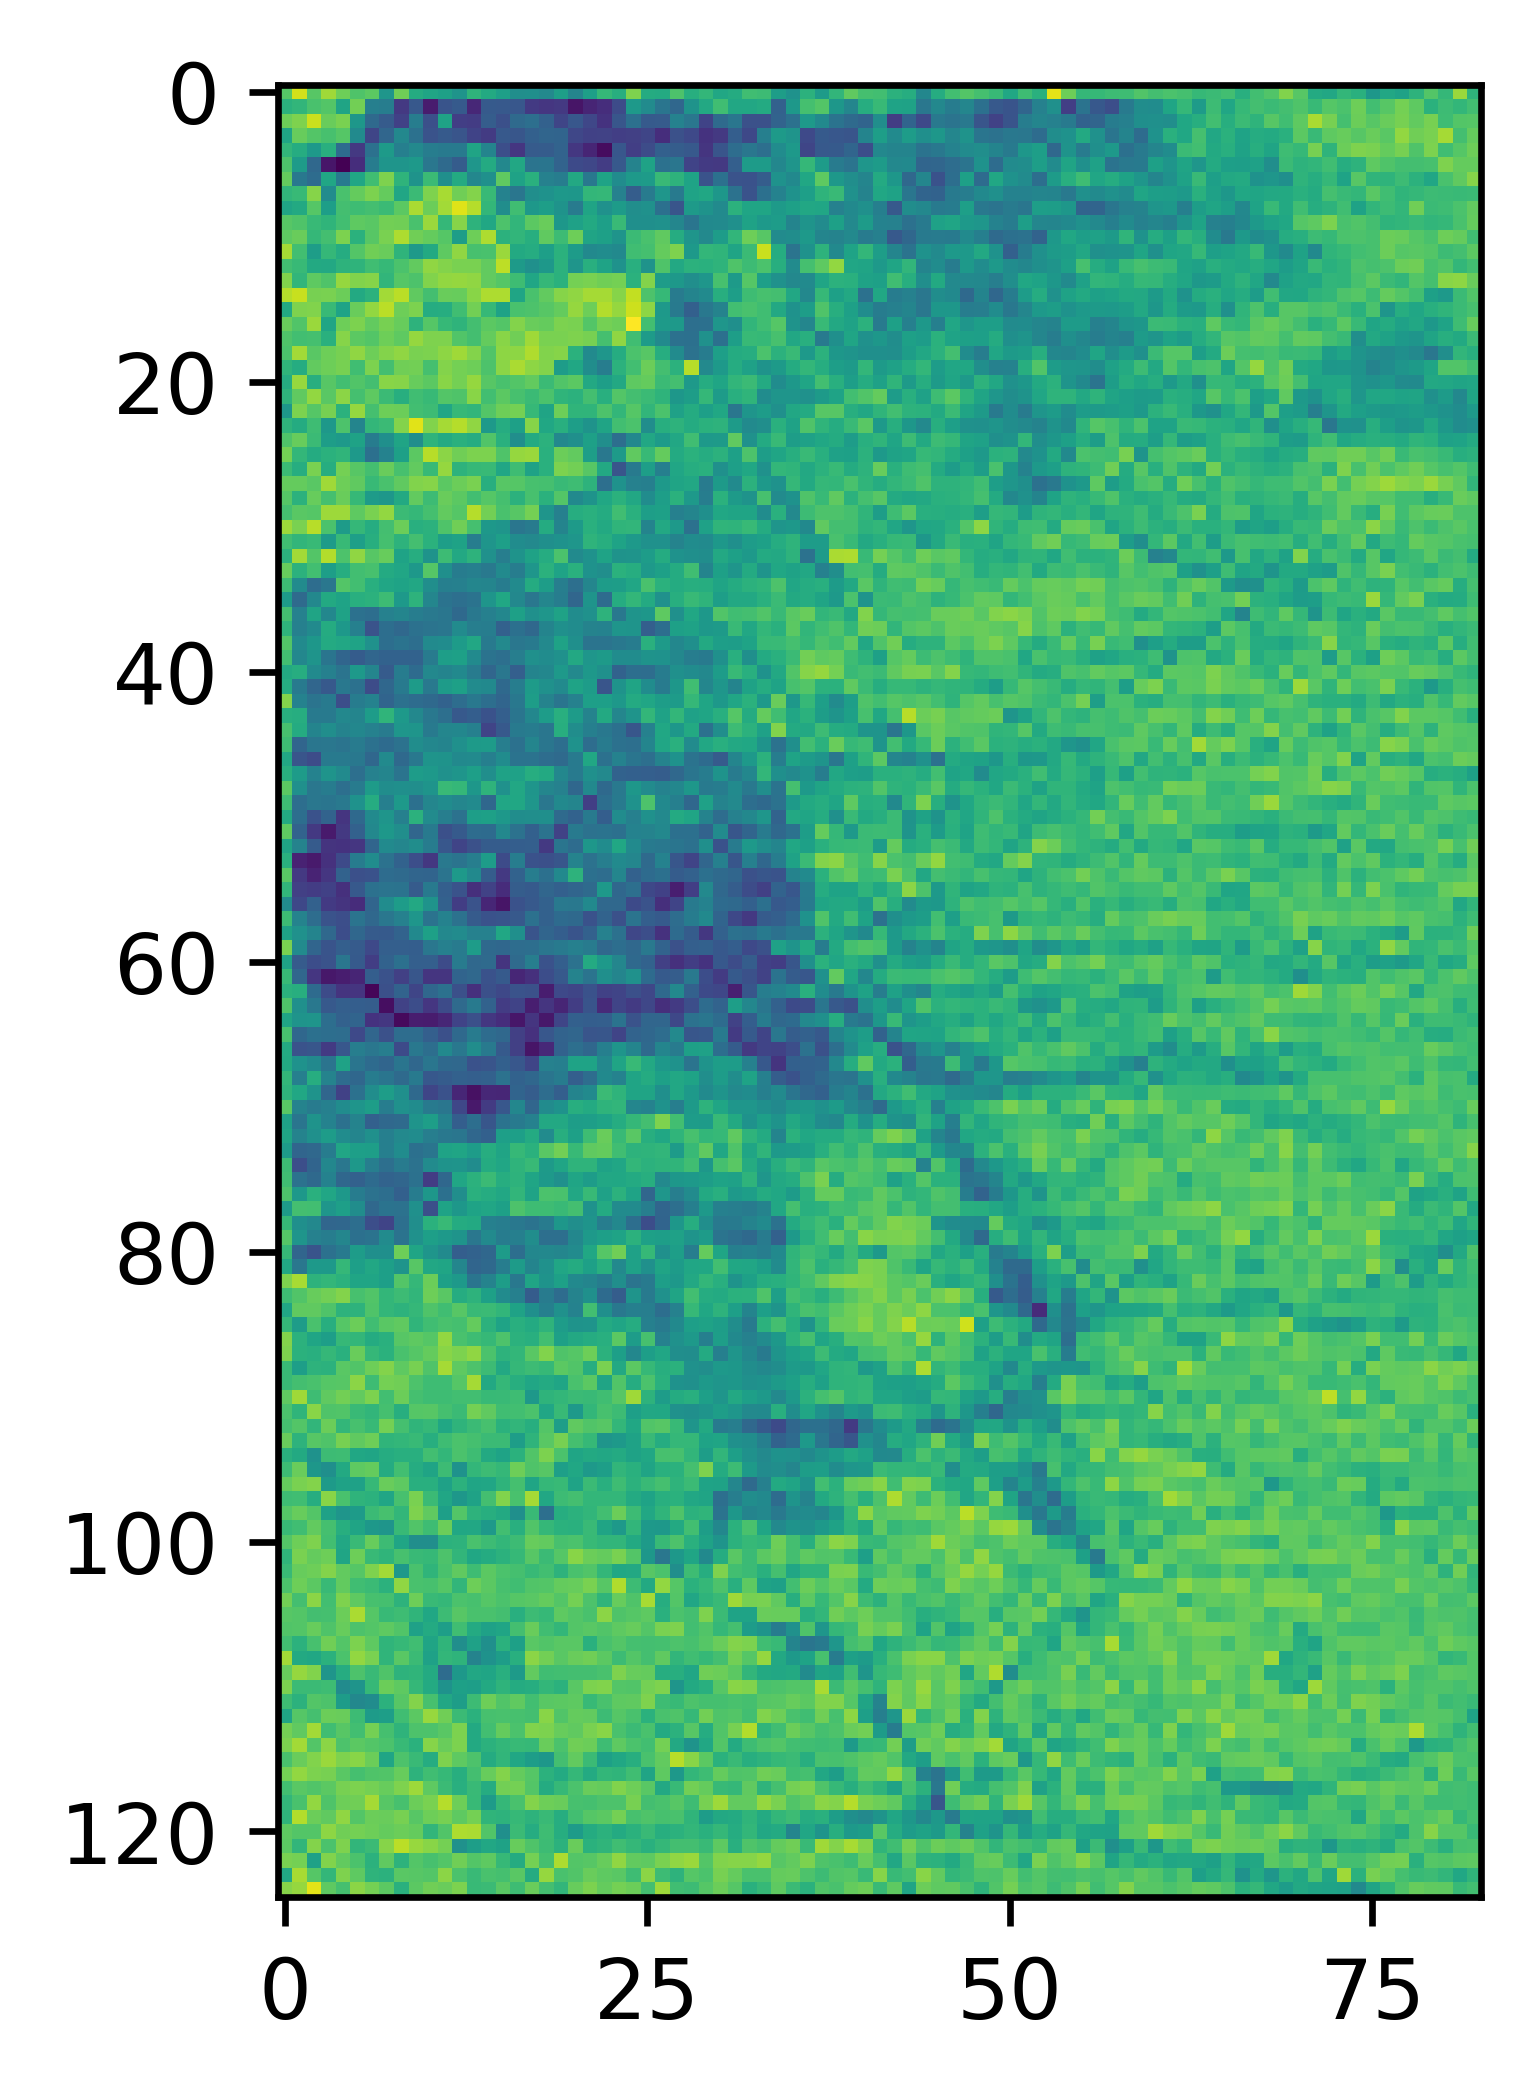
\includegraphics[scale=0.95]{Graphics/mm-aprox.png}}
		\subfigure[Coeficientes de detalle horizontal]{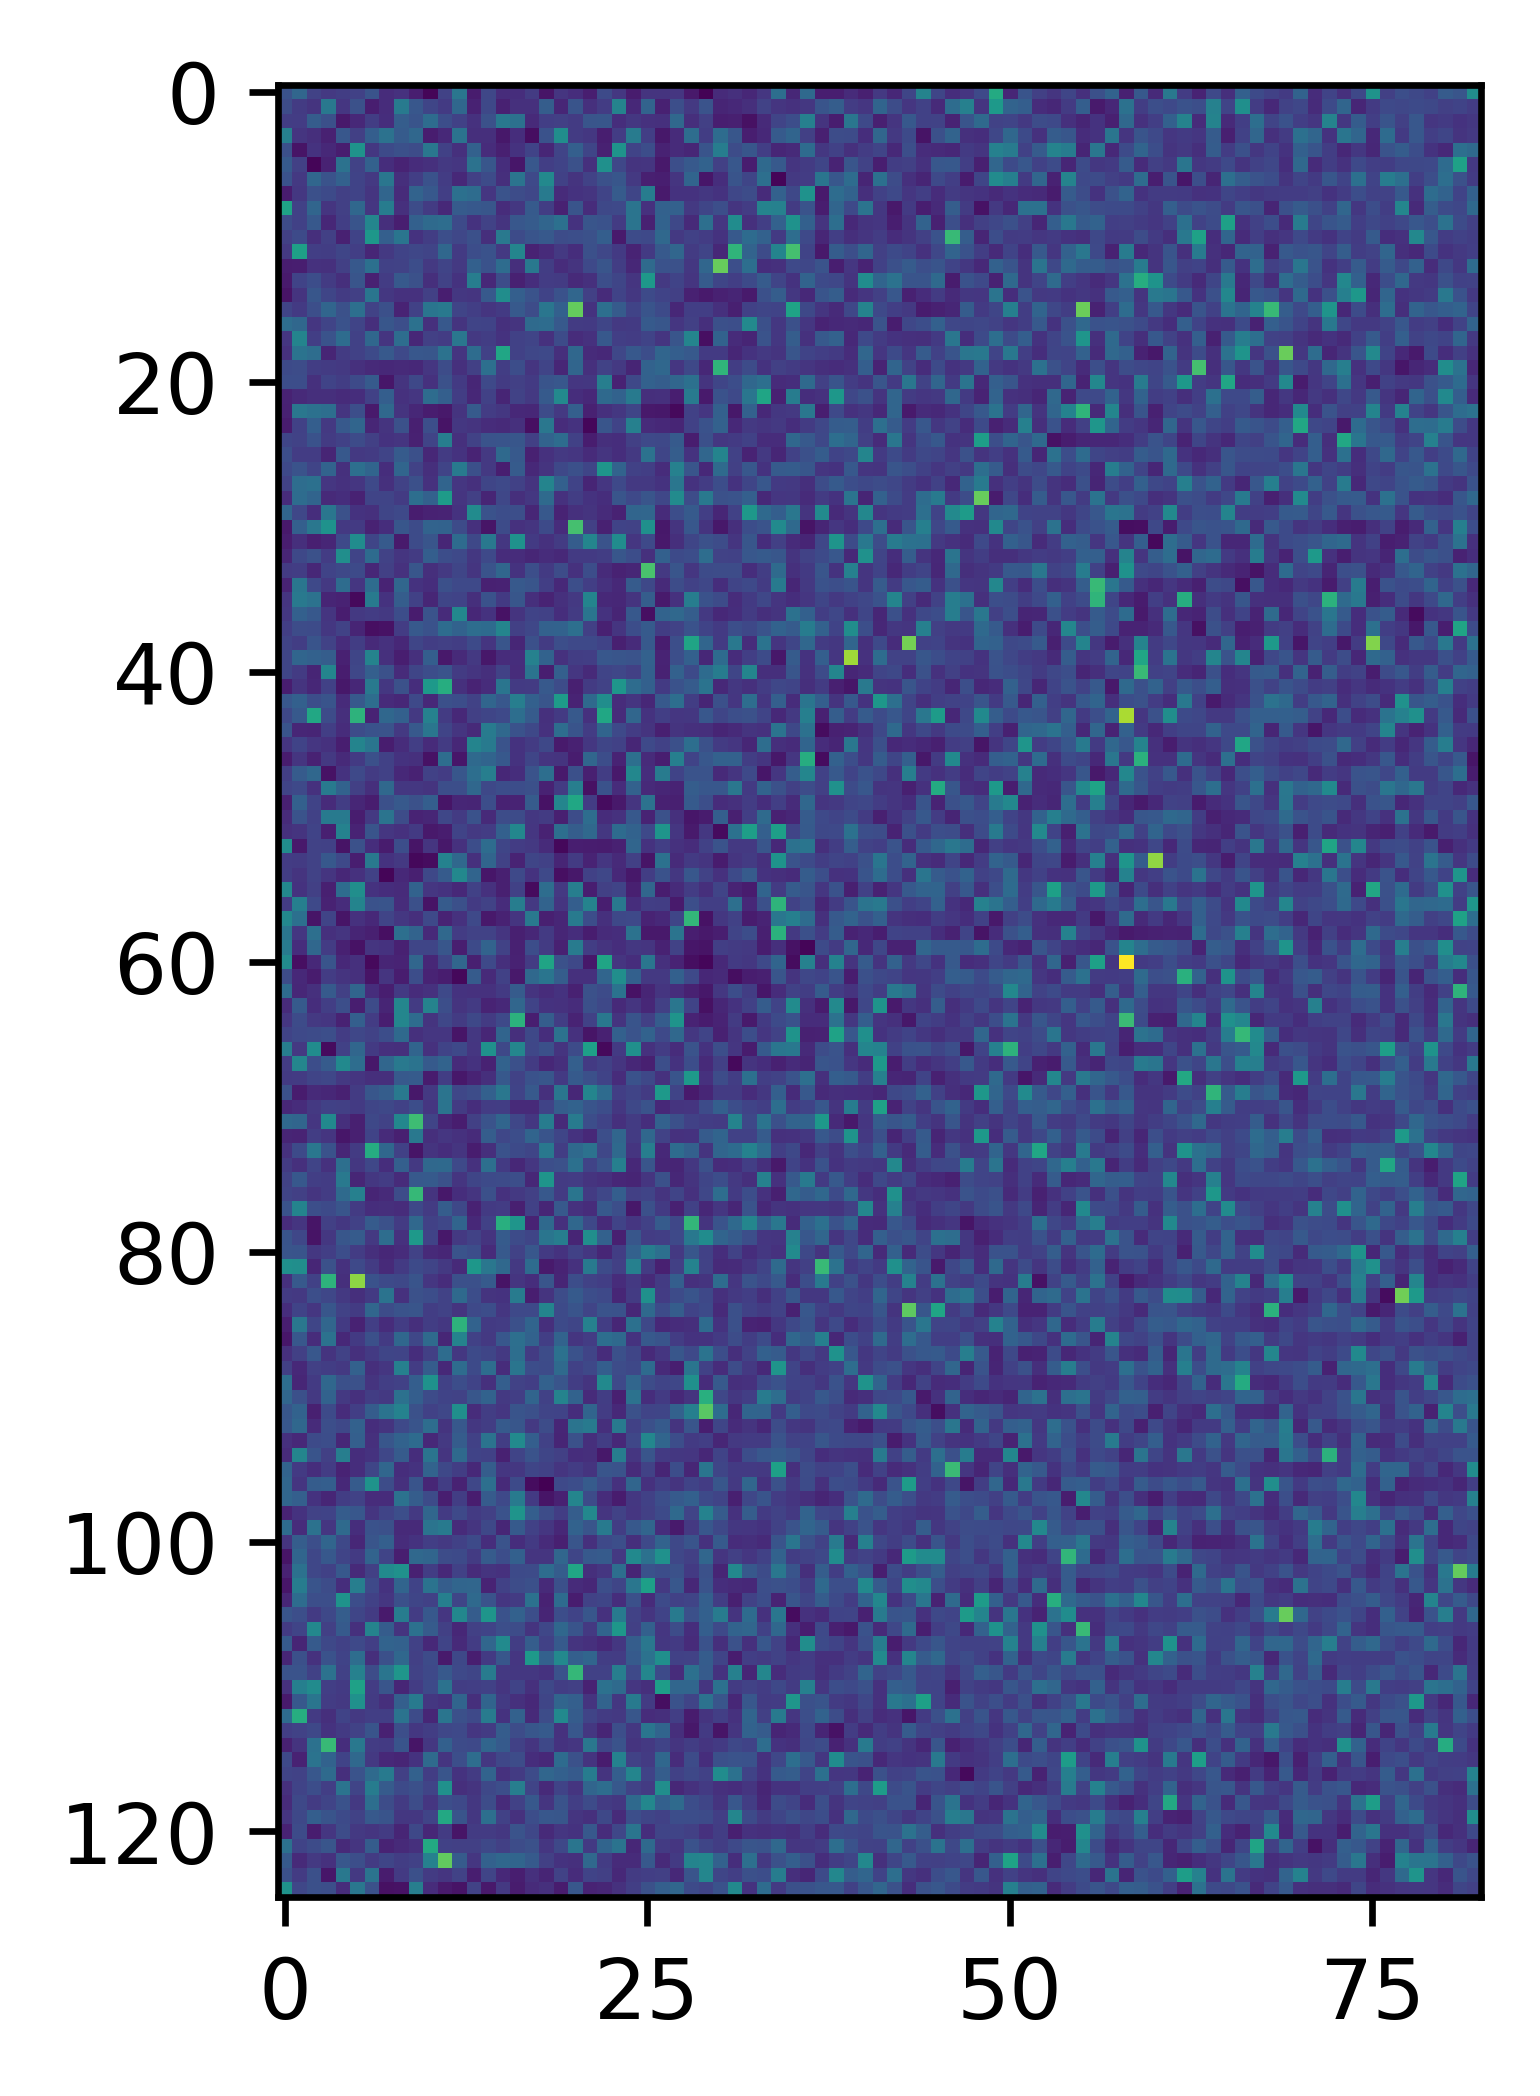
\includegraphics[scale=0.95]{Graphics/mm-horizontal.png}}
    \end{multicols}
	\begin{multicols}{2}
		\subfigure[Coeficientes de detalle vertical]{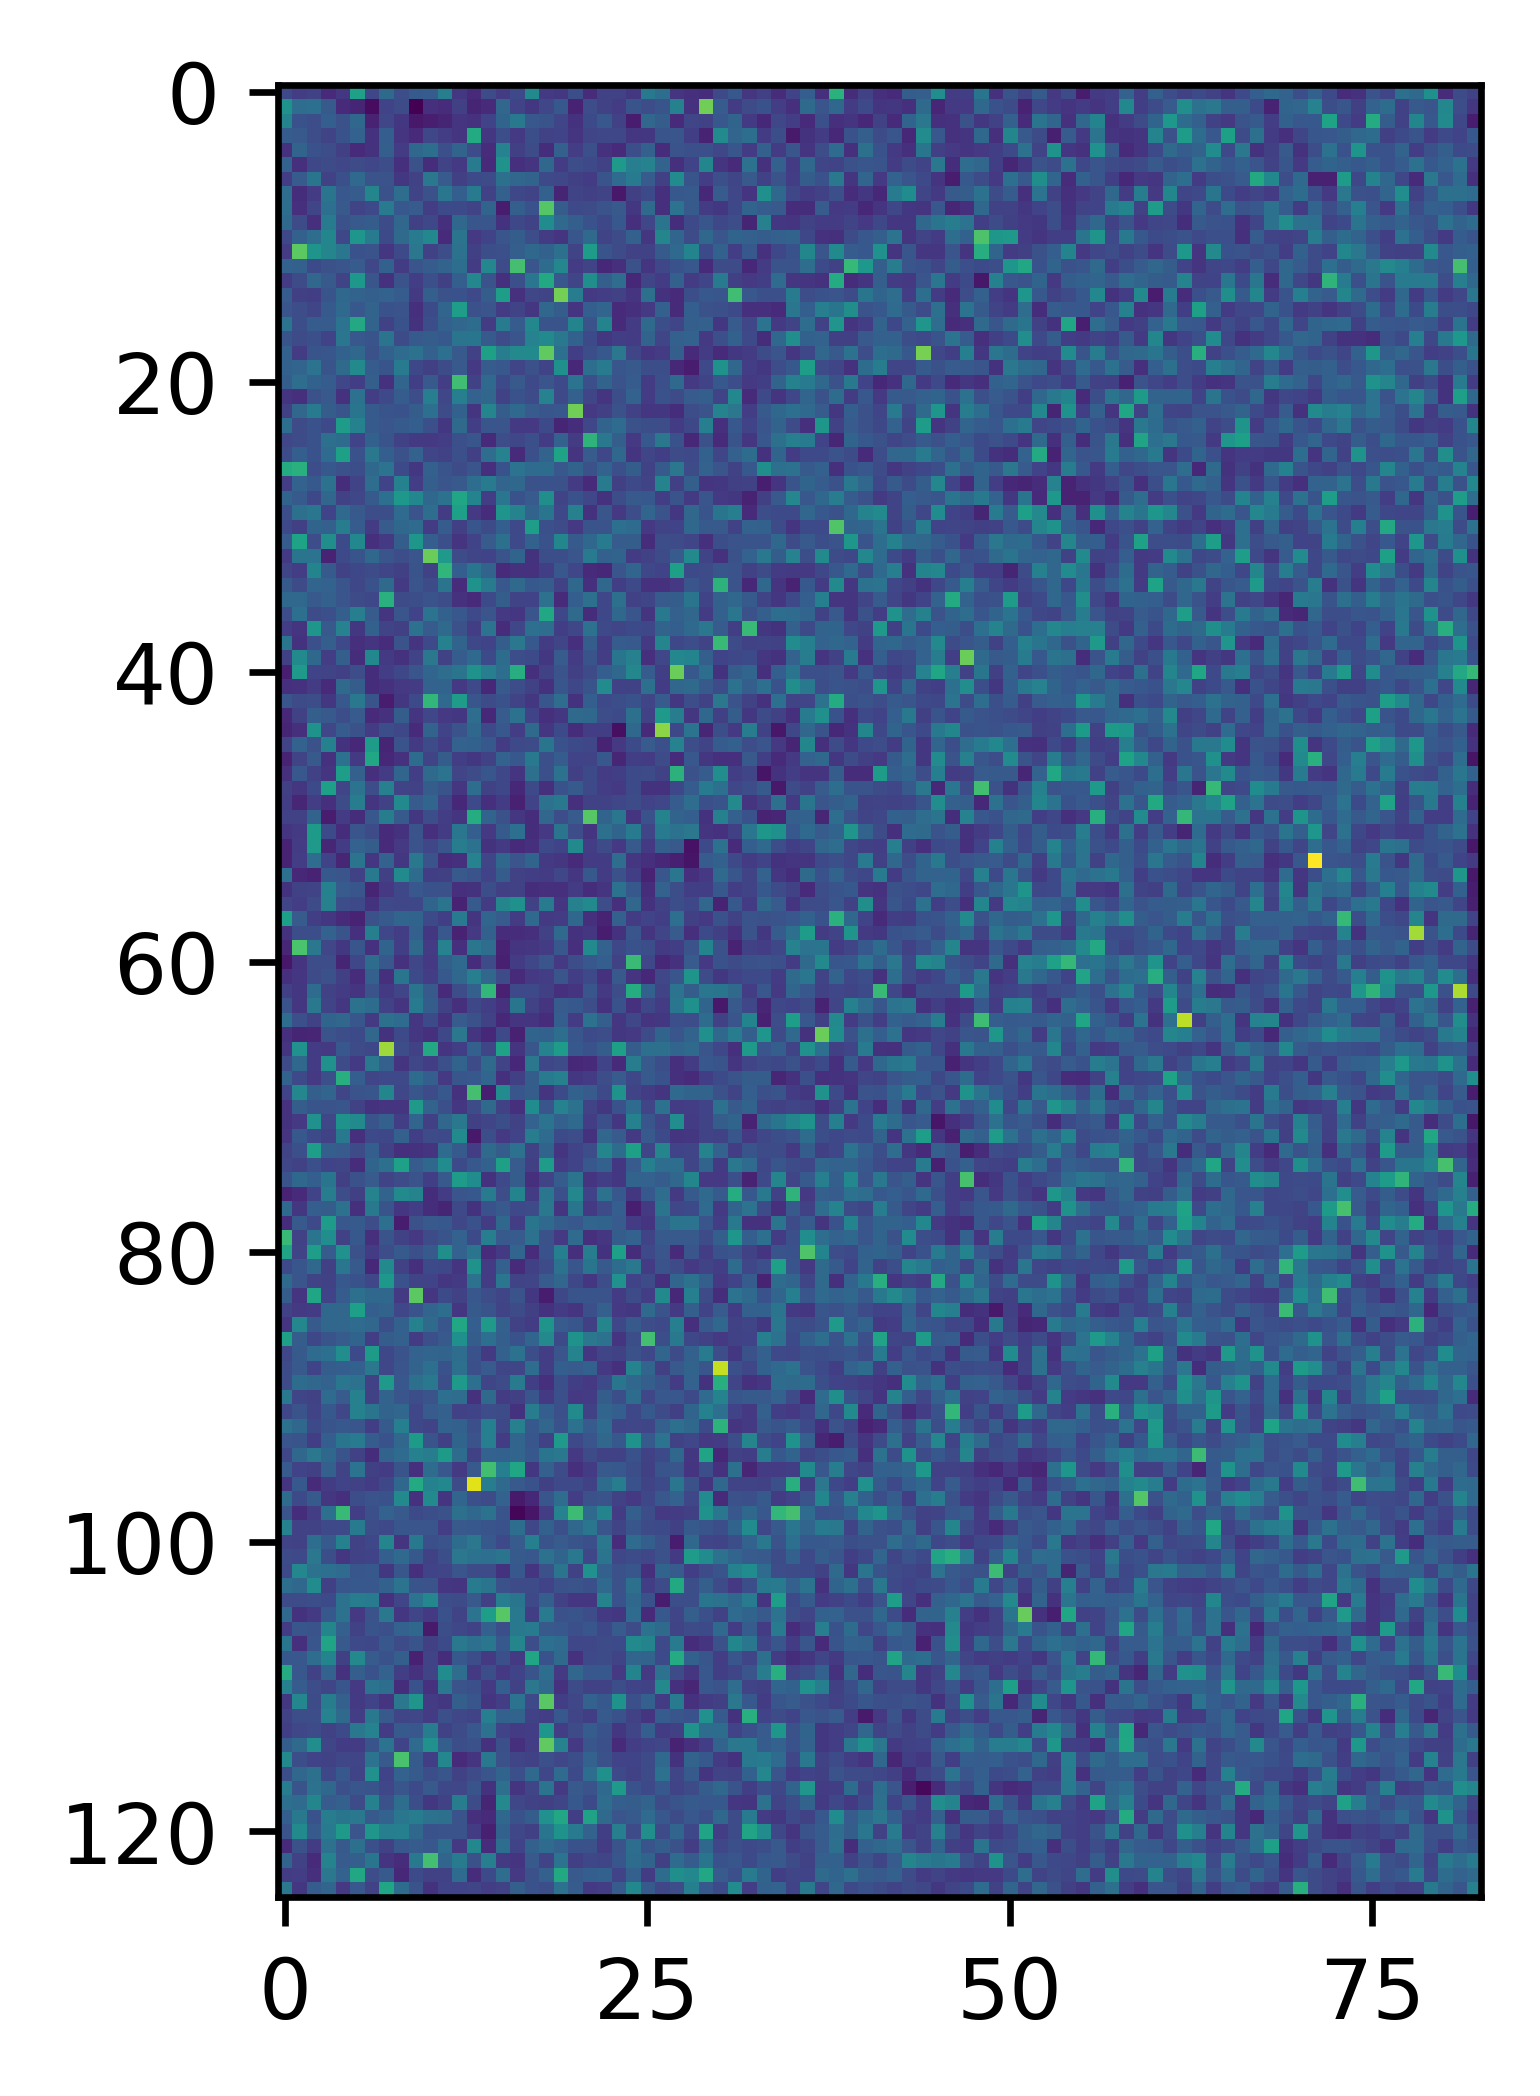
\includegraphics[scale=0.95]{Graphics/mm-vertical.png}}
		\subfigure[Coeficientes de detalle diagonal]{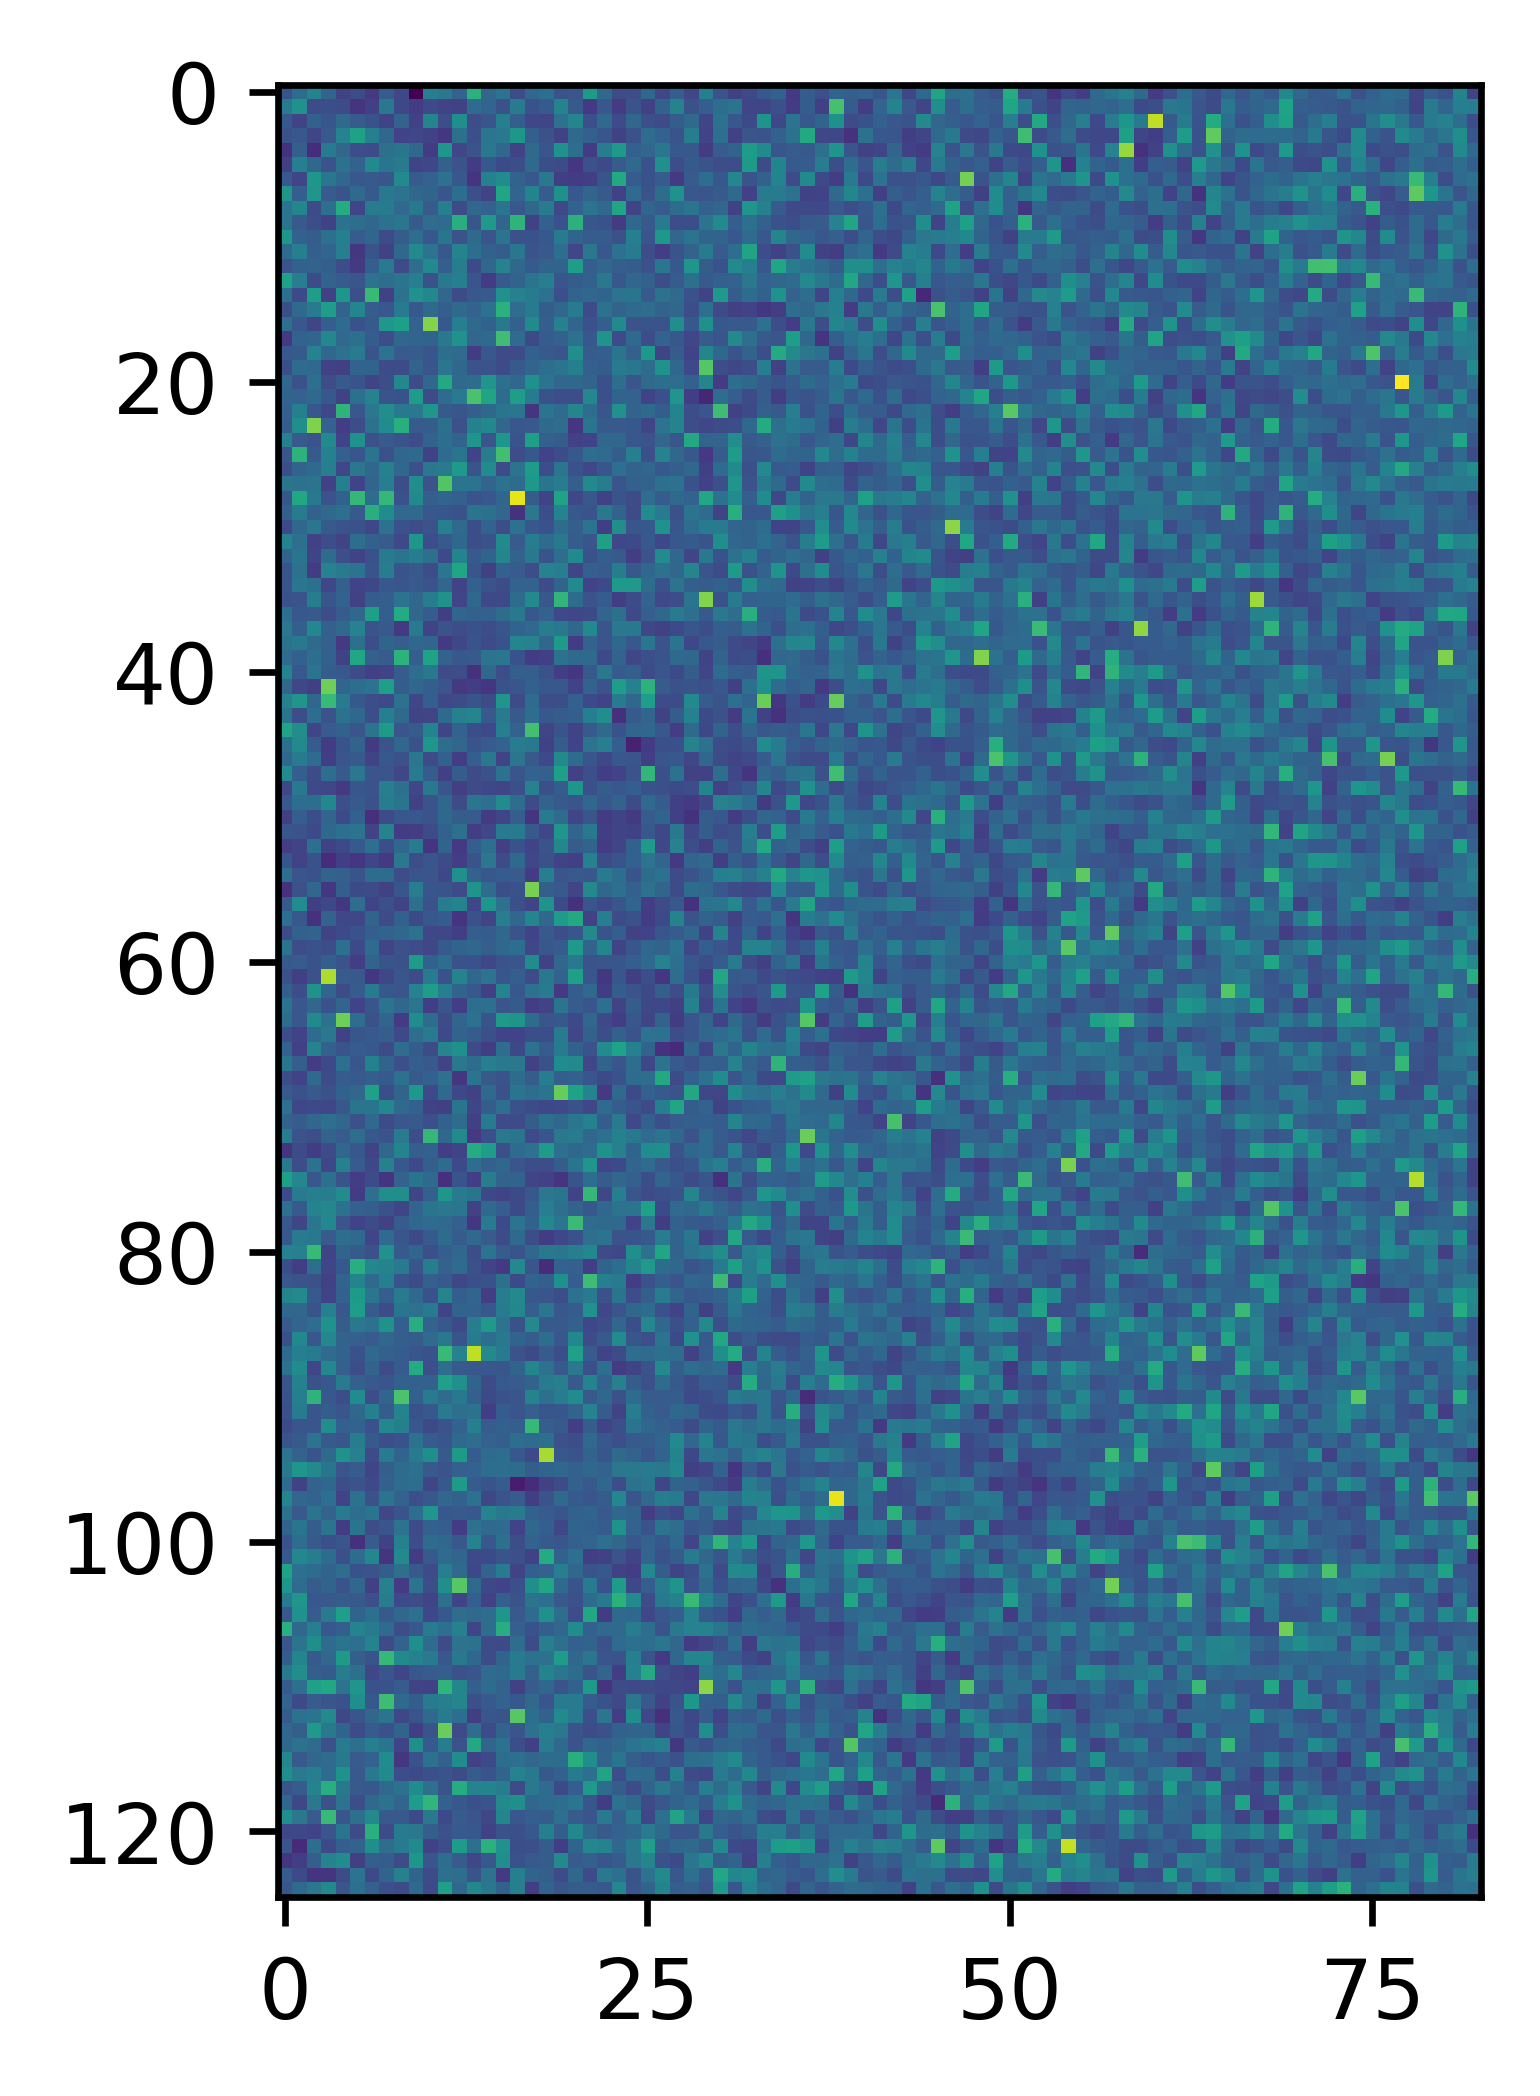
\includegraphics[scale=0.95]{Graphics/mm-diagonal.png}}
	\end{multicols}
	\end{center}
\caption{Resultado de la medida $\mathbb{S}$ sobre cada una de las cuatro componentes de la DST-II.} \label{fig:example-mm-approach1}
\end{figure*}

El resultado del primer enfoque se muestra en la Figura \ref{fig:example-mm-approach1}. Nótese que
tanto en este caso como en el
del ejemplo de la gaussiana, no hay ningún signo de detección. Esto refuerza aún más la conclusión de que la DST-II no se puede
extender para el caso 2D con este enfoque.

\begin{figure}
	\centering
	\subfigure[Por filas]{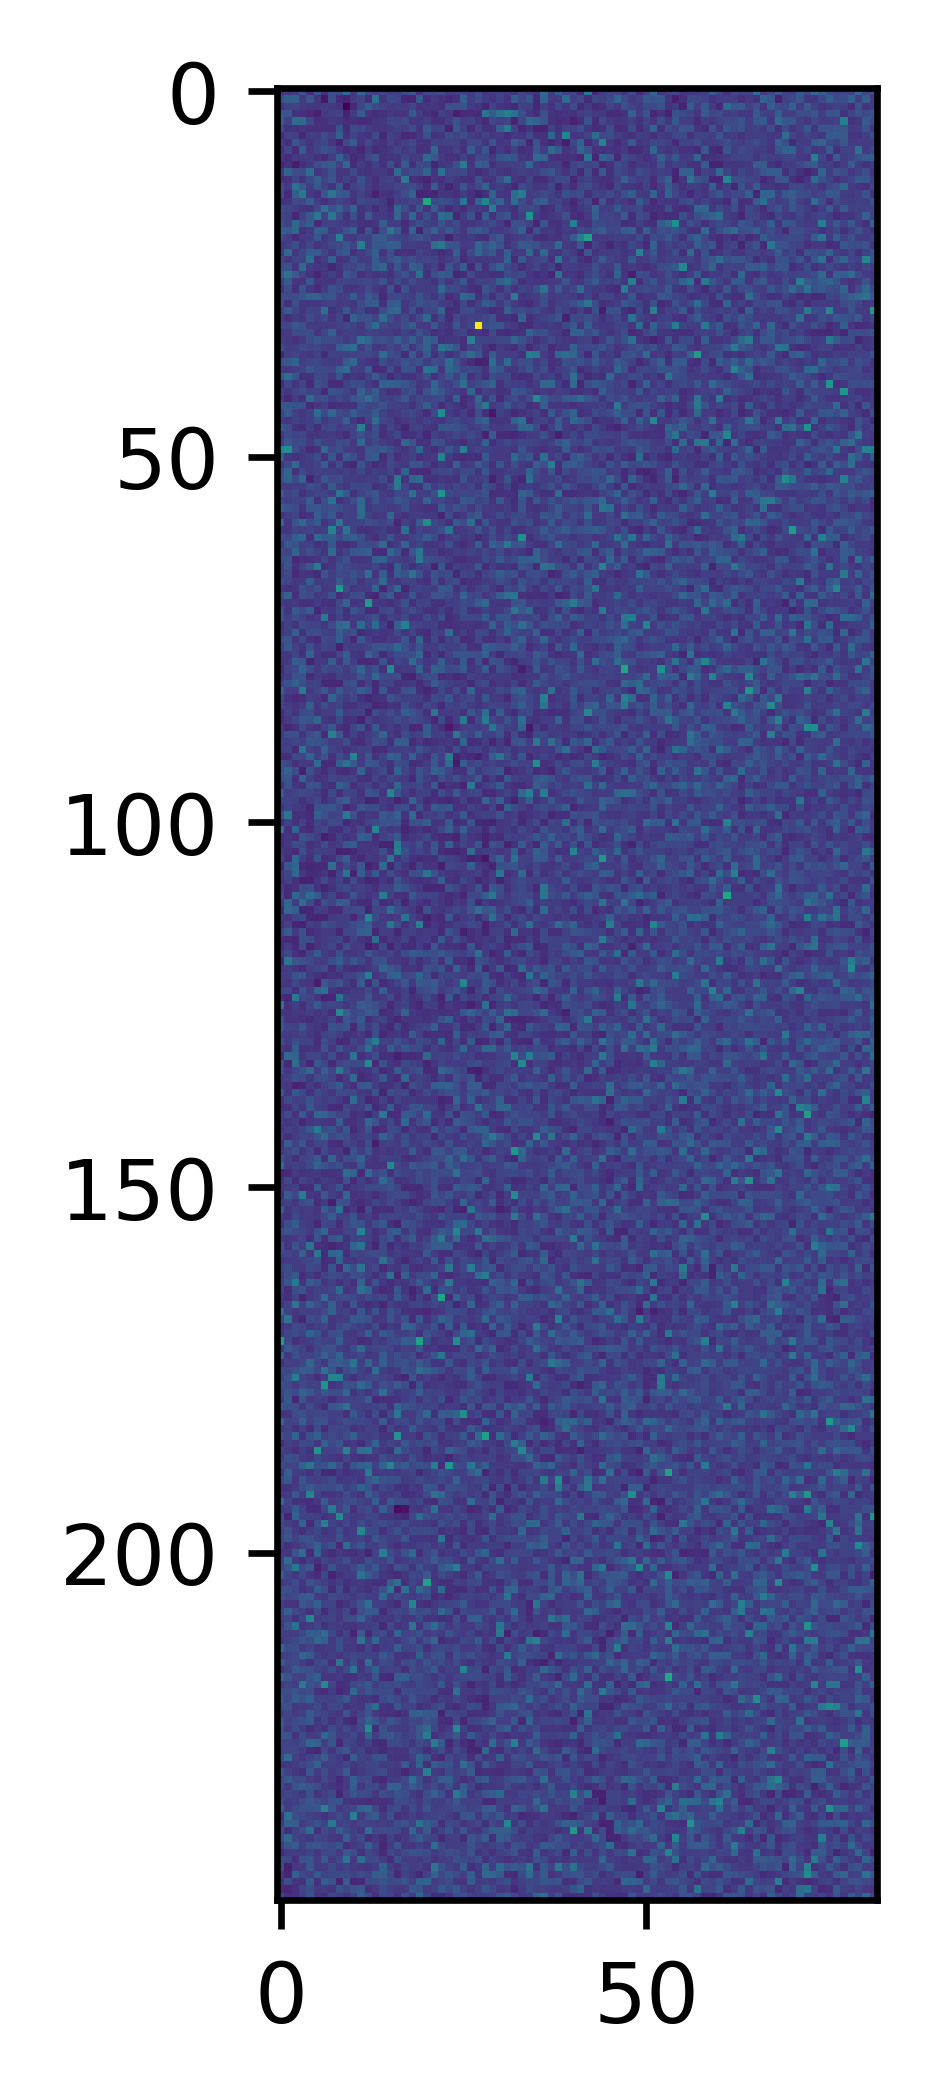
\includegraphics{Graphics/mm-row.png}}
	\subfigure[Por columnas]{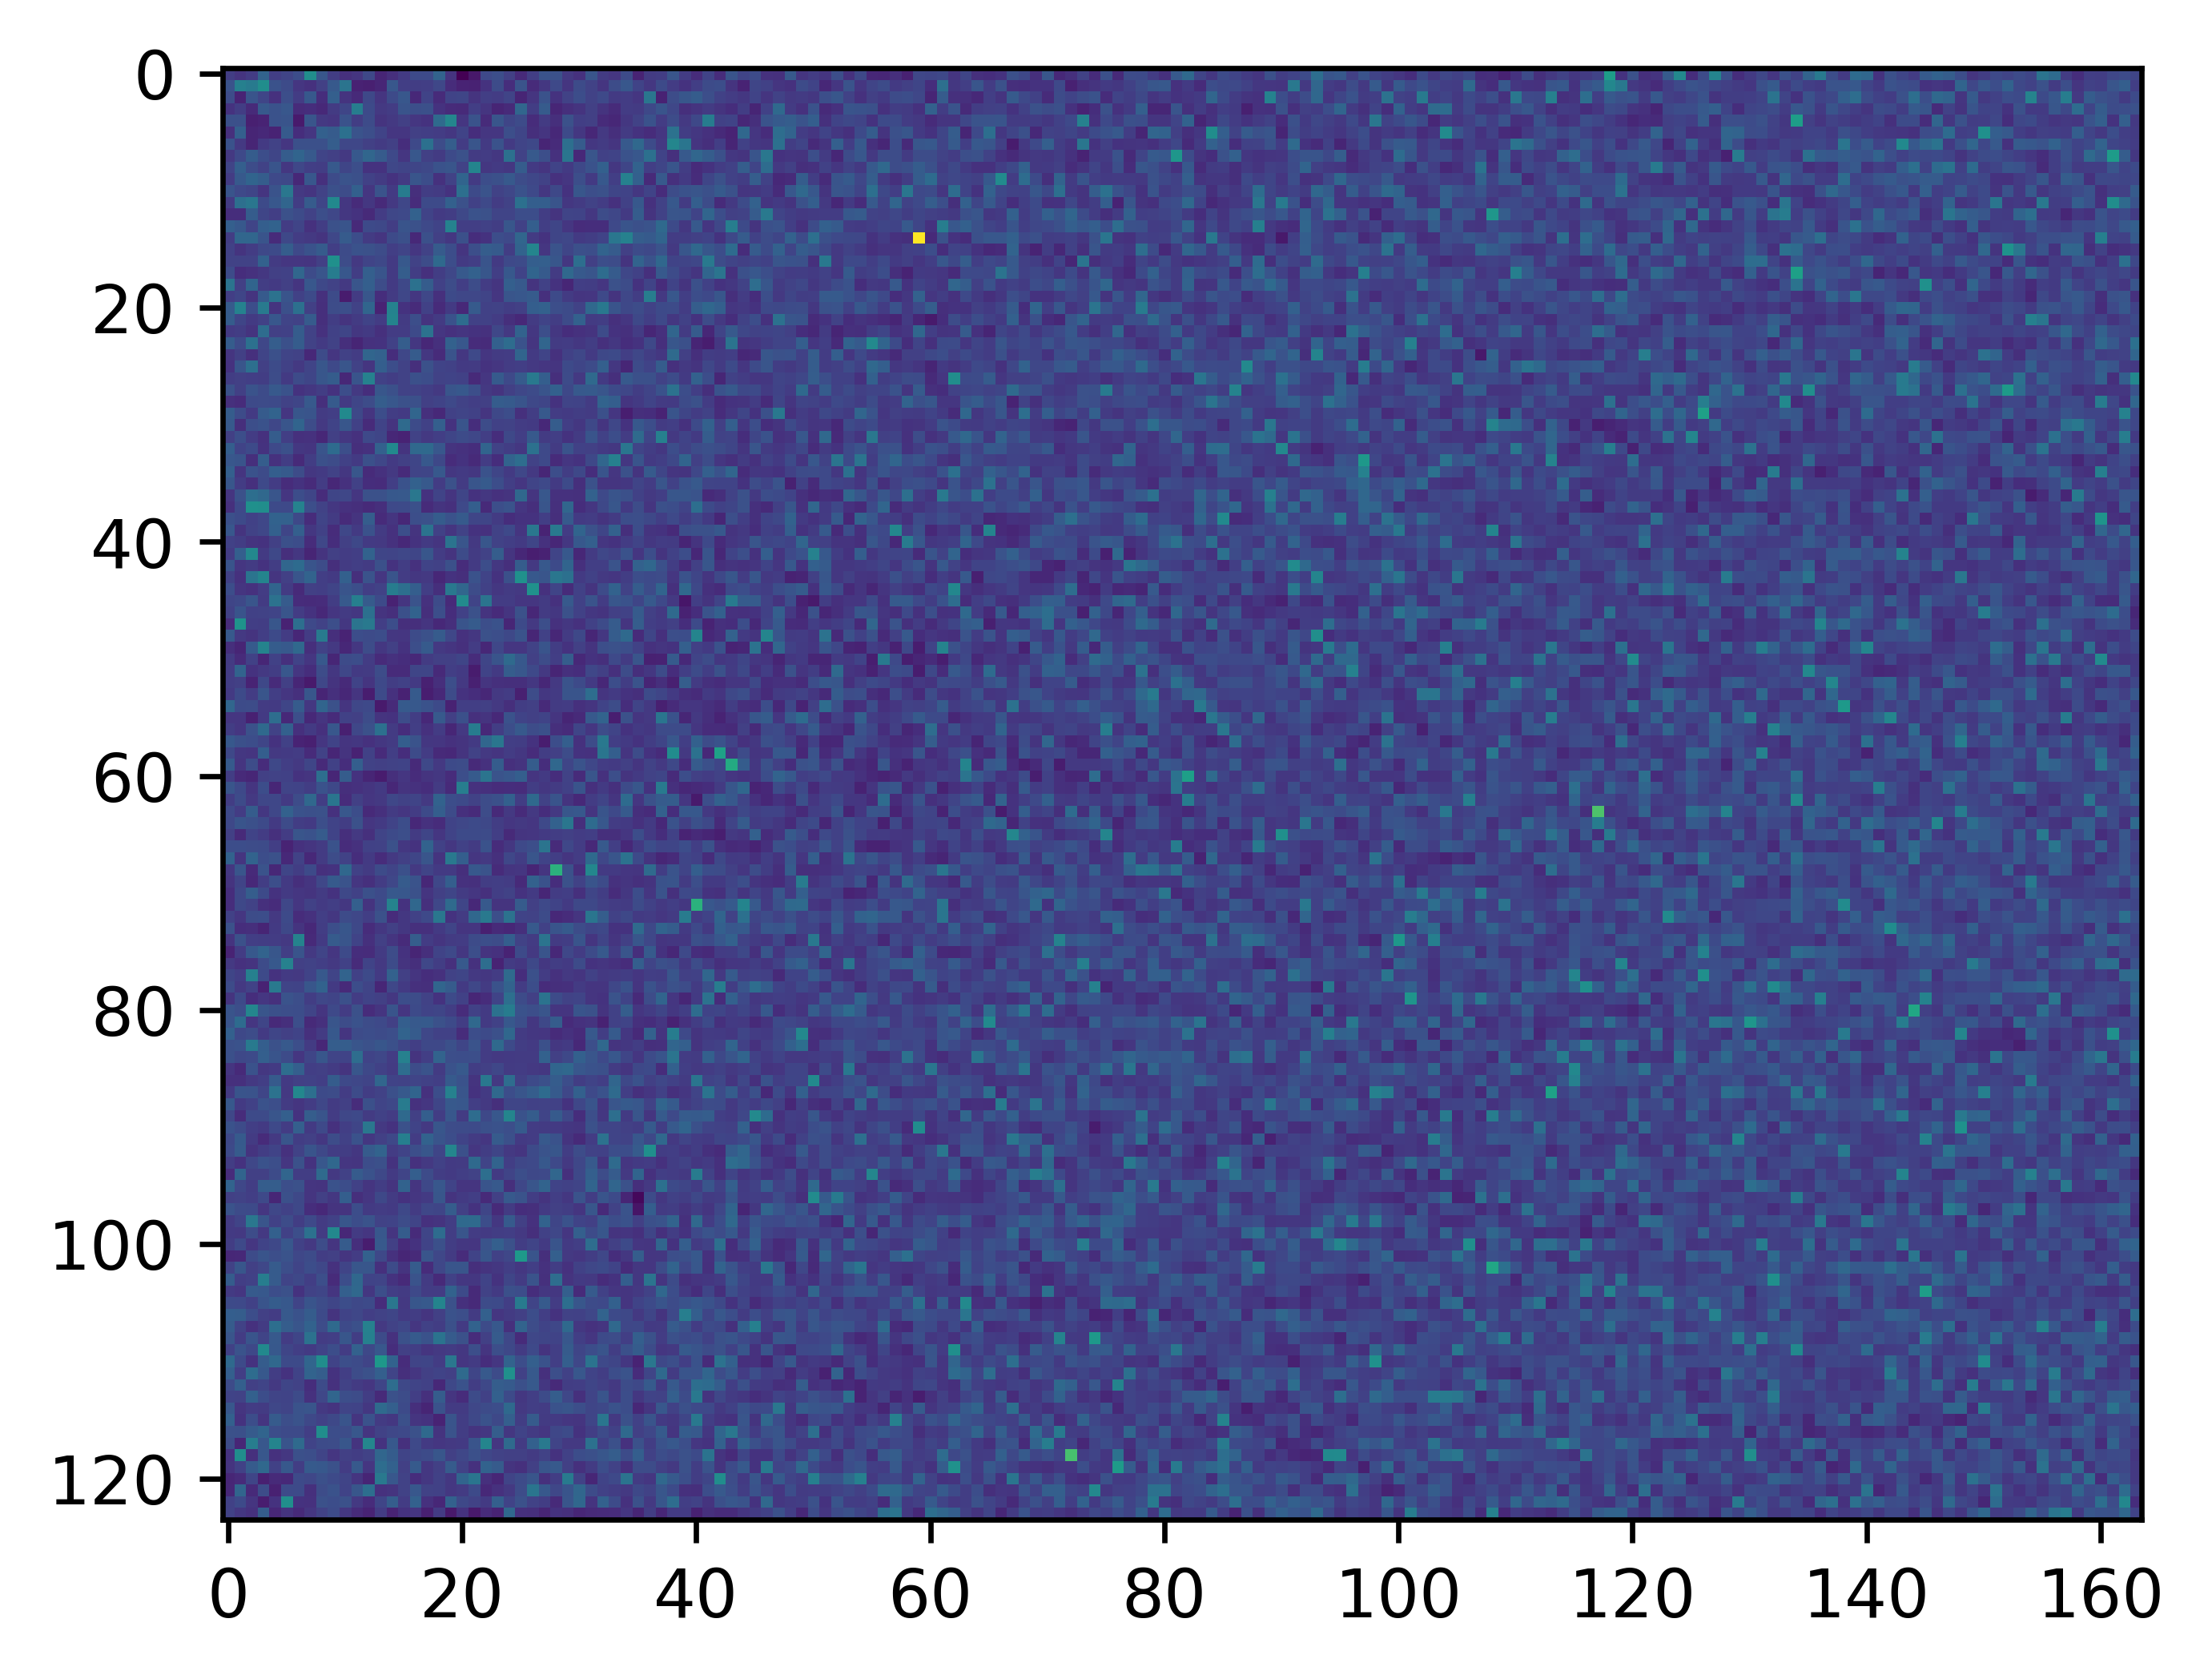
\includegraphics{Graphics/mm-col.png}}
	\caption{Resultado de evaluar $\mathbb{S}$ sobre cada una de las \textit{second-rated} de la DST-II usando el segundo enfoque.} \label{fig:example-mm-approach2}
\end{figure}
%Detection at position (32, 27) with value 0.9831863519468129 row
%Detection at position (14, 59) with value 0.983604207430764 col

En el caso del segundo enfoque, los resultados son mejores. Si se observa la Figura \ref{fig:example-mm-approach2}, al menos hay signos de detección.
Aunque bien difíciles de ver, existen un par de píxeles (de color amarillo), uno en cada imagen que constrastan con el resto.
Estos están ubicados en las posiciones $(32,27)$ y $(14,59)$ con valores $0.9831863519468129$ y $0.983604207430764$,
respectivamente. Ambos corresponden a las posiciones aproximadas $(32,54)$ y $(28,59)$, que es donde se encuentra el patrón extraído.
La Figura \ref{fig:example-mm-approach3} muestra la mamografía con las posiciones 
predichas por el algoritmo basado en $\mathbb{S}$. Los píxeles de color rojo indican estas posiciones.
A pesar de que el segundo enfoque logra detectar la posición donde se encuentra el patrón con el cual se construyeron
las \textit{shapelets}, no detecta la segunda masa.

\begin{figure}
	\centering
	\subfigure[Por filas]{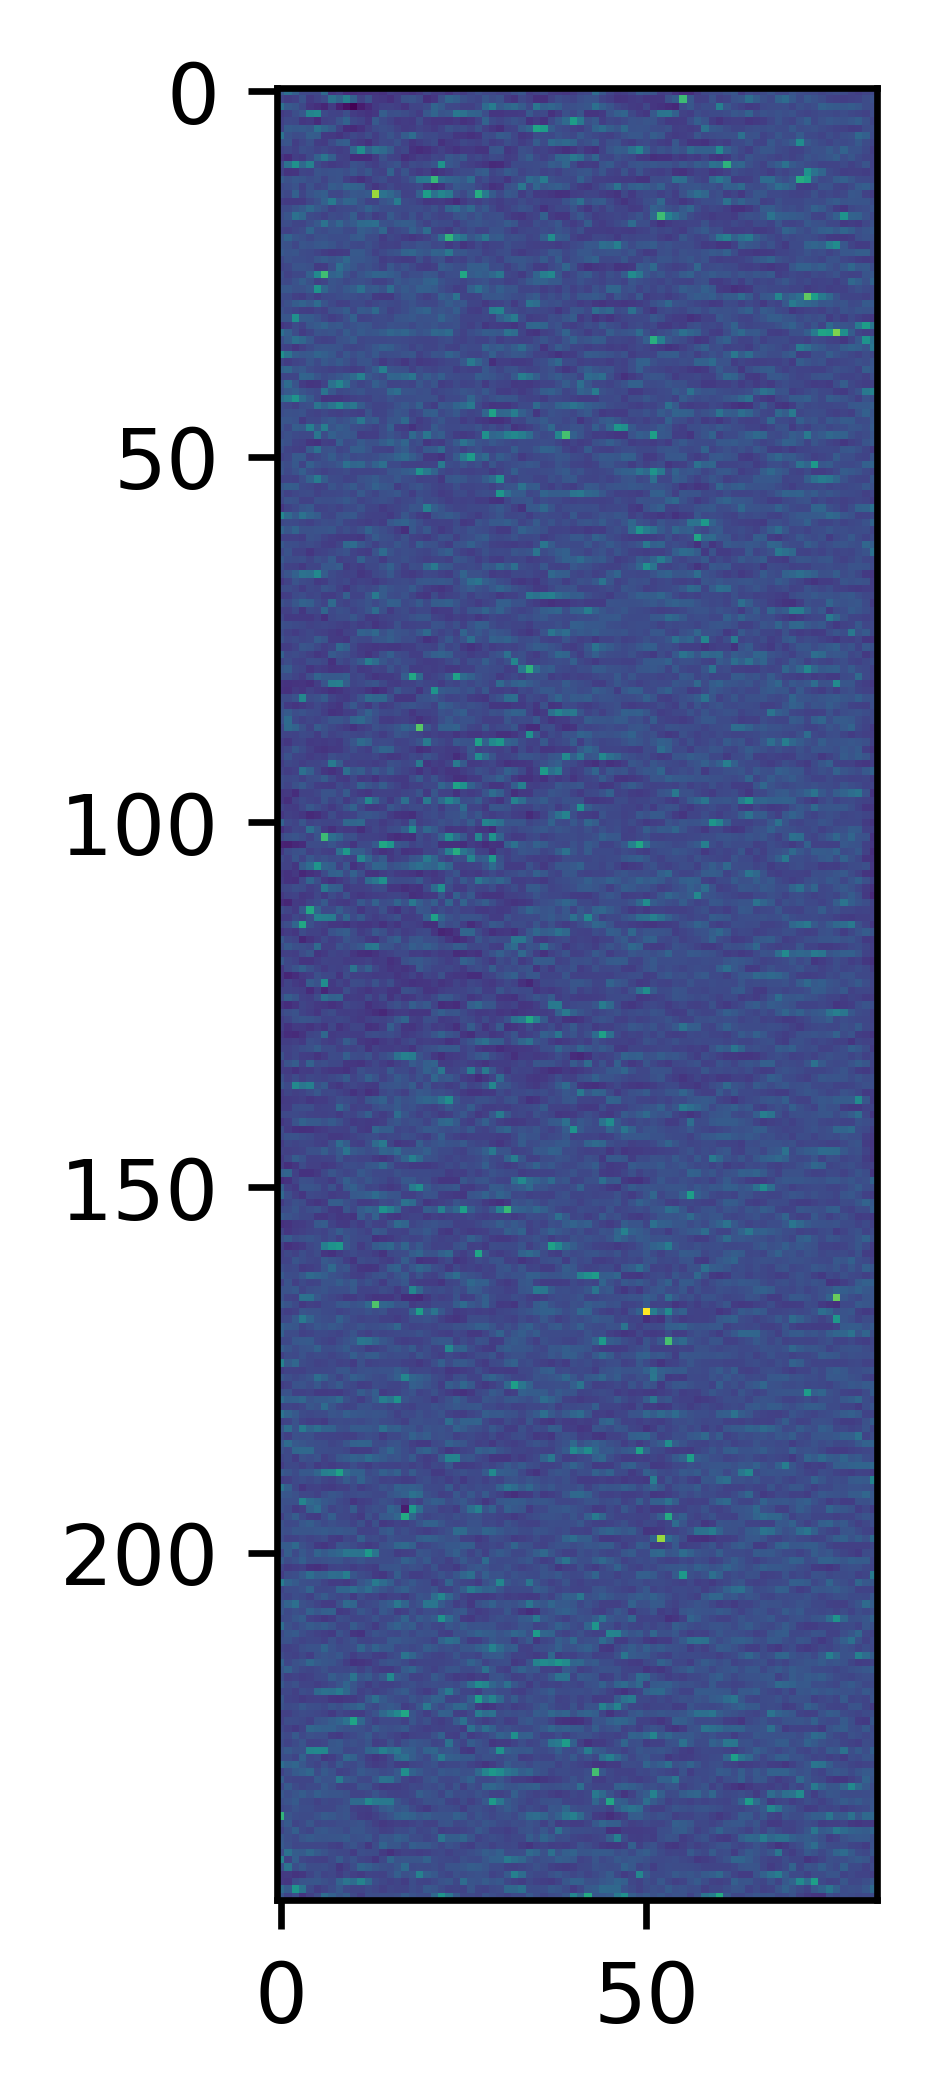
\includegraphics{Graphics/mm-multi-row.png}}
	\subfigure[Por columnas]{\includegraphics{Graphics/mm-multi-col.png}}
	\caption{Resultado de evaluar $\mathbb{S}$ sobre cada una de las \textit{second-rated} de la DST-II usando el tercer enfoque.} \label{fig:example-mm-approach3}
\end{figure}


\begin{figure}
	\centering
	\includegraphics{Graphics/mm-detection-s-on-mm.png}
	\caption{Mamografía con las posiciones predichas por el algoritmo basado en $\mathbb{S}$. Dentro del círculo de color rojo se encuentran dos píxeles que indican estas posiciones.} \label{fig:mm-approach2-mm-s}
\end{figure}

El tercer enfoque no logra buenos resultados, tal y como se muestra en la Figura \ref{fig:example-mm-approach3}.
No se logra ningún signo de detección y, de hecho, los valores no superan $0.8$. 

Como conclusión general de los experimentos, se puede decir que se logró una replicación exitosa de la DST-II,
y que en el caso unidimensional funciona adecuadamente como clasificador para la presencia de un patrón 
dentro de una señal. Sin embargo, una desventaja es el tamaño del patrón. Mientras mayor cantidad
de muestras contenga más díficil es resolver el sistema de ecuaciones no lineales y si el error de la
solución es alto no se logra detección. 
En el caso 2D, ninguno de los enfoques usados para extender este algoritmo al caso
bidimensional fue fructífero. Aunque el segundo enfoque logró hacer detecciones, solo es capaz
de identificar la posición del patrón a través de un único píxel y no sobre una región o
contorno. Esto complica la capacidad de visualizar
dicha detección. Por último, otro aspecto importante es la sensibilidad ante el ruido del algoritmo. 
Aunque la DST-II logre detectar el patrón, modificaciones del mismo son díficiles de detectar.
En el caso de las masas, sus diversos tamaños y formas, no permiten que el algoritmo sea capaz de detectarlas
a partir de un único patrón.

